\documentclass[twoside]{book}

% Packages required by doxygen
\usepackage{calc}
\usepackage{doxygen}
\usepackage{graphicx}
\usepackage[utf8]{inputenc}
\usepackage{makeidx}
\usepackage{multicol}
\usepackage{multirow}
\usepackage{textcomp}
\usepackage[table]{xcolor}

% Font selection
\usepackage[T1]{fontenc}
\usepackage{mathptmx}
\usepackage[scaled=.90]{helvet}
\usepackage{courier}
\usepackage{amssymb}
\usepackage{sectsty}
\renewcommand{\familydefault}{\sfdefault}
\allsectionsfont{%
  \fontseries{bc}\selectfont%
  \color{darkgray}%
}
\renewcommand{\DoxyLabelFont}{%
  \fontseries{bc}\selectfont%
  \color{darkgray}%
}

% Page & text layout
\usepackage{geometry}
\geometry{%
  a4paper,%
  top=2.5cm,%
  bottom=2.5cm,%
  left=2.5cm,%
  right=2.5cm%
}
\tolerance=750
\hfuzz=15pt
\hbadness=750
\setlength{\emergencystretch}{15pt}
\setlength{\parindent}{0cm}
\setlength{\parskip}{0.2cm}
\makeatletter
\renewcommand{\paragraph}{%
  \@startsection{paragraph}{4}{0ex}{-1.0ex}{1.0ex}{%
    \normalfont\normalsize\bfseries\SS@parafont%
  }%
}
\renewcommand{\subparagraph}{%
  \@startsection{subparagraph}{5}{0ex}{-1.0ex}{1.0ex}{%
    \normalfont\normalsize\bfseries\SS@subparafont%
  }%
}
\makeatother

% Headers & footers
\usepackage{fancyhdr}
\pagestyle{fancyplain}
\fancyhead[LE]{\fancyplain{}{\bfseries\thepage}}
\fancyhead[CE]{\fancyplain{}{}}
\fancyhead[RE]{\fancyplain{}{\bfseries\leftmark}}
\fancyhead[LO]{\fancyplain{}{\bfseries\rightmark}}
\fancyhead[CO]{\fancyplain{}{}}
\fancyhead[RO]{\fancyplain{}{\bfseries\thepage}}
\fancyfoot[LE]{\fancyplain{}{}}
\fancyfoot[CE]{\fancyplain{}{}}
\fancyfoot[RE]{\fancyplain{}{\bfseries\scriptsize Generated on Sun Jul 12 2015 17\-:56\-:02 for Meditech control panel software by Doxygen }}
\fancyfoot[LO]{\fancyplain{}{\bfseries\scriptsize Generated on Sun Jul 12 2015 17\-:56\-:02 for Meditech control panel software by Doxygen }}
\fancyfoot[CO]{\fancyplain{}{}}
\fancyfoot[RO]{\fancyplain{}{}}
\renewcommand{\footrulewidth}{0.4pt}
\renewcommand{\chaptermark}[1]{%
  \markboth{#1}{}%
}
\renewcommand{\sectionmark}[1]{%
  \markright{\thesection\ #1}%
}

% Indices & bibliography
\usepackage{natbib}
\usepackage[titles]{tocloft}
\setcounter{tocdepth}{3}
\setcounter{secnumdepth}{5}
\makeindex

% Hyperlinks (required, but should be loaded last)
\usepackage{ifpdf}
\ifpdf
  \usepackage[pdftex,pagebackref=true]{hyperref}
\else
  \usepackage[ps2pdf,pagebackref=true]{hyperref}
\fi
\hypersetup{%
  colorlinks=true,%
  linkcolor=blue,%
  citecolor=blue,%
  unicode%
}

% Custom commands
\newcommand{\clearemptydoublepage}{%
  \newpage{\pagestyle{empty}\cleardoublepage}%
}


%===== C O N T E N T S =====

\begin{document}

% Titlepage & ToC
\hypersetup{pageanchor=false}
\pagenumbering{roman}
\begin{titlepage}
\vspace*{7cm}
\begin{center}%
{\Large Meditech control panel software \\[1ex]\large 1.\-0beta }\\
\vspace*{1cm}
{\large Generated by Doxygen 1.8.6}\\
\vspace*{0.5cm}
{\small Sun Jul 12 2015 17:56:02}\\
\end{center}
\end{titlepage}
\clearemptydoublepage
\tableofcontents
\clearemptydoublepage
\pagenumbering{arabic}
\hypersetup{pageanchor=true}

%--- Begin generated contents ---
\chapter{Main Page}
\label{index}\hypertarget{index}{}This application will run on the Chip\-Kit P\-I module of the Meditech device. The module is connected to the Raspberry P\-I Mod B2. The software includes two parts\-: one independent series of features, related to the Meditech general health status overriding the user controlled parameters. The board also control che alphanumeric \hyperlink{class_l_c_d}{L\-C\-D} display for status messages, warnings and alarms. \par
The user-\/controlled part instead is managed by the Raspberry P\-I \char`\"{}\-P\-I master\char`\"{} controlling the active probes and other functions. The counterpart of this application is a C++ command set running on the P\-I linux machine communicating with the board through a custom serial protocol. To reduce the weight of the microcontroller application most of the strings shown by the control panel display are sent by the linux machine.

\begin{DoxyNote}{Note}
Most of the control panel functions should follow specific priorities, e.\-g. the lid open status while other functions should be exectued periodically byt the board. The high frequency check methods are managed by timer interrupts while the other functions will run in background via the board Task Manager. The use of these two strategies makes the \hyperlink{_meditech___chip_kit_control_panel_8pde_a0b33edabd7f1c4e4a0bf32c67269be2f}{loop()} method more simple and the entire system is more efficient.
\end{DoxyNote}
\begin{DoxyWarning}{Warning}
This code is distributed under the Apache license These sources has been developed under the mpide application, adapted for the Chip\-Kit P\-I board.\par
This application is part of the Meditech project, created by Enrico Miglino for Balearic Dynamics -\/ Balearic Islands -\/ Spain\par
For the last updated application version and subversion, see the \hyperlink{_version_8h}{version.\-h} include file.
\end{DoxyWarning}
\begin{DoxyAuthor}{Author}
Enrico Miglino \href{mailto:enrico.miglino@gmail.com}{\tt enrico.\-miglino@gmail.\-com} 
\end{DoxyAuthor}
\begin{DoxyCopyright}{Copyright}
Balearic Dynamics -\/ Spain \href{mailto:balearicdynamics@gmail.com}{\tt balearicdynamics@gmail.\-com} 
\end{DoxyCopyright}
\begin{DoxyVersion}{Version}
1.\-0b 
\end{DoxyVersion}
\begin{DoxyDate}{Date}
First version on July 2015 
\end{DoxyDate}

\chapter{How L\-C\-D templates works}
\label{lcd_template}
\hypertarget{lcd_template}{}
To simplify the display of the different conditions a set of predefined templates are defined so it is sufficient to send the I\-Ds and relative strings to create the needed visualisation.

This mechanism will also reduce the code size of the program.\par
 Every template has a symbolic I\-D and is built by a simple structure where every string to be shown has its own row and columns. Then a single recursive method can be used to generate the visualisation The templates are though as static objects leaving the space, where needed, for the variable data; in this case the template defines only the position on the display but does not define the content.\par
 Tas the template is an abstraction of the visualisation the strings are not defined statically\-:\par
{\bfseries  the template is filled at runtime}\par
 Every template is an array of a set of basic {\bfseries fields} defining the parameters where a certain value should be shown. 
\chapter{Temperature conversion formulas}
\label{temp_convert}
\hypertarget{temp_convert}{}
The {\ttfamily \hyperlink{class_temperature}{Temperature}} class manages the analog readings from an {\itshape L\-M35} temperature sensor device to control the cooler fan speed.

\par
The base calculation for the temperature after the sensor reading is managed by the {\ttfamily Calc\-Temp} method of the \hyperlink{class_temperature}{Temperature} class; the 10-\/bit A\-D conversion generates 1024 possible values (between 0 and 1023) so the base Celsius float conversion formula is\-:\par
 \begin{center}{\bfseries \mbox{[}sensor\-Value / 1024\mbox{]} $\ast$ 5) $\ast$ 100 }\end{center} 

From this first conversion calculation are derived all the other units values\-: Fahrenheit, Kelvin and Rankine following the formulas below\-:\par
 \begin{center}{\bfseries  Fahrenheit = (Celsius $\ast$ 9) / 5) + 32\par
 Kelvin = Celsius -\/ A\-B\-S\-O\-L\-U\-T\-E\-\_\-\-Z\-E\-R\-O\-\_\-\-C\-E\-L\-S\-I\-U\-S\par
 Rankine = (Celsius -\/ A\-B\-S\-O\-L\-U\-T\-E\-\_\-\-Z\-E\-R\-O\-\_\-\-C\-E\-L\-S\-I\-U\-S) $\ast$ 9) / 5\par
 }\end{center}  
\chapter{Todo List}
\label{todo}
\hypertarget{todo}{}

\begin{DoxyRefList}
\item[\label{todo__todo000002}%
\hypertarget{todo__todo000002}{}%
Member \hyperlink{_command_processor_8h_ab44ed89a60c5bb25c357ce8c3eee91e1}{C\-M\-D\-\_\-\-G\-O} ]Not yet implemented  
\item[\label{todo__todo000001}%
\hypertarget{todo__todo000001}{}%
Member \hyperlink{_command_processor_8h_a775f86e197716388e422fbb58dca826f}{C\-M\-D\-\_\-\-P\-A\-R\-A\-M\-E\-T\-E\-R} ]Not yet implemented  
\item[\label{todo__todo000003}%
\hypertarget{todo__todo000003}{}%
Member \hyperlink{_command_processor_8h_a0a838d0ab7a3cc09b5b9ea002198f36c}{C\-M\-D\-\_\-\-R\-E\-Q\-U\-E\-S\-T} ]Should be implemented in the R\-P\-I master before 

Not yet implemented 

Not yet implemented  
\item[\label{todo__todo000008}%
\hypertarget{todo__todo000008}{}%
Member \hyperlink{_meditech___chip_kit_control_panel_8pde_a40ac0af2d0c4437faa8aebff8336b19b}{set\-Body\-Temp\-Status} (int start\-Char)]Implement this function  
\item[\label{todo__todo000006}%
\hypertarget{todo__todo000006}{}%
Member \hyperlink{_meditech___chip_kit_control_panel_8pde_affc4e4b28b2554dffef9ef55fc1f23a4}{set\-E\-C\-G\-Status} (int start\-Char)]Implement this function  
\item[\label{todo__todo000009}%
\hypertarget{todo__todo000009}{}%
Member \hyperlink{_meditech___chip_kit_control_panel_8pde_aac2c481fecf0a8b7db0babe49a27d1ea}{set\-Heart\-Beat\-Status} (int start\-Char)]Implement this function  
\item[\label{todo__todo000007}%
\hypertarget{todo__todo000007}{}%
Member \hyperlink{_meditech___chip_kit_control_panel_8pde_a962bcf9caf0e8d607a561a6e45c1d4cf}{set\-Pressure\-Status} (int start\-Char)]Implement this function  
\item[\label{todo__todo000005}%
\hypertarget{todo__todo000005}{}%
Member \hyperlink{_meditech___chip_kit_control_panel_8pde_af1fb1c240965fd8ff8ad7ecf88651a0d}{set\-Stethoscope\-Status} (int start\-Char)]Implement this function 
\end{DoxyRefList}
\chapter{Hierarchical Index}
\section{Class Hierarchy}
This inheritance list is sorted roughly, but not completely, alphabetically\-:\begin{DoxyCompactList}
\item Alpha\-L\-C\-D\begin{DoxyCompactList}
\item \contentsline{section}{L\-C\-D}{\pageref{class_l_c_d}}{}
\end{DoxyCompactList}
\item \contentsline{section}{L\-C\-D\-Template\-Field}{\pageref{struct_l_c_d_template_field}}{}
\item \contentsline{section}{L\-C\-D\-Templates}{\pageref{class_l_c_d_templates}}{}
\item \contentsline{section}{parse\-Command}{\pageref{structparse_command}}{}
\item \contentsline{section}{Temperature}{\pageref{class_temperature}}{}
\end{DoxyCompactList}

\chapter{Class Index}
\section{Class List}
Here are the classes, structs, unions and interfaces with brief descriptions\-:\begin{DoxyCompactList}
\item\contentsline{section}{\hyperlink{class_l_c_d}{L\-C\-D} \\*Manages the Alphanumeric display for program output messages }{\pageref{class_l_c_d}}{}
<<<<<<< HEAD
\item\contentsline{section}{\hyperlink{class_l_c_d_stethoscope}{L\-C\-D\-Stethoscope} }{\pageref{class_l_c_d_stethoscope}}{}
\item\contentsline{section}{\hyperlink{struct_l_c_d_template_field}{L\-C\-D\-Template\-Field} \\*\hyperlink{class_l_c_d}{L\-C\-D} template field type definition }{\pageref{struct_l_c_d_template_field}}{}
=======
\item\contentsline{section}{\hyperlink{struct_l_c_d_template_field}{L\-C\-D\-Template\-Field} \\*\hyperlink{class_l_c_d}{L\-C\-D} template field type definition }{\pageref{struct_l_c_d_template_field}}{}
\item\contentsline{section}{\hyperlink{class_l_c_d_templates}{L\-C\-D\-Templates} }{\pageref{class_l_c_d_templates}}{}
>>>>>>> master
\item\contentsline{section}{\hyperlink{structparse_command}{parse\-Command} }{\pageref{structparse_command}}{}
\item\contentsline{section}{\hyperlink{class_temperature}{Temperature} }{\pageref{class_temperature}}{}
\end{DoxyCompactList}

\chapter{File Index}
\section{File List}
Here is a list of all files with brief descriptions\-:\begin{DoxyCompactList}
\item\contentsline{section}{/\-Volumes/\-John Doe/\-Development Projects/\-Meditech Sci\-Fi/\-Sources\-Repositories/chipkit\-\_\-serial\-\_\-pi/\-Meditech\-\_\-\-Chip\-Kit\-Control\-Panel/\hyperlink{_analog_8h}{Analog.\-h} \\*Analog input constants }{\pageref{_analog_8h}}{}
\item\contentsline{section}{/\-Volumes/\-John Doe/\-Development Projects/\-Meditech Sci\-Fi/\-Sources\-Repositories/chipkit\-\_\-serial\-\_\-pi/\-Meditech\-\_\-\-Chip\-Kit\-Control\-Panel/\hyperlink{_command_processor_8h}{Command\-Processor.\-h} \\*Constants and types used by the remote control to manage the behaviour of the board }{\pageref{_command_processor_8h}}{}
\item\contentsline{section}{/\-Volumes/\-John Doe/\-Development Projects/\-Meditech Sci\-Fi/\-Sources\-Repositories/chipkit\-\_\-serial\-\_\-pi/\-Meditech\-\_\-\-Chip\-Kit\-Control\-Panel/\hyperlink{_debug_strings_8h}{Debug\-Strings.\-h} \\*Definition of the debug strings }{\pageref{_debug_strings_8h}}{}
\item\contentsline{section}{/\-Volumes/\-John Doe/\-Development Projects/\-Meditech Sci\-Fi/\-Sources\-Repositories/chipkit\-\_\-serial\-\_\-pi/\-Meditech\-\_\-\-Chip\-Kit\-Control\-Panel/\hyperlink{_globals_8h}{Globals.\-h} \\*Global constants }{\pageref{_globals_8h}}{}
\item\contentsline{section}{/\-Volumes/\-John Doe/\-Development Projects/\-Meditech Sci\-Fi/\-Sources\-Repositories/chipkit\-\_\-serial\-\_\-pi/\-Meditech\-\_\-\-Chip\-Kit\-Control\-Panel/\hyperlink{_l_c_d_8h}{L\-C\-D.\-h} \\*\hyperlink{class_l_c_d}{L\-C\-D} display Manager include file }{\pageref{_l_c_d_8h}}{}
\item\contentsline{section}{/\-Volumes/\-John Doe/\-Development Projects/\-Meditech Sci\-Fi/\-Sources\-Repositories/chipkit\-\_\-serial\-\_\-pi/\-Meditech\-\_\-\-Chip\-Kit\-Control\-Panel/\hyperlink{_l_c_d_templates_8cpp}{L\-C\-D\-Templates.\-cpp} \\*\hyperlink{class_l_c_d}{L\-C\-D} display template class }{\pageref{_l_c_d_templates_8cpp}}{}
\item\contentsline{section}{/\-Volumes/\-John Doe/\-Development Projects/\-Meditech Sci\-Fi/\-Sources\-Repositories/chipkit\-\_\-serial\-\_\-pi/\-Meditech\-\_\-\-Chip\-Kit\-Control\-Panel/\hyperlink{_l_c_d_templates_8h}{L\-C\-D\-Templates.\-h} \\*\hyperlink{class_l_c_d}{L\-C\-D} display templates }{\pageref{_l_c_d_templates_8h}}{}
\item\contentsline{section}{/\-Volumes/\-John Doe/\-Development Projects/\-Meditech Sci\-Fi/\-Sources\-Repositories/chipkit\-\_\-serial\-\_\-pi/\-Meditech\-\_\-\-Chip\-Kit\-Control\-Panel/\hyperlink{_meditech___chip_kit_control_panel_8pde}{Meditech\-\_\-\-Chip\-Kit\-Control\-Panel.\-pde} \\*Meditech Chip\-Kit control panel main application }{\pageref{_meditech___chip_kit_control_panel_8pde}}{}
\item\contentsline{section}{/\-Volumes/\-John Doe/\-Development Projects/\-Meditech Sci\-Fi/\-Sources\-Repositories/chipkit\-\_\-serial\-\_\-pi/\-Meditech\-\_\-\-Chip\-Kit\-Control\-Panel/\hyperlink{_parser_errors_8h}{Parser\-Errors.\-h} \\*Defines the parser error codes }{\pageref{_parser_errors_8h}}{}
\item\contentsline{section}{/\-Volumes/\-John Doe/\-Development Projects/\-Meditech Sci\-Fi/\-Sources\-Repositories/chipkit\-\_\-serial\-\_\-pi/\-Meditech\-\_\-\-Chip\-Kit\-Control\-Panel/\hyperlink{_strings_globals_8h}{Strings\-Globals.\-h} }{\pageref{_strings_globals_8h}}{}
\item\contentsline{section}{/\-Volumes/\-John Doe/\-Development Projects/\-Meditech Sci\-Fi/\-Sources\-Repositories/chipkit\-\_\-serial\-\_\-pi/\-Meditech\-\_\-\-Chip\-Kit\-Control\-Panel/\hyperlink{_temperature_8cpp}{Temperature.\-cpp} \\*Class to manage the internal temperature of the devices }{\pageref{_temperature_8cpp}}{}
\item\contentsline{section}{/\-Volumes/\-John Doe/\-Development Projects/\-Meditech Sci\-Fi/\-Sources\-Repositories/chipkit\-\_\-serial\-\_\-pi/\-Meditech\-\_\-\-Chip\-Kit\-Control\-Panel/\hyperlink{_temperature_8h}{Temperature.\-h} \\*Constants and class prototypes }{\pageref{_temperature_8h}}{}
\item\contentsline{section}{/\-Volumes/\-John Doe/\-Development Projects/\-Meditech Sci\-Fi/\-Sources\-Repositories/chipkit\-\_\-serial\-\_\-pi/\-Meditech\-\_\-\-Chip\-Kit\-Control\-Panel/\hyperlink{_version_8h}{Version.\-h} \\*Version and Build Number Helper Class }{\pageref{_version_8h}}{}
\end{DoxyCompactList}

\chapter{Class Documentation}
\hypertarget{class_l_c_d}{\section{L\-C\-D Class Reference}
\label{class_l_c_d}\index{L\-C\-D@{L\-C\-D}}
}


Manages the Alphanumeric display for program output messages.  




{\ttfamily \#include \char`\"{}L\-C\-D.\-h\char`\"{}}

Inheritance diagram for L\-C\-D\-:\begin{figure}[H]
\begin{center}
\leavevmode
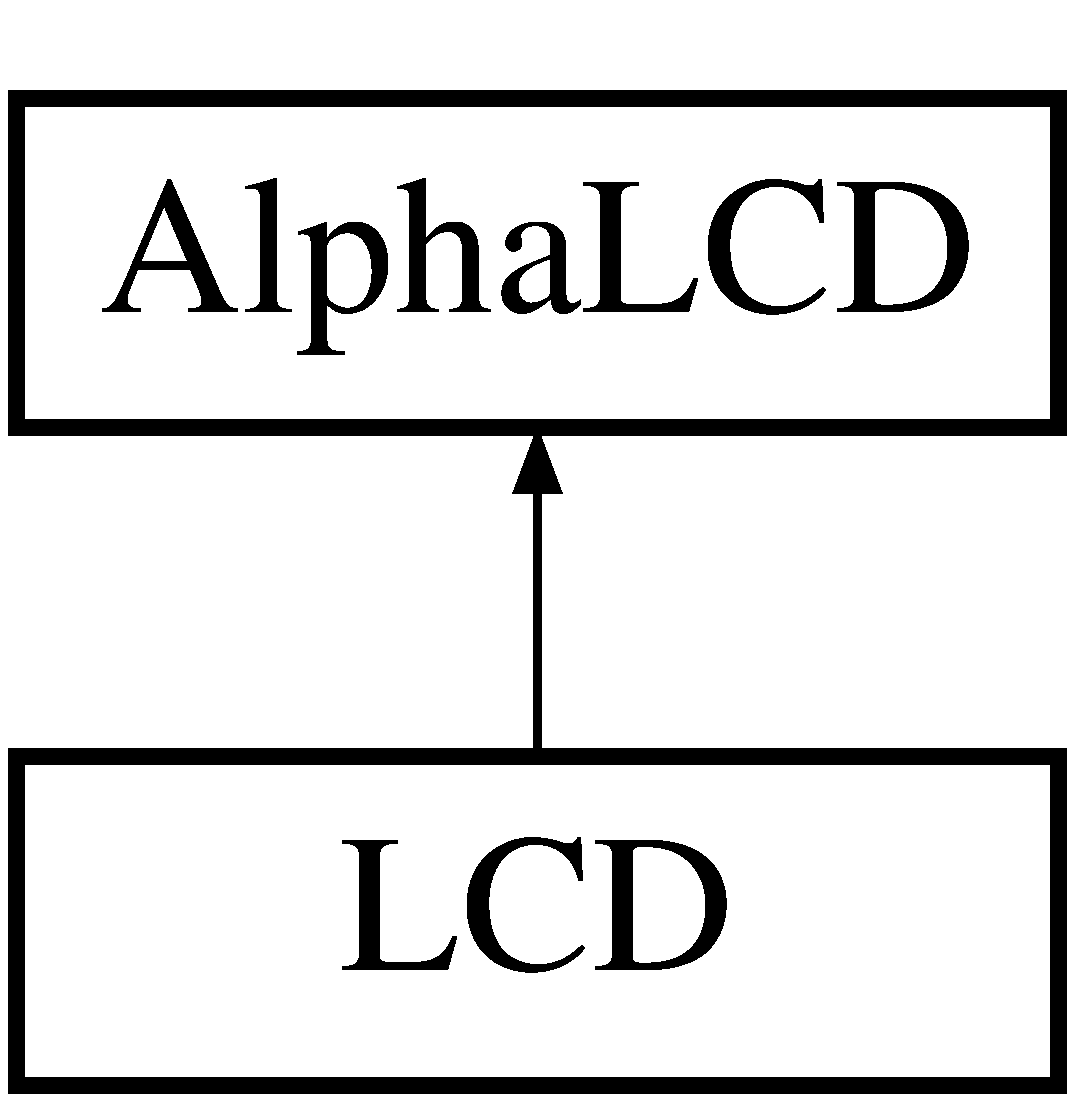
\includegraphics[height=2.000000cm]{class_l_c_d}
\end{center}
\end{figure}
\subsection*{Public Member Functions}
\begin{DoxyCompactItemize}
\item 
\hyperlink{class_l_c_d_a00bb2db1390721abc7b24ac4b8c276c8}{L\-C\-D} ()
\item 
\hyperlink{class_l_c_d_a5ac2667d164486b73b35dce3fd76bd95}{$\sim$\-L\-C\-D} ()
\item 
void \hyperlink{class_l_c_d_a744d30666c9d253089ce10b551854a2f}{enable} (bool s)
\begin{DoxyCompactList}\small\item\em Set the display on or off. \end{DoxyCompactList}\item 
void \hyperlink{class_l_c_d_ad034fa16a3b92276071741d9b31240e5}{blink} (bool set)
\begin{DoxyCompactList}\small\item\em Set blink mode. \end{DoxyCompactList}\item 
void \hyperlink{class_l_c_d_a728c09b7c47d67fc544ed87d06662eb4}{error} (String m)
\begin{DoxyCompactList}\small\item\em shows an error message \end{DoxyCompactList}\item 
void \hyperlink{class_l_c_d_a510e3f387c93e318402163f96d69c2a2}{error} (String m, int x, int y)
\begin{DoxyCompactList}\small\item\em shows an error message at specified coordinates \end{DoxyCompactList}\item 
void \hyperlink{class_l_c_d_a34190efc6a03bb5c0b6cdfff2d7199b9}{message} (String m)
\begin{DoxyCompactList}\small\item\em shows a string message \end{DoxyCompactList}\item 
void \hyperlink{class_l_c_d_a9974c0a77562d699d422992d9bfa1915}{message} (String m, int x, int y)
\begin{DoxyCompactList}\small\item\em shows a string message at specified coordinates \end{DoxyCompactList}\item 
void \hyperlink{class_l_c_d_a0faf36a77c08f7ca19ef7a6df81c3cea}{clean} ()
\begin{DoxyCompactList}\small\item\em clean the \hyperlink{class_l_c_d}{L\-C\-D} screen \end{DoxyCompactList}\item 
void \hyperlink{class_l_c_d_a444c14cc67983cdc179cdf97fda60194}{dec} (int n)
\begin{DoxyCompactList}\small\item\em shows an integer in decimal format \end{DoxyCompactList}\item 
void \hyperlink{class_l_c_d_a3dbdcf6441737a00891f70e472401f77}{hex} (int n)
\begin{DoxyCompactList}\small\item\em shows an integer in hexadeciaml format \end{DoxyCompactList}\item 
void \hyperlink{class_l_c_d_af549238d5b8990cc30115644f4c9138c}{bin} (int n)
\begin{DoxyCompactList}\small\item\em shows an integer in binary format \end{DoxyCompactList}\item 
void \hyperlink{class_l_c_d_ad0b68fbac8b664f506fae6b9af56d366}{oct} (int n)
\begin{DoxyCompactList}\small\item\em shows an integer in octal format \end{DoxyCompactList}\item 
void \hyperlink{class_l_c_d_ac73e78361f5a1004d37b399843d8b5a2}{welcome} ()
\begin{DoxyCompactList}\small\item\em shows the program welcome message \end{DoxyCompactList}\end{DoxyCompactItemize}
\subsection*{Private Member Functions}
\begin{DoxyCompactItemize}
\item 
\hyperlink{class_l_c_d_af0e1f361079353b77e3836eadba85149}{L\-C\-D} (const \hyperlink{class_l_c_d}{L\-C\-D} \&c)
\item 
\hyperlink{class_l_c_d}{L\-C\-D} \& \hyperlink{class_l_c_d_a417d9ed76eb050d25ce6fa6d91c871f1}{operator=} (const \hyperlink{class_l_c_d}{L\-C\-D} \&c)
\end{DoxyCompactItemize}
\subsection*{Private Attributes}
\begin{DoxyCompactItemize}
\item 
Alpha\-L\-C\-D \hyperlink{class_l_c_d_ae4b9e9c4a04d3d976ffb09d112831a5a}{lcd}
\begin{DoxyCompactList}\small\item\em Alpha\-L\-C\-D class inherited instance. \end{DoxyCompactList}\end{DoxyCompactItemize}


\subsection{Detailed Description}
Manages the Alphanumeric display for program output messages. 

This class implements the {\itshape Alpha\-L\-C\-D} class that manages the Alphanumeric \hyperlink{class_l_c_d}{L\-C\-D} display hardware using three digital pins via a shift-\/out register. 

Definition at line 40 of file L\-C\-D.\-h.



\subsection{Constructor \& Destructor Documentation}
\hypertarget{class_l_c_d_a00bb2db1390721abc7b24ac4b8c276c8}{\index{L\-C\-D@{L\-C\-D}!L\-C\-D@{L\-C\-D}}
\index{L\-C\-D@{L\-C\-D}!LCD@{L\-C\-D}}
\subsubsection[{L\-C\-D}]{\setlength{\rightskip}{0pt plus 5cm}L\-C\-D\-::\-L\-C\-D (
\begin{DoxyParamCaption}
{}
\end{DoxyParamCaption}
)}}\label{class_l_c_d_a00bb2db1390721abc7b24ac4b8c276c8}
\hypertarget{class_l_c_d_a5ac2667d164486b73b35dce3fd76bd95}{\index{L\-C\-D@{L\-C\-D}!$\sim$\-L\-C\-D@{$\sim$\-L\-C\-D}}
\index{$\sim$\-L\-C\-D@{$\sim$\-L\-C\-D}!LCD@{L\-C\-D}}
\subsubsection[{$\sim$\-L\-C\-D}]{\setlength{\rightskip}{0pt plus 5cm}L\-C\-D\-::$\sim$\-L\-C\-D (
\begin{DoxyParamCaption}
{}
\end{DoxyParamCaption}
)}}\label{class_l_c_d_a5ac2667d164486b73b35dce3fd76bd95}
\hypertarget{class_l_c_d_af0e1f361079353b77e3836eadba85149}{\index{L\-C\-D@{L\-C\-D}!L\-C\-D@{L\-C\-D}}
\index{L\-C\-D@{L\-C\-D}!LCD@{L\-C\-D}}
\subsubsection[{L\-C\-D}]{\setlength{\rightskip}{0pt plus 5cm}L\-C\-D\-::\-L\-C\-D (
\begin{DoxyParamCaption}
\item[{const {\bf L\-C\-D} \&}]{c}
\end{DoxyParamCaption}
)\hspace{0.3cm}{\ttfamily [private]}}}\label{class_l_c_d_af0e1f361079353b77e3836eadba85149}


\subsection{Member Function Documentation}
\hypertarget{class_l_c_d_af549238d5b8990cc30115644f4c9138c}{\index{L\-C\-D@{L\-C\-D}!bin@{bin}}
\index{bin@{bin}!LCD@{L\-C\-D}}
\subsubsection[{bin}]{\setlength{\rightskip}{0pt plus 5cm}void L\-C\-D\-::bin (
\begin{DoxyParamCaption}
\item[{int}]{n}
\end{DoxyParamCaption}
)}}\label{class_l_c_d_af549238d5b8990cc30115644f4c9138c}


shows an integer in binary format 

\hypertarget{class_l_c_d_ad034fa16a3b92276071741d9b31240e5}{\index{L\-C\-D@{L\-C\-D}!blink@{blink}}
\index{blink@{blink}!LCD@{L\-C\-D}}
\subsubsection[{blink}]{\setlength{\rightskip}{0pt plus 5cm}void L\-C\-D\-::blink (
\begin{DoxyParamCaption}
\item[{bool}]{set}
\end{DoxyParamCaption}
)}}\label{class_l_c_d_ad034fa16a3b92276071741d9b31240e5}


Set blink mode. 

\hypertarget{class_l_c_d_a0faf36a77c08f7ca19ef7a6df81c3cea}{\index{L\-C\-D@{L\-C\-D}!clean@{clean}}
\index{clean@{clean}!LCD@{L\-C\-D}}
\subsubsection[{clean}]{\setlength{\rightskip}{0pt plus 5cm}void L\-C\-D\-::clean (
\begin{DoxyParamCaption}
{}
\end{DoxyParamCaption}
)}}\label{class_l_c_d_a0faf36a77c08f7ca19ef7a6df81c3cea}


clean the \hyperlink{class_l_c_d}{L\-C\-D} screen 

\hypertarget{class_l_c_d_a444c14cc67983cdc179cdf97fda60194}{\index{L\-C\-D@{L\-C\-D}!dec@{dec}}
\index{dec@{dec}!LCD@{L\-C\-D}}
\subsubsection[{dec}]{\setlength{\rightskip}{0pt plus 5cm}void L\-C\-D\-::dec (
\begin{DoxyParamCaption}
\item[{int}]{n}
\end{DoxyParamCaption}
)}}\label{class_l_c_d_a444c14cc67983cdc179cdf97fda60194}


shows an integer in decimal format 

\hypertarget{class_l_c_d_a744d30666c9d253089ce10b551854a2f}{\index{L\-C\-D@{L\-C\-D}!enable@{enable}}
\index{enable@{enable}!LCD@{L\-C\-D}}
\subsubsection[{enable}]{\setlength{\rightskip}{0pt plus 5cm}void L\-C\-D\-::enable (
\begin{DoxyParamCaption}
\item[{bool}]{s}
\end{DoxyParamCaption}
)}}\label{class_l_c_d_a744d30666c9d253089ce10b551854a2f}


Set the display on or off. 

\hypertarget{class_l_c_d_a728c09b7c47d67fc544ed87d06662eb4}{\index{L\-C\-D@{L\-C\-D}!error@{error}}
\index{error@{error}!LCD@{L\-C\-D}}
\subsubsection[{error}]{\setlength{\rightskip}{0pt plus 5cm}void L\-C\-D\-::error (
\begin{DoxyParamCaption}
\item[{String}]{m}
\end{DoxyParamCaption}
)}}\label{class_l_c_d_a728c09b7c47d67fc544ed87d06662eb4}


shows an error message 

\hypertarget{class_l_c_d_a510e3f387c93e318402163f96d69c2a2}{\index{L\-C\-D@{L\-C\-D}!error@{error}}
\index{error@{error}!LCD@{L\-C\-D}}
\subsubsection[{error}]{\setlength{\rightskip}{0pt plus 5cm}void L\-C\-D\-::error (
\begin{DoxyParamCaption}
\item[{String}]{m, }
\item[{int}]{x, }
\item[{int}]{y}
\end{DoxyParamCaption}
)}}\label{class_l_c_d_a510e3f387c93e318402163f96d69c2a2}


shows an error message at specified coordinates 

\hypertarget{class_l_c_d_a3dbdcf6441737a00891f70e472401f77}{\index{L\-C\-D@{L\-C\-D}!hex@{hex}}
\index{hex@{hex}!LCD@{L\-C\-D}}
\subsubsection[{hex}]{\setlength{\rightskip}{0pt plus 5cm}void L\-C\-D\-::hex (
\begin{DoxyParamCaption}
\item[{int}]{n}
\end{DoxyParamCaption}
)}}\label{class_l_c_d_a3dbdcf6441737a00891f70e472401f77}


shows an integer in hexadeciaml format 

\hypertarget{class_l_c_d_a34190efc6a03bb5c0b6cdfff2d7199b9}{\index{L\-C\-D@{L\-C\-D}!message@{message}}
\index{message@{message}!LCD@{L\-C\-D}}
\subsubsection[{message}]{\setlength{\rightskip}{0pt plus 5cm}void L\-C\-D\-::message (
\begin{DoxyParamCaption}
\item[{String}]{m}
\end{DoxyParamCaption}
)}}\label{class_l_c_d_a34190efc6a03bb5c0b6cdfff2d7199b9}


shows a string message 

\hypertarget{class_l_c_d_a9974c0a77562d699d422992d9bfa1915}{\index{L\-C\-D@{L\-C\-D}!message@{message}}
\index{message@{message}!LCD@{L\-C\-D}}
\subsubsection[{message}]{\setlength{\rightskip}{0pt plus 5cm}void L\-C\-D\-::message (
\begin{DoxyParamCaption}
\item[{String}]{m, }
\item[{int}]{x, }
\item[{int}]{y}
\end{DoxyParamCaption}
)}}\label{class_l_c_d_a9974c0a77562d699d422992d9bfa1915}


shows a string message at specified coordinates 

\hypertarget{class_l_c_d_ad0b68fbac8b664f506fae6b9af56d366}{\index{L\-C\-D@{L\-C\-D}!oct@{oct}}
\index{oct@{oct}!LCD@{L\-C\-D}}
\subsubsection[{oct}]{\setlength{\rightskip}{0pt plus 5cm}void L\-C\-D\-::oct (
\begin{DoxyParamCaption}
\item[{int}]{n}
\end{DoxyParamCaption}
)}}\label{class_l_c_d_ad0b68fbac8b664f506fae6b9af56d366}


shows an integer in octal format 

\hypertarget{class_l_c_d_a417d9ed76eb050d25ce6fa6d91c871f1}{\index{L\-C\-D@{L\-C\-D}!operator=@{operator=}}
\index{operator=@{operator=}!LCD@{L\-C\-D}}
\subsubsection[{operator=}]{\setlength{\rightskip}{0pt plus 5cm}{\bf L\-C\-D}\& L\-C\-D\-::operator= (
\begin{DoxyParamCaption}
\item[{const {\bf L\-C\-D} \&}]{c}
\end{DoxyParamCaption}
)\hspace{0.3cm}{\ttfamily [private]}}}\label{class_l_c_d_a417d9ed76eb050d25ce6fa6d91c871f1}
\hypertarget{class_l_c_d_ac73e78361f5a1004d37b399843d8b5a2}{\index{L\-C\-D@{L\-C\-D}!welcome@{welcome}}
\index{welcome@{welcome}!LCD@{L\-C\-D}}
\subsubsection[{welcome}]{\setlength{\rightskip}{0pt plus 5cm}void L\-C\-D\-::welcome (
\begin{DoxyParamCaption}
{}
\end{DoxyParamCaption}
)}}\label{class_l_c_d_ac73e78361f5a1004d37b399843d8b5a2}


shows the program welcome message 



\subsection{Member Data Documentation}
\hypertarget{class_l_c_d_ae4b9e9c4a04d3d976ffb09d112831a5a}{\index{L\-C\-D@{L\-C\-D}!lcd@{lcd}}
\index{lcd@{lcd}!LCD@{L\-C\-D}}
\subsubsection[{lcd}]{\setlength{\rightskip}{0pt plus 5cm}Alpha\-L\-C\-D L\-C\-D\-::lcd\hspace{0.3cm}{\ttfamily [private]}}}\label{class_l_c_d_ae4b9e9c4a04d3d976ffb09d112831a5a}


Alpha\-L\-C\-D class inherited instance. 



Definition at line 45 of file L\-C\-D.\-h.



The documentation for this class was generated from the following file\-:\begin{DoxyCompactItemize}
\item 
/\-Volumes/\-John Doe/\-Development Projects/\-Meditech Sci\-Fi/\-Sources\-Repositories/chipkit\-\_\-serial\-\_\-pi/\-Meditech\-\_\-\-Chip\-Kit\-Control\-Panel/\hyperlink{_l_c_d_8h}{L\-C\-D.\-h}\end{DoxyCompactItemize}

\hypertarget{struct_l_c_d_template_field}{\section{L\-C\-D\-Template\-Field Struct Reference}
\label{struct_l_c_d_template_field}\index{L\-C\-D\-Template\-Field@{L\-C\-D\-Template\-Field}}
}


\hyperlink{class_l_c_d}{L\-C\-D} template field type definition.  




{\ttfamily \#include \char`\"{}L\-C\-D\-Templates.\-h\char`\"{}}

\subsection*{Public Attributes}
\begin{DoxyCompactItemize}
\item 
int \hyperlink{struct_l_c_d_template_field_a842db0224937e139c4ff9f9a6da123e6}{row}
\begin{DoxyCompactList}\small\item\em Field row. \end{DoxyCompactList}\item 
int \hyperlink{struct_l_c_d_template_field_a5dec4293e8f4f297609c83e8612c3f06}{col}
\begin{DoxyCompactList}\small\item\em Field column. \end{DoxyCompactList}\item 
String \hyperlink{struct_l_c_d_template_field_a6eb7ce0547fc28ac3a2538f0fac3f117}{val}
\begin{DoxyCompactList}\small\item\em Field content. \end{DoxyCompactList}\end{DoxyCompactItemize}


\subsection{Detailed Description}
\hyperlink{class_l_c_d}{L\-C\-D} template field type definition. 

Defines a generic \hyperlink{class_l_c_d}{L\-C\-D} display field 

Definition at line 33 of file L\-C\-D\-Templates.\-h.



\subsection{Member Data Documentation}
\hypertarget{struct_l_c_d_template_field_a5dec4293e8f4f297609c83e8612c3f06}{\index{L\-C\-D\-Template\-Field@{L\-C\-D\-Template\-Field}!col@{col}}
\index{col@{col}!LCDTemplateField@{L\-C\-D\-Template\-Field}}
\subsubsection[{col}]{\setlength{\rightskip}{0pt plus 5cm}int L\-C\-D\-Template\-Field\-::col}}\label{struct_l_c_d_template_field_a5dec4293e8f4f297609c83e8612c3f06}


Field column. 



Definition at line 35 of file L\-C\-D\-Templates.\-h.



Referenced by L\-C\-D\-Blood\-Pressure\-::\-L\-C\-D\-Blood\-Pressure(), L\-C\-D\-Default\-::\-L\-C\-D\-Default(), L\-C\-Decg\-::\-L\-C\-Decg(), L\-C\-D\-Heart\-Beat\-::\-L\-C\-D\-Heart\-Beat(), L\-C\-D\-Info\-::\-L\-C\-D\-Info(), L\-C\-D\-Stethoscope\-::\-L\-C\-D\-Stethoscope(), L\-C\-D\-Temperature\-::\-L\-C\-D\-Temperature(), and L\-C\-D\-Test\-::\-L\-C\-D\-Test().

\hypertarget{struct_l_c_d_template_field_a842db0224937e139c4ff9f9a6da123e6}{\index{L\-C\-D\-Template\-Field@{L\-C\-D\-Template\-Field}!row@{row}}
\index{row@{row}!LCDTemplateField@{L\-C\-D\-Template\-Field}}
\subsubsection[{row}]{\setlength{\rightskip}{0pt plus 5cm}int L\-C\-D\-Template\-Field\-::row}}\label{struct_l_c_d_template_field_a842db0224937e139c4ff9f9a6da123e6}


Field row. 



Definition at line 34 of file L\-C\-D\-Templates.\-h.



Referenced by L\-C\-D\-Blood\-Pressure\-::\-L\-C\-D\-Blood\-Pressure(), L\-C\-D\-Default\-::\-L\-C\-D\-Default(), L\-C\-Decg\-::\-L\-C\-Decg(), L\-C\-D\-Heart\-Beat\-::\-L\-C\-D\-Heart\-Beat(), L\-C\-D\-Info\-::\-L\-C\-D\-Info(), L\-C\-D\-Stethoscope\-::\-L\-C\-D\-Stethoscope(), L\-C\-D\-Temperature\-::\-L\-C\-D\-Temperature(), and L\-C\-D\-Test\-::\-L\-C\-D\-Test().

\hypertarget{struct_l_c_d_template_field_a6eb7ce0547fc28ac3a2538f0fac3f117}{\index{L\-C\-D\-Template\-Field@{L\-C\-D\-Template\-Field}!val@{val}}
\index{val@{val}!LCDTemplateField@{L\-C\-D\-Template\-Field}}
\subsubsection[{val}]{\setlength{\rightskip}{0pt plus 5cm}String L\-C\-D\-Template\-Field\-::val}}\label{struct_l_c_d_template_field_a6eb7ce0547fc28ac3a2538f0fac3f117}


Field content. 



Definition at line 36 of file L\-C\-D\-Templates.\-h.



Referenced by L\-C\-D\-Stethoscope\-::create\-Display(), L\-C\-D\-Blood\-Pressure\-::create\-Display(), L\-C\-D\-Heart\-Beat\-::create\-Display(), L\-C\-D\-Temperature\-::create\-Display(), L\-C\-Decg\-::create\-Display(), L\-C\-D\-Test\-::create\-Display(), L\-C\-D\-Info\-::create\-Display(), L\-C\-D\-Default\-::create\-Display(), L\-C\-D\-Stethoscope\-::update\-Display(), L\-C\-D\-Blood\-Pressure\-::update\-Display(), L\-C\-D\-Heart\-Beat\-::update\-Display(), L\-C\-D\-Temperature\-::update\-Display(), and L\-C\-Decg\-::update\-Display().



The documentation for this struct was generated from the following file\-:\begin{DoxyCompactItemize}
\item 
/\-Volumes/\-John Doe/\-Development Projects/\-Meditech Sci\-Fi/\-Sources\-Repositories/chipkit\-\_\-serial\-\_\-pi/\-Meditech\-\_\-\-Chip\-Kit\-Control\-Panel/\hyperlink{_l_c_d_templates_8h}{L\-C\-D\-Templates.\-h}\end{DoxyCompactItemize}

\hypertarget{class_l_c_d_templates}{\section{L\-C\-D\-Templates Class Reference}
\label{class_l_c_d_templates}\index{L\-C\-D\-Templates@{L\-C\-D\-Templates}}
}


{\ttfamily \#include \char`\"{}L\-C\-D\-Templates.\-h\char`\"{}}

\subsection*{Public Member Functions}
\begin{DoxyCompactItemize}
\item 
\hyperlink{class_l_c_d_templates_a4b482ddedce1bcecefa097597b7bb2a4}{L\-C\-D\-Templates} (Alpha\-L\-C\-D my\-L\-C\-D)
\begin{DoxyCompactList}\small\item\em Class constructor. \end{DoxyCompactList}\item 
int \hyperlink{class_l_c_d_templates_a26e2851456f4a2e41b1a57221a29e652}{create\-Display} ()
\begin{DoxyCompactList}\small\item\em Create the full display view parameters. \end{DoxyCompactList}\item 
void \hyperlink{class_l_c_d_templates_a1b01b6974ed1f9433f5926aab699fc84}{update\-Display} (String val, int field\-I\-D)
\begin{DoxyCompactList}\small\item\em Update the variable content field(s) only. \end{DoxyCompactList}\item 
void \hyperlink{class_l_c_d_templates_a9aafd50a26d7bd5178ff7f99ae8a894d}{clean\-Display} ()
\begin{DoxyCompactList}\small\item\em Clean che \hyperlink{class_l_c_d}{L\-C\-D} display area. \end{DoxyCompactList}\end{DoxyCompactItemize}
\subsection*{Public Attributes}
\begin{DoxyCompactItemize}
\item 
int \hyperlink{class_l_c_d_templates_ad5102b181b458439b6714c9b2576f3b2}{id}
\item 
\hyperlink{struct_l_c_d_template_field}{L\-C\-D\-Template\-Field} \hyperlink{class_l_c_d_templates_a804bf1c0e5530bc8f685c52aace5519e}{fields}
\end{DoxyCompactItemize}
\subsection*{Private Attributes}
\begin{DoxyCompactItemize}
\item 
Alpha\-L\-C\-D \hyperlink{class_l_c_d_templates_a92a2475558ce15aa8a311c36705788fd}{m\-Lcd}
\end{DoxyCompactItemize}


\subsection{Detailed Description}


Definition at line 144 of file L\-C\-D\-Templates.\-h.



\subsection{Constructor \& Destructor Documentation}
\hypertarget{class_l_c_d_templates_a4b482ddedce1bcecefa097597b7bb2a4}{\index{L\-C\-D\-Templates@{L\-C\-D\-Templates}!L\-C\-D\-Templates@{L\-C\-D\-Templates}}
\index{L\-C\-D\-Templates@{L\-C\-D\-Templates}!LCDTemplates@{L\-C\-D\-Templates}}
\subsubsection[{L\-C\-D\-Templates}]{\setlength{\rightskip}{0pt plus 5cm}L\-C\-D\-Templates\-::\-L\-C\-D\-Templates (
\begin{DoxyParamCaption}
\item[{Alpha\-L\-C\-D}]{my\-L\-C\-D}
\end{DoxyParamCaption}
)}}\label{class_l_c_d_templates_a4b482ddedce1bcecefa097597b7bb2a4}


Class constructor. 



Definition at line 14 of file L\-C\-D\-Templates.\-cpp.



References m\-Lcd.


\begin{DoxyCode}
14                                          \{
15   \hyperlink{class_l_c_d_templates_a92a2475558ce15aa8a311c36705788fd}{mLcd} = myLCD;
16 \}
\end{DoxyCode}


\subsection{Member Function Documentation}
\hypertarget{class_l_c_d_templates_a9aafd50a26d7bd5178ff7f99ae8a894d}{\index{L\-C\-D\-Templates@{L\-C\-D\-Templates}!clean\-Display@{clean\-Display}}
\index{clean\-Display@{clean\-Display}!LCDTemplates@{L\-C\-D\-Templates}}
\subsubsection[{clean\-Display}]{\setlength{\rightskip}{0pt plus 5cm}void L\-C\-D\-Templates\-::clean\-Display (
\begin{DoxyParamCaption}
{}
\end{DoxyParamCaption}
)}}\label{class_l_c_d_templates_a9aafd50a26d7bd5178ff7f99ae8a894d}


Clean che \hyperlink{class_l_c_d}{L\-C\-D} display area. 



Definition at line 144 of file L\-C\-D\-Templates.\-cpp.



References m\-Lcd.



Referenced by parser().


\begin{DoxyCode}
144                                 \{
145   \hyperlink{class_l_c_d_templates_a92a2475558ce15aa8a311c36705788fd}{mLcd}.clear();
146 \}
\end{DoxyCode}
\hypertarget{class_l_c_d_templates_a26e2851456f4a2e41b1a57221a29e652}{\index{L\-C\-D\-Templates@{L\-C\-D\-Templates}!create\-Display@{create\-Display}}
\index{create\-Display@{create\-Display}!LCDTemplates@{L\-C\-D\-Templates}}
\subsubsection[{create\-Display}]{\setlength{\rightskip}{0pt plus 5cm}int L\-C\-D\-Templates\-::create\-Display (
\begin{DoxyParamCaption}
{}
\end{DoxyParamCaption}
)}}\label{class_l_c_d_templates_a26e2851456f4a2e41b1a57221a29e652}


Create the full display view parameters. 

This method should be called only when the template I\-D has already been set.

\begin{DoxyReturn}{Returns}
The number of fields of the selected template 
\end{DoxyReturn}


Definition at line 26 of file L\-C\-D\-Templates.\-cpp.



References B\-L\-O\-O\-D\-\_\-\-M\-A\-X, B\-L\-O\-O\-D\-\_\-\-M\-A\-X\-V\-A\-L, B\-L\-O\-O\-D\-\_\-\-M\-I\-N, B\-L\-O\-O\-D\-\_\-\-M\-I\-N\-V\-A\-L, B\-L\-O\-O\-D\-\_\-\-T\-I\-T\-L\-E, B\-L\-O\-O\-D\-\_\-\-W\-A\-I\-T, B\-L\-O\-O\-D\-P\-R\-E\-S\-S\-\_\-\-F\-I\-E\-L\-D\-S, L\-C\-D\-Template\-Field\-::col, D\-E\-F\-A\-U\-L\-T\-\_\-\-F\-I\-E\-L\-D\-S, D\-E\-F\-A\-U\-L\-T\-\_\-\-S\-T\-A\-T\-U\-S, D\-E\-F\-A\-U\-L\-T\-\_\-\-T\-I\-T\-L\-E, D\-E\-F\-A\-U\-L\-T\-\_\-\-V\-E\-R\-S\-I\-O\-N, E\-C\-G\-\_\-\-F\-I\-E\-L\-D\-S, E\-C\-G\-\_\-\-S\-T\-A\-T\-U\-S, E\-C\-G\-\_\-\-S\-T\-A\-T\-U\-S\-F\-L\-A\-G, E\-C\-G\-\_\-\-T\-I\-T\-L\-E, fields, H\-E\-A\-R\-T\-B\-E\-A\-T\-\_\-\-A\-V\-E\-R\-A\-G\-E, H\-E\-A\-R\-T\-B\-E\-A\-T\-\_\-\-A\-V\-E\-R\-A\-G\-E\-V\-A\-L, H\-E\-A\-R\-T\-B\-E\-A\-T\-\_\-\-F\-I\-E\-L\-D\-S, H\-E\-A\-R\-T\-B\-E\-A\-T\-\_\-\-S\-P\-O\-T, H\-E\-A\-R\-T\-B\-E\-A\-T\-\_\-\-S\-P\-O\-T\-V\-A\-L, H\-E\-A\-R\-T\-B\-E\-A\-T\-\_\-\-T\-I\-T\-L\-E, I\-N\-F\-O\-\_\-\-D\-A\-T\-E, I\-N\-F\-O\-\_\-\-F\-I\-E\-L\-D\-S, I\-N\-F\-O\-\_\-\-G\-P\-S, I\-N\-F\-O\-\_\-\-R\-P\-M, I\-N\-F\-O\-\_\-\-T\-I\-M\-E, I\-N\-F\-O\-\_\-\-T\-I\-T\-L\-E, L\-C\-D\-Template\-Field\-::row, S\-T\-E\-T\-\_\-\-G\-A\-I\-N, S\-T\-E\-T\-\_\-\-G\-A\-I\-N\-V\-A\-L, S\-T\-E\-T\-\_\-\-T\-I\-T\-L\-E, S\-T\-E\-T\-H\-O\-S\-C\-O\-P\-E\-\_\-\-F\-I\-E\-L\-D\-S, T\-E\-M\-P\-E\-R\-A\-T\-U\-R\-E\-\_\-\-A\-V\-E\-R\-A\-G\-E, T\-E\-M\-P\-E\-R\-A\-T\-U\-R\-E\-\_\-\-A\-V\-E\-R\-A\-G\-E\-V\-A\-L, T\-E\-M\-P\-E\-R\-A\-T\-U\-R\-E\-\_\-\-F\-I\-E\-L\-D\-S, T\-E\-M\-P\-E\-R\-A\-T\-U\-R\-E\-\_\-\-S\-P\-O\-T, T\-E\-M\-P\-E\-R\-A\-T\-U\-R\-E\-\_\-\-S\-P\-O\-T\-V\-A\-L, T\-E\-M\-P\-E\-R\-A\-T\-U\-R\-E\-\_\-\-T\-I\-T\-L\-E, T\-E\-S\-T\-\_\-\-F\-I\-E\-L\-D\-S, T\-E\-S\-T\-\_\-\-S\-T\-A\-T\-U\-S, T\-E\-S\-T\-\_\-\-T\-I\-T\-L\-E, T\-I\-D\-\_\-\-B\-L\-O\-O\-D\-P\-R\-E\-S\-S, T\-I\-D\-\_\-\-D\-E\-F\-A\-U\-L\-T, T\-I\-D\-\_\-\-E\-C\-G, T\-I\-D\-\_\-\-H\-E\-A\-R\-T\-B\-E\-A\-T, T\-I\-D\-\_\-\-I\-N\-F\-O, T\-I\-D\-\_\-\-S\-T\-E\-T\-H\-O\-S\-C\-O\-P\-E, T\-I\-D\-\_\-\-T\-E\-M\-P\-E\-R\-A\-T\-U\-R\-E, and T\-I\-D\-\_\-\-T\-E\-S\-T.



Referenced by parser().


\begin{DoxyCode}
26                                 \{
27   \textcolor{keywordtype}{int} numFields;
28 
29   \textcolor{keywordflow}{switch}(\textcolor{keywordtype}{id}) \{
30     \textcolor{keywordflow}{case} \hyperlink{_l_c_d_templates_8h_ac3ee9f1dc127335a24c11e2dc3a4c024}{TID\_STETHOSCOPE}:
31       \hyperlink{class_l_c_d_templates_a804bf1c0e5530bc8f685c52aace5519e}{fields}.\hyperlink{struct_l_c_d_template_field_a8c1f20c4249d9b0e338609e89499216e}{row}[\hyperlink{_l_c_d_templates_8h_ad52ae2dd0134d3077ab114f680d349e0}{STET\_TITLE}] = 0;
32       \hyperlink{class_l_c_d_templates_a804bf1c0e5530bc8f685c52aace5519e}{fields}.\hyperlink{struct_l_c_d_template_field_acf04ebae1e6cd326e3b4237cb73bb23d}{col}[\hyperlink{_l_c_d_templates_8h_ad52ae2dd0134d3077ab114f680d349e0}{STET\_TITLE}] = 0;
33       \hyperlink{class_l_c_d_templates_a804bf1c0e5530bc8f685c52aace5519e}{fields}.\hyperlink{struct_l_c_d_template_field_a8c1f20c4249d9b0e338609e89499216e}{row}[\hyperlink{_l_c_d_templates_8h_ac0f6206db0de9e1c215be9808bf4b1e1}{STET\_GAIN}] = 1;
34       \hyperlink{class_l_c_d_templates_a804bf1c0e5530bc8f685c52aace5519e}{fields}.\hyperlink{struct_l_c_d_template_field_acf04ebae1e6cd326e3b4237cb73bb23d}{col}[\hyperlink{_l_c_d_templates_8h_ac0f6206db0de9e1c215be9808bf4b1e1}{STET\_GAIN}] = 0;
35       \hyperlink{class_l_c_d_templates_a804bf1c0e5530bc8f685c52aace5519e}{fields}.\hyperlink{struct_l_c_d_template_field_a8c1f20c4249d9b0e338609e89499216e}{row}[\hyperlink{_l_c_d_templates_8h_a99df264a27c8c425105db42a1dbc5fbb}{STET\_GAINVAL}] = 1;
36       \hyperlink{class_l_c_d_templates_a804bf1c0e5530bc8f685c52aace5519e}{fields}.\hyperlink{struct_l_c_d_template_field_acf04ebae1e6cd326e3b4237cb73bb23d}{col}[\hyperlink{_l_c_d_templates_8h_a99df264a27c8c425105db42a1dbc5fbb}{STET\_GAINVAL}] = 12;
37       numFields = \hyperlink{_l_c_d_templates_8h_ab9c573f6265daafe7befb06655294666}{STETHOSCOPE\_FIELDS};
38     \textcolor{keywordflow}{break};
39     \textcolor{keywordflow}{case} \hyperlink{_l_c_d_templates_8h_aaf2c3d4506041e2dc83aa27f28ea6d81}{TID\_BLOODPRESS}:
40       \hyperlink{class_l_c_d_templates_a804bf1c0e5530bc8f685c52aace5519e}{fields}.\hyperlink{struct_l_c_d_template_field_a8c1f20c4249d9b0e338609e89499216e}{row}[\hyperlink{_l_c_d_templates_8h_a300e1cb7e2671b15d4cb72cbc18a9ce7}{BLOOD\_TITLE}] = 0;
41       \hyperlink{class_l_c_d_templates_a804bf1c0e5530bc8f685c52aace5519e}{fields}.\hyperlink{struct_l_c_d_template_field_acf04ebae1e6cd326e3b4237cb73bb23d}{col}[\hyperlink{_l_c_d_templates_8h_a300e1cb7e2671b15d4cb72cbc18a9ce7}{BLOOD\_TITLE}] = 0;
42       \hyperlink{class_l_c_d_templates_a804bf1c0e5530bc8f685c52aace5519e}{fields}.\hyperlink{struct_l_c_d_template_field_a8c1f20c4249d9b0e338609e89499216e}{row}[\hyperlink{_l_c_d_templates_8h_a726eab7d3d8bc5b13a32e1fd8c8d11aa}{BLOOD\_WAIT}] = 1;
43       \hyperlink{class_l_c_d_templates_a804bf1c0e5530bc8f685c52aace5519e}{fields}.\hyperlink{struct_l_c_d_template_field_acf04ebae1e6cd326e3b4237cb73bb23d}{col}[\hyperlink{_l_c_d_templates_8h_a726eab7d3d8bc5b13a32e1fd8c8d11aa}{BLOOD\_WAIT}] = 16;
44       \hyperlink{class_l_c_d_templates_a804bf1c0e5530bc8f685c52aace5519e}{fields}.\hyperlink{struct_l_c_d_template_field_a8c1f20c4249d9b0e338609e89499216e}{row}[\hyperlink{_l_c_d_templates_8h_affc959f533dfb8908431895dda6d1a5e}{BLOOD\_MIN}] = 1;
45       \hyperlink{class_l_c_d_templates_a804bf1c0e5530bc8f685c52aace5519e}{fields}.\hyperlink{struct_l_c_d_template_field_acf04ebae1e6cd326e3b4237cb73bb23d}{col}[\hyperlink{_l_c_d_templates_8h_affc959f533dfb8908431895dda6d1a5e}{BLOOD\_MIN}] = 0;
46       \hyperlink{class_l_c_d_templates_a804bf1c0e5530bc8f685c52aace5519e}{fields}.\hyperlink{struct_l_c_d_template_field_a8c1f20c4249d9b0e338609e89499216e}{row}[\hyperlink{_l_c_d_templates_8h_a764f0d73d432fa04797953292f67ad10}{BLOOD\_MINVAL}] = 1;
47       \hyperlink{class_l_c_d_templates_a804bf1c0e5530bc8f685c52aace5519e}{fields}.\hyperlink{struct_l_c_d_template_field_acf04ebae1e6cd326e3b4237cb73bb23d}{col}[\hyperlink{_l_c_d_templates_8h_a764f0d73d432fa04797953292f67ad10}{BLOOD\_MINVAL}] = 3;
48       \hyperlink{class_l_c_d_templates_a804bf1c0e5530bc8f685c52aace5519e}{fields}.\hyperlink{struct_l_c_d_template_field_a8c1f20c4249d9b0e338609e89499216e}{row}[\hyperlink{_l_c_d_templates_8h_a96b68d70226d7153d39632e4c1a3e83d}{BLOOD\_MAX}] = 1;
49       \hyperlink{class_l_c_d_templates_a804bf1c0e5530bc8f685c52aace5519e}{fields}.\hyperlink{struct_l_c_d_template_field_acf04ebae1e6cd326e3b4237cb73bb23d}{col}[\hyperlink{_l_c_d_templates_8h_a96b68d70226d7153d39632e4c1a3e83d}{BLOOD\_MAX}] = 7;
50       \hyperlink{class_l_c_d_templates_a804bf1c0e5530bc8f685c52aace5519e}{fields}.\hyperlink{struct_l_c_d_template_field_a8c1f20c4249d9b0e338609e89499216e}{row}[\hyperlink{_l_c_d_templates_8h_a7ca44aa5642aff8924996f821049c765}{BLOOD\_MAXVAL}] = 1;
51       \hyperlink{class_l_c_d_templates_a804bf1c0e5530bc8f685c52aace5519e}{fields}.\hyperlink{struct_l_c_d_template_field_acf04ebae1e6cd326e3b4237cb73bb23d}{col}[\hyperlink{_l_c_d_templates_8h_a7ca44aa5642aff8924996f821049c765}{BLOOD\_MAXVAL}] = 9;
52       numFields = \hyperlink{_l_c_d_templates_8h_a31c8ffe16ffc1e2f21020d9f7d972c5d}{BLOODPRESS\_FIELDS};
53     \textcolor{keywordflow}{break};
54     \textcolor{keywordflow}{case} \hyperlink{_l_c_d_templates_8h_a3123215c6e06adef7844e2618c2f44ac}{TID\_HEARTBEAT}:
55       \hyperlink{class_l_c_d_templates_a804bf1c0e5530bc8f685c52aace5519e}{fields}.\hyperlink{struct_l_c_d_template_field_a8c1f20c4249d9b0e338609e89499216e}{row}[\hyperlink{_l_c_d_templates_8h_ad1b8934915b82e46f3f38dcb75b023b8}{HEARTBEAT\_TITLE}] = 0;
56       \hyperlink{class_l_c_d_templates_a804bf1c0e5530bc8f685c52aace5519e}{fields}.\hyperlink{struct_l_c_d_template_field_acf04ebae1e6cd326e3b4237cb73bb23d}{col}[\hyperlink{_l_c_d_templates_8h_ad1b8934915b82e46f3f38dcb75b023b8}{HEARTBEAT\_TITLE}] = 0;
57       \hyperlink{class_l_c_d_templates_a804bf1c0e5530bc8f685c52aace5519e}{fields}.\hyperlink{struct_l_c_d_template_field_a8c1f20c4249d9b0e338609e89499216e}{row}[\hyperlink{_l_c_d_templates_8h_afb5345395c0c48a45a39dd53c84fe1ff}{HEARTBEAT\_SPOT}] = 1;
58       \hyperlink{class_l_c_d_templates_a804bf1c0e5530bc8f685c52aace5519e}{fields}.\hyperlink{struct_l_c_d_template_field_acf04ebae1e6cd326e3b4237cb73bb23d}{col}[\hyperlink{_l_c_d_templates_8h_afb5345395c0c48a45a39dd53c84fe1ff}{HEARTBEAT\_SPOT}] = 0;
59       \hyperlink{class_l_c_d_templates_a804bf1c0e5530bc8f685c52aace5519e}{fields}.\hyperlink{struct_l_c_d_template_field_a8c1f20c4249d9b0e338609e89499216e}{row}[\hyperlink{_l_c_d_templates_8h_a06f4bcc357503298985dc4d8467209a7}{HEARTBEAT\_SPOTVAL}] = 1;
60       \hyperlink{class_l_c_d_templates_a804bf1c0e5530bc8f685c52aace5519e}{fields}.\hyperlink{struct_l_c_d_template_field_acf04ebae1e6cd326e3b4237cb73bb23d}{col}[\hyperlink{_l_c_d_templates_8h_a06f4bcc357503298985dc4d8467209a7}{HEARTBEAT\_SPOTVAL}] = 5;
61       \hyperlink{class_l_c_d_templates_a804bf1c0e5530bc8f685c52aace5519e}{fields}.\hyperlink{struct_l_c_d_template_field_a8c1f20c4249d9b0e338609e89499216e}{row}[\hyperlink{_l_c_d_templates_8h_a810d120fa76c50be46fca1ae99f04aea}{HEARTBEAT\_AVERAGE}] = 1;
62       \hyperlink{class_l_c_d_templates_a804bf1c0e5530bc8f685c52aace5519e}{fields}.\hyperlink{struct_l_c_d_template_field_acf04ebae1e6cd326e3b4237cb73bb23d}{col}[\hyperlink{_l_c_d_templates_8h_a810d120fa76c50be46fca1ae99f04aea}{HEARTBEAT\_AVERAGE}] = 10;
63       \hyperlink{class_l_c_d_templates_a804bf1c0e5530bc8f685c52aace5519e}{fields}.\hyperlink{struct_l_c_d_template_field_a8c1f20c4249d9b0e338609e89499216e}{row}[\hyperlink{_l_c_d_templates_8h_ae384753824d247ec0db88139622c6c64}{HEARTBEAT\_AVERAGEVAL}] = 1;
64       \hyperlink{class_l_c_d_templates_a804bf1c0e5530bc8f685c52aace5519e}{fields}.\hyperlink{struct_l_c_d_template_field_acf04ebae1e6cd326e3b4237cb73bb23d}{col}[\hyperlink{_l_c_d_templates_8h_ae384753824d247ec0db88139622c6c64}{HEARTBEAT\_AVERAGEVAL}] = 15;
65       numFields = \hyperlink{_l_c_d_templates_8h_ac4c63868ab082dc41339237e9bbbca4b}{HEARTBEAT\_FIELDS};
66     \textcolor{keywordflow}{break};
67     \textcolor{keywordflow}{case} \hyperlink{_l_c_d_templates_8h_a4be14e342b55951537f8c2c83ff5ea69}{TID\_TEMPERATURE}:
68       \hyperlink{class_l_c_d_templates_a804bf1c0e5530bc8f685c52aace5519e}{fields}.\hyperlink{struct_l_c_d_template_field_a8c1f20c4249d9b0e338609e89499216e}{row}[\hyperlink{_l_c_d_templates_8h_a5360accba0a796adb2126f6f1a05fede}{TEMPERATURE\_TITLE}] = 0;
69       \hyperlink{class_l_c_d_templates_a804bf1c0e5530bc8f685c52aace5519e}{fields}.\hyperlink{struct_l_c_d_template_field_acf04ebae1e6cd326e3b4237cb73bb23d}{col}[\hyperlink{_l_c_d_templates_8h_a5360accba0a796adb2126f6f1a05fede}{TEMPERATURE\_TITLE}] = 0;
70       \hyperlink{class_l_c_d_templates_a804bf1c0e5530bc8f685c52aace5519e}{fields}.\hyperlink{struct_l_c_d_template_field_a8c1f20c4249d9b0e338609e89499216e}{row}[\hyperlink{_l_c_d_templates_8h_a73bf59d0934c972d759e06578646a87a}{TEMPERATURE\_SPOT}] = 1;
71       \hyperlink{class_l_c_d_templates_a804bf1c0e5530bc8f685c52aace5519e}{fields}.\hyperlink{struct_l_c_d_template_field_acf04ebae1e6cd326e3b4237cb73bb23d}{col}[\hyperlink{_l_c_d_templates_8h_a73bf59d0934c972d759e06578646a87a}{TEMPERATURE\_SPOT}] = 0;
72       \hyperlink{class_l_c_d_templates_a804bf1c0e5530bc8f685c52aace5519e}{fields}.\hyperlink{struct_l_c_d_template_field_a8c1f20c4249d9b0e338609e89499216e}{row}[\hyperlink{_l_c_d_templates_8h_abc5137afa579105d74df895d10440328}{TEMPERATURE\_SPOTVAL}] = 1;
73       \hyperlink{class_l_c_d_templates_a804bf1c0e5530bc8f685c52aace5519e}{fields}.\hyperlink{struct_l_c_d_template_field_acf04ebae1e6cd326e3b4237cb73bb23d}{col}[\hyperlink{_l_c_d_templates_8h_abc5137afa579105d74df895d10440328}{TEMPERATURE\_SPOTVAL}] = 5;
74       \hyperlink{class_l_c_d_templates_a804bf1c0e5530bc8f685c52aace5519e}{fields}.\hyperlink{struct_l_c_d_template_field_a8c1f20c4249d9b0e338609e89499216e}{row}[\hyperlink{_l_c_d_templates_8h_ada3bd806d83529066a4de37b9b6796a0}{TEMPERATURE\_AVERAGE}] = 1;
75       \hyperlink{class_l_c_d_templates_a804bf1c0e5530bc8f685c52aace5519e}{fields}.\hyperlink{struct_l_c_d_template_field_acf04ebae1e6cd326e3b4237cb73bb23d}{col}[\hyperlink{_l_c_d_templates_8h_ada3bd806d83529066a4de37b9b6796a0}{TEMPERATURE\_AVERAGE}] = 10;
76       \hyperlink{class_l_c_d_templates_a804bf1c0e5530bc8f685c52aace5519e}{fields}.\hyperlink{struct_l_c_d_template_field_a8c1f20c4249d9b0e338609e89499216e}{row}[\hyperlink{_l_c_d_templates_8h_a739b23ba909272f259e87d5c533a5f37}{TEMPERATURE\_AVERAGEVAL}] = 1;
77       \hyperlink{class_l_c_d_templates_a804bf1c0e5530bc8f685c52aace5519e}{fields}.\hyperlink{struct_l_c_d_template_field_acf04ebae1e6cd326e3b4237cb73bb23d}{col}[\hyperlink{_l_c_d_templates_8h_a739b23ba909272f259e87d5c533a5f37}{TEMPERATURE\_AVERAGEVAL}] = 15;
78       numFields = \hyperlink{_l_c_d_templates_8h_a111c40e86d424cf6b200349cf1575fda}{TEMPERATURE\_FIELDS};
79     \textcolor{keywordflow}{break};
80     \textcolor{keywordflow}{case} \hyperlink{_l_c_d_templates_8h_aa23412c6cd3b50876409b150c502a843}{TID\_ECG}:
81       \hyperlink{class_l_c_d_templates_a804bf1c0e5530bc8f685c52aace5519e}{fields}.\hyperlink{struct_l_c_d_template_field_a8c1f20c4249d9b0e338609e89499216e}{row}[\hyperlink{_l_c_d_templates_8h_a958623fd7e1c335720d10521696264ef}{ECG\_TITLE}] = 0;
82       \hyperlink{class_l_c_d_templates_a804bf1c0e5530bc8f685c52aace5519e}{fields}.\hyperlink{struct_l_c_d_template_field_acf04ebae1e6cd326e3b4237cb73bb23d}{col}[\hyperlink{_l_c_d_templates_8h_a958623fd7e1c335720d10521696264ef}{ECG\_TITLE}] = 0;
83       \hyperlink{class_l_c_d_templates_a804bf1c0e5530bc8f685c52aace5519e}{fields}.\hyperlink{struct_l_c_d_template_field_a8c1f20c4249d9b0e338609e89499216e}{row}[\hyperlink{_globals_8h_a81c971d1ee27ca31e310c80ef260b390}{ECG\_STATUS}] = 1;
84       \hyperlink{class_l_c_d_templates_a804bf1c0e5530bc8f685c52aace5519e}{fields}.\hyperlink{struct_l_c_d_template_field_acf04ebae1e6cd326e3b4237cb73bb23d}{col}[\hyperlink{_globals_8h_a81c971d1ee27ca31e310c80ef260b390}{ECG\_STATUS}] = 0;
85       \hyperlink{class_l_c_d_templates_a804bf1c0e5530bc8f685c52aace5519e}{fields}.\hyperlink{struct_l_c_d_template_field_a8c1f20c4249d9b0e338609e89499216e}{row}[\hyperlink{_l_c_d_templates_8h_add1c03806c7a5783ed9a7336f4754ab6}{ECG\_STATUSFLAG}] = 1;
86       \hyperlink{class_l_c_d_templates_a804bf1c0e5530bc8f685c52aace5519e}{fields}.\hyperlink{struct_l_c_d_template_field_acf04ebae1e6cd326e3b4237cb73bb23d}{col}[\hyperlink{_l_c_d_templates_8h_add1c03806c7a5783ed9a7336f4754ab6}{ECG\_STATUSFLAG}] = 7;
87       numFields = \hyperlink{_l_c_d_templates_8h_a58b6df1c594707bc5dc5ac6633fe7471}{ECG\_FIELDS};
88     \textcolor{keywordflow}{break};
89     \textcolor{keywordflow}{case} \hyperlink{_l_c_d_templates_8h_a1fa2d890c1a0373f3259708a83a43268}{TID\_TEST}:
90       \hyperlink{class_l_c_d_templates_a804bf1c0e5530bc8f685c52aace5519e}{fields}.\hyperlink{struct_l_c_d_template_field_a8c1f20c4249d9b0e338609e89499216e}{row}[\hyperlink{_l_c_d_templates_8h_afaca57cb825629f8c2fbfec7d343f2dc}{TEST\_TITLE}] = 0;
91       \hyperlink{class_l_c_d_templates_a804bf1c0e5530bc8f685c52aace5519e}{fields}.\hyperlink{struct_l_c_d_template_field_acf04ebae1e6cd326e3b4237cb73bb23d}{col}[\hyperlink{_l_c_d_templates_8h_afaca57cb825629f8c2fbfec7d343f2dc}{TEST\_TITLE}] = 0;
92       \hyperlink{class_l_c_d_templates_a804bf1c0e5530bc8f685c52aace5519e}{fields}.\hyperlink{struct_l_c_d_template_field_a8c1f20c4249d9b0e338609e89499216e}{row}[\hyperlink{_l_c_d_templates_8h_ac9a2283a85840e7f5781e06b288740e9}{TEST\_STATUS}] = 1;
93       \hyperlink{class_l_c_d_templates_a804bf1c0e5530bc8f685c52aace5519e}{fields}.\hyperlink{struct_l_c_d_template_field_acf04ebae1e6cd326e3b4237cb73bb23d}{col}[\hyperlink{_l_c_d_templates_8h_ac9a2283a85840e7f5781e06b288740e9}{TEST\_STATUS}] = 0;
94       numFields = \hyperlink{_l_c_d_templates_8h_a3f6d6cdb1650f9872fb2520b149c4902}{TEST\_FIELDS};
95     \textcolor{keywordflow}{break};
96     \textcolor{keywordflow}{case} \hyperlink{_l_c_d_templates_8h_aff20d279e92773f5794c520a9a9ab212}{TID\_INFO}:
97       \hyperlink{class_l_c_d_templates_a804bf1c0e5530bc8f685c52aace5519e}{fields}.\hyperlink{struct_l_c_d_template_field_a8c1f20c4249d9b0e338609e89499216e}{row}[\hyperlink{_l_c_d_templates_8h_aad7135adf1b88566462acfb21a93cc16}{INFO\_TITLE}] = 0;
98       \hyperlink{class_l_c_d_templates_a804bf1c0e5530bc8f685c52aace5519e}{fields}.\hyperlink{struct_l_c_d_template_field_acf04ebae1e6cd326e3b4237cb73bb23d}{col}[\hyperlink{_l_c_d_templates_8h_aad7135adf1b88566462acfb21a93cc16}{INFO\_TITLE}] = 0;
99       \hyperlink{class_l_c_d_templates_a804bf1c0e5530bc8f685c52aace5519e}{fields}.\hyperlink{struct_l_c_d_template_field_a8c1f20c4249d9b0e338609e89499216e}{row}[\hyperlink{_l_c_d_templates_8h_a9e8e9c4abac12d9fb2b1f568d869265b}{INFO\_RPM}] = 1;
100       \hyperlink{class_l_c_d_templates_a804bf1c0e5530bc8f685c52aace5519e}{fields}.\hyperlink{struct_l_c_d_template_field_acf04ebae1e6cd326e3b4237cb73bb23d}{col}[\hyperlink{_l_c_d_templates_8h_a9e8e9c4abac12d9fb2b1f568d869265b}{INFO\_RPM}] = 16;
101       \hyperlink{class_l_c_d_templates_a804bf1c0e5530bc8f685c52aace5519e}{fields}.\hyperlink{struct_l_c_d_template_field_a8c1f20c4249d9b0e338609e89499216e}{row}[\hyperlink{_l_c_d_templates_8h_a62869db5e003eef6e768cae012519ef4}{INFO\_DATE}] = 0;
102       \hyperlink{class_l_c_d_templates_a804bf1c0e5530bc8f685c52aace5519e}{fields}.\hyperlink{struct_l_c_d_template_field_acf04ebae1e6cd326e3b4237cb73bb23d}{col}[\hyperlink{_l_c_d_templates_8h_a62869db5e003eef6e768cae012519ef4}{INFO\_DATE}] = 4;
103       \hyperlink{class_l_c_d_templates_a804bf1c0e5530bc8f685c52aace5519e}{fields}.\hyperlink{struct_l_c_d_template_field_a8c1f20c4249d9b0e338609e89499216e}{row}[\hyperlink{_l_c_d_templates_8h_a8066428eb5e9fd60743260eb91ac381e}{INFO\_TIME}] = 0;
104       \hyperlink{class_l_c_d_templates_a804bf1c0e5530bc8f685c52aace5519e}{fields}.\hyperlink{struct_l_c_d_template_field_acf04ebae1e6cd326e3b4237cb73bb23d}{col}[\hyperlink{_l_c_d_templates_8h_a8066428eb5e9fd60743260eb91ac381e}{INFO\_TIME}] = 9;
105       \hyperlink{class_l_c_d_templates_a804bf1c0e5530bc8f685c52aace5519e}{fields}.\hyperlink{struct_l_c_d_template_field_a8c1f20c4249d9b0e338609e89499216e}{row}[\hyperlink{_l_c_d_templates_8h_a8b158158e12c49b229f352cd06945182}{INFO\_GPS}] = 1;
106       \hyperlink{class_l_c_d_templates_a804bf1c0e5530bc8f685c52aace5519e}{fields}.\hyperlink{struct_l_c_d_template_field_acf04ebae1e6cd326e3b4237cb73bb23d}{col}[\hyperlink{_l_c_d_templates_8h_a8b158158e12c49b229f352cd06945182}{INFO\_GPS}] = 0;
107       numFields = \hyperlink{_l_c_d_templates_8h_ab5a9c5b13386ff1f3324afcabd2d4c54}{INFO\_FIELDS};
108     \textcolor{keywordflow}{break};
109     \textcolor{keywordflow}{case} \hyperlink{_l_c_d_templates_8h_ab8c87f34cee2394f3eb4c989577e2e8e}{TID\_DEFAULT}:
110       \hyperlink{class_l_c_d_templates_a804bf1c0e5530bc8f685c52aace5519e}{fields}.\hyperlink{struct_l_c_d_template_field_a8c1f20c4249d9b0e338609e89499216e}{row}[\hyperlink{_l_c_d_templates_8h_a6423827ff16ae0e51561df204f8ef9f0}{DEFAULT\_TITLE}] = 0;
111       \hyperlink{class_l_c_d_templates_a804bf1c0e5530bc8f685c52aace5519e}{fields}.\hyperlink{struct_l_c_d_template_field_acf04ebae1e6cd326e3b4237cb73bb23d}{col}[\hyperlink{_l_c_d_templates_8h_a6423827ff16ae0e51561df204f8ef9f0}{DEFAULT\_TITLE}] = 0;
112       \hyperlink{class_l_c_d_templates_a804bf1c0e5530bc8f685c52aace5519e}{fields}.\hyperlink{struct_l_c_d_template_field_a8c1f20c4249d9b0e338609e89499216e}{row}[\hyperlink{_l_c_d_templates_8h_a13dae059206df8d2d9b9b42e694b3f9c}{DEFAULT\_VERSION}] = 1;
113       \hyperlink{class_l_c_d_templates_a804bf1c0e5530bc8f685c52aace5519e}{fields}.\hyperlink{struct_l_c_d_template_field_acf04ebae1e6cd326e3b4237cb73bb23d}{col}[\hyperlink{_l_c_d_templates_8h_a13dae059206df8d2d9b9b42e694b3f9c}{DEFAULT\_VERSION}] = 0;
114       \hyperlink{class_l_c_d_templates_a804bf1c0e5530bc8f685c52aace5519e}{fields}.\hyperlink{struct_l_c_d_template_field_a8c1f20c4249d9b0e338609e89499216e}{row}[\hyperlink{_l_c_d_templates_8h_a188ce67e515b427589d4c363d1132018}{DEFAULT\_STATUS}] = 1;
115       \hyperlink{class_l_c_d_templates_a804bf1c0e5530bc8f685c52aace5519e}{fields}.\hyperlink{struct_l_c_d_template_field_acf04ebae1e6cd326e3b4237cb73bb23d}{col}[\hyperlink{_l_c_d_templates_8h_a188ce67e515b427589d4c363d1132018}{DEFAULT\_STATUS}] = 10;
116       numFields = \hyperlink{_l_c_d_templates_8h_a5024eda36ea0cb0b3f89340f3bb0e146}{DEFAULT\_FIELDS};
117     \textcolor{keywordflow}{break};
118   \}  
119   
120   \textcolor{keywordflow}{return} numFields;
121 \}
\end{DoxyCode}
\hypertarget{class_l_c_d_templates_a1b01b6974ed1f9433f5926aab699fc84}{\index{L\-C\-D\-Templates@{L\-C\-D\-Templates}!update\-Display@{update\-Display}}
\index{update\-Display@{update\-Display}!LCDTemplates@{L\-C\-D\-Templates}}
\subsubsection[{update\-Display}]{\setlength{\rightskip}{0pt plus 5cm}void L\-C\-D\-Templates\-::update\-Display (
\begin{DoxyParamCaption}
\item[{String}]{val, }
\item[{int}]{field\-I\-D}
\end{DoxyParamCaption}
)}}\label{class_l_c_d_templates_a1b01b6974ed1f9433f5926aab699fc84}


Update the variable content field(s) only. 

This method should be called every time the field content of a variable is updated. It affects only the data content fields. To recreate the entire display the \hyperlink{class_l_c_d_templates_a26e2851456f4a2e41b1a57221a29e652}{create\-Display()} method should be called. When the method is called, the class field value is updated after the value conversion.


\begin{DoxyParams}{Parameters}
{\em val} & The string to update \\
\hline
{\em field} & The field I\-D \\
\hline
\end{DoxyParams}


Definition at line 136 of file L\-C\-D\-Templates.\-cpp.



References L\-C\-D\-Template\-Field\-::col, fields, m\-Lcd, and L\-C\-D\-Template\-Field\-::row.



Referenced by parser().


\begin{DoxyCode}
136                                                         \{
137   \hyperlink{class_l_c_d_templates_a92a2475558ce15aa8a311c36705788fd}{mLcd}.setCursor(\hyperlink{class_l_c_d_templates_a804bf1c0e5530bc8f685c52aace5519e}{fields}.\hyperlink{struct_l_c_d_template_field_acf04ebae1e6cd326e3b4237cb73bb23d}{col}[fieldID], \hyperlink{class_l_c_d_templates_a804bf1c0e5530bc8f685c52aace5519e}{fields}.\hyperlink{struct_l_c_d_template_field_a8c1f20c4249d9b0e338609e89499216e}{row}[fieldID]);
138   \hyperlink{class_l_c_d_templates_a92a2475558ce15aa8a311c36705788fd}{mLcd} << val;
139 \}
\end{DoxyCode}


\subsection{Member Data Documentation}
\hypertarget{class_l_c_d_templates_a804bf1c0e5530bc8f685c52aace5519e}{\index{L\-C\-D\-Templates@{L\-C\-D\-Templates}!fields@{fields}}
\index{fields@{fields}!LCDTemplates@{L\-C\-D\-Templates}}
\subsubsection[{fields}]{\setlength{\rightskip}{0pt plus 5cm}{\bf L\-C\-D\-Template\-Field} L\-C\-D\-Templates\-::fields}}\label{class_l_c_d_templates_a804bf1c0e5530bc8f685c52aace5519e}


Definition at line 151 of file L\-C\-D\-Templates.\-h.



Referenced by create\-Display(), and update\-Display().

\hypertarget{class_l_c_d_templates_ad5102b181b458439b6714c9b2576f3b2}{\index{L\-C\-D\-Templates@{L\-C\-D\-Templates}!id@{id}}
\index{id@{id}!LCDTemplates@{L\-C\-D\-Templates}}
\subsubsection[{id}]{\setlength{\rightskip}{0pt plus 5cm}int L\-C\-D\-Templates\-::id}}\label{class_l_c_d_templates_ad5102b181b458439b6714c9b2576f3b2}


Definition at line 150 of file L\-C\-D\-Templates.\-h.



Referenced by parser().

\hypertarget{class_l_c_d_templates_a92a2475558ce15aa8a311c36705788fd}{\index{L\-C\-D\-Templates@{L\-C\-D\-Templates}!m\-Lcd@{m\-Lcd}}
\index{m\-Lcd@{m\-Lcd}!LCDTemplates@{L\-C\-D\-Templates}}
\subsubsection[{m\-Lcd}]{\setlength{\rightskip}{0pt plus 5cm}Alpha\-L\-C\-D L\-C\-D\-Templates\-::m\-Lcd\hspace{0.3cm}{\ttfamily [private]}}}\label{class_l_c_d_templates_a92a2475558ce15aa8a311c36705788fd}


Definition at line 153 of file L\-C\-D\-Templates.\-h.



Referenced by clean\-Display(), L\-C\-D\-Templates(), and update\-Display().



The documentation for this class was generated from the following files\-:\begin{DoxyCompactItemize}
\item 
/\-Volumes/\-John Doe/\-Development Projects/\-Meditech Sci\-Fi/\-Sources\-Repositories/chipkit\-\_\-serial\-\_\-pi/\-Meditech\-\_\-\-Chip\-Kit\-Control\-Panel/\hyperlink{_l_c_d_templates_8h}{L\-C\-D\-Templates.\-h}\item 
/\-Volumes/\-John Doe/\-Development Projects/\-Meditech Sci\-Fi/\-Sources\-Repositories/chipkit\-\_\-serial\-\_\-pi/\-Meditech\-\_\-\-Chip\-Kit\-Control\-Panel/\hyperlink{_l_c_d_templates_8cpp}{L\-C\-D\-Templates.\-cpp}\end{DoxyCompactItemize}

\hypertarget{structparse_command}{\section{parse\-Command Struct Reference}
\label{structparse_command}\index{parse\-Command@{parse\-Command}}
}


{\ttfamily \#include \char`\"{}Command\-Processor.\-h\char`\"{}}

\subsection*{Public Attributes}
\begin{DoxyCompactItemize}
\item 
char \hyperlink{structparse_command_a10312bf6b72a9315a4fb550458bc3ae9}{subcommand} \mbox{[}1\mbox{]}
\begin{DoxyCompactList}\small\item\em char subcommand\mbox{[}1\mbox{]} Contains the last parsed subcommand \end{DoxyCompactList}\item 
<<<<<<< HEAD
char \hyperlink{structparse_command_ab80399acc713a2d31a48dd2db5c7d0a2}{message} \mbox{[}20\mbox{]}
\begin{DoxyCompactList}\small\item\em Command associated message string, used by S\-\_\-\-S\-U\-B\-S\-T\-R\-I\-N\-G, C\-M\-D\-\_\-\-W\-R\-I\-T\-E, C\-M\-D\-\_\-\-E\-X\-E\-C. \end{DoxyCompactList}\item 
long \hyperlink{structparse_command_ad062df88615d7d66ded447dd4ff87bad}{long\-Value}
\begin{DoxyCompactList}\small\item\em Generic long parameter. \end{DoxyCompactList}\item 
int \hyperlink{structparse_command_a022bdea84dc5c07ff20af8690a1aa2e3}{int\-Value}
\begin{DoxyCompactList}\small\item\em Generic integer parameter. \end{DoxyCompactList}\item 
float \hyperlink{structparse_command_a121ded5fdf791ba216ad84cef651fe74}{float\-Value}
\begin{DoxyCompactList}\small\item\em Generic float parameter. \end{DoxyCompactList}\item 
int \hyperlink{structparse_command_a5f5c48be92f3aae7c4b1b71ca750298b}{separator}
\begin{DoxyCompactList}\small\item\em Separator character. \end{DoxyCompactList}\item 
char \hyperlink{structparse_command_a7cb5165cf18cc63d7eed9fa34be4efd8}{cmd\-Data} \mbox{[}160\mbox{]}
\begin{DoxyCompactList}\small\item\em Unparsed Command String. \end{DoxyCompactList}\end{DoxyCompactItemize}
=======
String \hyperlink{structparse_command_a5d2f84606922f34ad6a8ca5f7d8a59b5}{message}
\begin{DoxyCompactList}\small\item\em Command associated message string, used to return messages to the master and sending requests. The string should not be longer than C\-M\-D\-\_\-\-M\-S\-G\-L\-E\-N. \end{DoxyCompactList}\item 
int \hyperlink{structparse_command_a8359e121af4d2f16e054ead0b7844a30}{command\-Length}
\begin{DoxyCompactList}\small\item\em The number of characters collected by the last lines read buffer from serial. \end{DoxyCompactList}\item 
String \hyperlink{structparse_command_ac5ece0b161e3fae794d08911247c0b1e}{string\-Value}
\begin{DoxyCompactList}\small\item\em Returning parameter from the command parser. \end{DoxyCompactList}\item 
long \hyperlink{structparse_command_a10deac33dc255dd8a8b84532bbeb6c42}{long\-Value} \mbox{[}2\mbox{]}
\begin{DoxyCompactList}\small\item\em Returning parameter from the command parser The array number of position is the longer number of type parameters in a command. \end{DoxyCompactList}\item 
int \hyperlink{structparse_command_a9ad775810b79683631510fd333096c6f}{int\-Value} \mbox{[}2\mbox{]}
\begin{DoxyCompactList}\small\item\em Returning parameter from the command parser The array number of position is the longer number of type parameters in a command. \end{DoxyCompactList}\item 
float \hyperlink{structparse_command_a475f06e9e3728cc583008ad66dc48329}{float\-Value} \mbox{[}2\mbox{]}
\begin{DoxyCompactList}\small\item\em Returning parameter from the command parser The array number of position is the longer number of type parameters in a command. \end{DoxyCompactList}\item 
float \hyperlink{structparse_command_aff75594be6413210138456dc4572be52}{boolean\-Value}
\begin{DoxyCompactList}\small\item\em Returning parameter from the command parser. \end{DoxyCompactList}\end{DoxyCompactItemize}
>>>>>>> master


\subsection{Detailed Description}


<<<<<<< HEAD
Definition at line 53 of file Command\-Processor.\-h.
=======
Definition at line 79 of file Command\-Processor.\-h.
>>>>>>> master



\subsection{Member Data Documentation}
<<<<<<< HEAD
\hypertarget{structparse_command_a7cb5165cf18cc63d7eed9fa34be4efd8}{\index{parse\-Command@{parse\-Command}!cmd\-Data@{cmd\-Data}}
\index{cmd\-Data@{cmd\-Data}!parseCommand@{parse\-Command}}
\subsubsection[{cmd\-Data}]{\setlength{\rightskip}{0pt plus 5cm}char parse\-Command\-::cmd\-Data\mbox{[}160\mbox{]}}}\label{structparse_command_a7cb5165cf18cc63d7eed9fa34be4efd8}


Unparsed Command String. 

cmd\-Data is the string after syntax checking. The string can contain one or more commands. When the command string is sent to the parser this value contains the command sequence. When the this string is empy all the commands has been processed and the system is ready to receive a new command. 

Definition at line 76 of file Command\-Processor.\-h.

\hypertarget{structparse_command_a121ded5fdf791ba216ad84cef651fe74}{\index{parse\-Command@{parse\-Command}!float\-Value@{float\-Value}}
\index{float\-Value@{float\-Value}!parseCommand@{parse\-Command}}
\subsubsection[{float\-Value}]{\setlength{\rightskip}{0pt plus 5cm}float parse\-Command\-::float\-Value}}\label{structparse_command_a121ded5fdf791ba216ad84cef651fe74}


Generic float parameter. 



Definition at line 63 of file Command\-Processor.\-h.

\hypertarget{structparse_command_a022bdea84dc5c07ff20af8690a1aa2e3}{\index{parse\-Command@{parse\-Command}!int\-Value@{int\-Value}}
\index{int\-Value@{int\-Value}!parseCommand@{parse\-Command}}
\subsubsection[{int\-Value}]{\setlength{\rightskip}{0pt plus 5cm}int parse\-Command\-::int\-Value}}\label{structparse_command_a022bdea84dc5c07ff20af8690a1aa2e3}


Generic integer parameter. 



Definition at line 62 of file Command\-Processor.\-h.

\hypertarget{structparse_command_ad062df88615d7d66ded447dd4ff87bad}{\index{parse\-Command@{parse\-Command}!long\-Value@{long\-Value}}
\index{long\-Value@{long\-Value}!parseCommand@{parse\-Command}}
\subsubsection[{long\-Value}]{\setlength{\rightskip}{0pt plus 5cm}long parse\-Command\-::long\-Value}}\label{structparse_command_ad062df88615d7d66ded447dd4ff87bad}


Generic long parameter. 



Definition at line 61 of file Command\-Processor.\-h.

\hypertarget{structparse_command_ab80399acc713a2d31a48dd2db5c7d0a2}{\index{parse\-Command@{parse\-Command}!message@{message}}
\index{message@{message}!parseCommand@{parse\-Command}}
\subsubsection[{message}]{\setlength{\rightskip}{0pt plus 5cm}char parse\-Command\-::message\mbox{[}20\mbox{]}}}\label{structparse_command_ab80399acc713a2d31a48dd2db5c7d0a2}


Command associated message string, used by S\-\_\-\-S\-U\-B\-S\-T\-R\-I\-N\-G, C\-M\-D\-\_\-\-W\-R\-I\-T\-E, C\-M\-D\-\_\-\-E\-X\-E\-C. 



Definition at line 59 of file Command\-Processor.\-h.

\hypertarget{structparse_command_a5f5c48be92f3aae7c4b1b71ca750298b}{\index{parse\-Command@{parse\-Command}!separator@{separator}}
\index{separator@{separator}!parseCommand@{parse\-Command}}
\subsubsection[{separator}]{\setlength{\rightskip}{0pt plus 5cm}int parse\-Command\-::separator}}\label{structparse_command_a5f5c48be92f3aae7c4b1b71ca750298b}


Separator character. 



Definition at line 64 of file Command\-Processor.\-h.
=======
\hypertarget{structparse_command_aff75594be6413210138456dc4572be52}{\index{parse\-Command@{parse\-Command}!boolean\-Value@{boolean\-Value}}
\index{boolean\-Value@{boolean\-Value}!parseCommand@{parse\-Command}}
\subsubsection[{boolean\-Value}]{\setlength{\rightskip}{0pt plus 5cm}float parse\-Command\-::boolean\-Value}}\label{structparse_command_aff75594be6413210138456dc4572be52}


Returning parameter from the command parser. 



Definition at line 107 of file Command\-Processor.\-h.

\hypertarget{structparse_command_a8359e121af4d2f16e054ead0b7844a30}{\index{parse\-Command@{parse\-Command}!command\-Length@{command\-Length}}
\index{command\-Length@{command\-Length}!parseCommand@{parse\-Command}}
\subsubsection[{command\-Length}]{\setlength{\rightskip}{0pt plus 5cm}int parse\-Command\-::command\-Length}}\label{structparse_command_a8359e121af4d2f16e054ead0b7844a30}


The number of characters collected by the last lines read buffer from serial. 



Definition at line 90 of file Command\-Processor.\-h.



Referenced by check\-Serial(), and parser().

\hypertarget{structparse_command_a475f06e9e3728cc583008ad66dc48329}{\index{parse\-Command@{parse\-Command}!float\-Value@{float\-Value}}
\index{float\-Value@{float\-Value}!parseCommand@{parse\-Command}}
\subsubsection[{float\-Value}]{\setlength{\rightskip}{0pt plus 5cm}float parse\-Command\-::float\-Value\mbox{[}2\mbox{]}}}\label{structparse_command_a475f06e9e3728cc583008ad66dc48329}


Returning parameter from the command parser The array number of position is the longer number of type parameters in a command. 



Definition at line 105 of file Command\-Processor.\-h.

\hypertarget{structparse_command_a9ad775810b79683631510fd333096c6f}{\index{parse\-Command@{parse\-Command}!int\-Value@{int\-Value}}
\index{int\-Value@{int\-Value}!parseCommand@{parse\-Command}}
\subsubsection[{int\-Value}]{\setlength{\rightskip}{0pt plus 5cm}int parse\-Command\-::int\-Value\mbox{[}2\mbox{]}}}\label{structparse_command_a9ad775810b79683631510fd333096c6f}


Returning parameter from the command parser The array number of position is the longer number of type parameters in a command. 



Definition at line 101 of file Command\-Processor.\-h.



Referenced by parser().

\hypertarget{structparse_command_a10deac33dc255dd8a8b84532bbeb6c42}{\index{parse\-Command@{parse\-Command}!long\-Value@{long\-Value}}
\index{long\-Value@{long\-Value}!parseCommand@{parse\-Command}}
\subsubsection[{long\-Value}]{\setlength{\rightskip}{0pt plus 5cm}long parse\-Command\-::long\-Value\mbox{[}2\mbox{]}}}\label{structparse_command_a10deac33dc255dd8a8b84532bbeb6c42}


Returning parameter from the command parser The array number of position is the longer number of type parameters in a command. 



Definition at line 97 of file Command\-Processor.\-h.

\hypertarget{structparse_command_a5d2f84606922f34ad6a8ca5f7d8a59b5}{\index{parse\-Command@{parse\-Command}!message@{message}}
\index{message@{message}!parseCommand@{parse\-Command}}
\subsubsection[{message}]{\setlength{\rightskip}{0pt plus 5cm}String parse\-Command\-::message}}\label{structparse_command_a5d2f84606922f34ad6a8ca5f7d8a59b5}


Command associated message string, used to return messages to the master and sending requests. The string should not be longer than C\-M\-D\-\_\-\-M\-S\-G\-L\-E\-N. 



Definition at line 86 of file Command\-Processor.\-h.



Referenced by ack\-Master(), append\-Response(), and parser().

\hypertarget{structparse_command_ac5ece0b161e3fae794d08911247c0b1e}{\index{parse\-Command@{parse\-Command}!string\-Value@{string\-Value}}
\index{string\-Value@{string\-Value}!parseCommand@{parse\-Command}}
\subsubsection[{string\-Value}]{\setlength{\rightskip}{0pt plus 5cm}String parse\-Command\-::string\-Value}}\label{structparse_command_ac5ece0b161e3fae794d08911247c0b1e}


Returning parameter from the command parser. 



Definition at line 93 of file Command\-Processor.\-h.



Referenced by parser().
>>>>>>> master

\hypertarget{structparse_command_a10312bf6b72a9315a4fb550458bc3ae9}{\index{parse\-Command@{parse\-Command}!subcommand@{subcommand}}
\index{subcommand@{subcommand}!parseCommand@{parse\-Command}}
\subsubsection[{subcommand}]{\setlength{\rightskip}{0pt plus 5cm}char parse\-Command\-::subcommand\mbox{[}1\mbox{]}}}\label{structparse_command_a10312bf6b72a9315a4fb550458bc3ae9}


char subcommand\mbox{[}1\mbox{]} Contains the last parsed subcommand 



<<<<<<< HEAD
Definition at line 57 of file Command\-Processor.\-h.
=======
Definition at line 82 of file Command\-Processor.\-h.



Referenced by parser().
>>>>>>> master



The documentation for this struct was generated from the following file\-:\begin{DoxyCompactItemize}
\item 
/\-Volumes/\-John Doe/\-Development Projects/\-Meditech Sci\-Fi/\-Sources\-Repositories/chipkit\-\_\-serial\-\_\-pi/\-Meditech\-\_\-\-Chip\-Kit\-Control\-Panel/\hyperlink{_command_processor_8h}{Command\-Processor.\-h}\end{DoxyCompactItemize}

\hypertarget{class_temperature}{\section{Temperature Class Reference}
\label{class_temperature}\index{Temperature@{Temperature}}
}


{\ttfamily \#include \char`\"{}Temperature.\-h\char`\"{}}

\subsection*{Public Member Functions}
\begin{DoxyCompactItemize}
\item 
\hyperlink{class_temperature_ab8f4f9e793a8e4f35eed33c240bbe278}{Temperature} ()
\begin{DoxyCompactList}\small\item\em \hyperlink{class_temperature}{Temperature} class constructor. \end{DoxyCompactList}\item 
void \hyperlink{class_temperature_a909c328fd6235d0e7c8ea110a1fb201d}{Calc\-Temp} (float sensor)
\begin{DoxyCompactList}\small\item\em Convert the analog value to the respective value. \end{DoxyCompactList}\item 
float \hyperlink{class_temperature_a3cb76ed5fdb2227d59a6759c1e9938d8}{Celsius} () const 
\begin{DoxyCompactList}\small\item\em Return the last temperature read in Celsius deg. \end{DoxyCompactList}\item 
float \hyperlink{class_temperature_ab0833daedc73ca32235680fa4aa6c664}{Fahrenheit} () const 
\begin{DoxyCompactList}\small\item\em Return the last temperature read in Fahrenheit deg. \end{DoxyCompactList}\item 
float \hyperlink{class_temperature_a0abbc7cb4f86d2305f9633dfc74f0228}{Kelvin} () const 
\begin{DoxyCompactList}\small\item\em Return the last temperature read in Kelvin deg. \end{DoxyCompactList}\item 
float \hyperlink{class_temperature_a63f20b0118f0ea69bb3172c65511ab65}{Rankine} () const 
\begin{DoxyCompactList}\small\item\em Return the last temperature read in Rankine deg. \end{DoxyCompactList}\end{DoxyCompactItemize}
\subsection*{Private Attributes}
\begin{DoxyCompactItemize}
\item 
float \hyperlink{class_temperature_a847274ce6df795e801620cd7cd0247ef}{\-\_\-\-Celsius}
\item 
float \hyperlink{class_temperature_a0beb140a271261eb89c3f2fb3bd1f4db}{\-\_\-\-Fahrenheit}
\item 
float \hyperlink{class_temperature_a832a839960e688420e234a9ccfbc363e}{\-\_\-\-Kelvin}
\item 
float \hyperlink{class_temperature_a3934bf7760e98ece1f0d1487051e6c6e}{\-\_\-\-Rankine}
\item 
float \hyperlink{class_temperature_a827e297c3c400d55542b6125626e4de1}{\-\_\-sensor\-Value}
\end{DoxyCompactItemize}


\subsection{Detailed Description}


Definition at line 22 of file Temperature.\-h.



\subsection{Constructor \& Destructor Documentation}
\hypertarget{class_temperature_ab8f4f9e793a8e4f35eed33c240bbe278}{\index{Temperature@{Temperature}!Temperature@{Temperature}}
\index{Temperature@{Temperature}!Temperature@{Temperature}}
\subsubsection[{Temperature}]{\setlength{\rightskip}{0pt plus 5cm}Temperature\-::\-Temperature (
\begin{DoxyParamCaption}
{}
\end{DoxyParamCaption}
)}}\label{class_temperature_ab8f4f9e793a8e4f35eed33c240bbe278}


\hyperlink{class_temperature}{Temperature} class constructor. 

Set the analog pin for data reading 

Definition at line 31 of file Temperature.\-cpp.


\begin{DoxyCode}
31                           \{
32  \} 
\end{DoxyCode}


\subsection{Member Function Documentation}
\hypertarget{class_temperature_a909c328fd6235d0e7c8ea110a1fb201d}{\index{Temperature@{Temperature}!Calc\-Temp@{Calc\-Temp}}
\index{Calc\-Temp@{Calc\-Temp}!Temperature@{Temperature}}
\subsubsection[{Calc\-Temp}]{\setlength{\rightskip}{0pt plus 5cm}void Temperature\-::\-Calc\-Temp (
\begin{DoxyParamCaption}
\item[{float}]{sensor}
\end{DoxyParamCaption}
)}}\label{class_temperature_a909c328fd6235d0e7c8ea110a1fb201d}


Convert the analog value to the respective value. 

As the call to the temperature reading is not a high priority task and does not need very high responsivity, when the analog data are read they are immediately converted to the three temperature scales\-: Celsius, Kelvin and Farehneit. 

Definition at line 41 of file Temperature.\-cpp.



References \-\_\-\-Celsius, \-\_\-\-Fahrenheit, \-\_\-\-Kelvin, \-\_\-\-Rankine, \-\_\-sensor\-Value, A\-B\-S\-O\-L\-U\-T\-E\-\_\-\-Z\-E\-R\-O\-\_\-\-C\-E\-L\-S\-I\-U\-S, and T\-E\-M\-P\-\_\-\-O\-F\-F\-S\-E\-T.



Referenced by setup(), and temp\-Monitor().


\begin{DoxyCode}
41                                        \{
42 
43   \hyperlink{class_temperature_a827e297c3c400d55542b6125626e4de1}{\_sensorValue} = sensor;
44   \hyperlink{class_temperature_a847274ce6df795e801620cd7cd0247ef}{\_Celsius} = (((\hyperlink{class_temperature_a827e297c3c400d55542b6125626e4de1}{\_sensorValue} / 1024) * 5) * 100) - 
      \hyperlink{_temperature_8h_a3cb24f09004f92185b77e9e7bac6ea61}{TEMP\_OFFSET}; \textcolor{comment}{// convert the reading to C}
45   \hyperlink{class_temperature_a0beb140a271261eb89c3f2fb3bd1f4db}{\_Fahrenheit} = \hyperlink{class_temperature_a847274ce6df795e801620cd7cd0247ef}{\_Celsius} * 1.8 + 32.0; \textcolor{comment}{// convert the reading to F}
46   \hyperlink{class_temperature_a832a839960e688420e234a9ccfbc363e}{\_Kelvin} = \hyperlink{class_temperature_a847274ce6df795e801620cd7cd0247ef}{\_Celsius} - \hyperlink{_temperature_8h_ad1a84d196111fded75a90ce4facc6a8d}{ABSOLUTE\_ZERO\_CELSIUS}; \textcolor{comment}{// convert the reading to
       K}
47   \hyperlink{class_temperature_a3934bf7760e98ece1f0d1487051e6c6e}{\_Rankine} = ((\hyperlink{class_temperature_a847274ce6df795e801620cd7cd0247ef}{\_Celsius} - \hyperlink{_temperature_8h_ad1a84d196111fded75a90ce4facc6a8d}{ABSOLUTE\_ZERO\_CELSIUS}) * 9) / 5; \textcolor{comment}{// convert
       the reading do R}
48 \}
\end{DoxyCode}
\hypertarget{class_temperature_a3cb76ed5fdb2227d59a6759c1e9938d8}{\index{Temperature@{Temperature}!Celsius@{Celsius}}
\index{Celsius@{Celsius}!Temperature@{Temperature}}
\subsubsection[{Celsius}]{\setlength{\rightskip}{0pt plus 5cm}float Temperature\-::\-Celsius (
\begin{DoxyParamCaption}
{}
\end{DoxyParamCaption}
) const}}\label{class_temperature_a3cb76ed5fdb2227d59a6759c1e9938d8}


Return the last temperature read in Celsius deg. 



Definition at line 51 of file Temperature.\-cpp.



References \-\_\-\-Celsius.



Referenced by show\-Temp().


\begin{DoxyCode}
51                                  \{
52     \textcolor{keywordflow}{return}(\hyperlink{class_temperature_a847274ce6df795e801620cd7cd0247ef}{\_Celsius});
53 \}
\end{DoxyCode}
\hypertarget{class_temperature_ab0833daedc73ca32235680fa4aa6c664}{\index{Temperature@{Temperature}!Fahrenheit@{Fahrenheit}}
\index{Fahrenheit@{Fahrenheit}!Temperature@{Temperature}}
\subsubsection[{Fahrenheit}]{\setlength{\rightskip}{0pt plus 5cm}float Temperature\-::\-Fahrenheit (
\begin{DoxyParamCaption}
{}
\end{DoxyParamCaption}
) const}}\label{class_temperature_ab0833daedc73ca32235680fa4aa6c664}


Return the last temperature read in Fahrenheit deg. 



Definition at line 56 of file Temperature.\-cpp.



References \-\_\-\-Fahrenheit.


\begin{DoxyCode}
56                                     \{
57     \textcolor{keywordflow}{return}(\hyperlink{class_temperature_a0beb140a271261eb89c3f2fb3bd1f4db}{\_Fahrenheit});
58 \}
\end{DoxyCode}
\hypertarget{class_temperature_a0abbc7cb4f86d2305f9633dfc74f0228}{\index{Temperature@{Temperature}!Kelvin@{Kelvin}}
\index{Kelvin@{Kelvin}!Temperature@{Temperature}}
\subsubsection[{Kelvin}]{\setlength{\rightskip}{0pt plus 5cm}float Temperature\-::\-Kelvin (
\begin{DoxyParamCaption}
{}
\end{DoxyParamCaption}
) const}}\label{class_temperature_a0abbc7cb4f86d2305f9633dfc74f0228}


Return the last temperature read in Kelvin deg. 



Definition at line 61 of file Temperature.\-cpp.



References \-\_\-\-Kelvin.


\begin{DoxyCode}
61                                 \{
62     \textcolor{keywordflow}{return}(\hyperlink{class_temperature_a832a839960e688420e234a9ccfbc363e}{\_Kelvin});
63 \}
\end{DoxyCode}
\hypertarget{class_temperature_a63f20b0118f0ea69bb3172c65511ab65}{\index{Temperature@{Temperature}!Rankine@{Rankine}}
\index{Rankine@{Rankine}!Temperature@{Temperature}}
\subsubsection[{Rankine}]{\setlength{\rightskip}{0pt plus 5cm}float Temperature\-::\-Rankine (
\begin{DoxyParamCaption}
{}
\end{DoxyParamCaption}
) const}}\label{class_temperature_a63f20b0118f0ea69bb3172c65511ab65}


Return the last temperature read in Rankine deg. 



Definition at line 66 of file Temperature.\-cpp.



References \-\_\-\-Rankine.


\begin{DoxyCode}
66                                  \{
67     \textcolor{keywordflow}{return}(\hyperlink{class_temperature_a3934bf7760e98ece1f0d1487051e6c6e}{\_Rankine});
68 \}
\end{DoxyCode}


\subsection{Member Data Documentation}
\hypertarget{class_temperature_a847274ce6df795e801620cd7cd0247ef}{\index{Temperature@{Temperature}!\-\_\-\-Celsius@{\-\_\-\-Celsius}}
\index{\-\_\-\-Celsius@{\-\_\-\-Celsius}!Temperature@{Temperature}}
\subsubsection[{\-\_\-\-Celsius}]{\setlength{\rightskip}{0pt plus 5cm}float Temperature\-::\-\_\-\-Celsius\hspace{0.3cm}{\ttfamily [private]}}}\label{class_temperature_a847274ce6df795e801620cd7cd0247ef}


Definition at line 32 of file Temperature.\-h.



Referenced by Calc\-Temp(), and Celsius().

\hypertarget{class_temperature_a0beb140a271261eb89c3f2fb3bd1f4db}{\index{Temperature@{Temperature}!\-\_\-\-Fahrenheit@{\-\_\-\-Fahrenheit}}
\index{\-\_\-\-Fahrenheit@{\-\_\-\-Fahrenheit}!Temperature@{Temperature}}
\subsubsection[{\-\_\-\-Fahrenheit}]{\setlength{\rightskip}{0pt plus 5cm}float Temperature\-::\-\_\-\-Fahrenheit\hspace{0.3cm}{\ttfamily [private]}}}\label{class_temperature_a0beb140a271261eb89c3f2fb3bd1f4db}


Definition at line 33 of file Temperature.\-h.



Referenced by Calc\-Temp(), and Fahrenheit().

\hypertarget{class_temperature_a832a839960e688420e234a9ccfbc363e}{\index{Temperature@{Temperature}!\-\_\-\-Kelvin@{\-\_\-\-Kelvin}}
\index{\-\_\-\-Kelvin@{\-\_\-\-Kelvin}!Temperature@{Temperature}}
\subsubsection[{\-\_\-\-Kelvin}]{\setlength{\rightskip}{0pt plus 5cm}float Temperature\-::\-\_\-\-Kelvin\hspace{0.3cm}{\ttfamily [private]}}}\label{class_temperature_a832a839960e688420e234a9ccfbc363e}


Definition at line 34 of file Temperature.\-h.



Referenced by Calc\-Temp(), and Kelvin().

\hypertarget{class_temperature_a3934bf7760e98ece1f0d1487051e6c6e}{\index{Temperature@{Temperature}!\-\_\-\-Rankine@{\-\_\-\-Rankine}}
\index{\-\_\-\-Rankine@{\-\_\-\-Rankine}!Temperature@{Temperature}}
\subsubsection[{\-\_\-\-Rankine}]{\setlength{\rightskip}{0pt plus 5cm}float Temperature\-::\-\_\-\-Rankine\hspace{0.3cm}{\ttfamily [private]}}}\label{class_temperature_a3934bf7760e98ece1f0d1487051e6c6e}


Definition at line 35 of file Temperature.\-h.



Referenced by Calc\-Temp(), and Rankine().

\hypertarget{class_temperature_a827e297c3c400d55542b6125626e4de1}{\index{Temperature@{Temperature}!\-\_\-sensor\-Value@{\-\_\-sensor\-Value}}
\index{\-\_\-sensor\-Value@{\-\_\-sensor\-Value}!Temperature@{Temperature}}
\subsubsection[{\-\_\-sensor\-Value}]{\setlength{\rightskip}{0pt plus 5cm}float Temperature\-::\-\_\-sensor\-Value\hspace{0.3cm}{\ttfamily [private]}}}\label{class_temperature_a827e297c3c400d55542b6125626e4de1}


Definition at line 36 of file Temperature.\-h.



Referenced by Calc\-Temp().



The documentation for this class was generated from the following files\-:\begin{DoxyCompactItemize}
\item 
/\-Volumes/\-John Doe/\-Development Projects/\-Meditech Sci\-Fi/\-Sources\-Repositories/chipkit\-\_\-serial\-\_\-pi/\-Meditech\-\_\-\-Chip\-Kit\-Control\-Panel/\hyperlink{_temperature_8h}{Temperature.\-h}\item 
/\-Volumes/\-John Doe/\-Development Projects/\-Meditech Sci\-Fi/\-Sources\-Repositories/chipkit\-\_\-serial\-\_\-pi/\-Meditech\-\_\-\-Chip\-Kit\-Control\-Panel/\hyperlink{_temperature_8cpp}{Temperature.\-cpp}\end{DoxyCompactItemize}

\chapter{File Documentation}
\hypertarget{_analog_8h}{\section{/\-Volumes/\-John Doe/\-Development Projects/\-Meditech Sci\-Fi/\-Sources\-Repositories/chipkit\-\_\-serial\-\_\-pi/\-Meditech\-\_\-\-Chip\-Kit\-Control\-Panel/\-Analog.h File Reference}
\label{_analog_8h}\index{/\-Volumes/\-John Doe/\-Development Projects/\-Meditech Sci\-Fi/\-Sources\-Repositories/chipkit\-\_\-serial\-\_\-pi/\-Meditech\-\_\-\-Chip\-Kit\-Control\-Panel/\-Analog.\-h@{/\-Volumes/\-John Doe/\-Development Projects/\-Meditech Sci\-Fi/\-Sources\-Repositories/chipkit\-\_\-serial\-\_\-pi/\-Meditech\-\_\-\-Chip\-Kit\-Control\-Panel/\-Analog.\-h}}
}


Analog input constants.  


\subsection*{Macros}
\begin{DoxyCompactItemize}
\item 
\#define \hyperlink{_analog_8h_a62a9043364c33533ad56e12c665f3ed2}{K\-O\-H\-M}~0
\begin{DoxyCompactList}\small\item\em Units to show the potentiometer resistance value. Set to 0 if the resistance should be in Ohm instead of K. \end{DoxyCompactList}\item 
\#define \hyperlink{_analog_8h_a6cf77498f61bde8704c5da05fd429e1c}{A\-N\-A\-L\-O\-G\-P\-O\-T}~4700.\-00
\begin{DoxyCompactList}\small\item\em Analog potentiometer value in Ohm. \end{DoxyCompactList}\item 
\#define \hyperlink{_analog_8h_aa87c040916c9c4e5c0f1b3da51466394}{A\-N\-A\-L\-O\-G\-D\-I\-V\-I\-D\-E\-R}~1024.\-00
\begin{DoxyCompactList}\small\item\em Steps divider from analog converter. \end{DoxyCompactList}\item 
\#define \hyperlink{_analog_8h_a901b2c5395b6d9dbeb1b7232a0db6d36}{M\-I\-N\-G\-A\-I\-N}~16
\begin{DoxyCompactList}\small\item\em Minimum gain level mapped to the analog reading. \end{DoxyCompactList}\item 
\#define \hyperlink{_analog_8h_ad9f7f39b0dfbced74592416643e45475}{M\-A\-X\-G\-A\-I\-N}~64
\item 
\#define \hyperlink{_analog_8h_a82418bdd6214d81f79cfdd0ba73bd2cb}{C\-A\-L\-I\-B\-R\-A\-T\-I\-O\-N\-\_\-\-P\-O\-T}~A0
\end{DoxyCompactItemize}


\subsection{Detailed Description}
Analog input constants. Constants definitions to manage the analog potentiometer input for digital stethoscope calibration 

Definition in file \hyperlink{_analog_8h_source}{Analog.\-h}.



\subsection{Macro Definition Documentation}
\hypertarget{_analog_8h_aa87c040916c9c4e5c0f1b3da51466394}{\index{Analog.\-h@{Analog.\-h}!A\-N\-A\-L\-O\-G\-D\-I\-V\-I\-D\-E\-R@{A\-N\-A\-L\-O\-G\-D\-I\-V\-I\-D\-E\-R}}
\index{A\-N\-A\-L\-O\-G\-D\-I\-V\-I\-D\-E\-R@{A\-N\-A\-L\-O\-G\-D\-I\-V\-I\-D\-E\-R}!Analog.h@{Analog.\-h}}
\subsubsection[{A\-N\-A\-L\-O\-G\-D\-I\-V\-I\-D\-E\-R}]{\setlength{\rightskip}{0pt plus 5cm}\#define A\-N\-A\-L\-O\-G\-D\-I\-V\-I\-D\-E\-R~1024.\-00}}\label{_analog_8h_aa87c040916c9c4e5c0f1b3da51466394}


Steps divider from analog converter. 



Definition at line 17 of file Analog.\-h.

<<<<<<< HEAD


Referenced by loop().

=======
>>>>>>> master
\hypertarget{_analog_8h_a6cf77498f61bde8704c5da05fd429e1c}{\index{Analog.\-h@{Analog.\-h}!A\-N\-A\-L\-O\-G\-P\-O\-T@{A\-N\-A\-L\-O\-G\-P\-O\-T}}
\index{A\-N\-A\-L\-O\-G\-P\-O\-T@{A\-N\-A\-L\-O\-G\-P\-O\-T}!Analog.h@{Analog.\-h}}
\subsubsection[{A\-N\-A\-L\-O\-G\-P\-O\-T}]{\setlength{\rightskip}{0pt plus 5cm}\#define A\-N\-A\-L\-O\-G\-P\-O\-T~4700.\-00}}\label{_analog_8h_a6cf77498f61bde8704c5da05fd429e1c}


Analog potentiometer value in Ohm. 



Definition at line 15 of file Analog.\-h.

\hypertarget{_analog_8h_a82418bdd6214d81f79cfdd0ba73bd2cb}{\index{Analog.\-h@{Analog.\-h}!C\-A\-L\-I\-B\-R\-A\-T\-I\-O\-N\-\_\-\-P\-O\-T@{C\-A\-L\-I\-B\-R\-A\-T\-I\-O\-N\-\_\-\-P\-O\-T}}
\index{C\-A\-L\-I\-B\-R\-A\-T\-I\-O\-N\-\_\-\-P\-O\-T@{C\-A\-L\-I\-B\-R\-A\-T\-I\-O\-N\-\_\-\-P\-O\-T}!Analog.h@{Analog.\-h}}
\subsubsection[{C\-A\-L\-I\-B\-R\-A\-T\-I\-O\-N\-\_\-\-P\-O\-T}]{\setlength{\rightskip}{0pt plus 5cm}\#define C\-A\-L\-I\-B\-R\-A\-T\-I\-O\-N\-\_\-\-P\-O\-T~A0}}\label{_analog_8h_a82418bdd6214d81f79cfdd0ba73bd2cb}


Definition at line 23 of file Analog.\-h.

<<<<<<< HEAD


Referenced by loop().

=======
>>>>>>> master
\hypertarget{_analog_8h_a62a9043364c33533ad56e12c665f3ed2}{\index{Analog.\-h@{Analog.\-h}!K\-O\-H\-M@{K\-O\-H\-M}}
\index{K\-O\-H\-M@{K\-O\-H\-M}!Analog.h@{Analog.\-h}}
\subsubsection[{K\-O\-H\-M}]{\setlength{\rightskip}{0pt plus 5cm}\#define K\-O\-H\-M~0}}\label{_analog_8h_a62a9043364c33533ad56e12c665f3ed2}


Units to show the potentiometer resistance value. Set to 0 if the resistance should be in Ohm instead of K. 



Definition at line 13 of file Analog.\-h.

\hypertarget{_analog_8h_ad9f7f39b0dfbced74592416643e45475}{\index{Analog.\-h@{Analog.\-h}!M\-A\-X\-G\-A\-I\-N@{M\-A\-X\-G\-A\-I\-N}}
\index{M\-A\-X\-G\-A\-I\-N@{M\-A\-X\-G\-A\-I\-N}!Analog.h@{Analog.\-h}}
\subsubsection[{M\-A\-X\-G\-A\-I\-N}]{\setlength{\rightskip}{0pt plus 5cm}\#define M\-A\-X\-G\-A\-I\-N~64}}\label{_analog_8h_ad9f7f39b0dfbced74592416643e45475}


Definition at line 21 of file Analog.\-h.

<<<<<<< HEAD


Referenced by loop().

=======
>>>>>>> master
\hypertarget{_analog_8h_a901b2c5395b6d9dbeb1b7232a0db6d36}{\index{Analog.\-h@{Analog.\-h}!M\-I\-N\-G\-A\-I\-N@{M\-I\-N\-G\-A\-I\-N}}
\index{M\-I\-N\-G\-A\-I\-N@{M\-I\-N\-G\-A\-I\-N}!Analog.h@{Analog.\-h}}
\subsubsection[{M\-I\-N\-G\-A\-I\-N}]{\setlength{\rightskip}{0pt plus 5cm}\#define M\-I\-N\-G\-A\-I\-N~16}}\label{_analog_8h_a901b2c5395b6d9dbeb1b7232a0db6d36}


Minimum gain level mapped to the analog reading. 



Definition at line 20 of file Analog.\-h.

<<<<<<< HEAD


Referenced by loop().

=======
>>>>>>> master

\hypertarget{_command_processor_8h}{\section{/\-Volumes/\-John Doe/\-Development Projects/\-Meditech Sci\-Fi/\-Sources\-Repositories/chipkit\-\_\-serial\-\_\-pi/\-Meditech\-\_\-\-Chip\-Kit\-Control\-Panel/\-Command\-Processor.h File Reference}
\label{_command_processor_8h}\index{/\-Volumes/\-John Doe/\-Development Projects/\-Meditech Sci\-Fi/\-Sources\-Repositories/chipkit\-\_\-serial\-\_\-pi/\-Meditech\-\_\-\-Chip\-Kit\-Control\-Panel/\-Command\-Processor.\-h@{/\-Volumes/\-John Doe/\-Development Projects/\-Meditech Sci\-Fi/\-Sources\-Repositories/chipkit\-\_\-serial\-\_\-pi/\-Meditech\-\_\-\-Chip\-Kit\-Control\-Panel/\-Command\-Processor.\-h}}
}


Constants and types used by the remote control to manage the behaviour of the board.  


\subsection*{Classes}
\begin{DoxyCompactItemize}
\item 
struct \hyperlink{structparse_command}{parse\-Command}
\end{DoxyCompactItemize}
\subsection*{Macros}
\begin{DoxyCompactItemize}
\item 
\#define \hyperlink{_command_processor_8h_a1eb73c104b484cf18752169509cebfe2}{M\-A\-X\-\_\-\-C\-M\-D\-\_\-\-L\-E\-N}~160
\begin{DoxyCompactList}\small\item\em The max len of an unparsed command string. \end{DoxyCompactList}\item 
\#define \hyperlink{_command_processor_8h_a0471f5acd384512926d8baf49f0b2660}{C\-M\-D\-\_\-\-M\-S\-G\-L\-E\-N}~20
\begin{DoxyCompactList}\small\item\em The max len of the message command string. \end{DoxyCompactList}\item 
\#define \hyperlink{_command_processor_8h_ab8b47ab0f69099ac94b48c767ae0fade}{C\-M\-D\-\_\-\-H\-E\-A\-D\-E\-R\-L\-E\-N}~14
\begin{DoxyCompactList}\small\item\em The max len of a header/menu string. \end{DoxyCompactList}\item 
\#define \hyperlink{_command_processor_8h_aa3115116a4036d93c8c91cf7e0f13c70}{C\-M\-D\-\_\-\-S\-E\-P\-A\-R\-A\-T\-O\-R}~'@'
\begin{DoxyCompactList}\small\item\em Command separator for multi-\/command strings. \end{DoxyCompactList}\item 
\#define \hyperlink{_command_processor_8h_abf632b2ae0f986eeb5e98e5f2a5b1c1e}{F\-I\-E\-L\-D\-\_\-\-S\-E\-P\-A\-R\-A\-T\-O\-R}~';'
\begin{DoxyCompactList}\small\item\em Separator for subcommands and command parameters. \end{DoxyCompactList}\item 
\#define \hyperlink{_command_processor_8h_a0f64fd8fb7385169ef53c7d2d49b02cc}{S\-T\-R\-I\-N\-G\-\_\-\-D\-E\-L\-I\-M\-I\-T\-E\-R}~'\char`\"{}'
\begin{DoxyCompactList}\small\item\em String delimiter. \end{DoxyCompactList}\item 
\#define \hyperlink{_command_processor_8h_ac811537f9bf84054de554040481bdf45}{C\-M\-D\-\_\-\-C\-H\-A\-R\-A\-C\-T\-E\-R\-S}~\char`\"{}E\-D\-G\-I\-T\-Rpr\char`\"{}
\begin{DoxyCompactList}\small\item\em All the commands in one string. \end{DoxyCompactList}\item 
\#define \hyperlink{_command_processor_8h_a91c8743332ff637bc271733a535f31e7}{C\-M\-D\-\_\-\-C\-H\-A\-R\-L\-E\-N}~12
\begin{DoxyCompactList}\small\item\em The lenght of C\-M\-D\-\_\-\-C\-H\-A\-R\-A\-C\-T\-E\-R\-S + 1. \end{DoxyCompactList}\item 
\#define \hyperlink{_command_processor_8h_ab9a73413ff369c86384379fe9464b405}{C\-M\-D\-\_\-\-E\-N\-A\-B\-L\-E}~'E'
\begin{DoxyCompactList}\small\item\em command\-: Enable/disable a probe \end{DoxyCompactList}\item 
\#define \hyperlink{_command_processor_8h_a775f86e197716388e422fbb58dca826f}{C\-M\-D\-\_\-\-P\-A\-R\-A\-M\-E\-T\-E\-R}~'p'
\begin{DoxyCompactList}\small\item\em command\-: send \mbox{[}\mbox{[}parameter\mbox{]} value\mbox{]} \end{DoxyCompactList}\item 
\#define \hyperlink{_command_processor_8h_adc05c302b4af62eff7f5652dafabf7eb}{C\-M\-D\-\_\-\-D\-I\-S\-P\-L\-A\-Y}~'D'
\begin{DoxyCompactList}\small\item\em command\-: Shows a message on the display \end{DoxyCompactList}\item 
\#define \hyperlink{_command_processor_8h_ab44ed89a60c5bb25c357ce8c3eee91e1}{C\-M\-D\-\_\-\-G\-O}~'G'
\begin{DoxyCompactList}\small\item\em command\-: start running the actual pending command \end{DoxyCompactList}\item 
\#define \hyperlink{_command_processor_8h_a42bf1fd637b1c921700bf479cc2f8533}{C\-M\-D\-\_\-\-I\-N\-F\-O}~'I'
\begin{DoxyCompactList}\small\item\em command\-: info \end{DoxyCompactList}\item 
\#define \hyperlink{_command_processor_8h_aa4853b407fdfe89d987756478ea51fef}{C\-M\-D\-\_\-\-T\-E\-S\-T}~'T'
\begin{DoxyCompactList}\small\item\em command\-: executes a control panel test cycle \end{DoxyCompactList}\item 
\#define \hyperlink{_command_processor_8h_a0a838d0ab7a3cc09b5b9ea002198f36c}{C\-M\-D\-\_\-\-R\-E\-Q\-U\-E\-S\-T}~'r'
\begin{DoxyCompactList}\small\item\em command\-: request a parameter definition \end{DoxyCompactList}\item 
\#define \hyperlink{_command_processor_8h_a0a838d0ab7a3cc09b5b9ea002198f36c}{C\-M\-D\-\_\-\-R\-E\-Q\-U\-E\-S\-T}~'R'
\begin{DoxyCompactList}\small\item\em command\-: request a parameter definition \end{DoxyCompactList}\item 
\#define \hyperlink{_command_processor_8h_ad403ec3c993914032780bc08071049fb}{C\-O\-M\-M\-A\-N\-D\-\_\-\-S\-E\-P\-A\-R\-A\-T\-O\-R}~\char`\"{}\-::\char`\"{}
\begin{DoxyCompactList}\small\item\em Error codes definition for parser answers. \end{DoxyCompactList}\item 
\#define \hyperlink{_command_processor_8h_a2c83bbbe0909f24f241850845b38aa9f}{C\-O\-M\-M\-A\-N\-D\-\_\-\-O\-K}~0
\begin{DoxyCompactList}\small\item\em Command completion code. \end{DoxyCompactList}\item 
\#define \hyperlink{_command_processor_8h_a47e2ddf8d1da00eea05a9e08fd6463d4}{C\-O\-M\-M\-A\-N\-D\-\_\-\-U\-N\-K\-N\-O\-W\-N}~1
\begin{DoxyCompactList}\small\item\em Command unknown to the parser. \end{DoxyCompactList}\item 
\#define \hyperlink{_command_processor_8h_ae92e07b17e96bd3903a2c24b0573d803}{C\-O\-M\-M\-A\-N\-D\-\_\-\-W\-R\-O\-N\-G}~2
\begin{DoxyCompactList}\small\item\em Wrong or malformed command. This message occours when the parameters following a command are wrong, incomplete or missing. \end{DoxyCompactList}\item 
\#define \hyperlink{_command_processor_8h_af1641bf12003024ece5012a639004d5c}{C\-O\-M\-M\-A\-N\-D\-\_\-\-M\-I\-S\-S\-I\-N\-G\-S\-E\-P\-A\-R\-A\-T\-O\-R}~3
\begin{DoxyCompactList}\small\item\em The requested parameter separator was missing. \end{DoxyCompactList}\item 
\#define \hyperlink{_command_processor_8h_a8903cfb5556f03fd11b980119b7baefe}{P\-A\-R\-S\-E\-R\-\_\-\-S\-U\-B\-C\-O\-M\-M\-A\-N\-D\-\_\-\-U\-N\-K\-N\-O\-W\-N}~6
\begin{DoxyCompactList}\small\item\em The received subcommand is unknown. \end{DoxyCompactList}\end{DoxyCompactItemize}
\subsection*{Typedefs}
\begin{DoxyCompactItemize}
\item 
typedef struct \hyperlink{structparse_command}{parse\-Command} \hyperlink{_command_processor_8h_a9e0992eae3950adccaf4847fbff4231d}{command}
\begin{DoxyCompactList}\small\item\em Command Structure. \end{DoxyCompactList}\end{DoxyCompactItemize}


\subsection{Detailed Description}
Constants and types used by the remote control to manage the behaviour of the board. The Remote control include file defines the constants and structures used by the Remote\-Control class to process the R\-P\-I master requests and to exchange data through the serial connection. 

Definition in file \hyperlink{_command_processor_8h_source}{Command\-Processor.\-h}.



\subsection{Macro Definition Documentation}
\hypertarget{_command_processor_8h_ac811537f9bf84054de554040481bdf45}{\index{Command\-Processor.\-h@{Command\-Processor.\-h}!C\-M\-D\-\_\-\-C\-H\-A\-R\-A\-C\-T\-E\-R\-S@{C\-M\-D\-\_\-\-C\-H\-A\-R\-A\-C\-T\-E\-R\-S}}
\index{C\-M\-D\-\_\-\-C\-H\-A\-R\-A\-C\-T\-E\-R\-S@{C\-M\-D\-\_\-\-C\-H\-A\-R\-A\-C\-T\-E\-R\-S}!CommandProcessor.h@{Command\-Processor.\-h}}
\subsubsection[{C\-M\-D\-\_\-\-C\-H\-A\-R\-A\-C\-T\-E\-R\-S}]{\setlength{\rightskip}{0pt plus 5cm}\#define C\-M\-D\-\_\-\-C\-H\-A\-R\-A\-C\-T\-E\-R\-S~\char`\"{}E\-D\-G\-I\-T\-Rpr\char`\"{}}}\label{_command_processor_8h_ac811537f9bf84054de554040481bdf45}


All the commands in one string. 

This string is used by the parser to check if a received character is a command or not.

\begin{DoxyNote}{Note}
If a command has been defined but is not listed in this string, the parser syntax checker can't process it. Otherwise, never set a character in this string if there is not a corresponding command definition. 
\end{DoxyNote}


Definition at line 91 of file Command\-Processor.\-h.

\hypertarget{_command_processor_8h_a91c8743332ff637bc271733a535f31e7}{\index{Command\-Processor.\-h@{Command\-Processor.\-h}!C\-M\-D\-\_\-\-C\-H\-A\-R\-L\-E\-N@{C\-M\-D\-\_\-\-C\-H\-A\-R\-L\-E\-N}}
\index{C\-M\-D\-\_\-\-C\-H\-A\-R\-L\-E\-N@{C\-M\-D\-\_\-\-C\-H\-A\-R\-L\-E\-N}!CommandProcessor.h@{Command\-Processor.\-h}}
\subsubsection[{C\-M\-D\-\_\-\-C\-H\-A\-R\-L\-E\-N}]{\setlength{\rightskip}{0pt plus 5cm}\#define C\-M\-D\-\_\-\-C\-H\-A\-R\-L\-E\-N~12}}\label{_command_processor_8h_a91c8743332ff637bc271733a535f31e7}


The lenght of C\-M\-D\-\_\-\-C\-H\-A\-R\-A\-C\-T\-E\-R\-S + 1. 



Definition at line 94 of file Command\-Processor.\-h.

\hypertarget{_command_processor_8h_adc05c302b4af62eff7f5652dafabf7eb}{\index{Command\-Processor.\-h@{Command\-Processor.\-h}!C\-M\-D\-\_\-\-D\-I\-S\-P\-L\-A\-Y@{C\-M\-D\-\_\-\-D\-I\-S\-P\-L\-A\-Y}}
\index{C\-M\-D\-\_\-\-D\-I\-S\-P\-L\-A\-Y@{C\-M\-D\-\_\-\-D\-I\-S\-P\-L\-A\-Y}!CommandProcessor.h@{Command\-Processor.\-h}}
\subsubsection[{C\-M\-D\-\_\-\-D\-I\-S\-P\-L\-A\-Y}]{\setlength{\rightskip}{0pt plus 5cm}\#define C\-M\-D\-\_\-\-D\-I\-S\-P\-L\-A\-Y~'D'}}\label{_command_processor_8h_adc05c302b4af62eff7f5652dafabf7eb}


command\-: Shows a message on the display 

description\-: this is a descriptive command only, reflecting the state of a user request from the remote I\-R controller. The row and column values should be integers, zero-\/based, inside the physical limits of the \hyperlink{class_l_c_d}{L\-C\-D} display.\par
 name\-: D \par
usage\-: D;$<$row(int)$>$;$<$column(int)$>$;$<$string$>$ \par
direction\-: receive\par
example\-: D;1;3;\char`\"{}\-Test\char`\"{} \par
Display the string \char`\"{}\-Test\char`\"{} at row 1, col 3 

Definition at line 134 of file Command\-Processor.\-h.

\hypertarget{_command_processor_8h_ab9a73413ff369c86384379fe9464b405}{\index{Command\-Processor.\-h@{Command\-Processor.\-h}!C\-M\-D\-\_\-\-E\-N\-A\-B\-L\-E@{C\-M\-D\-\_\-\-E\-N\-A\-B\-L\-E}}
\index{C\-M\-D\-\_\-\-E\-N\-A\-B\-L\-E@{C\-M\-D\-\_\-\-E\-N\-A\-B\-L\-E}!CommandProcessor.h@{Command\-Processor.\-h}}
\subsubsection[{C\-M\-D\-\_\-\-E\-N\-A\-B\-L\-E}]{\setlength{\rightskip}{0pt plus 5cm}\#define C\-M\-D\-\_\-\-E\-N\-A\-B\-L\-E~'E'}}\label{_command_processor_8h_ab9a73413ff369c86384379fe9464b405}


command\-: Enable/disable a probe 

description\-: Enable a probe and accept setting parameters or disable the probe if already enabled. The subcommand contains the probe and eventually parameters\par
name\-: E \par
usage\-: E;$<$subcommand$>$ \par
direction\-: receive example\-: E;S \par
Enable the microphonic stethoscope 

Definition at line 107 of file Command\-Processor.\-h.

\hypertarget{_command_processor_8h_ab44ed89a60c5bb25c357ce8c3eee91e1}{\index{Command\-Processor.\-h@{Command\-Processor.\-h}!C\-M\-D\-\_\-\-G\-O@{C\-M\-D\-\_\-\-G\-O}}
\index{C\-M\-D\-\_\-\-G\-O@{C\-M\-D\-\_\-\-G\-O}!CommandProcessor.h@{Command\-Processor.\-h}}
\subsubsection[{C\-M\-D\-\_\-\-G\-O}]{\setlength{\rightskip}{0pt plus 5cm}\#define C\-M\-D\-\_\-\-G\-O~'G'}}\label{_command_processor_8h_ab44ed89a60c5bb25c357ce8c3eee91e1}


command\-: start running the actual pending command 

description\-: confirm a pending action / parameters setting request \par
name\-: G \par
usage\-: G \par
direction\-: receive\par


Definition at line 144 of file Command\-Processor.\-h.

\hypertarget{_command_processor_8h_ab8b47ab0f69099ac94b48c767ae0fade}{\index{Command\-Processor.\-h@{Command\-Processor.\-h}!C\-M\-D\-\_\-\-H\-E\-A\-D\-E\-R\-L\-E\-N@{C\-M\-D\-\_\-\-H\-E\-A\-D\-E\-R\-L\-E\-N}}
\index{C\-M\-D\-\_\-\-H\-E\-A\-D\-E\-R\-L\-E\-N@{C\-M\-D\-\_\-\-H\-E\-A\-D\-E\-R\-L\-E\-N}!CommandProcessor.h@{Command\-Processor.\-h}}
\subsubsection[{C\-M\-D\-\_\-\-H\-E\-A\-D\-E\-R\-L\-E\-N}]{\setlength{\rightskip}{0pt plus 5cm}\#define C\-M\-D\-\_\-\-H\-E\-A\-D\-E\-R\-L\-E\-N~14}}\label{_command_processor_8h_ab8b47ab0f69099ac94b48c767ae0fade}


The max len of a header/menu string. 



Definition at line 18 of file Command\-Processor.\-h.

\hypertarget{_command_processor_8h_a42bf1fd637b1c921700bf479cc2f8533}{\index{Command\-Processor.\-h@{Command\-Processor.\-h}!C\-M\-D\-\_\-\-I\-N\-F\-O@{C\-M\-D\-\_\-\-I\-N\-F\-O}}
\index{C\-M\-D\-\_\-\-I\-N\-F\-O@{C\-M\-D\-\_\-\-I\-N\-F\-O}!CommandProcessor.h@{Command\-Processor.\-h}}
\subsubsection[{C\-M\-D\-\_\-\-I\-N\-F\-O}]{\setlength{\rightskip}{0pt plus 5cm}\#define C\-M\-D\-\_\-\-I\-N\-F\-O~'I'}}\label{_command_processor_8h_a42bf1fd637b1c921700bf479cc2f8533}


command\-: info 

description\-: shows the current health status parameters of the control panel (temperature, fan speed, active flags etc.) name\-: I \par
usage\-: I \par
direction\-: receive\par


Definition at line 155 of file Command\-Processor.\-h.

\hypertarget{_command_processor_8h_a0471f5acd384512926d8baf49f0b2660}{\index{Command\-Processor.\-h@{Command\-Processor.\-h}!C\-M\-D\-\_\-\-M\-S\-G\-L\-E\-N@{C\-M\-D\-\_\-\-M\-S\-G\-L\-E\-N}}
\index{C\-M\-D\-\_\-\-M\-S\-G\-L\-E\-N@{C\-M\-D\-\_\-\-M\-S\-G\-L\-E\-N}!CommandProcessor.h@{Command\-Processor.\-h}}
\subsubsection[{C\-M\-D\-\_\-\-M\-S\-G\-L\-E\-N}]{\setlength{\rightskip}{0pt plus 5cm}\#define C\-M\-D\-\_\-\-M\-S\-G\-L\-E\-N~20}}\label{_command_processor_8h_a0471f5acd384512926d8baf49f0b2660}


The max len of the message command string. 



Definition at line 15 of file Command\-Processor.\-h.

\hypertarget{_command_processor_8h_a775f86e197716388e422fbb58dca826f}{\index{Command\-Processor.\-h@{Command\-Processor.\-h}!C\-M\-D\-\_\-\-P\-A\-R\-A\-M\-E\-T\-E\-R@{C\-M\-D\-\_\-\-P\-A\-R\-A\-M\-E\-T\-E\-R}}
\index{C\-M\-D\-\_\-\-P\-A\-R\-A\-M\-E\-T\-E\-R@{C\-M\-D\-\_\-\-P\-A\-R\-A\-M\-E\-T\-E\-R}!CommandProcessor.h@{Command\-Processor.\-h}}
\subsubsection[{C\-M\-D\-\_\-\-P\-A\-R\-A\-M\-E\-T\-E\-R}]{\setlength{\rightskip}{0pt plus 5cm}\#define C\-M\-D\-\_\-\-P\-A\-R\-A\-M\-E\-T\-E\-R~'p'}}\label{_command_processor_8h_a775f86e197716388e422fbb58dca826f}


command\-: send \mbox{[}\mbox{[}parameter\mbox{]} value\mbox{]} 

description\-: send a couple parameter-\/value to the master\par
name\-: P \par
usage\-: P;$<$parameter$>$;

\par
direction\-: send example\-: P;G;23 \par
Send the stethoscope gain level to the master 

Definition at line 119 of file Command\-Processor.\-h.

\hypertarget{_command_processor_8h_a0a838d0ab7a3cc09b5b9ea002198f36c}{\index{Command\-Processor.\-h@{Command\-Processor.\-h}!C\-M\-D\-\_\-\-R\-E\-Q\-U\-E\-S\-T@{C\-M\-D\-\_\-\-R\-E\-Q\-U\-E\-S\-T}}
\index{C\-M\-D\-\_\-\-R\-E\-Q\-U\-E\-S\-T@{C\-M\-D\-\_\-\-R\-E\-Q\-U\-E\-S\-T}!CommandProcessor.h@{Command\-Processor.\-h}}
\subsubsection[{C\-M\-D\-\_\-\-R\-E\-Q\-U\-E\-S\-T}]{\setlength{\rightskip}{0pt plus 5cm}\#define C\-M\-D\-\_\-\-R\-E\-Q\-U\-E\-S\-T~'r'}}\label{_command_processor_8h_a0a838d0ab7a3cc09b5b9ea002198f36c}


command\-: request a parameter definition 

command\-: receive a parameter value from master

description\-: request to the master the parameter definition for one of the template fields to show on the display. In most of the cases these are strings managed by the master to save memory space on the board and support the multi-\/language localisation.\par
name\-: r \par
usage\-: r;$<$parameter id$>$=\char`\"{}\char`\"{}$>$ \par
direction\-: send\par
 description\-: receive from the master the requested value for one of the template fields to show on the display. In most of the cases these are strings managed by the master to save memory space on the board and support the multi-\/language localisation.\par
name\-: R \par
usage\-: R;$<$parameter id$>$=\char`\"{}\char`\"{}$>$;

\par
direction\-: receive\par


Definition at line 192 of file Command\-Processor.\-h.

\hypertarget{_command_processor_8h_a0a838d0ab7a3cc09b5b9ea002198f36c}{\index{Command\-Processor.\-h@{Command\-Processor.\-h}!C\-M\-D\-\_\-\-R\-E\-Q\-U\-E\-S\-T@{C\-M\-D\-\_\-\-R\-E\-Q\-U\-E\-S\-T}}
\index{C\-M\-D\-\_\-\-R\-E\-Q\-U\-E\-S\-T@{C\-M\-D\-\_\-\-R\-E\-Q\-U\-E\-S\-T}!CommandProcessor.h@{Command\-Processor.\-h}}
\subsubsection[{C\-M\-D\-\_\-\-R\-E\-Q\-U\-E\-S\-T}]{\setlength{\rightskip}{0pt plus 5cm}\#define C\-M\-D\-\_\-\-R\-E\-Q\-U\-E\-S\-T~'R'}}\label{_command_processor_8h_a0a838d0ab7a3cc09b5b9ea002198f36c}


command\-: request a parameter definition 

command\-: receive a parameter value from master

description\-: request to the master the parameter definition for one of the template fields to show on the display. In most of the cases these are strings managed by the master to save memory space on the board and support the multi-\/language localisation.\par
name\-: r \par
usage\-: r;$<$parameter id$>$=\char`\"{}\char`\"{}$>$ \par
direction\-: send\par
 description\-: receive from the master the requested value for one of the template fields to show on the display. In most of the cases these are strings managed by the master to save memory space on the board and support the multi-\/language localisation.\par
name\-: R \par
usage\-: R;$<$parameter id$>$=\char`\"{}\char`\"{}$>$;

\par
direction\-: receive\par


Definition at line 192 of file Command\-Processor.\-h.

\hypertarget{_command_processor_8h_aa3115116a4036d93c8c91cf7e0f13c70}{\index{Command\-Processor.\-h@{Command\-Processor.\-h}!C\-M\-D\-\_\-\-S\-E\-P\-A\-R\-A\-T\-O\-R@{C\-M\-D\-\_\-\-S\-E\-P\-A\-R\-A\-T\-O\-R}}
\index{C\-M\-D\-\_\-\-S\-E\-P\-A\-R\-A\-T\-O\-R@{C\-M\-D\-\_\-\-S\-E\-P\-A\-R\-A\-T\-O\-R}!CommandProcessor.h@{Command\-Processor.\-h}}
\subsubsection[{C\-M\-D\-\_\-\-S\-E\-P\-A\-R\-A\-T\-O\-R}]{\setlength{\rightskip}{0pt plus 5cm}\#define C\-M\-D\-\_\-\-S\-E\-P\-A\-R\-A\-T\-O\-R~'@'}}\label{_command_processor_8h_aa3115116a4036d93c8c91cf7e0f13c70}


Command separator for multi-\/command strings. 

A single string can include multiple commands with a variable number of parameters. Every command should be separated on the string by the '@' character that is recognised by the parser as the command separator\par
 Example\-: $<$cmd 1$>$$<$cmd 2$>$$<$cmd 3$>$ \par


Definition at line 29 of file Command\-Processor.\-h.

\hypertarget{_command_processor_8h_aa4853b407fdfe89d987756478ea51fef}{\index{Command\-Processor.\-h@{Command\-Processor.\-h}!C\-M\-D\-\_\-\-T\-E\-S\-T@{C\-M\-D\-\_\-\-T\-E\-S\-T}}
\index{C\-M\-D\-\_\-\-T\-E\-S\-T@{C\-M\-D\-\_\-\-T\-E\-S\-T}!CommandProcessor.h@{Command\-Processor.\-h}}
\subsubsection[{C\-M\-D\-\_\-\-T\-E\-S\-T}]{\setlength{\rightskip}{0pt plus 5cm}\#define C\-M\-D\-\_\-\-T\-E\-S\-T~'T'}}\label{_command_processor_8h_aa4853b407fdfe89d987756478ea51fef}


command\-: executes a control panel test cycle 

description\-: suspend all the active interrupts and tasks and execute a full test of the control panel.\par
name\-: T \par
usage\-: T \par
\par
direction\-: receive\par


Definition at line 166 of file Command\-Processor.\-h.

\hypertarget{_command_processor_8h_af1641bf12003024ece5012a639004d5c}{\index{Command\-Processor.\-h@{Command\-Processor.\-h}!C\-O\-M\-M\-A\-N\-D\-\_\-\-M\-I\-S\-S\-I\-N\-G\-S\-E\-P\-A\-R\-A\-T\-O\-R@{C\-O\-M\-M\-A\-N\-D\-\_\-\-M\-I\-S\-S\-I\-N\-G\-S\-E\-P\-A\-R\-A\-T\-O\-R}}
\index{C\-O\-M\-M\-A\-N\-D\-\_\-\-M\-I\-S\-S\-I\-N\-G\-S\-E\-P\-A\-R\-A\-T\-O\-R@{C\-O\-M\-M\-A\-N\-D\-\_\-\-M\-I\-S\-S\-I\-N\-G\-S\-E\-P\-A\-R\-A\-T\-O\-R}!CommandProcessor.h@{Command\-Processor.\-h}}
\subsubsection[{C\-O\-M\-M\-A\-N\-D\-\_\-\-M\-I\-S\-S\-I\-N\-G\-S\-E\-P\-A\-R\-A\-T\-O\-R}]{\setlength{\rightskip}{0pt plus 5cm}\#define C\-O\-M\-M\-A\-N\-D\-\_\-\-M\-I\-S\-S\-I\-N\-G\-S\-E\-P\-A\-R\-A\-T\-O\-R~3}}\label{_command_processor_8h_af1641bf12003024ece5012a639004d5c}


The requested parameter separator was missing. 



Definition at line 210 of file Command\-Processor.\-h.

\hypertarget{_command_processor_8h_a2c83bbbe0909f24f241850845b38aa9f}{\index{Command\-Processor.\-h@{Command\-Processor.\-h}!C\-O\-M\-M\-A\-N\-D\-\_\-\-O\-K@{C\-O\-M\-M\-A\-N\-D\-\_\-\-O\-K}}
\index{C\-O\-M\-M\-A\-N\-D\-\_\-\-O\-K@{C\-O\-M\-M\-A\-N\-D\-\_\-\-O\-K}!CommandProcessor.h@{Command\-Processor.\-h}}
\subsubsection[{C\-O\-M\-M\-A\-N\-D\-\_\-\-O\-K}]{\setlength{\rightskip}{0pt plus 5cm}\#define C\-O\-M\-M\-A\-N\-D\-\_\-\-O\-K~0}}\label{_command_processor_8h_a2c83bbbe0909f24f241850845b38aa9f}


Command completion code. 



Definition at line 202 of file Command\-Processor.\-h.

\hypertarget{_command_processor_8h_ad403ec3c993914032780bc08071049fb}{\index{Command\-Processor.\-h@{Command\-Processor.\-h}!C\-O\-M\-M\-A\-N\-D\-\_\-\-S\-E\-P\-A\-R\-A\-T\-O\-R@{C\-O\-M\-M\-A\-N\-D\-\_\-\-S\-E\-P\-A\-R\-A\-T\-O\-R}}
\index{C\-O\-M\-M\-A\-N\-D\-\_\-\-S\-E\-P\-A\-R\-A\-T\-O\-R@{C\-O\-M\-M\-A\-N\-D\-\_\-\-S\-E\-P\-A\-R\-A\-T\-O\-R}!CommandProcessor.h@{Command\-Processor.\-h}}
\subsubsection[{C\-O\-M\-M\-A\-N\-D\-\_\-\-S\-E\-P\-A\-R\-A\-T\-O\-R}]{\setlength{\rightskip}{0pt plus 5cm}\#define C\-O\-M\-M\-A\-N\-D\-\_\-\-S\-E\-P\-A\-R\-A\-T\-O\-R~\char`\"{}\-::\char`\"{}}}\label{_command_processor_8h_ad403ec3c993914032780bc08071049fb}


Error codes definition for parser answers. 

Command string separator 

Definition at line 200 of file Command\-Processor.\-h.

\hypertarget{_command_processor_8h_a47e2ddf8d1da00eea05a9e08fd6463d4}{\index{Command\-Processor.\-h@{Command\-Processor.\-h}!C\-O\-M\-M\-A\-N\-D\-\_\-\-U\-N\-K\-N\-O\-W\-N@{C\-O\-M\-M\-A\-N\-D\-\_\-\-U\-N\-K\-N\-O\-W\-N}}
\index{C\-O\-M\-M\-A\-N\-D\-\_\-\-U\-N\-K\-N\-O\-W\-N@{C\-O\-M\-M\-A\-N\-D\-\_\-\-U\-N\-K\-N\-O\-W\-N}!CommandProcessor.h@{Command\-Processor.\-h}}
\subsubsection[{C\-O\-M\-M\-A\-N\-D\-\_\-\-U\-N\-K\-N\-O\-W\-N}]{\setlength{\rightskip}{0pt plus 5cm}\#define C\-O\-M\-M\-A\-N\-D\-\_\-\-U\-N\-K\-N\-O\-W\-N~1}}\label{_command_processor_8h_a47e2ddf8d1da00eea05a9e08fd6463d4}


Command unknown to the parser. 



Definition at line 204 of file Command\-Processor.\-h.

\hypertarget{_command_processor_8h_ae92e07b17e96bd3903a2c24b0573d803}{\index{Command\-Processor.\-h@{Command\-Processor.\-h}!C\-O\-M\-M\-A\-N\-D\-\_\-\-W\-R\-O\-N\-G@{C\-O\-M\-M\-A\-N\-D\-\_\-\-W\-R\-O\-N\-G}}
\index{C\-O\-M\-M\-A\-N\-D\-\_\-\-W\-R\-O\-N\-G@{C\-O\-M\-M\-A\-N\-D\-\_\-\-W\-R\-O\-N\-G}!CommandProcessor.h@{Command\-Processor.\-h}}
\subsubsection[{C\-O\-M\-M\-A\-N\-D\-\_\-\-W\-R\-O\-N\-G}]{\setlength{\rightskip}{0pt plus 5cm}\#define C\-O\-M\-M\-A\-N\-D\-\_\-\-W\-R\-O\-N\-G~2}}\label{_command_processor_8h_ae92e07b17e96bd3903a2c24b0573d803}


Wrong or malformed command. This message occours when the parameters following a command are wrong, incomplete or missing. 



Definition at line 208 of file Command\-Processor.\-h.

\hypertarget{_command_processor_8h_abf632b2ae0f986eeb5e98e5f2a5b1c1e}{\index{Command\-Processor.\-h@{Command\-Processor.\-h}!F\-I\-E\-L\-D\-\_\-\-S\-E\-P\-A\-R\-A\-T\-O\-R@{F\-I\-E\-L\-D\-\_\-\-S\-E\-P\-A\-R\-A\-T\-O\-R}}
\index{F\-I\-E\-L\-D\-\_\-\-S\-E\-P\-A\-R\-A\-T\-O\-R@{F\-I\-E\-L\-D\-\_\-\-S\-E\-P\-A\-R\-A\-T\-O\-R}!CommandProcessor.h@{Command\-Processor.\-h}}
\subsubsection[{F\-I\-E\-L\-D\-\_\-\-S\-E\-P\-A\-R\-A\-T\-O\-R}]{\setlength{\rightskip}{0pt plus 5cm}\#define F\-I\-E\-L\-D\-\_\-\-S\-E\-P\-A\-R\-A\-T\-O\-R~';'}}\label{_command_processor_8h_abf632b2ae0f986eeb5e98e5f2a5b1c1e}


Separator for subcommands and command parameters. 

The single-\/character commands can be followed by a sub-\/command or a series of parameters. Every one of them should be separed by a field separator character. 

Definition at line 38 of file Command\-Processor.\-h.

\hypertarget{_command_processor_8h_a1eb73c104b484cf18752169509cebfe2}{\index{Command\-Processor.\-h@{Command\-Processor.\-h}!M\-A\-X\-\_\-\-C\-M\-D\-\_\-\-L\-E\-N@{M\-A\-X\-\_\-\-C\-M\-D\-\_\-\-L\-E\-N}}
\index{M\-A\-X\-\_\-\-C\-M\-D\-\_\-\-L\-E\-N@{M\-A\-X\-\_\-\-C\-M\-D\-\_\-\-L\-E\-N}!CommandProcessor.h@{Command\-Processor.\-h}}
\subsubsection[{M\-A\-X\-\_\-\-C\-M\-D\-\_\-\-L\-E\-N}]{\setlength{\rightskip}{0pt plus 5cm}\#define M\-A\-X\-\_\-\-C\-M\-D\-\_\-\-L\-E\-N~160}}\label{_command_processor_8h_a1eb73c104b484cf18752169509cebfe2}


The max len of an unparsed command string. 



Definition at line 12 of file Command\-Processor.\-h.

\hypertarget{_command_processor_8h_a8903cfb5556f03fd11b980119b7baefe}{\index{Command\-Processor.\-h@{Command\-Processor.\-h}!P\-A\-R\-S\-E\-R\-\_\-\-S\-U\-B\-C\-O\-M\-M\-A\-N\-D\-\_\-\-U\-N\-K\-N\-O\-W\-N@{P\-A\-R\-S\-E\-R\-\_\-\-S\-U\-B\-C\-O\-M\-M\-A\-N\-D\-\_\-\-U\-N\-K\-N\-O\-W\-N}}
\index{P\-A\-R\-S\-E\-R\-\_\-\-S\-U\-B\-C\-O\-M\-M\-A\-N\-D\-\_\-\-U\-N\-K\-N\-O\-W\-N@{P\-A\-R\-S\-E\-R\-\_\-\-S\-U\-B\-C\-O\-M\-M\-A\-N\-D\-\_\-\-U\-N\-K\-N\-O\-W\-N}!CommandProcessor.h@{Command\-Processor.\-h}}
\subsubsection[{P\-A\-R\-S\-E\-R\-\_\-\-S\-U\-B\-C\-O\-M\-M\-A\-N\-D\-\_\-\-U\-N\-K\-N\-O\-W\-N}]{\setlength{\rightskip}{0pt plus 5cm}\#define P\-A\-R\-S\-E\-R\-\_\-\-S\-U\-B\-C\-O\-M\-M\-A\-N\-D\-\_\-\-U\-N\-K\-N\-O\-W\-N~6}}\label{_command_processor_8h_a8903cfb5556f03fd11b980119b7baefe}


The received subcommand is unknown. 



Definition at line 212 of file Command\-Processor.\-h.

\hypertarget{_command_processor_8h_a0f64fd8fb7385169ef53c7d2d49b02cc}{\index{Command\-Processor.\-h@{Command\-Processor.\-h}!S\-T\-R\-I\-N\-G\-\_\-\-D\-E\-L\-I\-M\-I\-T\-E\-R@{S\-T\-R\-I\-N\-G\-\_\-\-D\-E\-L\-I\-M\-I\-T\-E\-R}}
\index{S\-T\-R\-I\-N\-G\-\_\-\-D\-E\-L\-I\-M\-I\-T\-E\-R@{S\-T\-R\-I\-N\-G\-\_\-\-D\-E\-L\-I\-M\-I\-T\-E\-R}!CommandProcessor.h@{Command\-Processor.\-h}}
\subsubsection[{S\-T\-R\-I\-N\-G\-\_\-\-D\-E\-L\-I\-M\-I\-T\-E\-R}]{\setlength{\rightskip}{0pt plus 5cm}\#define S\-T\-R\-I\-N\-G\-\_\-\-D\-E\-L\-I\-M\-I\-T\-E\-R~'\char`\"{}'}}\label{_command_processor_8h_a0f64fd8fb7385169ef53c7d2d49b02cc}


String delimiter. 



Definition at line 41 of file Command\-Processor.\-h.



\subsection{Typedef Documentation}
\hypertarget{_command_processor_8h_a9e0992eae3950adccaf4847fbff4231d}{\index{Command\-Processor.\-h@{Command\-Processor.\-h}!command@{command}}
\index{command@{command}!CommandProcessor.h@{Command\-Processor.\-h}}
\subsubsection[{command}]{\setlength{\rightskip}{0pt plus 5cm}{\bf command}}}\label{_command_processor_8h_a9e0992eae3950adccaf4847fbff4231d}


Command Structure. 

This structure defines the parameters associated to the commands. When the syntax checker of the parser decode a command the structure is filled for the further process. 
\hypertarget{_debug_strings_8h}{\section{/\-Volumes/\-John Doe/\-Development Projects/\-Meditech Sci\-Fi/\-Sources\-Repositories/chipkit\-\_\-serial\-\_\-pi/\-Meditech\-\_\-\-Chip\-Kit\-Control\-Panel/\-Debug\-Strings.h File Reference}
\label{_debug_strings_8h}\index{/\-Volumes/\-John Doe/\-Development Projects/\-Meditech Sci\-Fi/\-Sources\-Repositories/chipkit\-\_\-serial\-\_\-pi/\-Meditech\-\_\-\-Chip\-Kit\-Control\-Panel/\-Debug\-Strings.\-h@{/\-Volumes/\-John Doe/\-Development Projects/\-Meditech Sci\-Fi/\-Sources\-Repositories/chipkit\-\_\-serial\-\_\-pi/\-Meditech\-\_\-\-Chip\-Kit\-Control\-Panel/\-Debug\-Strings.\-h}}
}


Definition of the debug strings.  


\subsection*{Macros}
\begin{DoxyCompactItemize}
\item 
\#define \hyperlink{_debug_strings_8h_a3d2228ca38229182ee5c808f28f9ab4a}{D\-E\-B\-G\-\_\-\-P\-R\-E\-F\-I\-X}~\char`\"{}\char`\"{}
\item 
\#define \hyperlink{_debug_strings_8h_ac6f667fb1e3cc80a75c153b00d8bfd69}{D\-E\-B\-G\-\_\-\-L\-I\-D\-O\-P\-E\-N}~\char`\"{}\char`\"{}
\item 
\#define \hyperlink{_debug_strings_8h_ade759d44e51884666f7389c5d83c48d8}{D\-E\-B\-G\-\_\-\-L\-I\-D\-C\-L\-O\-S\-E\-D}~\char`\"{}\char`\"{}
\end{DoxyCompactItemize}


\subsection{Detailed Description}
Definition of the debug strings. To disable the strings usage undef the \-\_\-\-\_\-\-D\-E\-B\-U\-G definition 

Definition in file \hyperlink{_debug_strings_8h_source}{Debug\-Strings.\-h}.



\subsection{Macro Definition Documentation}
\hypertarget{_debug_strings_8h_ade759d44e51884666f7389c5d83c48d8}{\index{Debug\-Strings.\-h@{Debug\-Strings.\-h}!D\-E\-B\-G\-\_\-\-L\-I\-D\-C\-L\-O\-S\-E\-D@{D\-E\-B\-G\-\_\-\-L\-I\-D\-C\-L\-O\-S\-E\-D}}
\index{D\-E\-B\-G\-\_\-\-L\-I\-D\-C\-L\-O\-S\-E\-D@{D\-E\-B\-G\-\_\-\-L\-I\-D\-C\-L\-O\-S\-E\-D}!DebugStrings.h@{Debug\-Strings.\-h}}
\subsubsection[{D\-E\-B\-G\-\_\-\-L\-I\-D\-C\-L\-O\-S\-E\-D}]{\setlength{\rightskip}{0pt plus 5cm}\#define D\-E\-B\-G\-\_\-\-L\-I\-D\-C\-L\-O\-S\-E\-D~\char`\"{}\char`\"{}}}\label{_debug_strings_8h_ade759d44e51884666f7389c5d83c48d8}


Definition at line 24 of file Debug\-Strings.\-h.

\hypertarget{_debug_strings_8h_ac6f667fb1e3cc80a75c153b00d8bfd69}{\index{Debug\-Strings.\-h@{Debug\-Strings.\-h}!D\-E\-B\-G\-\_\-\-L\-I\-D\-O\-P\-E\-N@{D\-E\-B\-G\-\_\-\-L\-I\-D\-O\-P\-E\-N}}
\index{D\-E\-B\-G\-\_\-\-L\-I\-D\-O\-P\-E\-N@{D\-E\-B\-G\-\_\-\-L\-I\-D\-O\-P\-E\-N}!DebugStrings.h@{Debug\-Strings.\-h}}
\subsubsection[{D\-E\-B\-G\-\_\-\-L\-I\-D\-O\-P\-E\-N}]{\setlength{\rightskip}{0pt plus 5cm}\#define D\-E\-B\-G\-\_\-\-L\-I\-D\-O\-P\-E\-N~\char`\"{}\char`\"{}}}\label{_debug_strings_8h_ac6f667fb1e3cc80a75c153b00d8bfd69}


Definition at line 23 of file Debug\-Strings.\-h.

\hypertarget{_debug_strings_8h_a3d2228ca38229182ee5c808f28f9ab4a}{\index{Debug\-Strings.\-h@{Debug\-Strings.\-h}!D\-E\-B\-G\-\_\-\-P\-R\-E\-F\-I\-X@{D\-E\-B\-G\-\_\-\-P\-R\-E\-F\-I\-X}}
\index{D\-E\-B\-G\-\_\-\-P\-R\-E\-F\-I\-X@{D\-E\-B\-G\-\_\-\-P\-R\-E\-F\-I\-X}!DebugStrings.h@{Debug\-Strings.\-h}}
\subsubsection[{D\-E\-B\-G\-\_\-\-P\-R\-E\-F\-I\-X}]{\setlength{\rightskip}{0pt plus 5cm}\#define D\-E\-B\-G\-\_\-\-P\-R\-E\-F\-I\-X~\char`\"{}\char`\"{}}}\label{_debug_strings_8h_a3d2228ca38229182ee5c808f28f9ab4a}


Definition at line 22 of file Debug\-Strings.\-h.



Referenced by debug().


\hypertarget{_globals_8h}{\section{/\-Volumes/\-John Doe/\-Development Projects/\-Meditech Sci\-Fi/\-Sources\-Repositories/chipkit\-\_\-serial\-\_\-pi/\-Meditech\-\_\-\-Chip\-Kit\-Control\-Panel/\-Globals.h File Reference}
\label{_globals_8h}\index{/\-Volumes/\-John Doe/\-Development Projects/\-Meditech Sci\-Fi/\-Sources\-Repositories/chipkit\-\_\-serial\-\_\-pi/\-Meditech\-\_\-\-Chip\-Kit\-Control\-Panel/\-Globals.\-h@{/\-Volumes/\-John Doe/\-Development Projects/\-Meditech Sci\-Fi/\-Sources\-Repositories/chipkit\-\_\-serial\-\_\-pi/\-Meditech\-\_\-\-Chip\-Kit\-Control\-Panel/\-Globals.\-h}}
}


Global constants.  


\subsection*{Macros}
\begin{DoxyCompactItemize}
\item 
\#define \hyperlink{_globals_8h_a539a19d2fb8a8836fef76ea26e3df0ee}{L\-I\-D\-O\-P\-E\-N}~false
\begin{DoxyCompactList}\small\item\em Lid open status. \end{DoxyCompactList}\item 
\#define \hyperlink{_globals_8h_af04a3919dc1fa7d521c9514be995b43d}{L\-I\-D\-C\-L\-O\-S\-E\-D}~true
\begin{DoxyCompactList}\small\item\em Lid closed status. \end{DoxyCompactList}\item 
\#define \hyperlink{_globals_8h_aa25a0ac569f39f937b5020cda2687799}{F\-A\-N\-\_\-\-S\-P\-E\-E\-D}~2
\begin{DoxyCompactList}\small\item\em P\-W\-M fan control speed P\-I\-N. \end{DoxyCompactList}\item 
\#define \hyperlink{_globals_8h_a81c971d1ee27ca31e310c80ef260b390}{E\-C\-G\-\_\-\-S\-T\-A\-T\-U\-S}~3
\begin{DoxyCompactList}\small\item\em E\-C\-G enabled P\-I\-N. \end{DoxyCompactList}\item 
\#define \hyperlink{_globals_8h_a8519a074bf27b6dcc876ce549b2f5ea7}{S\-T\-E\-T\-H\-O\-S\-C\-O\-P\-E\-\_\-\-S\-T\-A\-T\-U\-S}~8
\begin{DoxyCompactList}\small\item\em Stethoscope enabled P\-I\-N. \end{DoxyCompactList}\item 
\#define \hyperlink{_globals_8h_ad0154ccab9906702a495f07dfedd0136}{C\-A\-M\-E\-R\-A\-\_\-\-S\-T\-A\-T\-U\-S}~9
\begin{DoxyCompactList}\small\item\em Camera transmitting enabled P\-I\-N. \end{DoxyCompactList}\item 
\#define \hyperlink{_globals_8h_a9d1e04090b98f20c171c70e566a32e16}{L\-I\-D\-S\-T\-A\-T\-U\-S}~10
\begin{DoxyCompactList}\small\item\em Lid switch input pin. \end{DoxyCompactList}\item 
\#define \hyperlink{_globals_8h_afaebaaa44c81b42b1b7d9e04a4a3c1c4}{L\-C\-Ddata\-Pin}~11
\begin{DoxyCompactList}\small\item\em \hyperlink{class_l_c_d}{L\-C\-D} Shift control pin -\/ Data signal Define this value accordingly with the available I2\-C board pins. \end{DoxyCompactList}\item 
\#define \hyperlink{_globals_8h_ada347804f64dd51a45b22ec70883cea2}{L\-C\-Dclock\-Pin}~12
\begin{DoxyCompactList}\small\item\em \hyperlink{class_l_c_d}{L\-C\-D} Shift control pin -\/ Clock signal Define this value accordingly with the available I2\-C board pins. \end{DoxyCompactList}\item 
\#define \hyperlink{_globals_8h_a95345abf72ecd9d235365e0bb6b8eae8}{L\-C\-Dlatch\-Pin}~13
\begin{DoxyCompactList}\small\item\em \hyperlink{class_l_c_d}{L\-C\-D} Shift control pin -\/ Latch signal Define this value accordingly with the available I2\-C board pins. \end{DoxyCompactList}\item 
\#define \hyperlink{_globals_8h_a1ba666d06d08bf653b276d2207542cab}{M\-I\-N\-\_\-\-F\-A\-N\-S\-P\-E\-E\-D}~35
\begin{DoxyCompactList}\small\item\em Minimum P\-W\-M frequency for fan stopped. \end{DoxyCompactList}\item 
\#define \hyperlink{_globals_8h_ac9351f029741923529816df3678ea765}{M\-A\-X\-\_\-\-F\-A\-N\-S\-P\-E\-E\-D}~255
\begin{DoxyCompactList}\small\item\em Maximum P\-W\-M frequency for fan running. \end{DoxyCompactList}\item 
\#define \hyperlink{_globals_8h_a1c75f833b458a1118ffc6e8ff1086bd8}{S\-T\-O\-P\-\_\-\-F\-A\-N}~5
\begin{DoxyCompactList}\small\item\em P\-W\-M frequency for fan stopped (lower values has no effect) \end{DoxyCompactList}\item 
\#define \hyperlink{_globals_8h_a2522d2568f63855838c3ecfb44084710}{M\-I\-N\-\_\-\-T\-E\-M\-P}~38.\-00
\begin{DoxyCompactList}\small\item\em Minimum temperature (Celsius) to start the fan (min speed) Lower temperature values does not need the fan starting. \end{DoxyCompactList}\item 
\#define \hyperlink{_globals_8h_aed8ea54a2630aaf2ae3f2bd5fa886959}{M\-A\-X\-\_\-\-T\-E\-M\-P}~60.\-00
\begin{DoxyCompactList}\small\item\em Maximum temperature (Celsius) to reach the higher fan speed. Higher temperature values should generate an overheating alarm condition. \end{DoxyCompactList}\item 
\#define \hyperlink{_globals_8h_aa0e7d4f84a28711b1e4c378655ee8d41}{L\-I\-D\-\_\-\-O\-P\-E\-N\-\_\-\-T\-I\-M\-E\-O\-U\-T}~1
\begin{DoxyCompactList}\small\item\em Lid open check status frequency (1 sec.) \end{DoxyCompactList}\item 
\#define \hyperlink{_globals_8h_a4851a9d0178d5f1ffceea89b4f583e94}{U\-P\-D\-A\-T\-E\-\_\-\-F\-A\-N\-\_\-\-S\-P\-E\-E\-D\-\_\-\-T\-I\-M\-E\-O\-U\-T}~5
\begin{DoxyCompactList}\small\item\em Fan cooler interrupt timer update frequency (5 secs.) \end{DoxyCompactList}\item 
\#define \hyperlink{_globals_8h_a4081bc1d938e0d9b2b0941e3a1143498}{S\-E\-R\-I\-A\-L\-\_\-\-S\-P\-E\-E\-D}~38400
\begin{DoxyCompactList}\small\item\em The serial communication speed with the R\-P\-I master. \end{DoxyCompactList}\item 
\#define \hyperlink{_globals_8h_ab24200fce9fdcbdd9b76bd40f21cb50e}{T\-A\-S\-K\-\_\-\-U\-P\-D\-A\-T\-E\-D\-I\-S\-P\-L\-A\-Y}~1000
\begin{DoxyCompactList}\small\item\em Update the display task every second (in ms) \end{DoxyCompactList}\end{DoxyCompactItemize}


\subsection{Detailed Description}
Global constants. 

Definition in file \hyperlink{_globals_8h_source}{Globals.\-h}.



\subsection{Macro Definition Documentation}
\hypertarget{_globals_8h_ad0154ccab9906702a495f07dfedd0136}{\index{Globals.\-h@{Globals.\-h}!C\-A\-M\-E\-R\-A\-\_\-\-S\-T\-A\-T\-U\-S@{C\-A\-M\-E\-R\-A\-\_\-\-S\-T\-A\-T\-U\-S}}
\index{C\-A\-M\-E\-R\-A\-\_\-\-S\-T\-A\-T\-U\-S@{C\-A\-M\-E\-R\-A\-\_\-\-S\-T\-A\-T\-U\-S}!Globals.h@{Globals.\-h}}
\subsubsection[{C\-A\-M\-E\-R\-A\-\_\-\-S\-T\-A\-T\-U\-S}]{\setlength{\rightskip}{0pt plus 5cm}\#define C\-A\-M\-E\-R\-A\-\_\-\-S\-T\-A\-T\-U\-S~9}}\label{_globals_8h_ad0154ccab9906702a495f07dfedd0136}


Camera transmitting enabled P\-I\-N. 



Definition at line 21 of file Globals.\-h.



Referenced by setup(), and test\-Status\-L\-E\-D().

\hypertarget{_globals_8h_a81c971d1ee27ca31e310c80ef260b390}{\index{Globals.\-h@{Globals.\-h}!E\-C\-G\-\_\-\-S\-T\-A\-T\-U\-S@{E\-C\-G\-\_\-\-S\-T\-A\-T\-U\-S}}
\index{E\-C\-G\-\_\-\-S\-T\-A\-T\-U\-S@{E\-C\-G\-\_\-\-S\-T\-A\-T\-U\-S}!Globals.h@{Globals.\-h}}
\subsubsection[{E\-C\-G\-\_\-\-S\-T\-A\-T\-U\-S}]{\setlength{\rightskip}{0pt plus 5cm}\#define E\-C\-G\-\_\-\-S\-T\-A\-T\-U\-S~3}}\label{_globals_8h_a81c971d1ee27ca31e310c80ef260b390}


E\-C\-G enabled P\-I\-N. 



Definition at line 17 of file Globals.\-h.



Referenced by setup(), and test\-Status\-L\-E\-D().

\hypertarget{_globals_8h_aa25a0ac569f39f937b5020cda2687799}{\index{Globals.\-h@{Globals.\-h}!F\-A\-N\-\_\-\-S\-P\-E\-E\-D@{F\-A\-N\-\_\-\-S\-P\-E\-E\-D}}
\index{F\-A\-N\-\_\-\-S\-P\-E\-E\-D@{F\-A\-N\-\_\-\-S\-P\-E\-E\-D}!Globals.h@{Globals.\-h}}
\subsubsection[{F\-A\-N\-\_\-\-S\-P\-E\-E\-D}]{\setlength{\rightskip}{0pt plus 5cm}\#define F\-A\-N\-\_\-\-S\-P\-E\-E\-D~2}}\label{_globals_8h_aa25a0ac569f39f937b5020cda2687799}


P\-W\-M fan control speed P\-I\-N. 



Definition at line 15 of file Globals.\-h.



Referenced by fan\-Speed\-Regulation(), and set\-Fan\-Speed().

\hypertarget{_globals_8h_ada347804f64dd51a45b22ec70883cea2}{\index{Globals.\-h@{Globals.\-h}!L\-C\-Dclock\-Pin@{L\-C\-Dclock\-Pin}}
\index{L\-C\-Dclock\-Pin@{L\-C\-Dclock\-Pin}!Globals.h@{Globals.\-h}}
\subsubsection[{L\-C\-Dclock\-Pin}]{\setlength{\rightskip}{0pt plus 5cm}\#define L\-C\-Dclock\-Pin~12}}\label{_globals_8h_ada347804f64dd51a45b22ec70883cea2}


\hyperlink{class_l_c_d}{L\-C\-D} Shift control pin -\/ Clock signal Define this value accordingly with the available I2\-C board pins. 



Definition at line 30 of file Globals.\-h.

\hypertarget{_globals_8h_afaebaaa44c81b42b1b7d9e04a4a3c1c4}{\index{Globals.\-h@{Globals.\-h}!L\-C\-Ddata\-Pin@{L\-C\-Ddata\-Pin}}
\index{L\-C\-Ddata\-Pin@{L\-C\-Ddata\-Pin}!Globals.h@{Globals.\-h}}
\subsubsection[{L\-C\-Ddata\-Pin}]{\setlength{\rightskip}{0pt plus 5cm}\#define L\-C\-Ddata\-Pin~11}}\label{_globals_8h_afaebaaa44c81b42b1b7d9e04a4a3c1c4}


\hyperlink{class_l_c_d}{L\-C\-D} Shift control pin -\/ Data signal Define this value accordingly with the available I2\-C board pins. 



Definition at line 27 of file Globals.\-h.

\hypertarget{_globals_8h_a95345abf72ecd9d235365e0bb6b8eae8}{\index{Globals.\-h@{Globals.\-h}!L\-C\-Dlatch\-Pin@{L\-C\-Dlatch\-Pin}}
\index{L\-C\-Dlatch\-Pin@{L\-C\-Dlatch\-Pin}!Globals.h@{Globals.\-h}}
\subsubsection[{L\-C\-Dlatch\-Pin}]{\setlength{\rightskip}{0pt plus 5cm}\#define L\-C\-Dlatch\-Pin~13}}\label{_globals_8h_a95345abf72ecd9d235365e0bb6b8eae8}


\hyperlink{class_l_c_d}{L\-C\-D} Shift control pin -\/ Latch signal Define this value accordingly with the available I2\-C board pins. 



Definition at line 33 of file Globals.\-h.

\hypertarget{_globals_8h_aa0e7d4f84a28711b1e4c378655ee8d41}{\index{Globals.\-h@{Globals.\-h}!L\-I\-D\-\_\-\-O\-P\-E\-N\-\_\-\-T\-I\-M\-E\-O\-U\-T@{L\-I\-D\-\_\-\-O\-P\-E\-N\-\_\-\-T\-I\-M\-E\-O\-U\-T}}
\index{L\-I\-D\-\_\-\-O\-P\-E\-N\-\_\-\-T\-I\-M\-E\-O\-U\-T@{L\-I\-D\-\_\-\-O\-P\-E\-N\-\_\-\-T\-I\-M\-E\-O\-U\-T}!Globals.h@{Globals.\-h}}
\subsubsection[{L\-I\-D\-\_\-\-O\-P\-E\-N\-\_\-\-T\-I\-M\-E\-O\-U\-T}]{\setlength{\rightskip}{0pt plus 5cm}\#define L\-I\-D\-\_\-\-O\-P\-E\-N\-\_\-\-T\-I\-M\-E\-O\-U\-T~1}}\label{_globals_8h_aa0e7d4f84a28711b1e4c378655ee8d41}


Lid open check status frequency (1 sec.) 



Definition at line 51 of file Globals.\-h.



Referenced by is\-Lid\-Status\-Changed().

\hypertarget{_globals_8h_af04a3919dc1fa7d521c9514be995b43d}{\index{Globals.\-h@{Globals.\-h}!L\-I\-D\-C\-L\-O\-S\-E\-D@{L\-I\-D\-C\-L\-O\-S\-E\-D}}
\index{L\-I\-D\-C\-L\-O\-S\-E\-D@{L\-I\-D\-C\-L\-O\-S\-E\-D}!Globals.h@{Globals.\-h}}
\subsubsection[{L\-I\-D\-C\-L\-O\-S\-E\-D}]{\setlength{\rightskip}{0pt plus 5cm}\#define L\-I\-D\-C\-L\-O\-S\-E\-D~true}}\label{_globals_8h_af04a3919dc1fa7d521c9514be995b43d}


Lid closed status. 



Definition at line 12 of file Globals.\-h.



Referenced by loop(), and setup().

\hypertarget{_globals_8h_a539a19d2fb8a8836fef76ea26e3df0ee}{\index{Globals.\-h@{Globals.\-h}!L\-I\-D\-O\-P\-E\-N@{L\-I\-D\-O\-P\-E\-N}}
\index{L\-I\-D\-O\-P\-E\-N@{L\-I\-D\-O\-P\-E\-N}!Globals.h@{Globals.\-h}}
\subsubsection[{L\-I\-D\-O\-P\-E\-N}]{\setlength{\rightskip}{0pt plus 5cm}\#define L\-I\-D\-O\-P\-E\-N~false}}\label{_globals_8h_a539a19d2fb8a8836fef76ea26e3df0ee}


Lid open status. 



Definition at line 10 of file Globals.\-h.

\hypertarget{_globals_8h_a9d1e04090b98f20c171c70e566a32e16}{\index{Globals.\-h@{Globals.\-h}!L\-I\-D\-S\-T\-A\-T\-U\-S@{L\-I\-D\-S\-T\-A\-T\-U\-S}}
\index{L\-I\-D\-S\-T\-A\-T\-U\-S@{L\-I\-D\-S\-T\-A\-T\-U\-S}!Globals.h@{Globals.\-h}}
\subsubsection[{L\-I\-D\-S\-T\-A\-T\-U\-S}]{\setlength{\rightskip}{0pt plus 5cm}\#define L\-I\-D\-S\-T\-A\-T\-U\-S~10}}\label{_globals_8h_a9d1e04090b98f20c171c70e566a32e16}


Lid switch input pin. 



Definition at line 23 of file Globals.\-h.



Referenced by is\-Lid\-Status\-Changed(), and setup().

\hypertarget{_globals_8h_ac9351f029741923529816df3678ea765}{\index{Globals.\-h@{Globals.\-h}!M\-A\-X\-\_\-\-F\-A\-N\-S\-P\-E\-E\-D@{M\-A\-X\-\_\-\-F\-A\-N\-S\-P\-E\-E\-D}}
\index{M\-A\-X\-\_\-\-F\-A\-N\-S\-P\-E\-E\-D@{M\-A\-X\-\_\-\-F\-A\-N\-S\-P\-E\-E\-D}!Globals.h@{Globals.\-h}}
\subsubsection[{M\-A\-X\-\_\-\-F\-A\-N\-S\-P\-E\-E\-D}]{\setlength{\rightskip}{0pt plus 5cm}\#define M\-A\-X\-\_\-\-F\-A\-N\-S\-P\-E\-E\-D~255}}\label{_globals_8h_ac9351f029741923529816df3678ea765}


Maximum P\-W\-M frequency for fan running. 



Definition at line 38 of file Globals.\-h.



Referenced by fan\-Speed\-Regulation(), set\-Fan\-Speed(), and test\-Fan\-Speed().

\hypertarget{_globals_8h_aed8ea54a2630aaf2ae3f2bd5fa886959}{\index{Globals.\-h@{Globals.\-h}!M\-A\-X\-\_\-\-T\-E\-M\-P@{M\-A\-X\-\_\-\-T\-E\-M\-P}}
\index{M\-A\-X\-\_\-\-T\-E\-M\-P@{M\-A\-X\-\_\-\-T\-E\-M\-P}!Globals.h@{Globals.\-h}}
\subsubsection[{M\-A\-X\-\_\-\-T\-E\-M\-P}]{\setlength{\rightskip}{0pt plus 5cm}\#define M\-A\-X\-\_\-\-T\-E\-M\-P~60.\-00}}\label{_globals_8h_aed8ea54a2630aaf2ae3f2bd5fa886959}


Maximum temperature (Celsius) to reach the higher fan speed. Higher temperature values should generate an overheating alarm condition. 



Definition at line 48 of file Globals.\-h.



Referenced by fan\-Speed\-Regulation(), and set\-Fan\-Speed().

\hypertarget{_globals_8h_a1ba666d06d08bf653b276d2207542cab}{\index{Globals.\-h@{Globals.\-h}!M\-I\-N\-\_\-\-F\-A\-N\-S\-P\-E\-E\-D@{M\-I\-N\-\_\-\-F\-A\-N\-S\-P\-E\-E\-D}}
\index{M\-I\-N\-\_\-\-F\-A\-N\-S\-P\-E\-E\-D@{M\-I\-N\-\_\-\-F\-A\-N\-S\-P\-E\-E\-D}!Globals.h@{Globals.\-h}}
\subsubsection[{M\-I\-N\-\_\-\-F\-A\-N\-S\-P\-E\-E\-D}]{\setlength{\rightskip}{0pt plus 5cm}\#define M\-I\-N\-\_\-\-F\-A\-N\-S\-P\-E\-E\-D~35}}\label{_globals_8h_a1ba666d06d08bf653b276d2207542cab}


Minimum P\-W\-M frequency for fan stopped. 



Definition at line 36 of file Globals.\-h.



Referenced by fan\-Speed\-Regulation(), set\-Fan\-Speed(), and test\-Fan\-Speed().

\hypertarget{_globals_8h_a2522d2568f63855838c3ecfb44084710}{\index{Globals.\-h@{Globals.\-h}!M\-I\-N\-\_\-\-T\-E\-M\-P@{M\-I\-N\-\_\-\-T\-E\-M\-P}}
\index{M\-I\-N\-\_\-\-T\-E\-M\-P@{M\-I\-N\-\_\-\-T\-E\-M\-P}!Globals.h@{Globals.\-h}}
\subsubsection[{M\-I\-N\-\_\-\-T\-E\-M\-P}]{\setlength{\rightskip}{0pt plus 5cm}\#define M\-I\-N\-\_\-\-T\-E\-M\-P~38.\-00}}\label{_globals_8h_a2522d2568f63855838c3ecfb44084710}


Minimum temperature (Celsius) to start the fan (min speed) Lower temperature values does not need the fan starting. 



Definition at line 44 of file Globals.\-h.



Referenced by fan\-Speed\-Regulation(), and set\-Fan\-Speed().

\hypertarget{_globals_8h_a4081bc1d938e0d9b2b0941e3a1143498}{\index{Globals.\-h@{Globals.\-h}!S\-E\-R\-I\-A\-L\-\_\-\-S\-P\-E\-E\-D@{S\-E\-R\-I\-A\-L\-\_\-\-S\-P\-E\-E\-D}}
\index{S\-E\-R\-I\-A\-L\-\_\-\-S\-P\-E\-E\-D@{S\-E\-R\-I\-A\-L\-\_\-\-S\-P\-E\-E\-D}!Globals.h@{Globals.\-h}}
\subsubsection[{S\-E\-R\-I\-A\-L\-\_\-\-S\-P\-E\-E\-D}]{\setlength{\rightskip}{0pt plus 5cm}\#define S\-E\-R\-I\-A\-L\-\_\-\-S\-P\-E\-E\-D~38400}}\label{_globals_8h_a4081bc1d938e0d9b2b0941e3a1143498}


The serial communication speed with the R\-P\-I master. 



Definition at line 57 of file Globals.\-h.



Referenced by setup().

\hypertarget{_globals_8h_a8519a074bf27b6dcc876ce549b2f5ea7}{\index{Globals.\-h@{Globals.\-h}!S\-T\-E\-T\-H\-O\-S\-C\-O\-P\-E\-\_\-\-S\-T\-A\-T\-U\-S@{S\-T\-E\-T\-H\-O\-S\-C\-O\-P\-E\-\_\-\-S\-T\-A\-T\-U\-S}}
\index{S\-T\-E\-T\-H\-O\-S\-C\-O\-P\-E\-\_\-\-S\-T\-A\-T\-U\-S@{S\-T\-E\-T\-H\-O\-S\-C\-O\-P\-E\-\_\-\-S\-T\-A\-T\-U\-S}!Globals.h@{Globals.\-h}}
\subsubsection[{S\-T\-E\-T\-H\-O\-S\-C\-O\-P\-E\-\_\-\-S\-T\-A\-T\-U\-S}]{\setlength{\rightskip}{0pt plus 5cm}\#define S\-T\-E\-T\-H\-O\-S\-C\-O\-P\-E\-\_\-\-S\-T\-A\-T\-U\-S~8}}\label{_globals_8h_a8519a074bf27b6dcc876ce549b2f5ea7}


Stethoscope enabled P\-I\-N. 



Definition at line 19 of file Globals.\-h.



Referenced by setup(), and test\-Status\-L\-E\-D().

\hypertarget{_globals_8h_a1c75f833b458a1118ffc6e8ff1086bd8}{\index{Globals.\-h@{Globals.\-h}!S\-T\-O\-P\-\_\-\-F\-A\-N@{S\-T\-O\-P\-\_\-\-F\-A\-N}}
\index{S\-T\-O\-P\-\_\-\-F\-A\-N@{S\-T\-O\-P\-\_\-\-F\-A\-N}!Globals.h@{Globals.\-h}}
\subsubsection[{S\-T\-O\-P\-\_\-\-F\-A\-N}]{\setlength{\rightskip}{0pt plus 5cm}\#define S\-T\-O\-P\-\_\-\-F\-A\-N~5}}\label{_globals_8h_a1c75f833b458a1118ffc6e8ff1086bd8}


P\-W\-M frequency for fan stopped (lower values has no effect) 



Definition at line 40 of file Globals.\-h.



Referenced by set\-Fan\-Speed(), and setup().

\hypertarget{_globals_8h_ab24200fce9fdcbdd9b76bd40f21cb50e}{\index{Globals.\-h@{Globals.\-h}!T\-A\-S\-K\-\_\-\-U\-P\-D\-A\-T\-E\-D\-I\-S\-P\-L\-A\-Y@{T\-A\-S\-K\-\_\-\-U\-P\-D\-A\-T\-E\-D\-I\-S\-P\-L\-A\-Y}}
\index{T\-A\-S\-K\-\_\-\-U\-P\-D\-A\-T\-E\-D\-I\-S\-P\-L\-A\-Y@{T\-A\-S\-K\-\_\-\-U\-P\-D\-A\-T\-E\-D\-I\-S\-P\-L\-A\-Y}!Globals.h@{Globals.\-h}}
\subsubsection[{T\-A\-S\-K\-\_\-\-U\-P\-D\-A\-T\-E\-D\-I\-S\-P\-L\-A\-Y}]{\setlength{\rightskip}{0pt plus 5cm}\#define T\-A\-S\-K\-\_\-\-U\-P\-D\-A\-T\-E\-D\-I\-S\-P\-L\-A\-Y~1000}}\label{_globals_8h_ab24200fce9fdcbdd9b76bd40f21cb50e}


Update the display task every second (in ms) 



Definition at line 61 of file Globals.\-h.



Referenced by setup().

\hypertarget{_globals_8h_a4851a9d0178d5f1ffceea89b4f583e94}{\index{Globals.\-h@{Globals.\-h}!U\-P\-D\-A\-T\-E\-\_\-\-F\-A\-N\-\_\-\-S\-P\-E\-E\-D\-\_\-\-T\-I\-M\-E\-O\-U\-T@{U\-P\-D\-A\-T\-E\-\_\-\-F\-A\-N\-\_\-\-S\-P\-E\-E\-D\-\_\-\-T\-I\-M\-E\-O\-U\-T}}
\index{U\-P\-D\-A\-T\-E\-\_\-\-F\-A\-N\-\_\-\-S\-P\-E\-E\-D\-\_\-\-T\-I\-M\-E\-O\-U\-T@{U\-P\-D\-A\-T\-E\-\_\-\-F\-A\-N\-\_\-\-S\-P\-E\-E\-D\-\_\-\-T\-I\-M\-E\-O\-U\-T}!Globals.h@{Globals.\-h}}
\subsubsection[{U\-P\-D\-A\-T\-E\-\_\-\-F\-A\-N\-\_\-\-S\-P\-E\-E\-D\-\_\-\-T\-I\-M\-E\-O\-U\-T}]{\setlength{\rightskip}{0pt plus 5cm}\#define U\-P\-D\-A\-T\-E\-\_\-\-F\-A\-N\-\_\-\-S\-P\-E\-E\-D\-\_\-\-T\-I\-M\-E\-O\-U\-T~5}}\label{_globals_8h_a4851a9d0178d5f1ffceea89b4f583e94}


Fan cooler interrupt timer update frequency (5 secs.) 



Definition at line 54 of file Globals.\-h.



Referenced by fan\-Speed\-Regulation().


\hypertarget{_l_c_d_8h}{\section{/\-Volumes/\-John Doe/\-Development Projects/\-Meditech Sci\-Fi/\-Sources\-Repositories/chipkit\-\_\-serial\-\_\-pi/\-Meditech\-\_\-\-Chip\-Kit\-Control\-Panel/\-L\-C\-D.h File Reference}
\label{_l_c_d_8h}\index{/\-Volumes/\-John Doe/\-Development Projects/\-Meditech Sci\-Fi/\-Sources\-Repositories/chipkit\-\_\-serial\-\_\-pi/\-Meditech\-\_\-\-Chip\-Kit\-Control\-Panel/\-L\-C\-D.\-h@{/\-Volumes/\-John Doe/\-Development Projects/\-Meditech Sci\-Fi/\-Sources\-Repositories/chipkit\-\_\-serial\-\_\-pi/\-Meditech\-\_\-\-Chip\-Kit\-Control\-Panel/\-L\-C\-D.\-h}}
}


\hyperlink{class_l_c_d}{L\-C\-D} display Manager include file.  


{\ttfamily \#include $<$inttypes.\-h$>$}\\*
{\ttfamily \#include $<$Print.\-h$>$}\\*
{\ttfamily \#include $<$Alpha\-L\-C\-D.\-h$>$}\\*
{\ttfamily \#include $<$Streaming.\-h$>$}\\*
\subsection*{Classes}
\begin{DoxyCompactItemize}
\item 
class \hyperlink{class_l_c_d}{L\-C\-D}
\begin{DoxyCompactList}\small\item\em Manages the Alphanumeric display for program output messages. \end{DoxyCompactList}\end{DoxyCompactItemize}
\subsection*{Macros}
\begin{DoxyCompactItemize}
\item 
\#define \hyperlink{_l_c_d_8h_acea744bc7db589514d98dde1a19a4be6}{L\-C\-D\-C\-H\-A\-R\-S}~20
\begin{DoxyCompactList}\small\item\em Display characters per line Define this value accordingly with the \hyperlink{class_l_c_d}{L\-C\-D} Hardware datasheet. \end{DoxyCompactList}\item 
\#define \hyperlink{_l_c_d_8h_a1b8861bc5ab0412d754e0bd902c73bcf}{L\-C\-D\-R\-O\-W\-S}~2
\begin{DoxyCompactList}\small\item\em Display rows. \end{DoxyCompactList}\item 
\#define \hyperlink{_l_c_d_8h_af51f2930b0a791ffa528731a5cac5756}{L\-C\-D\-T\-O\-P\-R\-O\-W}~0
\begin{DoxyCompactList}\small\item\em The top row number of the \hyperlink{class_l_c_d}{L\-C\-D}. \end{DoxyCompactList}\item 
\#define \hyperlink{_l_c_d_8h_a46c173b564806ac8d8db0404f5036671}{L\-C\-D\-B\-O\-T\-T\-O\-M\-R\-O\-W}~1
\begin{DoxyCompactList}\small\item\em The bottom row number of the \hyperlink{class_l_c_d}{L\-C\-D}. \end{DoxyCompactList}\item 
\#define \hyperlink{_l_c_d_8h_ab4020c76ba7c28cd201976eacafb1dd3}{L\-C\-D\-E\-R\-R\-O\-R\-\_\-\-D\-E\-L\-A\-Y}~5000
\begin{DoxyCompactList}\small\item\em Delay after showing an error. \end{DoxyCompactList}\item 
\#define \hyperlink{_l_c_d_8h_a346f4cb5c01c503eb3f25e291ead40d8}{L\-C\-D\-M\-E\-S\-S\-A\-G\-E\-\_\-\-D\-E\-L\-A\-Y}~5000
\begin{DoxyCompactList}\small\item\em Delay after showing a temporary message e.\-g. the welcome screen. \end{DoxyCompactList}\item 
\#define \hyperlink{_l_c_d_8h_a13b801a3e51ac206039855a4b625334f}{L\-C\-D\-C\-L\-E\-A\-R\-\_\-\-D\-E\-L\-A\-Y}~50
\begin{DoxyCompactList}\small\item\em Delay after a clear display call to hardware has been done. \end{DoxyCompactList}\end{DoxyCompactItemize}


\subsection{Detailed Description}
\hyperlink{class_l_c_d}{L\-C\-D} display Manager include file. Methods to manage the \hyperlink{class_l_c_d}{L\-C\-D} output and display features, including some hard-\/coded strings that should be present, like the welcome message. 

Definition in file \hyperlink{_l_c_d_8h_source}{L\-C\-D.\-h}.



\subsection{Macro Definition Documentation}
\hypertarget{_l_c_d_8h_a46c173b564806ac8d8db0404f5036671}{\index{L\-C\-D.\-h@{L\-C\-D.\-h}!L\-C\-D\-B\-O\-T\-T\-O\-M\-R\-O\-W@{L\-C\-D\-B\-O\-T\-T\-O\-M\-R\-O\-W}}
\index{L\-C\-D\-B\-O\-T\-T\-O\-M\-R\-O\-W@{L\-C\-D\-B\-O\-T\-T\-O\-M\-R\-O\-W}!LCD.h@{L\-C\-D.\-h}}
\subsubsection[{L\-C\-D\-B\-O\-T\-T\-O\-M\-R\-O\-W}]{\setlength{\rightskip}{0pt plus 5cm}\#define L\-C\-D\-B\-O\-T\-T\-O\-M\-R\-O\-W~1}}\label{_l_c_d_8h_a46c173b564806ac8d8db0404f5036671}


The bottom row number of the \hyperlink{class_l_c_d}{L\-C\-D}. 



Definition at line 25 of file L\-C\-D.\-h.



<<<<<<< HEAD
Referenced by check\-Serial(), and welcome().
=======
Referenced by welcome().
>>>>>>> master

\hypertarget{_l_c_d_8h_acea744bc7db589514d98dde1a19a4be6}{\index{L\-C\-D.\-h@{L\-C\-D.\-h}!L\-C\-D\-C\-H\-A\-R\-S@{L\-C\-D\-C\-H\-A\-R\-S}}
\index{L\-C\-D\-C\-H\-A\-R\-S@{L\-C\-D\-C\-H\-A\-R\-S}!LCD.h@{L\-C\-D.\-h}}
\subsubsection[{L\-C\-D\-C\-H\-A\-R\-S}]{\setlength{\rightskip}{0pt plus 5cm}\#define L\-C\-D\-C\-H\-A\-R\-S~20}}\label{_l_c_d_8h_acea744bc7db589514d98dde1a19a4be6}


Display characters per line Define this value accordingly with the \hyperlink{class_l_c_d}{L\-C\-D} Hardware datasheet. 



Definition at line 19 of file L\-C\-D.\-h.



<<<<<<< HEAD
Referenced by setup().
=======
Referenced by parser(), and setup().
>>>>>>> master

\hypertarget{_l_c_d_8h_a13b801a3e51ac206039855a4b625334f}{\index{L\-C\-D.\-h@{L\-C\-D.\-h}!L\-C\-D\-C\-L\-E\-A\-R\-\_\-\-D\-E\-L\-A\-Y@{L\-C\-D\-C\-L\-E\-A\-R\-\_\-\-D\-E\-L\-A\-Y}}
\index{L\-C\-D\-C\-L\-E\-A\-R\-\_\-\-D\-E\-L\-A\-Y@{L\-C\-D\-C\-L\-E\-A\-R\-\_\-\-D\-E\-L\-A\-Y}!LCD.h@{L\-C\-D.\-h}}
\subsubsection[{L\-C\-D\-C\-L\-E\-A\-R\-\_\-\-D\-E\-L\-A\-Y}]{\setlength{\rightskip}{0pt plus 5cm}\#define L\-C\-D\-C\-L\-E\-A\-R\-\_\-\-D\-E\-L\-A\-Y~50}}\label{_l_c_d_8h_a13b801a3e51ac206039855a4b625334f}


Delay after a clear display call to hardware has been done. 



Definition at line 32 of file L\-C\-D.\-h.

\hypertarget{_l_c_d_8h_ab4020c76ba7c28cd201976eacafb1dd3}{\index{L\-C\-D.\-h@{L\-C\-D.\-h}!L\-C\-D\-E\-R\-R\-O\-R\-\_\-\-D\-E\-L\-A\-Y@{L\-C\-D\-E\-R\-R\-O\-R\-\_\-\-D\-E\-L\-A\-Y}}
\index{L\-C\-D\-E\-R\-R\-O\-R\-\_\-\-D\-E\-L\-A\-Y@{L\-C\-D\-E\-R\-R\-O\-R\-\_\-\-D\-E\-L\-A\-Y}!LCD.h@{L\-C\-D.\-h}}
\subsubsection[{L\-C\-D\-E\-R\-R\-O\-R\-\_\-\-D\-E\-L\-A\-Y}]{\setlength{\rightskip}{0pt plus 5cm}\#define L\-C\-D\-E\-R\-R\-O\-R\-\_\-\-D\-E\-L\-A\-Y~5000}}\label{_l_c_d_8h_ab4020c76ba7c28cd201976eacafb1dd3}


Delay after showing an error. 



Definition at line 28 of file L\-C\-D.\-h.



Referenced by error().

\hypertarget{_l_c_d_8h_a346f4cb5c01c503eb3f25e291ead40d8}{\index{L\-C\-D.\-h@{L\-C\-D.\-h}!L\-C\-D\-M\-E\-S\-S\-A\-G\-E\-\_\-\-D\-E\-L\-A\-Y@{L\-C\-D\-M\-E\-S\-S\-A\-G\-E\-\_\-\-D\-E\-L\-A\-Y}}
\index{L\-C\-D\-M\-E\-S\-S\-A\-G\-E\-\_\-\-D\-E\-L\-A\-Y@{L\-C\-D\-M\-E\-S\-S\-A\-G\-E\-\_\-\-D\-E\-L\-A\-Y}!LCD.h@{L\-C\-D.\-h}}
\subsubsection[{L\-C\-D\-M\-E\-S\-S\-A\-G\-E\-\_\-\-D\-E\-L\-A\-Y}]{\setlength{\rightskip}{0pt plus 5cm}\#define L\-C\-D\-M\-E\-S\-S\-A\-G\-E\-\_\-\-D\-E\-L\-A\-Y~5000}}\label{_l_c_d_8h_a346f4cb5c01c503eb3f25e291ead40d8}


Delay after showing a temporary message e.\-g. the welcome screen. 



Definition at line 30 of file L\-C\-D.\-h.



Referenced by welcome().

\hypertarget{_l_c_d_8h_a1b8861bc5ab0412d754e0bd902c73bcf}{\index{L\-C\-D.\-h@{L\-C\-D.\-h}!L\-C\-D\-R\-O\-W\-S@{L\-C\-D\-R\-O\-W\-S}}
\index{L\-C\-D\-R\-O\-W\-S@{L\-C\-D\-R\-O\-W\-S}!LCD.h@{L\-C\-D.\-h}}
\subsubsection[{L\-C\-D\-R\-O\-W\-S}]{\setlength{\rightskip}{0pt plus 5cm}\#define L\-C\-D\-R\-O\-W\-S~2}}\label{_l_c_d_8h_a1b8861bc5ab0412d754e0bd902c73bcf}


Display rows. 



Definition at line 21 of file L\-C\-D.\-h.



<<<<<<< HEAD
Referenced by setup().
=======
Referenced by parser(), and setup().
>>>>>>> master

\hypertarget{_l_c_d_8h_af51f2930b0a791ffa528731a5cac5756}{\index{L\-C\-D.\-h@{L\-C\-D.\-h}!L\-C\-D\-T\-O\-P\-R\-O\-W@{L\-C\-D\-T\-O\-P\-R\-O\-W}}
\index{L\-C\-D\-T\-O\-P\-R\-O\-W@{L\-C\-D\-T\-O\-P\-R\-O\-W}!LCD.h@{L\-C\-D.\-h}}
\subsubsection[{L\-C\-D\-T\-O\-P\-R\-O\-W}]{\setlength{\rightskip}{0pt plus 5cm}\#define L\-C\-D\-T\-O\-P\-R\-O\-W~0}}\label{_l_c_d_8h_af51f2930b0a791ffa528731a5cac5756}


The top row number of the \hyperlink{class_l_c_d}{L\-C\-D}. 



Definition at line 23 of file L\-C\-D.\-h.



Referenced by loop(), show\-Temp(), and welcome().


\hypertarget{_l_c_d_templates_8cpp}{\section{/\-Volumes/\-John Doe/\-Development Projects/\-Meditech Sci\-Fi/\-Sources\-Repositories/chipkit\-\_\-serial\-\_\-pi/\-Meditech\-\_\-\-Chip\-Kit\-Control\-Panel/\-L\-C\-D\-Templates.cpp File Reference}
\label{_l_c_d_templates_8cpp}\index{/\-Volumes/\-John Doe/\-Development Projects/\-Meditech Sci\-Fi/\-Sources\-Repositories/chipkit\-\_\-serial\-\_\-pi/\-Meditech\-\_\-\-Chip\-Kit\-Control\-Panel/\-L\-C\-D\-Templates.\-cpp@{/\-Volumes/\-John Doe/\-Development Projects/\-Meditech Sci\-Fi/\-Sources\-Repositories/chipkit\-\_\-serial\-\_\-pi/\-Meditech\-\_\-\-Chip\-Kit\-Control\-Panel/\-L\-C\-D\-Templates.\-cpp}}
}


\hyperlink{class_l_c_d}{L\-C\-D} display template class.  


{\ttfamily \#include \char`\"{}L\-C\-D.\-h\char`\"{}}\\*
{\ttfamily \#include \char`\"{}L\-C\-D\-Templates.\-h\char`\"{}}\\*


\subsection{Detailed Description}
\hyperlink{class_l_c_d}{L\-C\-D} display template class. 

Definition in file \hyperlink{_l_c_d_templates_8cpp_source}{L\-C\-D\-Templates.\-cpp}.


\hypertarget{_l_c_d_templates_8h}{\section{/\-Volumes/\-John Doe/\-Development Projects/\-Meditech Sci\-Fi/\-Sources\-Repositories/chipkit\-\_\-serial\-\_\-pi/\-Meditech\-\_\-\-Chip\-Kit\-Control\-Panel/\-L\-C\-D\-Templates.h File Reference}
\label{_l_c_d_templates_8h}\index{/\-Volumes/\-John Doe/\-Development Projects/\-Meditech Sci\-Fi/\-Sources\-Repositories/chipkit\-\_\-serial\-\_\-pi/\-Meditech\-\_\-\-Chip\-Kit\-Control\-Panel/\-L\-C\-D\-Templates.\-h@{/\-Volumes/\-John Doe/\-Development Projects/\-Meditech Sci\-Fi/\-Sources\-Repositories/chipkit\-\_\-serial\-\_\-pi/\-Meditech\-\_\-\-Chip\-Kit\-Control\-Panel/\-L\-C\-D\-Templates.\-h}}
}


\hyperlink{class_l_c_d}{L\-C\-D} display templates.  


{\ttfamily \#include \char`\"{}L\-C\-D.\-h\char`\"{}}\\*
\subsection*{Classes}
\begin{DoxyCompactItemize}
\item 
struct \hyperlink{struct_l_c_d_template_field}{L\-C\-D\-Template\-Field}
\begin{DoxyCompactList}\small\item\em \hyperlink{class_l_c_d}{L\-C\-D} template field type definition. \end{DoxyCompactList}\item 
class \hyperlink{class_l_c_d_templates}{L\-C\-D\-Templates}
\end{DoxyCompactItemize}
\subsection*{Macros}
\begin{DoxyCompactItemize}
\item 
\#define \hyperlink{_l_c_d_templates_8h_a0b1d992a56e4396a98c98360535f03c0}{S\-T\-E\-T\-H\-O\-S\-C\-O\-P\-E\-\_\-\-O\-N}~0x0001
\begin{DoxyCompactList}\small\item\em Stethoscope enabled bit. \end{DoxyCompactList}\item 
\#define \hyperlink{_l_c_d_templates_8h_af6470a8b4f899dc8659b0afb70e9a113}{B\-L\-O\-O\-D\-P\-R\-E\-S\-S\-\_\-\-O\-N}~0x0002
\begin{DoxyCompactList}\small\item\em Blood press enabled bit. \end{DoxyCompactList}\item 
\#define \hyperlink{_l_c_d_templates_8h_a1b427e36488f583c0197e2356fdc2e54}{H\-E\-A\-R\-T\-B\-E\-A\-T\-\_\-\-O\-N}~0x0004
\begin{DoxyCompactList}\small\item\em Heart beat enabled bit. \end{DoxyCompactList}\item 
\#define \hyperlink{_l_c_d_templates_8h_ad82cbc9987a78f87965f75ae632f3efa}{T\-E\-M\-P\-E\-R\-A\-T\-U\-R\-E\-\_\-\-O\-N}~0x0008
\begin{DoxyCompactList}\small\item\em \hyperlink{class_temperature}{Temperature} enabled bit. \end{DoxyCompactList}\item 
\#define \hyperlink{_l_c_d_templates_8h_a3e861a8f61220c655ed3783781c153c0}{E\-C\-G\-\_\-\-O\-N}~0x0010
\begin{DoxyCompactList}\small\item\em E.\-C.\-G. enabled bit. \end{DoxyCompactList}\item 
\#define \hyperlink{_l_c_d_templates_8h_a0b935b9f5a6d3f57285fece1aa0a37a5}{M\-A\-X\-\_\-\-T\-E\-M\-P\-L\-A\-T\-E\-S}~7
\begin{DoxyCompactList}\small\item\em Max number of templates. \end{DoxyCompactList}\item 
\#define \hyperlink{_l_c_d_templates_8h_a679dffecfb16ab6f5832ddf756b5fabd}{M\-A\-X\-\_\-\-F\-I\-E\-L\-D\-S}~6;
\begin{DoxyCompactList}\small\item\em Largest field array. Corresonds to the largest possible template. \end{DoxyCompactList}\item 
\#define \hyperlink{_l_c_d_templates_8h_ac3ee9f1dc127335a24c11e2dc3a4c024}{T\-I\-D\-\_\-\-S\-T\-E\-T\-H\-O\-S\-C\-O\-P\-E}~0
\begin{DoxyCompactList}\small\item\em Microphonic stethoscope template. \end{DoxyCompactList}\item 
\#define \hyperlink{_l_c_d_templates_8h_ab9c573f6265daafe7befb06655294666}{S\-T\-E\-T\-H\-O\-S\-C\-O\-P\-E\-\_\-\-F\-I\-E\-L\-D\-S}~3
\item 
\#define \hyperlink{_l_c_d_templates_8h_ad52ae2dd0134d3077ab114f680d349e0}{S\-T\-E\-T\-\_\-\-T\-I\-T\-L\-E}~0
\item 
\#define \hyperlink{_l_c_d_templates_8h_ac0f6206db0de9e1c215be9808bf4b1e1}{S\-T\-E\-T\-\_\-\-G\-A\-I\-N}~1
\item 
\#define \hyperlink{_l_c_d_templates_8h_a99df264a27c8c425105db42a1dbc5fbb}{S\-T\-E\-T\-\_\-\-G\-A\-I\-N\-V\-A\-L}~2
\item 
\#define \hyperlink{_l_c_d_templates_8h_aaf2c3d4506041e2dc83aa27f28ea6d81}{T\-I\-D\-\_\-\-B\-L\-O\-O\-D\-P\-R\-E\-S\-S}~1
\begin{DoxyCompactList}\small\item\em Blood pressure template parameters. \end{DoxyCompactList}\item 
\#define \hyperlink{_l_c_d_templates_8h_a31c8ffe16ffc1e2f21020d9f7d972c5d}{B\-L\-O\-O\-D\-P\-R\-E\-S\-S\-\_\-\-F\-I\-E\-L\-D\-S}~6
\item 
\#define \hyperlink{_l_c_d_templates_8h_a300e1cb7e2671b15d4cb72cbc18a9ce7}{B\-L\-O\-O\-D\-\_\-\-T\-I\-T\-L\-E}~0
\item 
\#define \hyperlink{_l_c_d_templates_8h_a726eab7d3d8bc5b13a32e1fd8c8d11aa}{B\-L\-O\-O\-D\-\_\-\-W\-A\-I\-T}~1
\item 
\#define \hyperlink{_l_c_d_templates_8h_affc959f533dfb8908431895dda6d1a5e}{B\-L\-O\-O\-D\-\_\-\-M\-I\-N}~2
\item 
\#define \hyperlink{_l_c_d_templates_8h_a764f0d73d432fa04797953292f67ad10}{B\-L\-O\-O\-D\-\_\-\-M\-I\-N\-V\-A\-L}~3
\item 
\#define \hyperlink{_l_c_d_templates_8h_a96b68d70226d7153d39632e4c1a3e83d}{B\-L\-O\-O\-D\-\_\-\-M\-A\-X}~4
\item 
\#define \hyperlink{_l_c_d_templates_8h_a7ca44aa5642aff8924996f821049c765}{B\-L\-O\-O\-D\-\_\-\-M\-A\-X\-V\-A\-L}~5
\item 
\#define \hyperlink{_l_c_d_templates_8h_a3123215c6e06adef7844e2618c2f44ac}{T\-I\-D\-\_\-\-H\-E\-A\-R\-T\-B\-E\-A\-T}~2
\begin{DoxyCompactList}\small\item\em Heartbeat frequency template. \end{DoxyCompactList}\item 
\#define \hyperlink{_l_c_d_templates_8h_ac4c63868ab082dc41339237e9bbbca4b}{H\-E\-A\-R\-T\-B\-E\-A\-T\-\_\-\-F\-I\-E\-L\-D\-S}~5
\item 
\#define \hyperlink{_l_c_d_templates_8h_ad1b8934915b82e46f3f38dcb75b023b8}{H\-E\-A\-R\-T\-B\-E\-A\-T\-\_\-\-T\-I\-T\-L\-E}~0
\item 
\#define \hyperlink{_l_c_d_templates_8h_afb5345395c0c48a45a39dd53c84fe1ff}{H\-E\-A\-R\-T\-B\-E\-A\-T\-\_\-\-S\-P\-O\-T}~1
\item 
\#define \hyperlink{_l_c_d_templates_8h_a06f4bcc357503298985dc4d8467209a7}{H\-E\-A\-R\-T\-B\-E\-A\-T\-\_\-\-S\-P\-O\-T\-V\-A\-L}~2
\item 
\#define \hyperlink{_l_c_d_templates_8h_a810d120fa76c50be46fca1ae99f04aea}{H\-E\-A\-R\-T\-B\-E\-A\-T\-\_\-\-A\-V\-E\-R\-A\-G\-E}~3
\item 
\#define \hyperlink{_l_c_d_templates_8h_ae384753824d247ec0db88139622c6c64}{H\-E\-A\-R\-T\-B\-E\-A\-T\-\_\-\-A\-V\-E\-R\-A\-G\-E\-V\-A\-L}~4
\item 
\#define \hyperlink{_l_c_d_templates_8h_a4be14e342b55951537f8c2c83ff5ea69}{T\-I\-D\-\_\-\-T\-E\-M\-P\-E\-R\-A\-T\-U\-R\-E}~3
\begin{DoxyCompactList}\small\item\em \hyperlink{class_temperature}{Temperature} frequency template. \end{DoxyCompactList}\item 
\#define \hyperlink{_l_c_d_templates_8h_a111c40e86d424cf6b200349cf1575fda}{T\-E\-M\-P\-E\-R\-A\-T\-U\-R\-E\-\_\-\-F\-I\-E\-L\-D\-S}~5
\item 
\#define \hyperlink{_l_c_d_templates_8h_a5360accba0a796adb2126f6f1a05fede}{T\-E\-M\-P\-E\-R\-A\-T\-U\-R\-E\-\_\-\-T\-I\-T\-L\-E}~0
\item 
\#define \hyperlink{_l_c_d_templates_8h_a73bf59d0934c972d759e06578646a87a}{T\-E\-M\-P\-E\-R\-A\-T\-U\-R\-E\-\_\-\-S\-P\-O\-T}~1
\item 
\#define \hyperlink{_l_c_d_templates_8h_abc5137afa579105d74df895d10440328}{T\-E\-M\-P\-E\-R\-A\-T\-U\-R\-E\-\_\-\-S\-P\-O\-T\-V\-A\-L}~2
\item 
\#define \hyperlink{_l_c_d_templates_8h_ada3bd806d83529066a4de37b9b6796a0}{T\-E\-M\-P\-E\-R\-A\-T\-U\-R\-E\-\_\-\-A\-V\-E\-R\-A\-G\-E}~3
\item 
\#define \hyperlink{_l_c_d_templates_8h_a739b23ba909272f259e87d5c533a5f37}{T\-E\-M\-P\-E\-R\-A\-T\-U\-R\-E\-\_\-\-A\-V\-E\-R\-A\-G\-E\-V\-A\-L}~4
\item 
\#define \hyperlink{_l_c_d_templates_8h_aa23412c6cd3b50876409b150c502a843}{T\-I\-D\-\_\-\-E\-C\-G}~4
\begin{DoxyCompactList}\small\item\em Control panel E.\-C.\-G. template. \end{DoxyCompactList}\item 
\#define \hyperlink{_l_c_d_templates_8h_a58b6df1c594707bc5dc5ac6633fe7471}{E\-C\-G\-\_\-\-F\-I\-E\-L\-D\-S}~3
\item 
\#define \hyperlink{_l_c_d_templates_8h_a958623fd7e1c335720d10521696264ef}{E\-C\-G\-\_\-\-T\-I\-T\-L\-E}~0
\item 
\#define \hyperlink{_l_c_d_templates_8h_a81c971d1ee27ca31e310c80ef260b390}{E\-C\-G\-\_\-\-S\-T\-A\-T\-U\-S}~1
\item 
\#define \hyperlink{_l_c_d_templates_8h_add1c03806c7a5783ed9a7336f4754ab6}{E\-C\-G\-\_\-\-S\-T\-A\-T\-U\-S\-F\-L\-A\-G}~2
\item 
\#define \hyperlink{_l_c_d_templates_8h_a1fa2d890c1a0373f3259708a83a43268}{T\-I\-D\-\_\-\-T\-E\-S\-T}~5
\begin{DoxyCompactList}\small\item\em Control panel test cycle template. \end{DoxyCompactList}\item 
\#define \hyperlink{_l_c_d_templates_8h_a3f6d6cdb1650f9872fb2520b149c4902}{T\-E\-S\-T\-\_\-\-F\-I\-E\-L\-D\-S}~2
\item 
\#define \hyperlink{_l_c_d_templates_8h_afaca57cb825629f8c2fbfec7d343f2dc}{T\-E\-S\-T\-\_\-\-T\-I\-T\-L\-E}~0
\item 
\#define \hyperlink{_l_c_d_templates_8h_ac9a2283a85840e7f5781e06b288740e9}{T\-E\-S\-T\-\_\-\-S\-T\-A\-T\-U\-S}~1
\item 
\#define \hyperlink{_l_c_d_templates_8h_aff20d279e92773f5794c520a9a9ab212}{T\-I\-D\-\_\-\-I\-N\-F\-O}~6
\begin{DoxyCompactList}\small\item\em Control panel info template. \end{DoxyCompactList}\item 
\#define \hyperlink{_l_c_d_templates_8h_ab5a9c5b13386ff1f3324afcabd2d4c54}{I\-N\-F\-O\-\_\-\-F\-I\-E\-L\-D\-S}~5
\item 
\#define \hyperlink{_l_c_d_templates_8h_aad7135adf1b88566462acfb21a93cc16}{I\-N\-F\-O\-\_\-\-T\-I\-T\-L\-E}~0
\item 
\#define \hyperlink{_l_c_d_templates_8h_a9e8e9c4abac12d9fb2b1f568d869265b}{I\-N\-F\-O\-\_\-\-R\-P\-M}~1
\item 
\#define \hyperlink{_l_c_d_templates_8h_a62869db5e003eef6e768cae012519ef4}{I\-N\-F\-O\-\_\-\-D\-A\-T\-E}~2
\item 
\#define \hyperlink{_l_c_d_templates_8h_a8066428eb5e9fd60743260eb91ac381e}{I\-N\-F\-O\-\_\-\-T\-I\-M\-E}~3
\item 
\#define \hyperlink{_l_c_d_templates_8h_a8b158158e12c49b229f352cd06945182}{I\-N\-F\-O\-\_\-\-G\-P\-S}~4
\item 
\#define \hyperlink{_l_c_d_templates_8h_ab8c87f34cee2394f3eb4c989577e2e8e}{T\-I\-D\-\_\-\-D\-E\-F\-A\-U\-L\-T}~7
\begin{DoxyCompactList}\small\item\em Control panel default template. \end{DoxyCompactList}\item 
\#define \hyperlink{_l_c_d_templates_8h_a5024eda36ea0cb0b3f89340f3bb0e146}{D\-E\-F\-A\-U\-L\-T\-\_\-\-F\-I\-E\-L\-D\-S}~3
\item 
\#define \hyperlink{_l_c_d_templates_8h_a6423827ff16ae0e51561df204f8ef9f0}{D\-E\-F\-A\-U\-L\-T\-\_\-\-T\-I\-T\-L\-E}~0
\item 
\#define \hyperlink{_l_c_d_templates_8h_a13dae059206df8d2d9b9b42e694b3f9c}{D\-E\-F\-A\-U\-L\-T\-\_\-\-V\-E\-R\-S\-I\-O\-N}~1
\item 
\#define \hyperlink{_l_c_d_templates_8h_a188ce67e515b427589d4c363d1132018}{D\-E\-F\-A\-U\-L\-T\-\_\-\-S\-T\-A\-T\-U\-S}~2
\end{DoxyCompactItemize}
\subsection*{Typedefs}
\begin{DoxyCompactItemize}
\item 
typedef word \hyperlink{_l_c_d_templates_8h_a545eb711dcfdd2793fca19ae83717ecf}{probe\-Active}
\begin{DoxyCompactList}\small\item\em Defines the active probe bit. \end{DoxyCompactList}\item 
typedef struct \hyperlink{struct_l_c_d_template_field}{L\-C\-D\-Template\-Field} \hyperlink{_l_c_d_templates_8h_a20a49e010fbfc3a43959f12d92e01bb6}{field}
\begin{DoxyCompactList}\small\item\em \hyperlink{class_l_c_d}{L\-C\-D} template field type definition. \end{DoxyCompactList}\end{DoxyCompactItemize}


\subsection{Detailed Description}
\hyperlink{class_l_c_d}{L\-C\-D} display templates. 

Definition in file \hyperlink{_l_c_d_templates_8h_source}{L\-C\-D\-Templates.\-h}.



\subsection{Macro Definition Documentation}
\hypertarget{_l_c_d_templates_8h_a96b68d70226d7153d39632e4c1a3e83d}{\index{L\-C\-D\-Templates.\-h@{L\-C\-D\-Templates.\-h}!B\-L\-O\-O\-D\-\_\-\-M\-A\-X@{B\-L\-O\-O\-D\-\_\-\-M\-A\-X}}
\index{B\-L\-O\-O\-D\-\_\-\-M\-A\-X@{B\-L\-O\-O\-D\-\_\-\-M\-A\-X}!LCDTemplates.h@{L\-C\-D\-Templates.\-h}}
\subsubsection[{B\-L\-O\-O\-D\-\_\-\-M\-A\-X}]{\setlength{\rightskip}{0pt plus 5cm}\#define B\-L\-O\-O\-D\-\_\-\-M\-A\-X~4}}\label{_l_c_d_templates_8h_a96b68d70226d7153d39632e4c1a3e83d}


Definition at line 94 of file L\-C\-D\-Templates.\-h.



Referenced by L\-C\-D\-Templates\-::create\-Display().

\hypertarget{_l_c_d_templates_8h_a7ca44aa5642aff8924996f821049c765}{\index{L\-C\-D\-Templates.\-h@{L\-C\-D\-Templates.\-h}!B\-L\-O\-O\-D\-\_\-\-M\-A\-X\-V\-A\-L@{B\-L\-O\-O\-D\-\_\-\-M\-A\-X\-V\-A\-L}}
\index{B\-L\-O\-O\-D\-\_\-\-M\-A\-X\-V\-A\-L@{B\-L\-O\-O\-D\-\_\-\-M\-A\-X\-V\-A\-L}!LCDTemplates.h@{L\-C\-D\-Templates.\-h}}
\subsubsection[{B\-L\-O\-O\-D\-\_\-\-M\-A\-X\-V\-A\-L}]{\setlength{\rightskip}{0pt plus 5cm}\#define B\-L\-O\-O\-D\-\_\-\-M\-A\-X\-V\-A\-L~5}}\label{_l_c_d_templates_8h_a7ca44aa5642aff8924996f821049c765}


Definition at line 95 of file L\-C\-D\-Templates.\-h.



Referenced by L\-C\-D\-Templates\-::create\-Display().

\hypertarget{_l_c_d_templates_8h_affc959f533dfb8908431895dda6d1a5e}{\index{L\-C\-D\-Templates.\-h@{L\-C\-D\-Templates.\-h}!B\-L\-O\-O\-D\-\_\-\-M\-I\-N@{B\-L\-O\-O\-D\-\_\-\-M\-I\-N}}
\index{B\-L\-O\-O\-D\-\_\-\-M\-I\-N@{B\-L\-O\-O\-D\-\_\-\-M\-I\-N}!LCDTemplates.h@{L\-C\-D\-Templates.\-h}}
\subsubsection[{B\-L\-O\-O\-D\-\_\-\-M\-I\-N}]{\setlength{\rightskip}{0pt plus 5cm}\#define B\-L\-O\-O\-D\-\_\-\-M\-I\-N~2}}\label{_l_c_d_templates_8h_affc959f533dfb8908431895dda6d1a5e}


Definition at line 92 of file L\-C\-D\-Templates.\-h.



Referenced by L\-C\-D\-Templates\-::create\-Display().

\hypertarget{_l_c_d_templates_8h_a764f0d73d432fa04797953292f67ad10}{\index{L\-C\-D\-Templates.\-h@{L\-C\-D\-Templates.\-h}!B\-L\-O\-O\-D\-\_\-\-M\-I\-N\-V\-A\-L@{B\-L\-O\-O\-D\-\_\-\-M\-I\-N\-V\-A\-L}}
\index{B\-L\-O\-O\-D\-\_\-\-M\-I\-N\-V\-A\-L@{B\-L\-O\-O\-D\-\_\-\-M\-I\-N\-V\-A\-L}!LCDTemplates.h@{L\-C\-D\-Templates.\-h}}
\subsubsection[{B\-L\-O\-O\-D\-\_\-\-M\-I\-N\-V\-A\-L}]{\setlength{\rightskip}{0pt plus 5cm}\#define B\-L\-O\-O\-D\-\_\-\-M\-I\-N\-V\-A\-L~3}}\label{_l_c_d_templates_8h_a764f0d73d432fa04797953292f67ad10}


Definition at line 93 of file L\-C\-D\-Templates.\-h.



Referenced by L\-C\-D\-Templates\-::create\-Display().

\hypertarget{_l_c_d_templates_8h_a300e1cb7e2671b15d4cb72cbc18a9ce7}{\index{L\-C\-D\-Templates.\-h@{L\-C\-D\-Templates.\-h}!B\-L\-O\-O\-D\-\_\-\-T\-I\-T\-L\-E@{B\-L\-O\-O\-D\-\_\-\-T\-I\-T\-L\-E}}
\index{B\-L\-O\-O\-D\-\_\-\-T\-I\-T\-L\-E@{B\-L\-O\-O\-D\-\_\-\-T\-I\-T\-L\-E}!LCDTemplates.h@{L\-C\-D\-Templates.\-h}}
\subsubsection[{B\-L\-O\-O\-D\-\_\-\-T\-I\-T\-L\-E}]{\setlength{\rightskip}{0pt plus 5cm}\#define B\-L\-O\-O\-D\-\_\-\-T\-I\-T\-L\-E~0}}\label{_l_c_d_templates_8h_a300e1cb7e2671b15d4cb72cbc18a9ce7}


Definition at line 90 of file L\-C\-D\-Templates.\-h.



Referenced by L\-C\-D\-Templates\-::create\-Display().

\hypertarget{_l_c_d_templates_8h_a726eab7d3d8bc5b13a32e1fd8c8d11aa}{\index{L\-C\-D\-Templates.\-h@{L\-C\-D\-Templates.\-h}!B\-L\-O\-O\-D\-\_\-\-W\-A\-I\-T@{B\-L\-O\-O\-D\-\_\-\-W\-A\-I\-T}}
\index{B\-L\-O\-O\-D\-\_\-\-W\-A\-I\-T@{B\-L\-O\-O\-D\-\_\-\-W\-A\-I\-T}!LCDTemplates.h@{L\-C\-D\-Templates.\-h}}
\subsubsection[{B\-L\-O\-O\-D\-\_\-\-W\-A\-I\-T}]{\setlength{\rightskip}{0pt plus 5cm}\#define B\-L\-O\-O\-D\-\_\-\-W\-A\-I\-T~1}}\label{_l_c_d_templates_8h_a726eab7d3d8bc5b13a32e1fd8c8d11aa}


Definition at line 91 of file L\-C\-D\-Templates.\-h.



Referenced by L\-C\-D\-Templates\-::create\-Display().

\hypertarget{_l_c_d_templates_8h_a31c8ffe16ffc1e2f21020d9f7d972c5d}{\index{L\-C\-D\-Templates.\-h@{L\-C\-D\-Templates.\-h}!B\-L\-O\-O\-D\-P\-R\-E\-S\-S\-\_\-\-F\-I\-E\-L\-D\-S@{B\-L\-O\-O\-D\-P\-R\-E\-S\-S\-\_\-\-F\-I\-E\-L\-D\-S}}
\index{B\-L\-O\-O\-D\-P\-R\-E\-S\-S\-\_\-\-F\-I\-E\-L\-D\-S@{B\-L\-O\-O\-D\-P\-R\-E\-S\-S\-\_\-\-F\-I\-E\-L\-D\-S}!LCDTemplates.h@{L\-C\-D\-Templates.\-h}}
\subsubsection[{B\-L\-O\-O\-D\-P\-R\-E\-S\-S\-\_\-\-F\-I\-E\-L\-D\-S}]{\setlength{\rightskip}{0pt plus 5cm}\#define B\-L\-O\-O\-D\-P\-R\-E\-S\-S\-\_\-\-F\-I\-E\-L\-D\-S~6}}\label{_l_c_d_templates_8h_a31c8ffe16ffc1e2f21020d9f7d972c5d}


Definition at line 89 of file L\-C\-D\-Templates.\-h.



Referenced by L\-C\-D\-Templates\-::create\-Display().

\hypertarget{_l_c_d_templates_8h_af6470a8b4f899dc8659b0afb70e9a113}{\index{L\-C\-D\-Templates.\-h@{L\-C\-D\-Templates.\-h}!B\-L\-O\-O\-D\-P\-R\-E\-S\-S\-\_\-\-O\-N@{B\-L\-O\-O\-D\-P\-R\-E\-S\-S\-\_\-\-O\-N}}
\index{B\-L\-O\-O\-D\-P\-R\-E\-S\-S\-\_\-\-O\-N@{B\-L\-O\-O\-D\-P\-R\-E\-S\-S\-\_\-\-O\-N}!LCDTemplates.h@{L\-C\-D\-Templates.\-h}}
\subsubsection[{B\-L\-O\-O\-D\-P\-R\-E\-S\-S\-\_\-\-O\-N}]{\setlength{\rightskip}{0pt plus 5cm}\#define B\-L\-O\-O\-D\-P\-R\-E\-S\-S\-\_\-\-O\-N~0x0002}}\label{_l_c_d_templates_8h_af6470a8b4f899dc8659b0afb70e9a113}


Blood press enabled bit. 



Definition at line 55 of file L\-C\-D\-Templates.\-h.

\hypertarget{_l_c_d_templates_8h_a5024eda36ea0cb0b3f89340f3bb0e146}{\index{L\-C\-D\-Templates.\-h@{L\-C\-D\-Templates.\-h}!D\-E\-F\-A\-U\-L\-T\-\_\-\-F\-I\-E\-L\-D\-S@{D\-E\-F\-A\-U\-L\-T\-\_\-\-F\-I\-E\-L\-D\-S}}
\index{D\-E\-F\-A\-U\-L\-T\-\_\-\-F\-I\-E\-L\-D\-S@{D\-E\-F\-A\-U\-L\-T\-\_\-\-F\-I\-E\-L\-D\-S}!LCDTemplates.h@{L\-C\-D\-Templates.\-h}}
\subsubsection[{D\-E\-F\-A\-U\-L\-T\-\_\-\-F\-I\-E\-L\-D\-S}]{\setlength{\rightskip}{0pt plus 5cm}\#define D\-E\-F\-A\-U\-L\-T\-\_\-\-F\-I\-E\-L\-D\-S~3}}\label{_l_c_d_templates_8h_a5024eda36ea0cb0b3f89340f3bb0e146}


Definition at line 139 of file L\-C\-D\-Templates.\-h.



Referenced by L\-C\-D\-Templates\-::create\-Display().

\hypertarget{_l_c_d_templates_8h_a188ce67e515b427589d4c363d1132018}{\index{L\-C\-D\-Templates.\-h@{L\-C\-D\-Templates.\-h}!D\-E\-F\-A\-U\-L\-T\-\_\-\-S\-T\-A\-T\-U\-S@{D\-E\-F\-A\-U\-L\-T\-\_\-\-S\-T\-A\-T\-U\-S}}
\index{D\-E\-F\-A\-U\-L\-T\-\_\-\-S\-T\-A\-T\-U\-S@{D\-E\-F\-A\-U\-L\-T\-\_\-\-S\-T\-A\-T\-U\-S}!LCDTemplates.h@{L\-C\-D\-Templates.\-h}}
\subsubsection[{D\-E\-F\-A\-U\-L\-T\-\_\-\-S\-T\-A\-T\-U\-S}]{\setlength{\rightskip}{0pt plus 5cm}\#define D\-E\-F\-A\-U\-L\-T\-\_\-\-S\-T\-A\-T\-U\-S~2}}\label{_l_c_d_templates_8h_a188ce67e515b427589d4c363d1132018}


Definition at line 142 of file L\-C\-D\-Templates.\-h.



Referenced by L\-C\-D\-Templates\-::create\-Display().

\hypertarget{_l_c_d_templates_8h_a6423827ff16ae0e51561df204f8ef9f0}{\index{L\-C\-D\-Templates.\-h@{L\-C\-D\-Templates.\-h}!D\-E\-F\-A\-U\-L\-T\-\_\-\-T\-I\-T\-L\-E@{D\-E\-F\-A\-U\-L\-T\-\_\-\-T\-I\-T\-L\-E}}
\index{D\-E\-F\-A\-U\-L\-T\-\_\-\-T\-I\-T\-L\-E@{D\-E\-F\-A\-U\-L\-T\-\_\-\-T\-I\-T\-L\-E}!LCDTemplates.h@{L\-C\-D\-Templates.\-h}}
\subsubsection[{D\-E\-F\-A\-U\-L\-T\-\_\-\-T\-I\-T\-L\-E}]{\setlength{\rightskip}{0pt plus 5cm}\#define D\-E\-F\-A\-U\-L\-T\-\_\-\-T\-I\-T\-L\-E~0}}\label{_l_c_d_templates_8h_a6423827ff16ae0e51561df204f8ef9f0}


Definition at line 140 of file L\-C\-D\-Templates.\-h.



Referenced by L\-C\-D\-Templates\-::create\-Display().

\hypertarget{_l_c_d_templates_8h_a13dae059206df8d2d9b9b42e694b3f9c}{\index{L\-C\-D\-Templates.\-h@{L\-C\-D\-Templates.\-h}!D\-E\-F\-A\-U\-L\-T\-\_\-\-V\-E\-R\-S\-I\-O\-N@{D\-E\-F\-A\-U\-L\-T\-\_\-\-V\-E\-R\-S\-I\-O\-N}}
\index{D\-E\-F\-A\-U\-L\-T\-\_\-\-V\-E\-R\-S\-I\-O\-N@{D\-E\-F\-A\-U\-L\-T\-\_\-\-V\-E\-R\-S\-I\-O\-N}!LCDTemplates.h@{L\-C\-D\-Templates.\-h}}
\subsubsection[{D\-E\-F\-A\-U\-L\-T\-\_\-\-V\-E\-R\-S\-I\-O\-N}]{\setlength{\rightskip}{0pt plus 5cm}\#define D\-E\-F\-A\-U\-L\-T\-\_\-\-V\-E\-R\-S\-I\-O\-N~1}}\label{_l_c_d_templates_8h_a13dae059206df8d2d9b9b42e694b3f9c}


Definition at line 141 of file L\-C\-D\-Templates.\-h.



Referenced by L\-C\-D\-Templates\-::create\-Display().

\hypertarget{_l_c_d_templates_8h_a58b6df1c594707bc5dc5ac6633fe7471}{\index{L\-C\-D\-Templates.\-h@{L\-C\-D\-Templates.\-h}!E\-C\-G\-\_\-\-F\-I\-E\-L\-D\-S@{E\-C\-G\-\_\-\-F\-I\-E\-L\-D\-S}}
\index{E\-C\-G\-\_\-\-F\-I\-E\-L\-D\-S@{E\-C\-G\-\_\-\-F\-I\-E\-L\-D\-S}!LCDTemplates.h@{L\-C\-D\-Templates.\-h}}
\subsubsection[{E\-C\-G\-\_\-\-F\-I\-E\-L\-D\-S}]{\setlength{\rightskip}{0pt plus 5cm}\#define E\-C\-G\-\_\-\-F\-I\-E\-L\-D\-S~3}}\label{_l_c_d_templates_8h_a58b6df1c594707bc5dc5ac6633fe7471}


Definition at line 117 of file L\-C\-D\-Templates.\-h.



Referenced by L\-C\-D\-Templates\-::create\-Display().

\hypertarget{_l_c_d_templates_8h_a3e861a8f61220c655ed3783781c153c0}{\index{L\-C\-D\-Templates.\-h@{L\-C\-D\-Templates.\-h}!E\-C\-G\-\_\-\-O\-N@{E\-C\-G\-\_\-\-O\-N}}
\index{E\-C\-G\-\_\-\-O\-N@{E\-C\-G\-\_\-\-O\-N}!LCDTemplates.h@{L\-C\-D\-Templates.\-h}}
\subsubsection[{E\-C\-G\-\_\-\-O\-N}]{\setlength{\rightskip}{0pt plus 5cm}\#define E\-C\-G\-\_\-\-O\-N~0x0010}}\label{_l_c_d_templates_8h_a3e861a8f61220c655ed3783781c153c0}


E.\-C.\-G. enabled bit. 



Definition at line 61 of file L\-C\-D\-Templates.\-h.

\hypertarget{_l_c_d_templates_8h_a81c971d1ee27ca31e310c80ef260b390}{\index{L\-C\-D\-Templates.\-h@{L\-C\-D\-Templates.\-h}!E\-C\-G\-\_\-\-S\-T\-A\-T\-U\-S@{E\-C\-G\-\_\-\-S\-T\-A\-T\-U\-S}}
\index{E\-C\-G\-\_\-\-S\-T\-A\-T\-U\-S@{E\-C\-G\-\_\-\-S\-T\-A\-T\-U\-S}!LCDTemplates.h@{L\-C\-D\-Templates.\-h}}
\subsubsection[{E\-C\-G\-\_\-\-S\-T\-A\-T\-U\-S}]{\setlength{\rightskip}{0pt plus 5cm}\#define E\-C\-G\-\_\-\-S\-T\-A\-T\-U\-S~1}}\label{_l_c_d_templates_8h_a81c971d1ee27ca31e310c80ef260b390}


Definition at line 119 of file L\-C\-D\-Templates.\-h.

\hypertarget{_l_c_d_templates_8h_add1c03806c7a5783ed9a7336f4754ab6}{\index{L\-C\-D\-Templates.\-h@{L\-C\-D\-Templates.\-h}!E\-C\-G\-\_\-\-S\-T\-A\-T\-U\-S\-F\-L\-A\-G@{E\-C\-G\-\_\-\-S\-T\-A\-T\-U\-S\-F\-L\-A\-G}}
\index{E\-C\-G\-\_\-\-S\-T\-A\-T\-U\-S\-F\-L\-A\-G@{E\-C\-G\-\_\-\-S\-T\-A\-T\-U\-S\-F\-L\-A\-G}!LCDTemplates.h@{L\-C\-D\-Templates.\-h}}
\subsubsection[{E\-C\-G\-\_\-\-S\-T\-A\-T\-U\-S\-F\-L\-A\-G}]{\setlength{\rightskip}{0pt plus 5cm}\#define E\-C\-G\-\_\-\-S\-T\-A\-T\-U\-S\-F\-L\-A\-G~2}}\label{_l_c_d_templates_8h_add1c03806c7a5783ed9a7336f4754ab6}


Definition at line 120 of file L\-C\-D\-Templates.\-h.



Referenced by L\-C\-D\-Templates\-::create\-Display().

\hypertarget{_l_c_d_templates_8h_a958623fd7e1c335720d10521696264ef}{\index{L\-C\-D\-Templates.\-h@{L\-C\-D\-Templates.\-h}!E\-C\-G\-\_\-\-T\-I\-T\-L\-E@{E\-C\-G\-\_\-\-T\-I\-T\-L\-E}}
\index{E\-C\-G\-\_\-\-T\-I\-T\-L\-E@{E\-C\-G\-\_\-\-T\-I\-T\-L\-E}!LCDTemplates.h@{L\-C\-D\-Templates.\-h}}
\subsubsection[{E\-C\-G\-\_\-\-T\-I\-T\-L\-E}]{\setlength{\rightskip}{0pt plus 5cm}\#define E\-C\-G\-\_\-\-T\-I\-T\-L\-E~0}}\label{_l_c_d_templates_8h_a958623fd7e1c335720d10521696264ef}


Definition at line 118 of file L\-C\-D\-Templates.\-h.



Referenced by L\-C\-D\-Templates\-::create\-Display().

\hypertarget{_l_c_d_templates_8h_a810d120fa76c50be46fca1ae99f04aea}{\index{L\-C\-D\-Templates.\-h@{L\-C\-D\-Templates.\-h}!H\-E\-A\-R\-T\-B\-E\-A\-T\-\_\-\-A\-V\-E\-R\-A\-G\-E@{H\-E\-A\-R\-T\-B\-E\-A\-T\-\_\-\-A\-V\-E\-R\-A\-G\-E}}
\index{H\-E\-A\-R\-T\-B\-E\-A\-T\-\_\-\-A\-V\-E\-R\-A\-G\-E@{H\-E\-A\-R\-T\-B\-E\-A\-T\-\_\-\-A\-V\-E\-R\-A\-G\-E}!LCDTemplates.h@{L\-C\-D\-Templates.\-h}}
\subsubsection[{H\-E\-A\-R\-T\-B\-E\-A\-T\-\_\-\-A\-V\-E\-R\-A\-G\-E}]{\setlength{\rightskip}{0pt plus 5cm}\#define H\-E\-A\-R\-T\-B\-E\-A\-T\-\_\-\-A\-V\-E\-R\-A\-G\-E~3}}\label{_l_c_d_templates_8h_a810d120fa76c50be46fca1ae99f04aea}


Definition at line 103 of file L\-C\-D\-Templates.\-h.



Referenced by L\-C\-D\-Templates\-::create\-Display().

\hypertarget{_l_c_d_templates_8h_ae384753824d247ec0db88139622c6c64}{\index{L\-C\-D\-Templates.\-h@{L\-C\-D\-Templates.\-h}!H\-E\-A\-R\-T\-B\-E\-A\-T\-\_\-\-A\-V\-E\-R\-A\-G\-E\-V\-A\-L@{H\-E\-A\-R\-T\-B\-E\-A\-T\-\_\-\-A\-V\-E\-R\-A\-G\-E\-V\-A\-L}}
\index{H\-E\-A\-R\-T\-B\-E\-A\-T\-\_\-\-A\-V\-E\-R\-A\-G\-E\-V\-A\-L@{H\-E\-A\-R\-T\-B\-E\-A\-T\-\_\-\-A\-V\-E\-R\-A\-G\-E\-V\-A\-L}!LCDTemplates.h@{L\-C\-D\-Templates.\-h}}
\subsubsection[{H\-E\-A\-R\-T\-B\-E\-A\-T\-\_\-\-A\-V\-E\-R\-A\-G\-E\-V\-A\-L}]{\setlength{\rightskip}{0pt plus 5cm}\#define H\-E\-A\-R\-T\-B\-E\-A\-T\-\_\-\-A\-V\-E\-R\-A\-G\-E\-V\-A\-L~4}}\label{_l_c_d_templates_8h_ae384753824d247ec0db88139622c6c64}


Definition at line 104 of file L\-C\-D\-Templates.\-h.



Referenced by L\-C\-D\-Templates\-::create\-Display().

\hypertarget{_l_c_d_templates_8h_ac4c63868ab082dc41339237e9bbbca4b}{\index{L\-C\-D\-Templates.\-h@{L\-C\-D\-Templates.\-h}!H\-E\-A\-R\-T\-B\-E\-A\-T\-\_\-\-F\-I\-E\-L\-D\-S@{H\-E\-A\-R\-T\-B\-E\-A\-T\-\_\-\-F\-I\-E\-L\-D\-S}}
\index{H\-E\-A\-R\-T\-B\-E\-A\-T\-\_\-\-F\-I\-E\-L\-D\-S@{H\-E\-A\-R\-T\-B\-E\-A\-T\-\_\-\-F\-I\-E\-L\-D\-S}!LCDTemplates.h@{L\-C\-D\-Templates.\-h}}
\subsubsection[{H\-E\-A\-R\-T\-B\-E\-A\-T\-\_\-\-F\-I\-E\-L\-D\-S}]{\setlength{\rightskip}{0pt plus 5cm}\#define H\-E\-A\-R\-T\-B\-E\-A\-T\-\_\-\-F\-I\-E\-L\-D\-S~5}}\label{_l_c_d_templates_8h_ac4c63868ab082dc41339237e9bbbca4b}


Definition at line 99 of file L\-C\-D\-Templates.\-h.



Referenced by L\-C\-D\-Templates\-::create\-Display().

\hypertarget{_l_c_d_templates_8h_a1b427e36488f583c0197e2356fdc2e54}{\index{L\-C\-D\-Templates.\-h@{L\-C\-D\-Templates.\-h}!H\-E\-A\-R\-T\-B\-E\-A\-T\-\_\-\-O\-N@{H\-E\-A\-R\-T\-B\-E\-A\-T\-\_\-\-O\-N}}
\index{H\-E\-A\-R\-T\-B\-E\-A\-T\-\_\-\-O\-N@{H\-E\-A\-R\-T\-B\-E\-A\-T\-\_\-\-O\-N}!LCDTemplates.h@{L\-C\-D\-Templates.\-h}}
\subsubsection[{H\-E\-A\-R\-T\-B\-E\-A\-T\-\_\-\-O\-N}]{\setlength{\rightskip}{0pt plus 5cm}\#define H\-E\-A\-R\-T\-B\-E\-A\-T\-\_\-\-O\-N~0x0004}}\label{_l_c_d_templates_8h_a1b427e36488f583c0197e2356fdc2e54}


Heart beat enabled bit. 



Definition at line 57 of file L\-C\-D\-Templates.\-h.

\hypertarget{_l_c_d_templates_8h_afb5345395c0c48a45a39dd53c84fe1ff}{\index{L\-C\-D\-Templates.\-h@{L\-C\-D\-Templates.\-h}!H\-E\-A\-R\-T\-B\-E\-A\-T\-\_\-\-S\-P\-O\-T@{H\-E\-A\-R\-T\-B\-E\-A\-T\-\_\-\-S\-P\-O\-T}}
\index{H\-E\-A\-R\-T\-B\-E\-A\-T\-\_\-\-S\-P\-O\-T@{H\-E\-A\-R\-T\-B\-E\-A\-T\-\_\-\-S\-P\-O\-T}!LCDTemplates.h@{L\-C\-D\-Templates.\-h}}
\subsubsection[{H\-E\-A\-R\-T\-B\-E\-A\-T\-\_\-\-S\-P\-O\-T}]{\setlength{\rightskip}{0pt plus 5cm}\#define H\-E\-A\-R\-T\-B\-E\-A\-T\-\_\-\-S\-P\-O\-T~1}}\label{_l_c_d_templates_8h_afb5345395c0c48a45a39dd53c84fe1ff}


Definition at line 101 of file L\-C\-D\-Templates.\-h.



Referenced by L\-C\-D\-Templates\-::create\-Display().

\hypertarget{_l_c_d_templates_8h_a06f4bcc357503298985dc4d8467209a7}{\index{L\-C\-D\-Templates.\-h@{L\-C\-D\-Templates.\-h}!H\-E\-A\-R\-T\-B\-E\-A\-T\-\_\-\-S\-P\-O\-T\-V\-A\-L@{H\-E\-A\-R\-T\-B\-E\-A\-T\-\_\-\-S\-P\-O\-T\-V\-A\-L}}
\index{H\-E\-A\-R\-T\-B\-E\-A\-T\-\_\-\-S\-P\-O\-T\-V\-A\-L@{H\-E\-A\-R\-T\-B\-E\-A\-T\-\_\-\-S\-P\-O\-T\-V\-A\-L}!LCDTemplates.h@{L\-C\-D\-Templates.\-h}}
\subsubsection[{H\-E\-A\-R\-T\-B\-E\-A\-T\-\_\-\-S\-P\-O\-T\-V\-A\-L}]{\setlength{\rightskip}{0pt plus 5cm}\#define H\-E\-A\-R\-T\-B\-E\-A\-T\-\_\-\-S\-P\-O\-T\-V\-A\-L~2}}\label{_l_c_d_templates_8h_a06f4bcc357503298985dc4d8467209a7}


Definition at line 102 of file L\-C\-D\-Templates.\-h.



Referenced by L\-C\-D\-Templates\-::create\-Display().

\hypertarget{_l_c_d_templates_8h_ad1b8934915b82e46f3f38dcb75b023b8}{\index{L\-C\-D\-Templates.\-h@{L\-C\-D\-Templates.\-h}!H\-E\-A\-R\-T\-B\-E\-A\-T\-\_\-\-T\-I\-T\-L\-E@{H\-E\-A\-R\-T\-B\-E\-A\-T\-\_\-\-T\-I\-T\-L\-E}}
\index{H\-E\-A\-R\-T\-B\-E\-A\-T\-\_\-\-T\-I\-T\-L\-E@{H\-E\-A\-R\-T\-B\-E\-A\-T\-\_\-\-T\-I\-T\-L\-E}!LCDTemplates.h@{L\-C\-D\-Templates.\-h}}
\subsubsection[{H\-E\-A\-R\-T\-B\-E\-A\-T\-\_\-\-T\-I\-T\-L\-E}]{\setlength{\rightskip}{0pt plus 5cm}\#define H\-E\-A\-R\-T\-B\-E\-A\-T\-\_\-\-T\-I\-T\-L\-E~0}}\label{_l_c_d_templates_8h_ad1b8934915b82e46f3f38dcb75b023b8}


Definition at line 100 of file L\-C\-D\-Templates.\-h.



Referenced by L\-C\-D\-Templates\-::create\-Display().

\hypertarget{_l_c_d_templates_8h_a62869db5e003eef6e768cae012519ef4}{\index{L\-C\-D\-Templates.\-h@{L\-C\-D\-Templates.\-h}!I\-N\-F\-O\-\_\-\-D\-A\-T\-E@{I\-N\-F\-O\-\_\-\-D\-A\-T\-E}}
\index{I\-N\-F\-O\-\_\-\-D\-A\-T\-E@{I\-N\-F\-O\-\_\-\-D\-A\-T\-E}!LCDTemplates.h@{L\-C\-D\-Templates.\-h}}
\subsubsection[{I\-N\-F\-O\-\_\-\-D\-A\-T\-E}]{\setlength{\rightskip}{0pt plus 5cm}\#define I\-N\-F\-O\-\_\-\-D\-A\-T\-E~2}}\label{_l_c_d_templates_8h_a62869db5e003eef6e768cae012519ef4}


Definition at line 133 of file L\-C\-D\-Templates.\-h.



Referenced by L\-C\-D\-Templates\-::create\-Display().

\hypertarget{_l_c_d_templates_8h_ab5a9c5b13386ff1f3324afcabd2d4c54}{\index{L\-C\-D\-Templates.\-h@{L\-C\-D\-Templates.\-h}!I\-N\-F\-O\-\_\-\-F\-I\-E\-L\-D\-S@{I\-N\-F\-O\-\_\-\-F\-I\-E\-L\-D\-S}}
\index{I\-N\-F\-O\-\_\-\-F\-I\-E\-L\-D\-S@{I\-N\-F\-O\-\_\-\-F\-I\-E\-L\-D\-S}!LCDTemplates.h@{L\-C\-D\-Templates.\-h}}
\subsubsection[{I\-N\-F\-O\-\_\-\-F\-I\-E\-L\-D\-S}]{\setlength{\rightskip}{0pt plus 5cm}\#define I\-N\-F\-O\-\_\-\-F\-I\-E\-L\-D\-S~5}}\label{_l_c_d_templates_8h_ab5a9c5b13386ff1f3324afcabd2d4c54}


Definition at line 130 of file L\-C\-D\-Templates.\-h.



Referenced by L\-C\-D\-Templates\-::create\-Display().

\hypertarget{_l_c_d_templates_8h_a8b158158e12c49b229f352cd06945182}{\index{L\-C\-D\-Templates.\-h@{L\-C\-D\-Templates.\-h}!I\-N\-F\-O\-\_\-\-G\-P\-S@{I\-N\-F\-O\-\_\-\-G\-P\-S}}
\index{I\-N\-F\-O\-\_\-\-G\-P\-S@{I\-N\-F\-O\-\_\-\-G\-P\-S}!LCDTemplates.h@{L\-C\-D\-Templates.\-h}}
\subsubsection[{I\-N\-F\-O\-\_\-\-G\-P\-S}]{\setlength{\rightskip}{0pt plus 5cm}\#define I\-N\-F\-O\-\_\-\-G\-P\-S~4}}\label{_l_c_d_templates_8h_a8b158158e12c49b229f352cd06945182}


Definition at line 135 of file L\-C\-D\-Templates.\-h.



Referenced by L\-C\-D\-Templates\-::create\-Display().

\hypertarget{_l_c_d_templates_8h_a9e8e9c4abac12d9fb2b1f568d869265b}{\index{L\-C\-D\-Templates.\-h@{L\-C\-D\-Templates.\-h}!I\-N\-F\-O\-\_\-\-R\-P\-M@{I\-N\-F\-O\-\_\-\-R\-P\-M}}
\index{I\-N\-F\-O\-\_\-\-R\-P\-M@{I\-N\-F\-O\-\_\-\-R\-P\-M}!LCDTemplates.h@{L\-C\-D\-Templates.\-h}}
\subsubsection[{I\-N\-F\-O\-\_\-\-R\-P\-M}]{\setlength{\rightskip}{0pt plus 5cm}\#define I\-N\-F\-O\-\_\-\-R\-P\-M~1}}\label{_l_c_d_templates_8h_a9e8e9c4abac12d9fb2b1f568d869265b}


Definition at line 132 of file L\-C\-D\-Templates.\-h.



Referenced by L\-C\-D\-Templates\-::create\-Display().

\hypertarget{_l_c_d_templates_8h_a8066428eb5e9fd60743260eb91ac381e}{\index{L\-C\-D\-Templates.\-h@{L\-C\-D\-Templates.\-h}!I\-N\-F\-O\-\_\-\-T\-I\-M\-E@{I\-N\-F\-O\-\_\-\-T\-I\-M\-E}}
\index{I\-N\-F\-O\-\_\-\-T\-I\-M\-E@{I\-N\-F\-O\-\_\-\-T\-I\-M\-E}!LCDTemplates.h@{L\-C\-D\-Templates.\-h}}
\subsubsection[{I\-N\-F\-O\-\_\-\-T\-I\-M\-E}]{\setlength{\rightskip}{0pt plus 5cm}\#define I\-N\-F\-O\-\_\-\-T\-I\-M\-E~3}}\label{_l_c_d_templates_8h_a8066428eb5e9fd60743260eb91ac381e}


Definition at line 134 of file L\-C\-D\-Templates.\-h.



Referenced by L\-C\-D\-Templates\-::create\-Display().

\hypertarget{_l_c_d_templates_8h_aad7135adf1b88566462acfb21a93cc16}{\index{L\-C\-D\-Templates.\-h@{L\-C\-D\-Templates.\-h}!I\-N\-F\-O\-\_\-\-T\-I\-T\-L\-E@{I\-N\-F\-O\-\_\-\-T\-I\-T\-L\-E}}
\index{I\-N\-F\-O\-\_\-\-T\-I\-T\-L\-E@{I\-N\-F\-O\-\_\-\-T\-I\-T\-L\-E}!LCDTemplates.h@{L\-C\-D\-Templates.\-h}}
\subsubsection[{I\-N\-F\-O\-\_\-\-T\-I\-T\-L\-E}]{\setlength{\rightskip}{0pt plus 5cm}\#define I\-N\-F\-O\-\_\-\-T\-I\-T\-L\-E~0}}\label{_l_c_d_templates_8h_aad7135adf1b88566462acfb21a93cc16}


Definition at line 131 of file L\-C\-D\-Templates.\-h.



Referenced by L\-C\-D\-Templates\-::create\-Display().

\hypertarget{_l_c_d_templates_8h_a679dffecfb16ab6f5832ddf756b5fabd}{\index{L\-C\-D\-Templates.\-h@{L\-C\-D\-Templates.\-h}!M\-A\-X\-\_\-\-F\-I\-E\-L\-D\-S@{M\-A\-X\-\_\-\-F\-I\-E\-L\-D\-S}}
\index{M\-A\-X\-\_\-\-F\-I\-E\-L\-D\-S@{M\-A\-X\-\_\-\-F\-I\-E\-L\-D\-S}!LCDTemplates.h@{L\-C\-D\-Templates.\-h}}
\subsubsection[{M\-A\-X\-\_\-\-F\-I\-E\-L\-D\-S}]{\setlength{\rightskip}{0pt plus 5cm}\#define M\-A\-X\-\_\-\-F\-I\-E\-L\-D\-S~6;}}\label{_l_c_d_templates_8h_a679dffecfb16ab6f5832ddf756b5fabd}


Largest field array. Corresonds to the largest possible template. 



Definition at line 68 of file L\-C\-D\-Templates.\-h.

\hypertarget{_l_c_d_templates_8h_a0b935b9f5a6d3f57285fece1aa0a37a5}{\index{L\-C\-D\-Templates.\-h@{L\-C\-D\-Templates.\-h}!M\-A\-X\-\_\-\-T\-E\-M\-P\-L\-A\-T\-E\-S@{M\-A\-X\-\_\-\-T\-E\-M\-P\-L\-A\-T\-E\-S}}
\index{M\-A\-X\-\_\-\-T\-E\-M\-P\-L\-A\-T\-E\-S@{M\-A\-X\-\_\-\-T\-E\-M\-P\-L\-A\-T\-E\-S}!LCDTemplates.h@{L\-C\-D\-Templates.\-h}}
\subsubsection[{M\-A\-X\-\_\-\-T\-E\-M\-P\-L\-A\-T\-E\-S}]{\setlength{\rightskip}{0pt plus 5cm}\#define M\-A\-X\-\_\-\-T\-E\-M\-P\-L\-A\-T\-E\-S~7}}\label{_l_c_d_templates_8h_a0b935b9f5a6d3f57285fece1aa0a37a5}


Max number of templates. 



Definition at line 64 of file L\-C\-D\-Templates.\-h.



Referenced by parser().

\hypertarget{_l_c_d_templates_8h_ac0f6206db0de9e1c215be9808bf4b1e1}{\index{L\-C\-D\-Templates.\-h@{L\-C\-D\-Templates.\-h}!S\-T\-E\-T\-\_\-\-G\-A\-I\-N@{S\-T\-E\-T\-\_\-\-G\-A\-I\-N}}
\index{S\-T\-E\-T\-\_\-\-G\-A\-I\-N@{S\-T\-E\-T\-\_\-\-G\-A\-I\-N}!LCDTemplates.h@{L\-C\-D\-Templates.\-h}}
\subsubsection[{S\-T\-E\-T\-\_\-\-G\-A\-I\-N}]{\setlength{\rightskip}{0pt plus 5cm}\#define S\-T\-E\-T\-\_\-\-G\-A\-I\-N~1}}\label{_l_c_d_templates_8h_ac0f6206db0de9e1c215be9808bf4b1e1}


Definition at line 84 of file L\-C\-D\-Templates.\-h.



Referenced by L\-C\-D\-Templates\-::create\-Display().

\hypertarget{_l_c_d_templates_8h_a99df264a27c8c425105db42a1dbc5fbb}{\index{L\-C\-D\-Templates.\-h@{L\-C\-D\-Templates.\-h}!S\-T\-E\-T\-\_\-\-G\-A\-I\-N\-V\-A\-L@{S\-T\-E\-T\-\_\-\-G\-A\-I\-N\-V\-A\-L}}
\index{S\-T\-E\-T\-\_\-\-G\-A\-I\-N\-V\-A\-L@{S\-T\-E\-T\-\_\-\-G\-A\-I\-N\-V\-A\-L}!LCDTemplates.h@{L\-C\-D\-Templates.\-h}}
\subsubsection[{S\-T\-E\-T\-\_\-\-G\-A\-I\-N\-V\-A\-L}]{\setlength{\rightskip}{0pt plus 5cm}\#define S\-T\-E\-T\-\_\-\-G\-A\-I\-N\-V\-A\-L~2}}\label{_l_c_d_templates_8h_a99df264a27c8c425105db42a1dbc5fbb}


Definition at line 85 of file L\-C\-D\-Templates.\-h.



Referenced by L\-C\-D\-Templates\-::create\-Display().

\hypertarget{_l_c_d_templates_8h_ad52ae2dd0134d3077ab114f680d349e0}{\index{L\-C\-D\-Templates.\-h@{L\-C\-D\-Templates.\-h}!S\-T\-E\-T\-\_\-\-T\-I\-T\-L\-E@{S\-T\-E\-T\-\_\-\-T\-I\-T\-L\-E}}
\index{S\-T\-E\-T\-\_\-\-T\-I\-T\-L\-E@{S\-T\-E\-T\-\_\-\-T\-I\-T\-L\-E}!LCDTemplates.h@{L\-C\-D\-Templates.\-h}}
\subsubsection[{S\-T\-E\-T\-\_\-\-T\-I\-T\-L\-E}]{\setlength{\rightskip}{0pt plus 5cm}\#define S\-T\-E\-T\-\_\-\-T\-I\-T\-L\-E~0}}\label{_l_c_d_templates_8h_ad52ae2dd0134d3077ab114f680d349e0}


Definition at line 83 of file L\-C\-D\-Templates.\-h.



Referenced by L\-C\-D\-Templates\-::create\-Display().

\hypertarget{_l_c_d_templates_8h_ab9c573f6265daafe7befb06655294666}{\index{L\-C\-D\-Templates.\-h@{L\-C\-D\-Templates.\-h}!S\-T\-E\-T\-H\-O\-S\-C\-O\-P\-E\-\_\-\-F\-I\-E\-L\-D\-S@{S\-T\-E\-T\-H\-O\-S\-C\-O\-P\-E\-\_\-\-F\-I\-E\-L\-D\-S}}
\index{S\-T\-E\-T\-H\-O\-S\-C\-O\-P\-E\-\_\-\-F\-I\-E\-L\-D\-S@{S\-T\-E\-T\-H\-O\-S\-C\-O\-P\-E\-\_\-\-F\-I\-E\-L\-D\-S}!LCDTemplates.h@{L\-C\-D\-Templates.\-h}}
\subsubsection[{S\-T\-E\-T\-H\-O\-S\-C\-O\-P\-E\-\_\-\-F\-I\-E\-L\-D\-S}]{\setlength{\rightskip}{0pt plus 5cm}\#define S\-T\-E\-T\-H\-O\-S\-C\-O\-P\-E\-\_\-\-F\-I\-E\-L\-D\-S~3}}\label{_l_c_d_templates_8h_ab9c573f6265daafe7befb06655294666}


Definition at line 82 of file L\-C\-D\-Templates.\-h.



Referenced by L\-C\-D\-Templates\-::create\-Display().

\hypertarget{_l_c_d_templates_8h_a0b1d992a56e4396a98c98360535f03c0}{\index{L\-C\-D\-Templates.\-h@{L\-C\-D\-Templates.\-h}!S\-T\-E\-T\-H\-O\-S\-C\-O\-P\-E\-\_\-\-O\-N@{S\-T\-E\-T\-H\-O\-S\-C\-O\-P\-E\-\_\-\-O\-N}}
\index{S\-T\-E\-T\-H\-O\-S\-C\-O\-P\-E\-\_\-\-O\-N@{S\-T\-E\-T\-H\-O\-S\-C\-O\-P\-E\-\_\-\-O\-N}!LCDTemplates.h@{L\-C\-D\-Templates.\-h}}
\subsubsection[{S\-T\-E\-T\-H\-O\-S\-C\-O\-P\-E\-\_\-\-O\-N}]{\setlength{\rightskip}{0pt plus 5cm}\#define S\-T\-E\-T\-H\-O\-S\-C\-O\-P\-E\-\_\-\-O\-N~0x0001}}\label{_l_c_d_templates_8h_a0b1d992a56e4396a98c98360535f03c0}


Stethoscope enabled bit. 



Definition at line 53 of file L\-C\-D\-Templates.\-h.

\hypertarget{_l_c_d_templates_8h_ada3bd806d83529066a4de37b9b6796a0}{\index{L\-C\-D\-Templates.\-h@{L\-C\-D\-Templates.\-h}!T\-E\-M\-P\-E\-R\-A\-T\-U\-R\-E\-\_\-\-A\-V\-E\-R\-A\-G\-E@{T\-E\-M\-P\-E\-R\-A\-T\-U\-R\-E\-\_\-\-A\-V\-E\-R\-A\-G\-E}}
\index{T\-E\-M\-P\-E\-R\-A\-T\-U\-R\-E\-\_\-\-A\-V\-E\-R\-A\-G\-E@{T\-E\-M\-P\-E\-R\-A\-T\-U\-R\-E\-\_\-\-A\-V\-E\-R\-A\-G\-E}!LCDTemplates.h@{L\-C\-D\-Templates.\-h}}
\subsubsection[{T\-E\-M\-P\-E\-R\-A\-T\-U\-R\-E\-\_\-\-A\-V\-E\-R\-A\-G\-E}]{\setlength{\rightskip}{0pt plus 5cm}\#define T\-E\-M\-P\-E\-R\-A\-T\-U\-R\-E\-\_\-\-A\-V\-E\-R\-A\-G\-E~3}}\label{_l_c_d_templates_8h_ada3bd806d83529066a4de37b9b6796a0}


Definition at line 112 of file L\-C\-D\-Templates.\-h.



Referenced by L\-C\-D\-Templates\-::create\-Display().

\hypertarget{_l_c_d_templates_8h_a739b23ba909272f259e87d5c533a5f37}{\index{L\-C\-D\-Templates.\-h@{L\-C\-D\-Templates.\-h}!T\-E\-M\-P\-E\-R\-A\-T\-U\-R\-E\-\_\-\-A\-V\-E\-R\-A\-G\-E\-V\-A\-L@{T\-E\-M\-P\-E\-R\-A\-T\-U\-R\-E\-\_\-\-A\-V\-E\-R\-A\-G\-E\-V\-A\-L}}
\index{T\-E\-M\-P\-E\-R\-A\-T\-U\-R\-E\-\_\-\-A\-V\-E\-R\-A\-G\-E\-V\-A\-L@{T\-E\-M\-P\-E\-R\-A\-T\-U\-R\-E\-\_\-\-A\-V\-E\-R\-A\-G\-E\-V\-A\-L}!LCDTemplates.h@{L\-C\-D\-Templates.\-h}}
\subsubsection[{T\-E\-M\-P\-E\-R\-A\-T\-U\-R\-E\-\_\-\-A\-V\-E\-R\-A\-G\-E\-V\-A\-L}]{\setlength{\rightskip}{0pt plus 5cm}\#define T\-E\-M\-P\-E\-R\-A\-T\-U\-R\-E\-\_\-\-A\-V\-E\-R\-A\-G\-E\-V\-A\-L~4}}\label{_l_c_d_templates_8h_a739b23ba909272f259e87d5c533a5f37}


Definition at line 113 of file L\-C\-D\-Templates.\-h.



Referenced by L\-C\-D\-Templates\-::create\-Display().

\hypertarget{_l_c_d_templates_8h_a111c40e86d424cf6b200349cf1575fda}{\index{L\-C\-D\-Templates.\-h@{L\-C\-D\-Templates.\-h}!T\-E\-M\-P\-E\-R\-A\-T\-U\-R\-E\-\_\-\-F\-I\-E\-L\-D\-S@{T\-E\-M\-P\-E\-R\-A\-T\-U\-R\-E\-\_\-\-F\-I\-E\-L\-D\-S}}
\index{T\-E\-M\-P\-E\-R\-A\-T\-U\-R\-E\-\_\-\-F\-I\-E\-L\-D\-S@{T\-E\-M\-P\-E\-R\-A\-T\-U\-R\-E\-\_\-\-F\-I\-E\-L\-D\-S}!LCDTemplates.h@{L\-C\-D\-Templates.\-h}}
\subsubsection[{T\-E\-M\-P\-E\-R\-A\-T\-U\-R\-E\-\_\-\-F\-I\-E\-L\-D\-S}]{\setlength{\rightskip}{0pt plus 5cm}\#define T\-E\-M\-P\-E\-R\-A\-T\-U\-R\-E\-\_\-\-F\-I\-E\-L\-D\-S~5}}\label{_l_c_d_templates_8h_a111c40e86d424cf6b200349cf1575fda}


Definition at line 108 of file L\-C\-D\-Templates.\-h.



Referenced by L\-C\-D\-Templates\-::create\-Display().

\hypertarget{_l_c_d_templates_8h_ad82cbc9987a78f87965f75ae632f3efa}{\index{L\-C\-D\-Templates.\-h@{L\-C\-D\-Templates.\-h}!T\-E\-M\-P\-E\-R\-A\-T\-U\-R\-E\-\_\-\-O\-N@{T\-E\-M\-P\-E\-R\-A\-T\-U\-R\-E\-\_\-\-O\-N}}
\index{T\-E\-M\-P\-E\-R\-A\-T\-U\-R\-E\-\_\-\-O\-N@{T\-E\-M\-P\-E\-R\-A\-T\-U\-R\-E\-\_\-\-O\-N}!LCDTemplates.h@{L\-C\-D\-Templates.\-h}}
\subsubsection[{T\-E\-M\-P\-E\-R\-A\-T\-U\-R\-E\-\_\-\-O\-N}]{\setlength{\rightskip}{0pt plus 5cm}\#define T\-E\-M\-P\-E\-R\-A\-T\-U\-R\-E\-\_\-\-O\-N~0x0008}}\label{_l_c_d_templates_8h_ad82cbc9987a78f87965f75ae632f3efa}


\hyperlink{class_temperature}{Temperature} enabled bit. 



Definition at line 59 of file L\-C\-D\-Templates.\-h.

\hypertarget{_l_c_d_templates_8h_a73bf59d0934c972d759e06578646a87a}{\index{L\-C\-D\-Templates.\-h@{L\-C\-D\-Templates.\-h}!T\-E\-M\-P\-E\-R\-A\-T\-U\-R\-E\-\_\-\-S\-P\-O\-T@{T\-E\-M\-P\-E\-R\-A\-T\-U\-R\-E\-\_\-\-S\-P\-O\-T}}
\index{T\-E\-M\-P\-E\-R\-A\-T\-U\-R\-E\-\_\-\-S\-P\-O\-T@{T\-E\-M\-P\-E\-R\-A\-T\-U\-R\-E\-\_\-\-S\-P\-O\-T}!LCDTemplates.h@{L\-C\-D\-Templates.\-h}}
\subsubsection[{T\-E\-M\-P\-E\-R\-A\-T\-U\-R\-E\-\_\-\-S\-P\-O\-T}]{\setlength{\rightskip}{0pt plus 5cm}\#define T\-E\-M\-P\-E\-R\-A\-T\-U\-R\-E\-\_\-\-S\-P\-O\-T~1}}\label{_l_c_d_templates_8h_a73bf59d0934c972d759e06578646a87a}


Definition at line 110 of file L\-C\-D\-Templates.\-h.



Referenced by L\-C\-D\-Templates\-::create\-Display().

\hypertarget{_l_c_d_templates_8h_abc5137afa579105d74df895d10440328}{\index{L\-C\-D\-Templates.\-h@{L\-C\-D\-Templates.\-h}!T\-E\-M\-P\-E\-R\-A\-T\-U\-R\-E\-\_\-\-S\-P\-O\-T\-V\-A\-L@{T\-E\-M\-P\-E\-R\-A\-T\-U\-R\-E\-\_\-\-S\-P\-O\-T\-V\-A\-L}}
\index{T\-E\-M\-P\-E\-R\-A\-T\-U\-R\-E\-\_\-\-S\-P\-O\-T\-V\-A\-L@{T\-E\-M\-P\-E\-R\-A\-T\-U\-R\-E\-\_\-\-S\-P\-O\-T\-V\-A\-L}!LCDTemplates.h@{L\-C\-D\-Templates.\-h}}
\subsubsection[{T\-E\-M\-P\-E\-R\-A\-T\-U\-R\-E\-\_\-\-S\-P\-O\-T\-V\-A\-L}]{\setlength{\rightskip}{0pt plus 5cm}\#define T\-E\-M\-P\-E\-R\-A\-T\-U\-R\-E\-\_\-\-S\-P\-O\-T\-V\-A\-L~2}}\label{_l_c_d_templates_8h_abc5137afa579105d74df895d10440328}


Definition at line 111 of file L\-C\-D\-Templates.\-h.



Referenced by L\-C\-D\-Templates\-::create\-Display().

\hypertarget{_l_c_d_templates_8h_a5360accba0a796adb2126f6f1a05fede}{\index{L\-C\-D\-Templates.\-h@{L\-C\-D\-Templates.\-h}!T\-E\-M\-P\-E\-R\-A\-T\-U\-R\-E\-\_\-\-T\-I\-T\-L\-E@{T\-E\-M\-P\-E\-R\-A\-T\-U\-R\-E\-\_\-\-T\-I\-T\-L\-E}}
\index{T\-E\-M\-P\-E\-R\-A\-T\-U\-R\-E\-\_\-\-T\-I\-T\-L\-E@{T\-E\-M\-P\-E\-R\-A\-T\-U\-R\-E\-\_\-\-T\-I\-T\-L\-E}!LCDTemplates.h@{L\-C\-D\-Templates.\-h}}
\subsubsection[{T\-E\-M\-P\-E\-R\-A\-T\-U\-R\-E\-\_\-\-T\-I\-T\-L\-E}]{\setlength{\rightskip}{0pt plus 5cm}\#define T\-E\-M\-P\-E\-R\-A\-T\-U\-R\-E\-\_\-\-T\-I\-T\-L\-E~0}}\label{_l_c_d_templates_8h_a5360accba0a796adb2126f6f1a05fede}


Definition at line 109 of file L\-C\-D\-Templates.\-h.



Referenced by L\-C\-D\-Templates\-::create\-Display().

\hypertarget{_l_c_d_templates_8h_a3f6d6cdb1650f9872fb2520b149c4902}{\index{L\-C\-D\-Templates.\-h@{L\-C\-D\-Templates.\-h}!T\-E\-S\-T\-\_\-\-F\-I\-E\-L\-D\-S@{T\-E\-S\-T\-\_\-\-F\-I\-E\-L\-D\-S}}
\index{T\-E\-S\-T\-\_\-\-F\-I\-E\-L\-D\-S@{T\-E\-S\-T\-\_\-\-F\-I\-E\-L\-D\-S}!LCDTemplates.h@{L\-C\-D\-Templates.\-h}}
\subsubsection[{T\-E\-S\-T\-\_\-\-F\-I\-E\-L\-D\-S}]{\setlength{\rightskip}{0pt plus 5cm}\#define T\-E\-S\-T\-\_\-\-F\-I\-E\-L\-D\-S~2}}\label{_l_c_d_templates_8h_a3f6d6cdb1650f9872fb2520b149c4902}


Definition at line 124 of file L\-C\-D\-Templates.\-h.



Referenced by L\-C\-D\-Templates\-::create\-Display().

\hypertarget{_l_c_d_templates_8h_ac9a2283a85840e7f5781e06b288740e9}{\index{L\-C\-D\-Templates.\-h@{L\-C\-D\-Templates.\-h}!T\-E\-S\-T\-\_\-\-S\-T\-A\-T\-U\-S@{T\-E\-S\-T\-\_\-\-S\-T\-A\-T\-U\-S}}
\index{T\-E\-S\-T\-\_\-\-S\-T\-A\-T\-U\-S@{T\-E\-S\-T\-\_\-\-S\-T\-A\-T\-U\-S}!LCDTemplates.h@{L\-C\-D\-Templates.\-h}}
\subsubsection[{T\-E\-S\-T\-\_\-\-S\-T\-A\-T\-U\-S}]{\setlength{\rightskip}{0pt plus 5cm}\#define T\-E\-S\-T\-\_\-\-S\-T\-A\-T\-U\-S~1}}\label{_l_c_d_templates_8h_ac9a2283a85840e7f5781e06b288740e9}


Definition at line 126 of file L\-C\-D\-Templates.\-h.



Referenced by L\-C\-D\-Templates\-::create\-Display().

\hypertarget{_l_c_d_templates_8h_afaca57cb825629f8c2fbfec7d343f2dc}{\index{L\-C\-D\-Templates.\-h@{L\-C\-D\-Templates.\-h}!T\-E\-S\-T\-\_\-\-T\-I\-T\-L\-E@{T\-E\-S\-T\-\_\-\-T\-I\-T\-L\-E}}
\index{T\-E\-S\-T\-\_\-\-T\-I\-T\-L\-E@{T\-E\-S\-T\-\_\-\-T\-I\-T\-L\-E}!LCDTemplates.h@{L\-C\-D\-Templates.\-h}}
\subsubsection[{T\-E\-S\-T\-\_\-\-T\-I\-T\-L\-E}]{\setlength{\rightskip}{0pt plus 5cm}\#define T\-E\-S\-T\-\_\-\-T\-I\-T\-L\-E~0}}\label{_l_c_d_templates_8h_afaca57cb825629f8c2fbfec7d343f2dc}


Definition at line 125 of file L\-C\-D\-Templates.\-h.



Referenced by L\-C\-D\-Templates\-::create\-Display().

\hypertarget{_l_c_d_templates_8h_aaf2c3d4506041e2dc83aa27f28ea6d81}{\index{L\-C\-D\-Templates.\-h@{L\-C\-D\-Templates.\-h}!T\-I\-D\-\_\-\-B\-L\-O\-O\-D\-P\-R\-E\-S\-S@{T\-I\-D\-\_\-\-B\-L\-O\-O\-D\-P\-R\-E\-S\-S}}
\index{T\-I\-D\-\_\-\-B\-L\-O\-O\-D\-P\-R\-E\-S\-S@{T\-I\-D\-\_\-\-B\-L\-O\-O\-D\-P\-R\-E\-S\-S}!LCDTemplates.h@{L\-C\-D\-Templates.\-h}}
\subsubsection[{T\-I\-D\-\_\-\-B\-L\-O\-O\-D\-P\-R\-E\-S\-S}]{\setlength{\rightskip}{0pt plus 5cm}\#define T\-I\-D\-\_\-\-B\-L\-O\-O\-D\-P\-R\-E\-S\-S~1}}\label{_l_c_d_templates_8h_aaf2c3d4506041e2dc83aa27f28ea6d81}


Blood pressure template parameters. 



Definition at line 88 of file L\-C\-D\-Templates.\-h.



Referenced by L\-C\-D\-Templates\-::create\-Display().

\hypertarget{_l_c_d_templates_8h_ab8c87f34cee2394f3eb4c989577e2e8e}{\index{L\-C\-D\-Templates.\-h@{L\-C\-D\-Templates.\-h}!T\-I\-D\-\_\-\-D\-E\-F\-A\-U\-L\-T@{T\-I\-D\-\_\-\-D\-E\-F\-A\-U\-L\-T}}
\index{T\-I\-D\-\_\-\-D\-E\-F\-A\-U\-L\-T@{T\-I\-D\-\_\-\-D\-E\-F\-A\-U\-L\-T}!LCDTemplates.h@{L\-C\-D\-Templates.\-h}}
\subsubsection[{T\-I\-D\-\_\-\-D\-E\-F\-A\-U\-L\-T}]{\setlength{\rightskip}{0pt plus 5cm}\#define T\-I\-D\-\_\-\-D\-E\-F\-A\-U\-L\-T~7}}\label{_l_c_d_templates_8h_ab8c87f34cee2394f3eb4c989577e2e8e}


Control panel default template. 



Definition at line 138 of file L\-C\-D\-Templates.\-h.



Referenced by L\-C\-D\-Templates\-::create\-Display().

\hypertarget{_l_c_d_templates_8h_aa23412c6cd3b50876409b150c502a843}{\index{L\-C\-D\-Templates.\-h@{L\-C\-D\-Templates.\-h}!T\-I\-D\-\_\-\-E\-C\-G@{T\-I\-D\-\_\-\-E\-C\-G}}
\index{T\-I\-D\-\_\-\-E\-C\-G@{T\-I\-D\-\_\-\-E\-C\-G}!LCDTemplates.h@{L\-C\-D\-Templates.\-h}}
\subsubsection[{T\-I\-D\-\_\-\-E\-C\-G}]{\setlength{\rightskip}{0pt plus 5cm}\#define T\-I\-D\-\_\-\-E\-C\-G~4}}\label{_l_c_d_templates_8h_aa23412c6cd3b50876409b150c502a843}


Control panel E.\-C.\-G. template. 



Definition at line 116 of file L\-C\-D\-Templates.\-h.



Referenced by L\-C\-D\-Templates\-::create\-Display().

\hypertarget{_l_c_d_templates_8h_a3123215c6e06adef7844e2618c2f44ac}{\index{L\-C\-D\-Templates.\-h@{L\-C\-D\-Templates.\-h}!T\-I\-D\-\_\-\-H\-E\-A\-R\-T\-B\-E\-A\-T@{T\-I\-D\-\_\-\-H\-E\-A\-R\-T\-B\-E\-A\-T}}
\index{T\-I\-D\-\_\-\-H\-E\-A\-R\-T\-B\-E\-A\-T@{T\-I\-D\-\_\-\-H\-E\-A\-R\-T\-B\-E\-A\-T}!LCDTemplates.h@{L\-C\-D\-Templates.\-h}}
\subsubsection[{T\-I\-D\-\_\-\-H\-E\-A\-R\-T\-B\-E\-A\-T}]{\setlength{\rightskip}{0pt plus 5cm}\#define T\-I\-D\-\_\-\-H\-E\-A\-R\-T\-B\-E\-A\-T~2}}\label{_l_c_d_templates_8h_a3123215c6e06adef7844e2618c2f44ac}


Heartbeat frequency template. 



Definition at line 98 of file L\-C\-D\-Templates.\-h.



Referenced by L\-C\-D\-Templates\-::create\-Display().

\hypertarget{_l_c_d_templates_8h_aff20d279e92773f5794c520a9a9ab212}{\index{L\-C\-D\-Templates.\-h@{L\-C\-D\-Templates.\-h}!T\-I\-D\-\_\-\-I\-N\-F\-O@{T\-I\-D\-\_\-\-I\-N\-F\-O}}
\index{T\-I\-D\-\_\-\-I\-N\-F\-O@{T\-I\-D\-\_\-\-I\-N\-F\-O}!LCDTemplates.h@{L\-C\-D\-Templates.\-h}}
\subsubsection[{T\-I\-D\-\_\-\-I\-N\-F\-O}]{\setlength{\rightskip}{0pt plus 5cm}\#define T\-I\-D\-\_\-\-I\-N\-F\-O~6}}\label{_l_c_d_templates_8h_aff20d279e92773f5794c520a9a9ab212}


Control panel info template. 



Definition at line 129 of file L\-C\-D\-Templates.\-h.



Referenced by L\-C\-D\-Templates\-::create\-Display().

\hypertarget{_l_c_d_templates_8h_ac3ee9f1dc127335a24c11e2dc3a4c024}{\index{L\-C\-D\-Templates.\-h@{L\-C\-D\-Templates.\-h}!T\-I\-D\-\_\-\-S\-T\-E\-T\-H\-O\-S\-C\-O\-P\-E@{T\-I\-D\-\_\-\-S\-T\-E\-T\-H\-O\-S\-C\-O\-P\-E}}
\index{T\-I\-D\-\_\-\-S\-T\-E\-T\-H\-O\-S\-C\-O\-P\-E@{T\-I\-D\-\_\-\-S\-T\-E\-T\-H\-O\-S\-C\-O\-P\-E}!LCDTemplates.h@{L\-C\-D\-Templates.\-h}}
\subsubsection[{T\-I\-D\-\_\-\-S\-T\-E\-T\-H\-O\-S\-C\-O\-P\-E}]{\setlength{\rightskip}{0pt plus 5cm}\#define T\-I\-D\-\_\-\-S\-T\-E\-T\-H\-O\-S\-C\-O\-P\-E~0}}\label{_l_c_d_templates_8h_ac3ee9f1dc127335a24c11e2dc3a4c024}


Microphonic stethoscope template. 



Definition at line 81 of file L\-C\-D\-Templates.\-h.



Referenced by L\-C\-D\-Templates\-::create\-Display().

\hypertarget{_l_c_d_templates_8h_a4be14e342b55951537f8c2c83ff5ea69}{\index{L\-C\-D\-Templates.\-h@{L\-C\-D\-Templates.\-h}!T\-I\-D\-\_\-\-T\-E\-M\-P\-E\-R\-A\-T\-U\-R\-E@{T\-I\-D\-\_\-\-T\-E\-M\-P\-E\-R\-A\-T\-U\-R\-E}}
\index{T\-I\-D\-\_\-\-T\-E\-M\-P\-E\-R\-A\-T\-U\-R\-E@{T\-I\-D\-\_\-\-T\-E\-M\-P\-E\-R\-A\-T\-U\-R\-E}!LCDTemplates.h@{L\-C\-D\-Templates.\-h}}
\subsubsection[{T\-I\-D\-\_\-\-T\-E\-M\-P\-E\-R\-A\-T\-U\-R\-E}]{\setlength{\rightskip}{0pt plus 5cm}\#define T\-I\-D\-\_\-\-T\-E\-M\-P\-E\-R\-A\-T\-U\-R\-E~3}}\label{_l_c_d_templates_8h_a4be14e342b55951537f8c2c83ff5ea69}


\hyperlink{class_temperature}{Temperature} frequency template. 



Definition at line 107 of file L\-C\-D\-Templates.\-h.



Referenced by L\-C\-D\-Templates\-::create\-Display().

\hypertarget{_l_c_d_templates_8h_a1fa2d890c1a0373f3259708a83a43268}{\index{L\-C\-D\-Templates.\-h@{L\-C\-D\-Templates.\-h}!T\-I\-D\-\_\-\-T\-E\-S\-T@{T\-I\-D\-\_\-\-T\-E\-S\-T}}
\index{T\-I\-D\-\_\-\-T\-E\-S\-T@{T\-I\-D\-\_\-\-T\-E\-S\-T}!LCDTemplates.h@{L\-C\-D\-Templates.\-h}}
\subsubsection[{T\-I\-D\-\_\-\-T\-E\-S\-T}]{\setlength{\rightskip}{0pt plus 5cm}\#define T\-I\-D\-\_\-\-T\-E\-S\-T~5}}\label{_l_c_d_templates_8h_a1fa2d890c1a0373f3259708a83a43268}


Control panel test cycle template. 



Definition at line 123 of file L\-C\-D\-Templates.\-h.



Referenced by L\-C\-D\-Templates\-::create\-Display().



\subsection{Typedef Documentation}
\hypertarget{_l_c_d_templates_8h_a20a49e010fbfc3a43959f12d92e01bb6}{\index{L\-C\-D\-Templates.\-h@{L\-C\-D\-Templates.\-h}!field@{field}}
\index{field@{field}!LCDTemplates.h@{L\-C\-D\-Templates.\-h}}
\subsubsection[{field}]{\setlength{\rightskip}{0pt plus 5cm}typedef struct {\bf L\-C\-D\-Template\-Field}  {\bf field}}}\label{_l_c_d_templates_8h_a20a49e010fbfc3a43959f12d92e01bb6}


\hyperlink{class_l_c_d}{L\-C\-D} template field type definition. 

Defines a generic \hyperlink{class_l_c_d}{L\-C\-D} display field \hypertarget{_l_c_d_templates_8h_a545eb711dcfdd2793fca19ae83717ecf}{\index{L\-C\-D\-Templates.\-h@{L\-C\-D\-Templates.\-h}!probe\-Active@{probe\-Active}}
\index{probe\-Active@{probe\-Active}!LCDTemplates.h@{L\-C\-D\-Templates.\-h}}
\subsubsection[{probe\-Active}]{\setlength{\rightskip}{0pt plus 5cm}typedef word {\bf probe\-Active}}}\label{_l_c_d_templates_8h_a545eb711dcfdd2793fca19ae83717ecf}


Defines the active probe bit. 

The two-\/bytes word has the corresponding probe bit when the probe is shown on the \hyperlink{class_l_c_d}{L\-C\-D} display.\par
 The bit order is the following\-:\par

\begin{DoxyItemize}
\item 0x0001 -\/ S\-T\-E\-T\-H\-O\-S\-C\-O\-P\-E\-\_\-\-O\-N 
\item 0x0002 -\/ B\-L\-O\-O\-D\-P\-R\-E\-S\-S\-\_\-\-O\-N 
\item 0x0004 -\/ H\-E\-A\-R\-T\-B\-E\-A\-T\-\_\-\-O\-N 
\item 0x0008 -\/ T\-E\-M\-P\-E\-R\-A\-T\-U\-R\-E\-\_\-\-O\-N 
\item 0x0010 -\/ E\-C\-G\-\_\-\-O\-N 
\item 0x0020 -\/ Unused 
\item 0x0040 -\/ Unused 
\item 0x0080 -\/ Unused 
\item 0x0100 -\/ Unused 
\item 0x0200 -\/ Unused 
\item 0x0400 -\/ Unused 
\item 0x0800 -\/ Unused 
\end{DoxyItemize}

Definition at line 50 of file L\-C\-D\-Templates.\-h.


\hypertarget{_meditech___chip_kit_control_panel_8pde}{\section{/\-Volumes/\-John Doe/\-Development Projects/\-Meditech Sci\-Fi/\-Sources\-Repositories/chipkit\-\_\-serial\-\_\-pi/\-Meditech\-\_\-\-Chip\-Kit\-Control\-Panel/\-Meditech\-\_\-\-Chip\-Kit\-Control\-Panel.pde File Reference}
\label{_meditech___chip_kit_control_panel_8pde}\index{/\-Volumes/\-John Doe/\-Development Projects/\-Meditech Sci\-Fi/\-Sources\-Repositories/chipkit\-\_\-serial\-\_\-pi/\-Meditech\-\_\-\-Chip\-Kit\-Control\-Panel/\-Meditech\-\_\-\-Chip\-Kit\-Control\-Panel.\-pde@{/\-Volumes/\-John Doe/\-Development Projects/\-Meditech Sci\-Fi/\-Sources\-Repositories/chipkit\-\_\-serial\-\_\-pi/\-Meditech\-\_\-\-Chip\-Kit\-Control\-Panel/\-Meditech\-\_\-\-Chip\-Kit\-Control\-Panel.\-pde}}
}


meditech Chip\-Kit control panel main application  


{\ttfamily \#include $<$Alpha\-L\-C\-D.\-h$>$}\\*
{\ttfamily \#include $<$Streaming.\-h$>$}\\*
{\ttfamily \#include \char`\"{}L\-C\-D.\-h\char`\"{}}\\*
{\ttfamily \#include \char`\"{}Analog.\-h\char`\"{}}\\*
{\ttfamily \#include \char`\"{}Strings\-Globals.\-h\char`\"{}}\\*
{\ttfamily \#include \char`\"{}Version.\-h\char`\"{}}\\*
{\ttfamily \#include \char`\"{}Globals.\-h\char`\"{}}\\*
{\ttfamily \#include \char`\"{}Temperature.\-h\char`\"{}}\\*
{\ttfamily \#include $<$Soft\-P\-W\-M\-Servo.\-h$>$}\\*
{\ttfamily \#include \char`\"{}L\-C\-D\-Templates.\-h\char`\"{}}\\*
{\ttfamily \#include \char`\"{}Debug\-Strings.\-h\char`\"{}}\\*
{\ttfamily \#include \char`\"{}Command\-Processor.\-h\char`\"{}}\\*
{\ttfamily \#include \char`\"{}Parser\-Errors.\-h\char`\"{}}\\*
\subsection*{Functions}
\begin{DoxyCompactItemize}
\item 
Alpha\-L\-C\-D \hyperlink{_meditech___chip_kit_control_panel_8pde_ae0b100905fb0ed88dddaafda0aa05379}{lcd} (11, 12, 13)
\begin{DoxyCompactList}\small\item\em Display class instance. \end{DoxyCompactList}\item 
void \hyperlink{_meditech___chip_kit_control_panel_8pde_a4fc01d736fe50cf5b977f755b675f11d}{setup} ()
\begin{DoxyCompactList}\small\item\em Initialisation method. \end{DoxyCompactList}\item 
void \hyperlink{_meditech___chip_kit_control_panel_8pde_a0b33edabd7f1c4e4a0bf32c67269be2f}{loop} (void)
\begin{DoxyCompactList}\small\item\em Main loop method. \end{DoxyCompactList}\item 
void \hyperlink{_meditech___chip_kit_control_panel_8pde_a5a7516a22f178c51ec37c6c8167aaf70}{update\-Display} (int id, void $\ast$tptr)
\begin{DoxyCompactList}\small\item\em Periodically update the display. \end{DoxyCompactList}\item 
void \hyperlink{_meditech___chip_kit_control_panel_8pde_a318afc268cf08e16ff1e53698727ec77}{check\-Serial} ()
\begin{DoxyCompactList}\small\item\em Control the presence of data from the serial interface. \end{DoxyCompactList}\item 
void \hyperlink{_meditech___chip_kit_control_panel_8pde_a3428cc5f679f463cc86ff3d48874eedc}{temp\-Monitor} ()
\begin{DoxyCompactList}\small\item\em Update the internal temperature from the sensor and update the display. \end{DoxyCompactList}\item 
void \hyperlink{_meditech___chip_kit_control_panel_8pde_a89c0a8283a410b693ebef39173a8f493}{show\-Temp} ()
\begin{DoxyCompactList}\small\item\em shows the actual internal temperature on the top right corner. \end{DoxyCompactList}\item 
uint32\-\_\-t \hyperlink{_meditech___chip_kit_control_panel_8pde_a9cb6bd9c7a705cdd913780d7adef7bb4}{is\-Lid\-Status\-Changed} (uint32\-\_\-t current\-Time)
\begin{DoxyCompactList}\small\item\em Callback function from the list status change hardware interrupt. \end{DoxyCompactList}\item 
uint32\-\_\-t \hyperlink{_meditech___chip_kit_control_panel_8pde_a16768141866f1d78608528f2867aeab4}{fan\-Speed\-Regulation} (uint32\-\_\-t current\-Time)
\begin{DoxyCompactList}\small\item\em Callback function from the fan cooler speed regulation interrupt. \end{DoxyCompactList}\item 
void \hyperlink{_meditech___chip_kit_control_panel_8pde_a236e454e493fc9b262f746305660a2eb}{welcome} ()
\begin{DoxyCompactList}\small\item\em Welcome message shown at device power-\/on. \end{DoxyCompactList}\item 
void \hyperlink{_meditech___chip_kit_control_panel_8pde_a6144e628c9b27d96d525aac6746e6461}{message} (String m)
\begin{DoxyCompactList}\small\item\em Display a string on the \hyperlink{class_l_c_d}{L\-C\-D} at the cursor position. \end{DoxyCompactList}\item 
void \hyperlink{_meditech___chip_kit_control_panel_8pde_a5abae2c246607db092b33a647206b932}{error} (String m, int x, int y)
\begin{DoxyCompactList}\small\item\em Display an error message at the specified cursor coordinates. \end{DoxyCompactList}\item 
void \hyperlink{_meditech___chip_kit_control_panel_8pde_a6cce144e7c040f9016e8bd1be2a412c5}{error} (String m)
\begin{DoxyCompactList}\small\item\em Display an error message at the cursor position. \end{DoxyCompactList}\item 
void \hyperlink{_meditech___chip_kit_control_panel_8pde_ae1956b5b6310b3339e72931911b84e3f}{message} (String m, int x, int y)
\begin{DoxyCompactList}\small\item\em Display a string on the \hyperlink{class_l_c_d}{L\-C\-D} at the specified cursor coordinates. \end{DoxyCompactList}\item 
void \hyperlink{_meditech___chip_kit_control_panel_8pde_af1a6bbf84a5ea76623bdc49aaf642a28}{test\-Status\-L\-E\-D} ()
\begin{DoxyCompactList}\small\item\em Show the status led blinking for a cycle to test that all are working. \end{DoxyCompactList}\item 
void \hyperlink{_meditech___chip_kit_control_panel_8pde_a697689ffa626676db9a1abb5e6662762}{test\-Fan\-Speed} ()
\begin{DoxyCompactList}\small\item\em Variable fan speed test cycle. \end{DoxyCompactList}\item 
void \hyperlink{_meditech___chip_kit_control_panel_8pde_ac0f1975168c58bd48fc29f8e3004a5a8}{set\-Fan\-Speed} (float temp)
\begin{DoxyCompactList}\small\item\em Set the fan speed based on the actual temperature. \end{DoxyCompactList}\item 
int \hyperlink{_meditech___chip_kit_control_panel_8pde_aac6d40e9f46456f3b2d16f2fe64004cc}{set\-Fan\-Speed} (int freq)
\begin{DoxyCompactList}\small\item\em Set the fan speed at the desired P\-W\-M frequency. \end{DoxyCompactList}\item 
void \hyperlink{_meditech___chip_kit_control_panel_8pde_ad5b3677e61ca769d9d9e5cf9cfa1b33c}{debug} (String msg)
\begin{DoxyCompactList}\small\item\em Serial debugging function. \end{DoxyCompactList}\item 
void \hyperlink{_meditech___chip_kit_control_panel_8pde_ac15f7c36f6055edec43d0f0f611c4dc0}{parser} ()
\begin{DoxyCompactList}\small\item\em Parses the serial input for control command. \end{DoxyCompactList}\item 
int \hyperlink{_meditech___chip_kit_control_panel_8pde_a4b62bbf3dd6cf7eb7fee557932fd1b7c}{next\-Command\-Separator} (int start\-Char)
\begin{DoxyCompactList}\small\item\em Search the position for next command separator. \end{DoxyCompactList}\item 
int \hyperlink{_meditech___chip_kit_control_panel_8pde_ad893e606e19944faa6540bba9387370f}{chars\-To\-Int} (int start\-Char, int num\-Chars)
\begin{DoxyCompactList}\small\item\em Convert a string to integer. \end{DoxyCompactList}\item 
String \hyperlink{_meditech___chip_kit_control_panel_8pde_af256eb98be4447dd754239d6c5cf4792}{chars\-To\-String} (int start\-Char)
\begin{DoxyCompactList}\small\item\em Convert a portion of the char array command string to string. \end{DoxyCompactList}\item 
long \hyperlink{_meditech___chip_kit_control_panel_8pde_ac6fe1eb1fb2d6c60ea6e06cacfa0fda7}{chars\-To\-Long} (int start\-Char, int num\-Chars)
\begin{DoxyCompactList}\small\item\em Convert a string to long integer. \end{DoxyCompactList}\item 
float \hyperlink{_meditech___chip_kit_control_panel_8pde_ab87a8658559acd359f0eeec0e64a5af6}{chars\-To\-Float} (int start\-Char, int num\-Chars)
\begin{DoxyCompactList}\small\item\em Convert a string to floating point. \end{DoxyCompactList}\item 
boolean \hyperlink{_meditech___chip_kit_control_panel_8pde_a8d202e0dacdbaec9d0b5ce185c4aeefb}{parse\-Field\-Separator} (char test)
\begin{DoxyCompactList}\small\item\em check for separator character \end{DoxyCompactList}\item 
void \hyperlink{_meditech___chip_kit_control_panel_8pde_a586164a6eff90eab6ba87a6ca123770d}{syntax\-Check} (int err\-Code)
\begin{DoxyCompactList}\small\item\em Append the error code to the master response message string. \end{DoxyCompactList}\item 
void \hyperlink{_meditech___chip_kit_control_panel_8pde_afffcc2cca703b7a4d76c7f2dedd7266d}{append\-Response} (String \hyperlink{_meditech___chip_kit_control_panel_8pde_ae1956b5b6310b3339e72931911b84e3f}{message})
\begin{DoxyCompactList}\small\item\em Append the string to the response message string. \end{DoxyCompactList}\item 
void \hyperlink{_meditech___chip_kit_control_panel_8pde_ab4a96ab750b61d7410c41283cf17bac5}{append\-Response} (char \hyperlink{_meditech___chip_kit_control_panel_8pde_ae1956b5b6310b3339e72931911b84e3f}{message})
\begin{DoxyCompactList}\small\item\em Append the character to the response message string. \end{DoxyCompactList}\item 
void \hyperlink{_meditech___chip_kit_control_panel_8pde_a4d7e4234d7256ea1f3cca5fd420c84da}{append\-Response} (int \hyperlink{_meditech___chip_kit_control_panel_8pde_ae1956b5b6310b3339e72931911b84e3f}{message})
\begin{DoxyCompactList}\small\item\em Append the integer to the response message string. \end{DoxyCompactList}\item 
void \hyperlink{_meditech___chip_kit_control_panel_8pde_a26e2576348920e813fa803510e0a6d24}{append\-Response} (long int \hyperlink{_meditech___chip_kit_control_panel_8pde_ae1956b5b6310b3339e72931911b84e3f}{message})
\begin{DoxyCompactList}\small\item\em Append the long integer to the response message string. \end{DoxyCompactList}\item 
void \hyperlink{_meditech___chip_kit_control_panel_8pde_aaf26af1780165c4f85c952760a7b5c3d}{append\-Response} (float \hyperlink{_meditech___chip_kit_control_panel_8pde_ae1956b5b6310b3339e72931911b84e3f}{message})
\begin{DoxyCompactList}\small\item\em Append the float to the response message string. \end{DoxyCompactList}\item 
void \hyperlink{_meditech___chip_kit_control_panel_8pde_a4e435af9ec30d668c4cff6a97baa8e5a}{ack\-Master} ()
\begin{DoxyCompactList}\small\item\em Acknowledge the master caller when a command parsing has been completed. \end{DoxyCompactList}\item 
void \hyperlink{_meditech___chip_kit_control_panel_8pde_a125eb587e203fa47288d5f3493506628}{str\-Float} (float val, unsigned int precision)
\begin{DoxyCompactList}\small\item\em Convert a floating value to string with the specified precision. \end{DoxyCompactList}\item 
bool \hyperlink{_meditech___chip_kit_control_panel_8pde_af1fb1c240965fd8ff8ad7ecf88651a0d}{set\-Stethoscope\-Status} (int start\-Char)
\begin{DoxyCompactList}\small\item\em Set the stethoscope status flag and initialises the display parameters if needed. \end{DoxyCompactList}\item 
bool \hyperlink{_meditech___chip_kit_control_panel_8pde_affc4e4b28b2554dffef9ef55fc1f23a4}{set\-E\-C\-G\-Status} (int start\-Char)
\begin{DoxyCompactList}\small\item\em Set the E\-C\-G status flag and initialises the display parameters if needed. \end{DoxyCompactList}\item 
bool \hyperlink{_meditech___chip_kit_control_panel_8pde_a962bcf9caf0e8d607a561a6e45c1d4cf}{set\-Pressure\-Status} (int start\-Char)
\begin{DoxyCompactList}\small\item\em Set the bood pressure status flag and initialises the display parameters if needed. \end{DoxyCompactList}\item 
bool \hyperlink{_meditech___chip_kit_control_panel_8pde_a40ac0af2d0c4437faa8aebff8336b19b}{set\-Body\-Temp\-Status} (int start\-Char)
\begin{DoxyCompactList}\small\item\em Set the body temperature status flag and initialises the display parameters if needed. \end{DoxyCompactList}\item 
bool \hyperlink{_meditech___chip_kit_control_panel_8pde_aac2c481fecf0a8b7db0babe49a27d1ea}{set\-Heart\-Beat\-Status} (int start\-Char)
\begin{DoxyCompactList}\small\item\em Set the heart beat status flag and initialises the display parameters if needed. \end{DoxyCompactList}\end{DoxyCompactItemize}
\subsection*{Variables}
\begin{DoxyCompactItemize}
\item 
\hyperlink{class_temperature}{Temperature} \hyperlink{_meditech___chip_kit_control_panel_8pde_adcfca3504612462229db71750def77f9}{internal\-Temp}
\begin{DoxyCompactList}\small\item\em Internal temperature sensor class instance. \end{DoxyCompactList}\item 
int \hyperlink{_meditech___chip_kit_control_panel_8pde_a3134d7e85042180eb421c3f6ee88d3b3}{p\-Value} = 0
\begin{DoxyCompactList}\small\item\em Initial potentiometer value. \end{DoxyCompactList}\item 
volatile boolean \hyperlink{_meditech___chip_kit_control_panel_8pde_adea51712174a5f82a31231a67e0d4608}{lid\-Status}
\begin{DoxyCompactList}\small\item\em Current lid status. The variable is declared volatile as it is used by the I\-R\-Q callback function too. \end{DoxyCompactList}\item 
int \hyperlink{_meditech___chip_kit_control_panel_8pde_a527a89c41abb1d8660b53f5e727e655c}{update\-Dispaly\-Task\-I\-D}
\begin{DoxyCompactList}\small\item\em The update display task id (assigned on setup) \end{DoxyCompactList}\item 
\hyperlink{class_l_c_d_stethoscope}{L\-C\-D\-Stethoscope} \hyperlink{_meditech___chip_kit_control_panel_8pde_ac2215fe61cf27d0fc83fa54cf1db73fc}{steth} (\hyperlink{_meditech___chip_kit_control_panel_8pde_ae0b100905fb0ed88dddaafda0aa05379}{lcd})
\begin{DoxyCompactList}\small\item\em Stethoscope display template. \end{DoxyCompactList}\item 
\hyperlink{_command_processor_8h_a9e0992eae3950adccaf4847fbff4231d}{command} \hyperlink{_meditech___chip_kit_control_panel_8pde_a9ec7ba7a86dba057afdae246ca1ac40e}{cmd}
\begin{DoxyCompactList}\small\item\em Parser command structure. \end{DoxyCompactList}\end{DoxyCompactItemize}


\subsection{Detailed Description}
meditech Chip\-Kit control panel main application 

Definition in file \hyperlink{_meditech___chip_kit_control_panel_8pde_source}{Meditech\-\_\-\-Chip\-Kit\-Control\-Panel.\-pde}.



\subsection{Function Documentation}
\hypertarget{_meditech___chip_kit_control_panel_8pde_a4e435af9ec30d668c4cff6a97baa8e5a}{\index{Meditech\-\_\-\-Chip\-Kit\-Control\-Panel.\-pde@{Meditech\-\_\-\-Chip\-Kit\-Control\-Panel.\-pde}!ack\-Master@{ack\-Master}}
\index{ack\-Master@{ack\-Master}!Meditech_ChipKitControlPanel.pde@{Meditech\-\_\-\-Chip\-Kit\-Control\-Panel.\-pde}}
\subsubsection[{ack\-Master}]{\setlength{\rightskip}{0pt plus 5cm}void ack\-Master (
\begin{DoxyParamCaption}
{}
\end{DoxyParamCaption}
)}}\label{_meditech___chip_kit_control_panel_8pde_a4e435af9ec30d668c4cff6a97baa8e5a}


Acknowledge the master caller when a command parsing has been completed. 



Definition at line 984 of file Meditech\-\_\-\-Chip\-Kit\-Control\-Panel.\-pde.



References parse\-Command\-::message.



Referenced by parser().


\begin{DoxyCode}
984                  \{
985   Serial1 << \hyperlink{_meditech___chip_kit_control_panel_8pde_a9ec7ba7a86dba057afdae246ca1ac40e}{cmd}.\hyperlink{structparse_command_a5d2f84606922f34ad6a8ca5f7d8a59b5}{message} << endl;
986 \}
\end{DoxyCode}
\hypertarget{_meditech___chip_kit_control_panel_8pde_afffcc2cca703b7a4d76c7f2dedd7266d}{\index{Meditech\-\_\-\-Chip\-Kit\-Control\-Panel.\-pde@{Meditech\-\_\-\-Chip\-Kit\-Control\-Panel.\-pde}!append\-Response@{append\-Response}}
\index{append\-Response@{append\-Response}!Meditech_ChipKitControlPanel.pde@{Meditech\-\_\-\-Chip\-Kit\-Control\-Panel.\-pde}}
\subsubsection[{append\-Response}]{\setlength{\rightskip}{0pt plus 5cm}void append\-Response (
\begin{DoxyParamCaption}
\item[{String}]{message}
\end{DoxyParamCaption}
)}}\label{_meditech___chip_kit_control_panel_8pde_afffcc2cca703b7a4d76c7f2dedd7266d}


Append the string to the response message string. 

Every new step of the parser that needs to be mentioned to the connected master updates the response string. The string should be sent when the parser exits for any condition.

\begin{DoxyNote}{Note}
The reponse string is N\-O\-T verbose as it should be managed faster and efficiently by the master. Every new message parameter added to the response string is separated by a R\-E\-S\-P\-O\-N\-S\-E\-\_\-\-S\-E\-P\-A\-R\-A\-T\-O\-R character.
\end{DoxyNote}

\begin{DoxyParams}{Parameters}
{\em message} & The response message to be added, usually a single-\/character elment or an error code \\
\hline
\end{DoxyParams}


Definition at line 903 of file Meditech\-\_\-\-Chip\-Kit\-Control\-Panel.\-pde.



References parse\-Command\-::message, and R\-E\-S\-P\-O\-N\-S\-E\-\_\-\-S\-E\-P\-A\-R\-A\-T\-O\-R.



Referenced by parser(), and syntax\-Check().


\begin{DoxyCode}
903                                     \{
904   \hyperlink{_meditech___chip_kit_control_panel_8pde_a9ec7ba7a86dba057afdae246ca1ac40e}{cmd}.\hyperlink{structparse_command_a5d2f84606922f34ad6a8ca5f7d8a59b5}{message}.concat(\hyperlink{_command_processor_8h_a446d8db1041da5746439b5655890b3ed}{RESPONSE\_SEPARATOR});
905   \hyperlink{_meditech___chip_kit_control_panel_8pde_a9ec7ba7a86dba057afdae246ca1ac40e}{cmd}.\hyperlink{structparse_command_a5d2f84606922f34ad6a8ca5f7d8a59b5}{message}.concat(\hyperlink{_meditech___chip_kit_control_panel_8pde_a6144e628c9b27d96d525aac6746e6461}{message});
906 \}
\end{DoxyCode}
\hypertarget{_meditech___chip_kit_control_panel_8pde_ab4a96ab750b61d7410c41283cf17bac5}{\index{Meditech\-\_\-\-Chip\-Kit\-Control\-Panel.\-pde@{Meditech\-\_\-\-Chip\-Kit\-Control\-Panel.\-pde}!append\-Response@{append\-Response}}
\index{append\-Response@{append\-Response}!Meditech_ChipKitControlPanel.pde@{Meditech\-\_\-\-Chip\-Kit\-Control\-Panel.\-pde}}
\subsubsection[{append\-Response}]{\setlength{\rightskip}{0pt plus 5cm}void append\-Response (
\begin{DoxyParamCaption}
\item[{char}]{message}
\end{DoxyParamCaption}
)}}\label{_meditech___chip_kit_control_panel_8pde_ab4a96ab750b61d7410c41283cf17bac5}


Append the character to the response message string. 

Every new step of the parser that needs to be mentioned to the connected master updates the response string. The string should be sent when the parser exits for any condition.

\begin{DoxyNote}{Note}
The reponse string is N\-O\-T verbose as it should be managed faster and efficiently by the master. Every new message parameter added to the response string is separated by a R\-E\-S\-P\-O\-N\-S\-E\-\_\-\-S\-E\-P\-A\-R\-A\-T\-O\-R character.
\end{DoxyNote}

\begin{DoxyParams}{Parameters}
{\em message} & The response message to be added, usually a single-\/character elment or an error code \\
\hline
\end{DoxyParams}


Definition at line 921 of file Meditech\-\_\-\-Chip\-Kit\-Control\-Panel.\-pde.



References parse\-Command\-::message, and R\-E\-S\-P\-O\-N\-S\-E\-\_\-\-S\-E\-P\-A\-R\-A\-T\-O\-R.


\begin{DoxyCode}
921                                   \{
922   \hyperlink{_meditech___chip_kit_control_panel_8pde_a9ec7ba7a86dba057afdae246ca1ac40e}{cmd}.\hyperlink{structparse_command_a5d2f84606922f34ad6a8ca5f7d8a59b5}{message}.concat(\hyperlink{_command_processor_8h_a446d8db1041da5746439b5655890b3ed}{RESPONSE\_SEPARATOR});
923   \hyperlink{_meditech___chip_kit_control_panel_8pde_a9ec7ba7a86dba057afdae246ca1ac40e}{cmd}.\hyperlink{structparse_command_a5d2f84606922f34ad6a8ca5f7d8a59b5}{message}.concat(\hyperlink{_meditech___chip_kit_control_panel_8pde_a6144e628c9b27d96d525aac6746e6461}{message});
924 \}
\end{DoxyCode}
\hypertarget{_meditech___chip_kit_control_panel_8pde_a4d7e4234d7256ea1f3cca5fd420c84da}{\index{Meditech\-\_\-\-Chip\-Kit\-Control\-Panel.\-pde@{Meditech\-\_\-\-Chip\-Kit\-Control\-Panel.\-pde}!append\-Response@{append\-Response}}
\index{append\-Response@{append\-Response}!Meditech_ChipKitControlPanel.pde@{Meditech\-\_\-\-Chip\-Kit\-Control\-Panel.\-pde}}
\subsubsection[{append\-Response}]{\setlength{\rightskip}{0pt plus 5cm}void append\-Response (
\begin{DoxyParamCaption}
\item[{int}]{message}
\end{DoxyParamCaption}
)}}\label{_meditech___chip_kit_control_panel_8pde_a4d7e4234d7256ea1f3cca5fd420c84da}


Append the integer to the response message string. 

Every new step of the parser that needs to be mentioned to the connected master updates the response string. The string should be sent when the parser exits for any condition.

\begin{DoxyNote}{Note}
The reponse string is N\-O\-T verbose as it should be managed faster and efficiently by the master. Every new message parameter added to the response string is separated by a R\-E\-S\-P\-O\-N\-S\-E\-\_\-\-S\-E\-P\-A\-R\-A\-T\-O\-R character.
\end{DoxyNote}

\begin{DoxyParams}{Parameters}
{\em message} & The response message to be added, usually a single-\/character elment or an error code \\
\hline
\end{DoxyParams}


Definition at line 939 of file Meditech\-\_\-\-Chip\-Kit\-Control\-Panel.\-pde.



References parse\-Command\-::message, and R\-E\-S\-P\-O\-N\-S\-E\-\_\-\-S\-E\-P\-A\-R\-A\-T\-O\-R.


\begin{DoxyCode}
939                                  \{
940   \hyperlink{_meditech___chip_kit_control_panel_8pde_a9ec7ba7a86dba057afdae246ca1ac40e}{cmd}.\hyperlink{structparse_command_a5d2f84606922f34ad6a8ca5f7d8a59b5}{message}.concat(\hyperlink{_command_processor_8h_a446d8db1041da5746439b5655890b3ed}{RESPONSE\_SEPARATOR});
941   \hyperlink{_meditech___chip_kit_control_panel_8pde_a9ec7ba7a86dba057afdae246ca1ac40e}{cmd}.\hyperlink{structparse_command_a5d2f84606922f34ad6a8ca5f7d8a59b5}{message}.concat(\hyperlink{_meditech___chip_kit_control_panel_8pde_a6144e628c9b27d96d525aac6746e6461}{message});
942 \}
\end{DoxyCode}
\hypertarget{_meditech___chip_kit_control_panel_8pde_a26e2576348920e813fa803510e0a6d24}{\index{Meditech\-\_\-\-Chip\-Kit\-Control\-Panel.\-pde@{Meditech\-\_\-\-Chip\-Kit\-Control\-Panel.\-pde}!append\-Response@{append\-Response}}
\index{append\-Response@{append\-Response}!Meditech_ChipKitControlPanel.pde@{Meditech\-\_\-\-Chip\-Kit\-Control\-Panel.\-pde}}
\subsubsection[{append\-Response}]{\setlength{\rightskip}{0pt plus 5cm}void append\-Response (
\begin{DoxyParamCaption}
\item[{long int}]{message}
\end{DoxyParamCaption}
)}}\label{_meditech___chip_kit_control_panel_8pde_a26e2576348920e813fa803510e0a6d24}


Append the long integer to the response message string. 

Every new step of the parser that needs to be mentioned to the connected master updates the response string. The string should be sent when the parser exits for any condition.

\begin{DoxyNote}{Note}
The reponse string is N\-O\-T verbose as it should be managed faster and efficiently by the master. Every new message parameter added to the response string is separated by a R\-E\-S\-P\-O\-N\-S\-E\-\_\-\-S\-E\-P\-A\-R\-A\-T\-O\-R character.
\end{DoxyNote}

\begin{DoxyParams}{Parameters}
{\em message} & The response message to be added, usually a single-\/character elment or an error code \\
\hline
\end{DoxyParams}


Definition at line 957 of file Meditech\-\_\-\-Chip\-Kit\-Control\-Panel.\-pde.



References parse\-Command\-::message, and R\-E\-S\-P\-O\-N\-S\-E\-\_\-\-S\-E\-P\-A\-R\-A\-T\-O\-R.


\begin{DoxyCode}
957                                       \{
958   \hyperlink{_meditech___chip_kit_control_panel_8pde_a9ec7ba7a86dba057afdae246ca1ac40e}{cmd}.\hyperlink{structparse_command_a5d2f84606922f34ad6a8ca5f7d8a59b5}{message}.concat(\hyperlink{_command_processor_8h_a446d8db1041da5746439b5655890b3ed}{RESPONSE\_SEPARATOR});
959   \hyperlink{_meditech___chip_kit_control_panel_8pde_a9ec7ba7a86dba057afdae246ca1ac40e}{cmd}.\hyperlink{structparse_command_a5d2f84606922f34ad6a8ca5f7d8a59b5}{message}.concat(\hyperlink{_meditech___chip_kit_control_panel_8pde_a6144e628c9b27d96d525aac6746e6461}{message});
960 \}
\end{DoxyCode}
\hypertarget{_meditech___chip_kit_control_panel_8pde_aaf26af1780165c4f85c952760a7b5c3d}{\index{Meditech\-\_\-\-Chip\-Kit\-Control\-Panel.\-pde@{Meditech\-\_\-\-Chip\-Kit\-Control\-Panel.\-pde}!append\-Response@{append\-Response}}
\index{append\-Response@{append\-Response}!Meditech_ChipKitControlPanel.pde@{Meditech\-\_\-\-Chip\-Kit\-Control\-Panel.\-pde}}
\subsubsection[{append\-Response}]{\setlength{\rightskip}{0pt plus 5cm}void append\-Response (
\begin{DoxyParamCaption}
\item[{float}]{message}
\end{DoxyParamCaption}
)}}\label{_meditech___chip_kit_control_panel_8pde_aaf26af1780165c4f85c952760a7b5c3d}


Append the float to the response message string. 

Every new step of the parser that needs to be mentioned to the connected master updates the response string. The string should be sent when the parser exits for any condition.

\begin{DoxyNote}{Note}
The reponse string is N\-O\-T verbose as it should be managed faster and efficiently by the master. Every new message parameter added to the response string is separated by a R\-E\-S\-P\-O\-N\-S\-E\-\_\-\-S\-E\-P\-A\-R\-A\-T\-O\-R character.
\end{DoxyNote}

\begin{DoxyParams}{Parameters}
{\em message} & The response message to be added, usually a single-\/character elment or an error code \\
\hline
\end{DoxyParams}


Definition at line 975 of file Meditech\-\_\-\-Chip\-Kit\-Control\-Panel.\-pde.



References parse\-Command\-::message, and R\-E\-S\-P\-O\-N\-S\-E\-\_\-\-S\-E\-P\-A\-R\-A\-T\-O\-R.


\begin{DoxyCode}
975                                    \{
976   \hyperlink{_meditech___chip_kit_control_panel_8pde_a9ec7ba7a86dba057afdae246ca1ac40e}{cmd}.\hyperlink{structparse_command_a5d2f84606922f34ad6a8ca5f7d8a59b5}{message}.concat(\hyperlink{_command_processor_8h_a446d8db1041da5746439b5655890b3ed}{RESPONSE\_SEPARATOR});
977   \hyperlink{_meditech___chip_kit_control_panel_8pde_a9ec7ba7a86dba057afdae246ca1ac40e}{cmd}.\hyperlink{structparse_command_a5d2f84606922f34ad6a8ca5f7d8a59b5}{message}.concat(\hyperlink{_meditech___chip_kit_control_panel_8pde_a6144e628c9b27d96d525aac6746e6461}{message});
978 \}
\end{DoxyCode}
\hypertarget{_meditech___chip_kit_control_panel_8pde_ab87a8658559acd359f0eeec0e64a5af6}{\index{Meditech\-\_\-\-Chip\-Kit\-Control\-Panel.\-pde@{Meditech\-\_\-\-Chip\-Kit\-Control\-Panel.\-pde}!chars\-To\-Float@{chars\-To\-Float}}
\index{chars\-To\-Float@{chars\-To\-Float}!Meditech_ChipKitControlPanel.pde@{Meditech\-\_\-\-Chip\-Kit\-Control\-Panel.\-pde}}
\subsubsection[{chars\-To\-Float}]{\setlength{\rightskip}{0pt plus 5cm}float chars\-To\-Float (
\begin{DoxyParamCaption}
\item[{int}]{start\-Char, }
\item[{int}]{num\-Chars}
\end{DoxyParamCaption}
)}}\label{_meditech___chip_kit_control_panel_8pde_ab87a8658559acd359f0eeec0e64a5af6}


Convert a string to floating point. 


\begin{DoxyParams}{Parameters}
{\em start\-Char} & initial character in the command string \\
\hline
{\em num\-Chars} & number of characters composing the number \\
\hline
\end{DoxyParams}
\begin{DoxyReturn}{Returns}
The converted floating value 
\end{DoxyReturn}


Definition at line 855 of file Meditech\-\_\-\-Chip\-Kit\-Control\-Panel.\-pde.



References parse\-Command\-::cmd\-Data.


\begin{DoxyCode}
855                                                 \{
856   \textcolor{keywordtype}{int} i;
857   \textcolor{keywordtype}{float} res = 0;
858   String extract = \textcolor{stringliteral}{""};
859 
860   \textcolor{keywordflow}{for} (i = 0; i < numChars; i++)
861     extract.concat(\hyperlink{_meditech___chip_kit_control_panel_8pde_a9ec7ba7a86dba057afdae246ca1ac40e}{cmd}.\hyperlink{structparse_command_a01d90da128793f2c09ce31ce4a9f2ce5}{cmdData}[i + startChar]);
862     
863   res = extract.toFloat();
864 
865   \textcolor{keywordflow}{return} res;
866 \}
\end{DoxyCode}
\hypertarget{_meditech___chip_kit_control_panel_8pde_ad893e606e19944faa6540bba9387370f}{\index{Meditech\-\_\-\-Chip\-Kit\-Control\-Panel.\-pde@{Meditech\-\_\-\-Chip\-Kit\-Control\-Panel.\-pde}!chars\-To\-Int@{chars\-To\-Int}}
\index{chars\-To\-Int@{chars\-To\-Int}!Meditech_ChipKitControlPanel.pde@{Meditech\-\_\-\-Chip\-Kit\-Control\-Panel.\-pde}}
\subsubsection[{chars\-To\-Int}]{\setlength{\rightskip}{0pt plus 5cm}int chars\-To\-Int (
\begin{DoxyParamCaption}
\item[{int}]{start\-Char, }
\item[{int}]{num\-Chars}
\end{DoxyParamCaption}
)}}\label{_meditech___chip_kit_control_panel_8pde_ad893e606e19944faa6540bba9387370f}


Convert a string to integer. 


\begin{DoxyParams}{Parameters}
{\em start\-Char} & initial character in the command string \\
\hline
{\em num\-Chars} & number of characters composing the number \\
\hline
\end{DoxyParams}
\begin{DoxyReturn}{Returns}
The converted interger value 
\end{DoxyReturn}


Definition at line 752 of file Meditech\-\_\-\-Chip\-Kit\-Control\-Panel.\-pde.



References chars\-To\-Long().



Referenced by parser().


\begin{DoxyCode}
752                                             \{
753   \textcolor{keywordtype}{int} res = 0;
754 
755   res = (int)\hyperlink{_meditech___chip_kit_control_panel_8pde_ac6fe1eb1fb2d6c60ea6e06cacfa0fda7}{charsToLong}(startChar, numChars);
756   
757   \textcolor{keywordflow}{return} res;
758 \}
\end{DoxyCode}
\hypertarget{_meditech___chip_kit_control_panel_8pde_ac6fe1eb1fb2d6c60ea6e06cacfa0fda7}{\index{Meditech\-\_\-\-Chip\-Kit\-Control\-Panel.\-pde@{Meditech\-\_\-\-Chip\-Kit\-Control\-Panel.\-pde}!chars\-To\-Long@{chars\-To\-Long}}
\index{chars\-To\-Long@{chars\-To\-Long}!Meditech_ChipKitControlPanel.pde@{Meditech\-\_\-\-Chip\-Kit\-Control\-Panel.\-pde}}
\subsubsection[{chars\-To\-Long}]{\setlength{\rightskip}{0pt plus 5cm}long chars\-To\-Long (
\begin{DoxyParamCaption}
\item[{int}]{start\-Char, }
\item[{int}]{num\-Chars}
\end{DoxyParamCaption}
)}}\label{_meditech___chip_kit_control_panel_8pde_ac6fe1eb1fb2d6c60ea6e06cacfa0fda7}


Convert a string to long integer. 


\begin{DoxyParams}{Parameters}
{\em start\-Char} & initial character in the command string \\
\hline
{\em num\-Chars} & number of characters composing the number \\
\hline
\end{DoxyParams}
\begin{DoxyReturn}{Returns}
The converted long interger value 
\end{DoxyReturn}


Definition at line 835 of file Meditech\-\_\-\-Chip\-Kit\-Control\-Panel.\-pde.



References parse\-Command\-::cmd\-Data.



Referenced by chars\-To\-Int().


\begin{DoxyCode}
835                                               \{
836   \textcolor{keywordtype}{int} i;
837   \textcolor{keywordtype}{long} res = 0;
838   String extract = \textcolor{stringliteral}{""};
839 
840   \textcolor{keywordflow}{for} (i = 0; i < numChars; i++)
841     extract.concat(\hyperlink{_meditech___chip_kit_control_panel_8pde_a9ec7ba7a86dba057afdae246ca1ac40e}{cmd}.\hyperlink{structparse_command_a01d90da128793f2c09ce31ce4a9f2ce5}{cmdData}[i + startChar]);
842     
843   res = extract.toInt();
844 
845   \textcolor{keywordflow}{return} res;
846 \}
\end{DoxyCode}
\hypertarget{_meditech___chip_kit_control_panel_8pde_af256eb98be4447dd754239d6c5cf4792}{\index{Meditech\-\_\-\-Chip\-Kit\-Control\-Panel.\-pde@{Meditech\-\_\-\-Chip\-Kit\-Control\-Panel.\-pde}!chars\-To\-String@{chars\-To\-String}}
\index{chars\-To\-String@{chars\-To\-String}!Meditech_ChipKitControlPanel.pde@{Meditech\-\_\-\-Chip\-Kit\-Control\-Panel.\-pde}}
\subsubsection[{chars\-To\-String}]{\setlength{\rightskip}{0pt plus 5cm}String chars\-To\-String (
\begin{DoxyParamCaption}
\item[{int}]{start\-Char}
\end{DoxyParamCaption}
)}}\label{_meditech___chip_kit_control_panel_8pde_af256eb98be4447dd754239d6c5cf4792}


Convert a portion of the char array command string to string. 

This function does not include the number of characters as it is a variable lenght. The command strings are identified by the initial and final '\char`\"{}' string delimiter character, so the function search for the first delimiter and queue charaters in the destination string until the second string delimiter is not found.\par
If no string delimiters are found the cycle stops when reach the C\-M\-D\-\_\-\-M\-S\-G\-L\-E\-N character count limit; in this case an empty string is returned. If only the first string delimiter is found the function returns the entire right string command character array.

\begin{DoxyWarning}{Warning}
As the character '\char`\"{}' is used as string delimiter it should not be used as part of the string. Use the ''' instead.
\end{DoxyWarning}

\begin{DoxyParams}{Parameters}
{\em start\-Char} & initial character in the command string \\
\hline
\end{DoxyParams}
\begin{DoxyReturn}{Returns}
The converted interger value 
\end{DoxyReturn}


Definition at line 778 of file Meditech\-\_\-\-Chip\-Kit\-Control\-Panel.\-pde.



References parse\-Command\-::cmd\-Data, M\-A\-X\-\_\-\-C\-M\-D\-\_\-\-L\-E\-N, and S\-T\-R\-I\-N\-G\-\_\-\-D\-E\-L\-I\-M\-I\-T\-E\-R.



Referenced by parser().


\begin{DoxyCode}
778                                     \{
779   String temp = \textcolor{stringliteral}{""};
780   \textcolor{keywordtype}{int} i = 0;
781   \textcolor{keywordtype}{bool} inString = \textcolor{keyword}{false};
782   
783   \textcolor{comment}{// ========================================== FIRST STRING DELIMITER}
784   \textcolor{comment}{// Search for the first string delimiter}
785   \textcolor{keywordflow}{while}(!inString) \{
786     \textcolor{comment}{// Check if the current char points to the first string delimiter}
787     \textcolor{keywordflow}{if}(\hyperlink{_meditech___chip_kit_control_panel_8pde_a9ec7ba7a86dba057afdae246ca1ac40e}{cmd}.\hyperlink{structparse_command_a01d90da128793f2c09ce31ce4a9f2ce5}{cmdData}[i + startChar] == \hyperlink{_command_processor_8h_a0f64fd8fb7385169ef53c7d2d49b02cc}{STRING\_DELIMITER}) \{
788       i++;
789       inString = \textcolor{keyword}{true};
790     \} \textcolor{comment}{// String delimieter found ?}
791     \textcolor{keywordflow}{else} \{
792       \textcolor{comment}{// Check for the end of string}
793       \textcolor{keywordflow}{if}(\hyperlink{_meditech___chip_kit_control_panel_8pde_a9ec7ba7a86dba057afdae246ca1ac40e}{cmd}.\hyperlink{structparse_command_a01d90da128793f2c09ce31ce4a9f2ce5}{cmdData}[i + startChar] == \hyperlink{_command_processor_8h_a1eb73c104b484cf18752169509cebfe2}{MAX\_CMD\_LEN}) \{
794         \textcolor{comment}{// Exit with an empty string}
795         \textcolor{keywordflow}{return} \textcolor{stringliteral}{""};
796       \} \textcolor{comment}{// Reached the end of the command string ?}
797       \textcolor{keywordflow}{else} \{
798         i++;
799       \} \textcolor{comment}{// Search to next character}
800     \} \textcolor{comment}{// Delimiter not found}
801   \} \textcolor{comment}{// While out of string}
802 
803   \textcolor{comment}{// ========================================== UNTIL SECOND STRING DELIMITER}
804   \textcolor{comment}{// Collect the string characters}
805   \textcolor{keywordflow}{while}(inString) \{
806     \textcolor{comment}{// Check if the current char points to the first string delimiter}
807     \textcolor{keywordflow}{if}(\hyperlink{_meditech___chip_kit_control_panel_8pde_a9ec7ba7a86dba057afdae246ca1ac40e}{cmd}.\hyperlink{structparse_command_a01d90da128793f2c09ce31ce4a9f2ce5}{cmdData}[i + startChar] == \hyperlink{_command_processor_8h_a0f64fd8fb7385169ef53c7d2d49b02cc}{STRING\_DELIMITER}) \{
808       inString = \textcolor{keyword}{false};
809     \} \textcolor{comment}{// String delimieter found ?}
810     \textcolor{keywordflow}{else} \{
811       \textcolor{comment}{// Check for the end of string}
812       \textcolor{keywordflow}{if}(\hyperlink{_meditech___chip_kit_control_panel_8pde_a9ec7ba7a86dba057afdae246ca1ac40e}{cmd}.\hyperlink{structparse_command_a01d90da128793f2c09ce31ce4a9f2ce5}{cmdData}[i + startChar] == \hyperlink{_command_processor_8h_a1eb73c104b484cf18752169509cebfe2}{MAX\_CMD\_LEN}) \{
813         \textcolor{comment}{// Exit with the collected string}
814         \textcolor{keywordflow}{return} temp;
815       \} \textcolor{comment}{// Reached the end of the command string ?}
816       \textcolor{keywordflow}{else} \{
817         \textcolor{comment}{// Collect the character in the string and move to next}
818         temp.concat(\hyperlink{_meditech___chip_kit_control_panel_8pde_a9ec7ba7a86dba057afdae246ca1ac40e}{cmd}.\hyperlink{structparse_command_a01d90da128793f2c09ce31ce4a9f2ce5}{cmdData}[i + startChar]);
819         i++;
820       \} \textcolor{comment}{// Search to next character}
821     \} \textcolor{comment}{// Delimiter not found}
822   \} \textcolor{comment}{// While inside the string}
823 
824   \textcolor{comment}{// Found both delimiters and collected the string.}
825   \textcolor{keywordflow}{return} temp;
826 \}
\end{DoxyCode}
\hypertarget{_meditech___chip_kit_control_panel_8pde_a318afc268cf08e16ff1e53698727ec77}{\index{Meditech\-\_\-\-Chip\-Kit\-Control\-Panel.\-pde@{Meditech\-\_\-\-Chip\-Kit\-Control\-Panel.\-pde}!check\-Serial@{check\-Serial}}
\index{check\-Serial@{check\-Serial}!Meditech_ChipKitControlPanel.pde@{Meditech\-\_\-\-Chip\-Kit\-Control\-Panel.\-pde}}
\subsubsection[{check\-Serial}]{\setlength{\rightskip}{0pt plus 5cm}void check\-Serial (
\begin{DoxyParamCaption}
{}
\end{DoxyParamCaption}
)}}\label{_meditech___chip_kit_control_panel_8pde_a318afc268cf08e16ff1e53698727ec77}


Control the presence of data from the serial interface. 

When data are detected on the serial buffer the parser function is launched to process the command. 

Definition at line 168 of file Meditech\-\_\-\-Chip\-Kit\-Control\-Panel.\-pde.



References parser().



Referenced by loop().


\begin{DoxyCode}
168                    \{
169 
170   \textcolor{keywordflow}{if}(Serial1.available()) \{
171     \hyperlink{_meditech___chip_kit_control_panel_8pde_ac15f7c36f6055edec43d0f0f611c4dc0}{parser}();
172   \}
173 
174 \}
\end{DoxyCode}
\hypertarget{_meditech___chip_kit_control_panel_8pde_ad5b3677e61ca769d9d9e5cf9cfa1b33c}{\index{Meditech\-\_\-\-Chip\-Kit\-Control\-Panel.\-pde@{Meditech\-\_\-\-Chip\-Kit\-Control\-Panel.\-pde}!debug@{debug}}
\index{debug@{debug}!Meditech_ChipKitControlPanel.pde@{Meditech\-\_\-\-Chip\-Kit\-Control\-Panel.\-pde}}
\subsubsection[{debug}]{\setlength{\rightskip}{0pt plus 5cm}void debug (
\begin{DoxyParamCaption}
\item[{String}]{msg}
\end{DoxyParamCaption}
)}}\label{_meditech___chip_kit_control_panel_8pde_ad5b3677e61ca769d9d9e5cf9cfa1b33c}


Serial debugging function. 



Definition at line 396 of file Meditech\-\_\-\-Chip\-Kit\-Control\-Panel.\-pde.



References D\-E\-B\-G\-\_\-\-P\-R\-E\-F\-I\-X.



Referenced by parser().


\begin{DoxyCode}
396                        \{
397 \textcolor{preprocessor}{#ifdef \_\_DEBUG}
398 \textcolor{preprocessor}{}  Serial1 << \hyperlink{_debug_strings_8h_a3d2228ca38229182ee5c808f28f9ab4a}{DEBG\_PREFIX} << \textcolor{stringliteral}{"> "} << msg << endl;
399 \textcolor{preprocessor}{#endif}
400 \textcolor{preprocessor}{}\}
\end{DoxyCode}
\hypertarget{_meditech___chip_kit_control_panel_8pde_a5abae2c246607db092b33a647206b932}{\index{Meditech\-\_\-\-Chip\-Kit\-Control\-Panel.\-pde@{Meditech\-\_\-\-Chip\-Kit\-Control\-Panel.\-pde}!error@{error}}
\index{error@{error}!Meditech_ChipKitControlPanel.pde@{Meditech\-\_\-\-Chip\-Kit\-Control\-Panel.\-pde}}
\subsubsection[{error}]{\setlength{\rightskip}{0pt plus 5cm}void error (
\begin{DoxyParamCaption}
\item[{String}]{m, }
\item[{int}]{x, }
\item[{int}]{y}
\end{DoxyParamCaption}
)}}\label{_meditech___chip_kit_control_panel_8pde_a5abae2c246607db092b33a647206b932}


Display an error message at the specified cursor coordinates. 

The error message is shown for a L\-C\-D\-E\-R\-R\-O\-R\-\_\-\-D\-E\-L\-A\-Y milliseconds. After the timeout expires the screen is not cleared so the next steps should be managed by the program flow. It is expected that error messages are shown in a calling code that manages the error conditions.


\begin{DoxyParams}{Parameters}
{\em m} & the message string \\
\hline
{\em x} & the cursor column zero based \\
\hline
{\em y} & the row number zero based \\
\hline
\end{DoxyParams}


Definition at line 273 of file Meditech\-\_\-\-Chip\-Kit\-Control\-Panel.\-pde.



References L\-C\-D\-E\-R\-R\-O\-R\-\_\-\-D\-E\-L\-A\-Y, and message().


\begin{DoxyCode}
273                                    \{
274   \hyperlink{_meditech___chip_kit_control_panel_8pde_a6144e628c9b27d96d525aac6746e6461}{message}(m, x, y);
275   delay(\hyperlink{_l_c_d_8h_ab4020c76ba7c28cd201976eacafb1dd3}{LCDERROR\_DELAY});
276 \}
\end{DoxyCode}
\hypertarget{_meditech___chip_kit_control_panel_8pde_a6cce144e7c040f9016e8bd1be2a412c5}{\index{Meditech\-\_\-\-Chip\-Kit\-Control\-Panel.\-pde@{Meditech\-\_\-\-Chip\-Kit\-Control\-Panel.\-pde}!error@{error}}
\index{error@{error}!Meditech_ChipKitControlPanel.pde@{Meditech\-\_\-\-Chip\-Kit\-Control\-Panel.\-pde}}
\subsubsection[{error}]{\setlength{\rightskip}{0pt plus 5cm}void error (
\begin{DoxyParamCaption}
\item[{String}]{m}
\end{DoxyParamCaption}
)}}\label{_meditech___chip_kit_control_panel_8pde_a6cce144e7c040f9016e8bd1be2a412c5}


Display an error message at the cursor position. 

The error message is shown for a L\-C\-D\-E\-R\-R\-O\-R\-\_\-\-D\-E\-L\-A\-Y milliseconds. After the timeout expires the screen is not cleared so the next steps should be managed by the program flow. It is expected that error messages are shown in a calling code that manages the error conditions.


\begin{DoxyParams}{Parameters}
{\em m} & the string message \\
\hline
\end{DoxyParams}


Definition at line 288 of file Meditech\-\_\-\-Chip\-Kit\-Control\-Panel.\-pde.



References L\-C\-D\-E\-R\-R\-O\-R\-\_\-\-D\-E\-L\-A\-Y, and message().


\begin{DoxyCode}
288                      \{
289   \hyperlink{_meditech___chip_kit_control_panel_8pde_a6144e628c9b27d96d525aac6746e6461}{message}(m);
290   delay(\hyperlink{_l_c_d_8h_ab4020c76ba7c28cd201976eacafb1dd3}{LCDERROR\_DELAY});
291 \}
\end{DoxyCode}
\hypertarget{_meditech___chip_kit_control_panel_8pde_a16768141866f1d78608528f2867aeab4}{\index{Meditech\-\_\-\-Chip\-Kit\-Control\-Panel.\-pde@{Meditech\-\_\-\-Chip\-Kit\-Control\-Panel.\-pde}!fan\-Speed\-Regulation@{fan\-Speed\-Regulation}}
\index{fan\-Speed\-Regulation@{fan\-Speed\-Regulation}!Meditech_ChipKitControlPanel.pde@{Meditech\-\_\-\-Chip\-Kit\-Control\-Panel.\-pde}}
\subsubsection[{fan\-Speed\-Regulation}]{\setlength{\rightskip}{0pt plus 5cm}uint32\-\_\-t fan\-Speed\-Regulation (
\begin{DoxyParamCaption}
\item[{uint32\-\_\-t}]{current\-Time}
\end{DoxyParamCaption}
)}}\label{_meditech___chip_kit_control_panel_8pde_a16768141866f1d78608528f2867aeab4}


Callback function from the fan cooler speed regulation interrupt. 

As the interrupt triggers periodically a new temperature reading is done and the P\-W\-M fan cooler speed is set accordingly. 

Definition at line 218 of file Meditech\-\_\-\-Chip\-Kit\-Control\-Panel.\-pde.



References F\-A\-N\-\_\-\-S\-P\-E\-E\-D, M\-A\-X\-\_\-\-F\-A\-N\-S\-P\-E\-E\-D, M\-A\-X\-\_\-\-T\-E\-M\-P, M\-I\-N\-\_\-\-F\-A\-N\-S\-P\-E\-E\-D, M\-I\-N\-\_\-\-T\-E\-M\-P, T\-E\-M\-P\-\_\-\-O\-F\-F\-S\-E\-T, T\-E\-M\-P\-\_\-\-S\-E\-N\-S\-O\-R, and U\-P\-D\-A\-T\-E\-\_\-\-F\-A\-N\-\_\-\-S\-P\-E\-E\-D\-\_\-\-T\-I\-M\-E\-O\-U\-T.



Referenced by setup().


\begin{DoxyCode}
218                                                   \{
219   
220   \textcolor{keywordtype}{float} temp;
221   \textcolor{keywordtype}{int} pwmSpeed;
222 
223   temp = (((analogRead(\hyperlink{_temperature_8h_a16433c75f0d3615fe60d59ec8a86834a}{TEMP\_SENSOR}) / 1024) * 5) * 100) - \hyperlink{_temperature_8h_a3cb24f09004f92185b77e9e7bac6ea61}{TEMP\_OFFSET};
224   pwmSpeed = map(temp, \hyperlink{_globals_8h_a2522d2568f63855838c3ecfb44084710}{MIN\_TEMP}, \hyperlink{_globals_8h_aed8ea54a2630aaf2ae3f2bd5fa886959}{MAX\_TEMP}, \hyperlink{_globals_8h_a1ba666d06d08bf653b276d2207542cab}{MIN\_FANSPEED}, 
      \hyperlink{_globals_8h_ac9351f029741923529816df3678ea765}{MAX\_FANSPEED});
225   SoftPWMServoPWMWrite(\hyperlink{_globals_8h_aa25a0ac569f39f937b5020cda2687799}{FAN\_SPEED}, pwmSpeed);
226 
227   \textcolor{comment}{// Restart the timer}
228   \textcolor{keywordflow}{return} (currentTime + CORE\_TICK\_RATE * \hyperlink{_globals_8h_a4851a9d0178d5f1ffceea89b4f583e94}{UPDATE\_FAN\_SPEED\_TIMEOUT});
229 \}
\end{DoxyCode}
\hypertarget{_meditech___chip_kit_control_panel_8pde_a9cb6bd9c7a705cdd913780d7adef7bb4}{\index{Meditech\-\_\-\-Chip\-Kit\-Control\-Panel.\-pde@{Meditech\-\_\-\-Chip\-Kit\-Control\-Panel.\-pde}!is\-Lid\-Status\-Changed@{is\-Lid\-Status\-Changed}}
\index{is\-Lid\-Status\-Changed@{is\-Lid\-Status\-Changed}!Meditech_ChipKitControlPanel.pde@{Meditech\-\_\-\-Chip\-Kit\-Control\-Panel.\-pde}}
\subsubsection[{is\-Lid\-Status\-Changed}]{\setlength{\rightskip}{0pt plus 5cm}uint32\-\_\-t is\-Lid\-Status\-Changed (
\begin{DoxyParamCaption}
\item[{uint32\-\_\-t}]{current\-Time}
\end{DoxyParamCaption}
)}}\label{_meditech___chip_kit_control_panel_8pde_a9cb6bd9c7a705cdd913780d7adef7bb4}


Callback function from the list status change hardware interrupt. 

When the lid status switch changes (pinned to the L\-I\-D\-S\-T\-A\-T\-U\-S pin) the attached interrupt calls this callback that simply invert the lid\-Status state of the boolean variable. After the function has been exectued the timer is restarted. 

Definition at line 204 of file Meditech\-\_\-\-Chip\-Kit\-Control\-Panel.\-pde.



References L\-I\-D\-\_\-\-O\-P\-E\-N\-\_\-\-T\-I\-M\-E\-O\-U\-T, L\-I\-D\-S\-T\-A\-T\-U\-S, and lid\-Status.



Referenced by setup().


\begin{DoxyCode}
204                                                   \{
205   
206     \hyperlink{_meditech___chip_kit_control_panel_8pde_adea51712174a5f82a31231a67e0d4608}{lidStatus} = digitalRead(\hyperlink{_globals_8h_a9d1e04090b98f20c171c70e566a32e16}{LIDSTATUS});
207     
208     \textcolor{comment}{// Restart the timer}
209     \textcolor{keywordflow}{return} (currentTime + CORE\_TICK\_RATE * \hyperlink{_globals_8h_aa0e7d4f84a28711b1e4c378655ee8d41}{LID\_OPEN\_TIMEOUT});
210 \}
\end{DoxyCode}
\hypertarget{_meditech___chip_kit_control_panel_8pde_ae0b100905fb0ed88dddaafda0aa05379}{\index{Meditech\-\_\-\-Chip\-Kit\-Control\-Panel.\-pde@{Meditech\-\_\-\-Chip\-Kit\-Control\-Panel.\-pde}!lcd@{lcd}}
\index{lcd@{lcd}!Meditech_ChipKitControlPanel.pde@{Meditech\-\_\-\-Chip\-Kit\-Control\-Panel.\-pde}}
\subsubsection[{lcd}]{\setlength{\rightskip}{0pt plus 5cm}Alpha\-L\-C\-D lcd (
\begin{DoxyParamCaption}
\item[{11}]{, }
\item[{12}]{, }
\item[{13}]{}
\end{DoxyParamCaption}
)}}\label{_meditech___chip_kit_control_panel_8pde_ae0b100905fb0ed88dddaafda0aa05379}


Display class instance. 



Referenced by loop(), message(), parser(), setup(), show\-Temp(), and welcome().

\hypertarget{_meditech___chip_kit_control_panel_8pde_a0b33edabd7f1c4e4a0bf32c67269be2f}{\index{Meditech\-\_\-\-Chip\-Kit\-Control\-Panel.\-pde@{Meditech\-\_\-\-Chip\-Kit\-Control\-Panel.\-pde}!loop@{loop}}
\index{loop@{loop}!Meditech_ChipKitControlPanel.pde@{Meditech\-\_\-\-Chip\-Kit\-Control\-Panel.\-pde}}
\subsubsection[{loop}]{\setlength{\rightskip}{0pt plus 5cm}void loop (
\begin{DoxyParamCaption}
\item[{void}]{}
\end{DoxyParamCaption}
)}}\label{_meditech___chip_kit_control_panel_8pde_a0b33edabd7f1c4e4a0bf32c67269be2f}


Main loop method. 

The main application loop is interrupted by the lid open status generating a high priority alarm. Also the internal temperature is checked periodically to set the fan speed to the correct value.\par
When serial data are present (a command waiting from the P\-I main) the data are parsed as needed. 

Definition at line 136 of file Meditech\-\_\-\-Chip\-Kit\-Control\-Panel.\-pde.



References \-\_\-\-L\-I\-D\-\_\-\-O\-P\-E\-N, check\-Serial(), lcd(), L\-C\-D\-T\-O\-P\-R\-O\-W, L\-I\-D\-C\-L\-O\-S\-E\-D, lid\-Status, and message().


\begin{DoxyCode}
136                 \{
137 
138   \textcolor{comment}{// Check if the lid is open}
139   \textcolor{keywordflow}{if}(\hyperlink{_meditech___chip_kit_control_panel_8pde_adea51712174a5f82a31231a67e0d4608}{lidStatus} == \hyperlink{_globals_8h_af04a3919dc1fa7d521c9514be995b43d}{LIDCLOSED}) \{
140     \textcolor{comment}{// Test only !!!}
141 \textcolor{comment}{//    int pValue = analogRead(CALIBRATION\_POT);  // Read the pot value}
142 \textcolor{comment}{//    steth.updateDisplay(map(pValue, 0, ANALOGDIVIDER, MINGAIN, MAXGAIN));}
143     \hyperlink{_meditech___chip_kit_control_panel_8pde_a318afc268cf08e16ff1e53698727ec77}{checkSerial}();
144   \}
145   \textcolor{keywordflow}{else} \{
146     \textcolor{comment}{// Show the error message}
147     \hyperlink{_meditech___chip_kit_control_panel_8pde_ae0b100905fb0ed88dddaafda0aa05379}{lcd}.clear();
148     \hyperlink{_meditech___chip_kit_control_panel_8pde_a6144e628c9b27d96d525aac6746e6461}{message}(\hyperlink{_strings_globals_8h_a78ef175fe9eb45ba7ee1772904c1fbab}{\_LID\_OPEN}, 5, \hyperlink{_l_c_d_8h_af51f2930b0a791ffa528731a5cac5756}{LCDTOPROW});
149   \}
150 \}
\end{DoxyCode}
\hypertarget{_meditech___chip_kit_control_panel_8pde_a6144e628c9b27d96d525aac6746e6461}{\index{Meditech\-\_\-\-Chip\-Kit\-Control\-Panel.\-pde@{Meditech\-\_\-\-Chip\-Kit\-Control\-Panel.\-pde}!message@{message}}
\index{message@{message}!Meditech_ChipKitControlPanel.pde@{Meditech\-\_\-\-Chip\-Kit\-Control\-Panel.\-pde}}
\subsubsection[{message}]{\setlength{\rightskip}{0pt plus 5cm}void message (
\begin{DoxyParamCaption}
\item[{String}]{m}
\end{DoxyParamCaption}
)}}\label{_meditech___chip_kit_control_panel_8pde_a6144e628c9b27d96d525aac6746e6461}


Display a string on the \hyperlink{class_l_c_d}{L\-C\-D} at the cursor position. 


\begin{DoxyParams}{Parameters}
{\em m} & the message string \\
\hline
\end{DoxyParams}


Definition at line 257 of file Meditech\-\_\-\-Chip\-Kit\-Control\-Panel.\-pde.



References lcd().



Referenced by error(), loop(), message(), and parser().


\begin{DoxyCode}
257                        \{
258   \hyperlink{_meditech___chip_kit_control_panel_8pde_ae0b100905fb0ed88dddaafda0aa05379}{lcd}.print(m);
259 \}
\end{DoxyCode}
\hypertarget{_meditech___chip_kit_control_panel_8pde_ae1956b5b6310b3339e72931911b84e3f}{\index{Meditech\-\_\-\-Chip\-Kit\-Control\-Panel.\-pde@{Meditech\-\_\-\-Chip\-Kit\-Control\-Panel.\-pde}!message@{message}}
\index{message@{message}!Meditech_ChipKitControlPanel.pde@{Meditech\-\_\-\-Chip\-Kit\-Control\-Panel.\-pde}}
\subsubsection[{message}]{\setlength{\rightskip}{0pt plus 5cm}void message (
\begin{DoxyParamCaption}
\item[{String}]{m, }
\item[{int}]{x, }
\item[{int}]{y}
\end{DoxyParamCaption}
)}}\label{_meditech___chip_kit_control_panel_8pde_ae1956b5b6310b3339e72931911b84e3f}


Display a string on the \hyperlink{class_l_c_d}{L\-C\-D} at the specified cursor coordinates. 


\begin{DoxyParams}{Parameters}
{\em m} & the string message \\
\hline
{\em x} & the cursor column zero based \\
\hline
{\em y} & the row number zero based \\
\hline
\end{DoxyParams}


Definition at line 300 of file Meditech\-\_\-\-Chip\-Kit\-Control\-Panel.\-pde.



References lcd(), and message().


\begin{DoxyCode}
300                                      \{
301   \hyperlink{_meditech___chip_kit_control_panel_8pde_ae0b100905fb0ed88dddaafda0aa05379}{lcd}.setCursor(x, y);
302   \hyperlink{_meditech___chip_kit_control_panel_8pde_a6144e628c9b27d96d525aac6746e6461}{message}(m);
303 \}
\end{DoxyCode}
\hypertarget{_meditech___chip_kit_control_panel_8pde_a4b62bbf3dd6cf7eb7fee557932fd1b7c}{\index{Meditech\-\_\-\-Chip\-Kit\-Control\-Panel.\-pde@{Meditech\-\_\-\-Chip\-Kit\-Control\-Panel.\-pde}!next\-Command\-Separator@{next\-Command\-Separator}}
\index{next\-Command\-Separator@{next\-Command\-Separator}!Meditech_ChipKitControlPanel.pde@{Meditech\-\_\-\-Chip\-Kit\-Control\-Panel.\-pde}}
\subsubsection[{next\-Command\-Separator}]{\setlength{\rightskip}{0pt plus 5cm}int next\-Command\-Separator (
\begin{DoxyParamCaption}
\item[{int}]{start\-Char}
\end{DoxyParamCaption}
)}}\label{_meditech___chip_kit_control_panel_8pde_a4b62bbf3dd6cf7eb7fee557932fd1b7c}


Search the position for next command separator. 

This function is used for complex commands to find the first starting point of a new command (if exist) The function starts from the start\-Char and ends when a command separator is found. If none exists, the function ends when a null character is encountered.


\begin{DoxyParams}{Parameters}
{\em start\-Char} & initial character in the command string \\
\hline
\end{DoxyParams}
\begin{DoxyReturn}{Returns}
the position of the first command separator (if any) or the last position before the end of the command string. 
\end{DoxyReturn}


Definition at line 734 of file Meditech\-\_\-\-Chip\-Kit\-Control\-Panel.\-pde.



References C\-M\-D\-\_\-\-S\-E\-P\-A\-R\-A\-T\-O\-R, and parse\-Command\-::cmd\-Data.



Referenced by parser().


\begin{DoxyCode}
734                                         \{
735   \textcolor{keywordtype}{int} i = 0;
736 
737   \textcolor{keywordflow}{while} (\hyperlink{_meditech___chip_kit_control_panel_8pde_a9ec7ba7a86dba057afdae246ca1ac40e}{cmd}.\hyperlink{structparse_command_a01d90da128793f2c09ce31ce4a9f2ce5}{cmdData}[startChar + i] != \textcolor{charliteral}{'\(\backslash\)0'}) \{
738     \textcolor{keywordflow}{if} (\hyperlink{_meditech___chip_kit_control_panel_8pde_a9ec7ba7a86dba057afdae246ca1ac40e}{cmd}.\hyperlink{structparse_command_a01d90da128793f2c09ce31ce4a9f2ce5}{cmdData}[startChar + i] == \hyperlink{_command_processor_8h_aa3115116a4036d93c8c91cf7e0f13c70}{CMD\_SEPARATOR})
739       \textcolor{keywordflow}{return} startChar + i;
740     i++;
741   \}
742   \textcolor{keywordflow}{return} i;
743 \}
\end{DoxyCode}
\hypertarget{_meditech___chip_kit_control_panel_8pde_a8d202e0dacdbaec9d0b5ce185c4aeefb}{\index{Meditech\-\_\-\-Chip\-Kit\-Control\-Panel.\-pde@{Meditech\-\_\-\-Chip\-Kit\-Control\-Panel.\-pde}!parse\-Field\-Separator@{parse\-Field\-Separator}}
\index{parse\-Field\-Separator@{parse\-Field\-Separator}!Meditech_ChipKitControlPanel.pde@{Meditech\-\_\-\-Chip\-Kit\-Control\-Panel.\-pde}}
\subsubsection[{parse\-Field\-Separator}]{\setlength{\rightskip}{0pt plus 5cm}boolean parse\-Field\-Separator (
\begin{DoxyParamCaption}
\item[{char}]{test}
\end{DoxyParamCaption}
)}}\label{_meditech___chip_kit_control_panel_8pde_a8d202e0dacdbaec9d0b5ce185c4aeefb}


check for separator character 


\begin{DoxyParams}{Parameters}
{\em test} & the character to test \\
\hline
\end{DoxyParams}
\begin{DoxyReturn}{Returns}
true if test is equal else returns false. 
\end{DoxyReturn}


Definition at line 874 of file Meditech\-\_\-\-Chip\-Kit\-Control\-Panel.\-pde.



References F\-I\-E\-L\-D\-\_\-\-S\-E\-P\-A\-R\-A\-T\-O\-R.



Referenced by parser().


\begin{DoxyCode}
874                                        \{
875   \textcolor{keywordflow}{if} (test == \hyperlink{_command_processor_8h_abf632b2ae0f986eeb5e98e5f2a5b1c1e}{FIELD\_SEPARATOR})
876       \textcolor{keywordflow}{return} \textcolor{keyword}{true};
877   \textcolor{keywordflow}{else}
878       \textcolor{keywordflow}{return} \textcolor{keyword}{false};
879 \}
\end{DoxyCode}
\hypertarget{_meditech___chip_kit_control_panel_8pde_ac15f7c36f6055edec43d0f0f611c4dc0}{\index{Meditech\-\_\-\-Chip\-Kit\-Control\-Panel.\-pde@{Meditech\-\_\-\-Chip\-Kit\-Control\-Panel.\-pde}!parser@{parser}}
\index{parser@{parser}!Meditech_ChipKitControlPanel.pde@{Meditech\-\_\-\-Chip\-Kit\-Control\-Panel.\-pde}}
\subsubsection[{parser}]{\setlength{\rightskip}{0pt plus 5cm}void parser (
\begin{DoxyParamCaption}
{}
\end{DoxyParamCaption}
)}}\label{_meditech___chip_kit_control_panel_8pde_ac15f7c36f6055edec43d0f0f611c4dc0}


Parses the serial input for control command. 

If the syntax checker doesn't recognize any valid command strings are ignored and discharged. Every command is a single-\/character, case sensitive. All the characters recognised as a command are listed in the C\-M\-D\-\_\-\-C\-H\-A\-R\-A\-C\-T\-E\-R\-S constant; when the parser starts only those commands included in this string and stored in the c\-Buff character buffer can be accepted as valid commands, else the string portion is not processed until the next command separator (or the end of the string if there is only one command or it is the last). Counters and indexes. The initaliasation matters are these are the correct points for the parser recursive process.

Single-\/character commands array

The pointer to the selected template (will be assigned further)

The field counter to fill the class fields description

The max number of fields of the template class 

Definition at line 414 of file Meditech\-\_\-\-Chip\-Kit\-Control\-Panel.\-pde.



References ack\-Master(), append\-Response(), B\-L\-O\-O\-D\-P\-R\-E\-S\-S\-\_\-\-F\-I\-E\-L\-D\-S, chars\-To\-Int(), chars\-To\-String(), C\-M\-D\-\_\-\-C\-H\-A\-R\-L\-E\-N, C\-M\-D\-\_\-\-D\-I\-S\-P\-L\-A\-Y, C\-M\-D\-\_\-\-E\-N\-A\-B\-L\-E, C\-M\-D\-\_\-\-I\-N\-F\-O, C\-M\-D\-\_\-\-L\-C\-D\-T\-E\-M\-P\-L\-A\-T\-E, C\-M\-D\-\_\-\-S\-E\-P\-A\-R\-A\-T\-O\-R, C\-M\-D\-\_\-\-T\-E\-S\-T, parse\-Command\-::cmd\-Data, C\-O\-M\-M\-A\-N\-D\-\_\-\-B\-O\-D\-Y\-T\-E\-M\-P\-\_\-\-P\-A\-R\-A\-M\-E\-R\-R\-O\-R, C\-O\-M\-M\-A\-N\-D\-\_\-\-E\-C\-G\-\_\-\-P\-A\-R\-A\-M\-E\-R\-R\-O\-R, C\-O\-M\-M\-A\-N\-D\-\_\-\-H\-E\-A\-R\-T\-B\-E\-A\-T\-\_\-\-P\-A\-R\-A\-M\-E\-R\-R\-O\-R, C\-O\-M\-M\-A\-N\-D\-\_\-\-M\-I\-S\-S\-I\-N\-G\-S\-E\-P\-A\-R\-A\-T\-O\-R, C\-O\-M\-M\-A\-N\-D\-\_\-\-O\-K, C\-O\-M\-M\-A\-N\-D\-\_\-\-O\-U\-T\-\_\-\-O\-F\-\_\-\-R\-A\-N\-G\-E, C\-O\-M\-M\-A\-N\-D\-\_\-\-P\-R\-E\-S\-S\-U\-R\-E\-\_\-\-P\-A\-R\-A\-M\-E\-R\-R\-O\-R, C\-O\-M\-M\-A\-N\-D\-\_\-\-S\-T\-E\-T\-H\-O\-S\-C\-O\-P\-E\-\_\-\-P\-A\-R\-A\-M\-E\-R\-R\-O\-R, C\-O\-M\-M\-A\-N\-D\-\_\-\-W\-R\-O\-N\-G\-\_\-\-T\-E\-M\-P\-L\-A\-T\-E, debug(), D\-E\-F\-A\-U\-L\-T\-\_\-\-F\-I\-E\-L\-D\-S, E\-C\-G\-\_\-\-F\-I\-E\-L\-D\-S, H\-E\-A\-R\-T\-B\-E\-A\-T\-\_\-\-F\-I\-E\-L\-D\-S, I\-N\-F\-O\-\_\-\-F\-I\-E\-L\-D\-S, parse\-Command\-::int\-Value, lcd(), L\-C\-D\-C\-H\-A\-R\-S, L\-C\-D\-R\-O\-W\-S, M\-A\-X\-\_\-\-T\-E\-M\-P\-L\-A\-T\-E\-S, parse\-Command\-::message, message(), next\-Command\-Separator(), P\-A\-R\-M\-\_\-\-I\-N\-T\-E\-G\-E\-R\-\_\-\-L\-E\-N, parse\-Field\-Separator(), P\-A\-R\-S\-E\-R\-\_\-\-S\-U\-B\-C\-O\-M\-M\-A\-N\-D\-\_\-\-U\-N\-K\-N\-O\-W\-N, S\-\_\-\-B\-O\-D\-Y\-T\-E\-M\-P, S\-\_\-\-E\-C\-G, S\-\_\-\-H\-E\-A\-R\-T\-B\-E\-A\-T, S\-\_\-\-P\-R\-E\-S\-S\-U\-R\-E, S\-\_\-\-S\-T\-E\-T\-H\-O\-S\-C\-O\-P\-E, set\-Body\-Temp\-Status(), set\-E\-C\-G\-Status(), set\-Heart\-Beat\-Status(), set\-Pressure\-Status(), set\-Stethoscope\-Status(), S\-T\-E\-T\-H\-O\-S\-C\-O\-P\-E\-\_\-\-F\-I\-E\-L\-D\-S, parse\-Command\-::string\-Value, parse\-Command\-::subcommand, syntax\-Check(), T\-E\-M\-P\-E\-R\-A\-T\-U\-R\-E\-\_\-\-F\-I\-E\-L\-D\-S, T\-E\-S\-T\-\_\-\-F\-I\-E\-L\-D\-S, T\-I\-D\-\_\-\-B\-L\-O\-O\-D\-P\-R\-E\-S\-S, T\-I\-D\-\_\-\-D\-E\-F\-A\-U\-L\-T, T\-I\-D\-\_\-\-E\-C\-G, T\-I\-D\-\_\-\-H\-E\-A\-R\-T\-B\-E\-A\-T, T\-I\-D\-\_\-\-I\-N\-F\-O, T\-I\-D\-\_\-\-S\-T\-E\-T\-H\-O\-S\-C\-O\-P\-E, T\-I\-D\-\_\-\-T\-E\-M\-P\-E\-R\-A\-T\-U\-R\-E, and T\-I\-D\-\_\-\-T\-E\-S\-T.



Referenced by check\-Serial().


\begin{DoxyCode}
414               \{
418   \textcolor{keywordtype}{int} i = 0, k = 0, j = 0, value;
420   \textcolor{keywordtype}{char} c[] = \{ \textcolor{charliteral}{'E'}, \textcolor{charliteral}{'D'}, \textcolor{charliteral}{'L'}, \textcolor{charliteral}{'G'}, \textcolor{charliteral}{'I'}, \textcolor{charliteral}{'T'}, \textcolor{charliteral}{'R'}, \textcolor{charliteral}{'P'}, \textcolor{charliteral}{'r'}, \textcolor{charliteral}{'\(\backslash\)0'} \};
421   
422   \textcolor{comment}{// Initialises the command structure}
423   \hyperlink{_meditech___chip_kit_control_panel_8pde_a9ec7ba7a86dba057afdae246ca1ac40e}{cmd}.\hyperlink{structparse_command_a01d90da128793f2c09ce31ce4a9f2ce5}{cmdData}[0] = \textcolor{charliteral}{'\(\backslash\)0'};
424   \hyperlink{_meditech___chip_kit_control_panel_8pde_a9ec7ba7a86dba057afdae246ca1ac40e}{cmd}.\hyperlink{structparse_command_a5d2f84606922f34ad6a8ca5f7d8a59b5}{message} = \textcolor{stringliteral}{""};
425 
426   \textcolor{comment}{// Load the command string coming from serial in the character array}
427   \textcolor{keywordflow}{while} (Serial1.available() > 0)
428       \hyperlink{_meditech___chip_kit_control_panel_8pde_a9ec7ba7a86dba057afdae246ca1ac40e}{cmd}.\hyperlink{structparse_command_a01d90da128793f2c09ce31ce4a9f2ce5}{cmdData}[i++] = (\textcolor{keywordtype}{char})Serial1.read();
429   
430   \textcolor{comment}{// Add the closing command character}
431   \hyperlink{_meditech___chip_kit_control_panel_8pde_a9ec7ba7a86dba057afdae246ca1ac40e}{cmd}.\hyperlink{structparse_command_a01d90da128793f2c09ce31ce4a9f2ce5}{cmdData}[i++] = \hyperlink{_command_processor_8h_aa3115116a4036d93c8c91cf7e0f13c70}{CMD\_SEPARATOR};
432   \hyperlink{_meditech___chip_kit_control_panel_8pde_a9ec7ba7a86dba057afdae246ca1ac40e}{cmd}.\hyperlink{structparse_command_a01d90da128793f2c09ce31ce4a9f2ce5}{cmdData}[i] = \textcolor{charliteral}{'\(\backslash\)0'};
433   
434   \hyperlink{_meditech___chip_kit_control_panel_8pde_ad5b3677e61ca769d9d9e5cf9cfa1b33c}{debug}(\hyperlink{_meditech___chip_kit_control_panel_8pde_a9ec7ba7a86dba057afdae246ca1ac40e}{cmd}.\hyperlink{structparse_command_a01d90da128793f2c09ce31ce4a9f2ce5}{cmdData});
435   
436   \textcolor{comment}{// Here we start processing recursively the array until the end.}
437   \textcolor{keywordflow}{while} (k < i) \{
438     
439     \textcolor{comment}{// If a command separator is found, anyway we have already finished processing}
440     \textcolor{comment}{// the command (including eventually an error condition). So the character is}
441     \textcolor{comment}{// skipped until a new command start is not found.}
442     \textcolor{comment}{// Using this strategy it is possible to include between two commands or anywhere}
443     \textcolor{comment}{// outside a valid sequence any kind of comment.}
444     \textcolor{keywordflow}{if} (\hyperlink{_meditech___chip_kit_control_panel_8pde_a9ec7ba7a86dba057afdae246ca1ac40e}{cmd}.\hyperlink{structparse_command_a01d90da128793f2c09ce31ce4a9f2ce5}{cmdData}[k] == \hyperlink{_command_processor_8h_aa3115116a4036d93c8c91cf7e0f13c70}{CMD\_SEPARATOR})
445       k++;
446 
447     \textcolor{comment}{// Search for a valid command character and when found set the procssing flags.}
448     \textcolor{comment}{// Else generates an error condition. }
449     \textcolor{keywordflow}{for} (j = 0; j < \hyperlink{_command_processor_8h_a91c8743332ff637bc271733a535f31e7}{CMD\_CHARLEN}; j++) \{
450       \textcolor{comment}{// Process the current command character}
451       \textcolor{keywordflow}{if} (c[j] == \hyperlink{_meditech___chip_kit_control_panel_8pde_a9ec7ba7a86dba057afdae246ca1ac40e}{cmd}.\hyperlink{structparse_command_a01d90da128793f2c09ce31ce4a9f2ce5}{cmdData}[k]) \{
452         \textcolor{comment}{// Found a matching command}
453         \textcolor{keywordflow}{switch}(\hyperlink{_meditech___chip_kit_control_panel_8pde_a9ec7ba7a86dba057afdae246ca1ac40e}{cmd}.\hyperlink{structparse_command_a01d90da128793f2c09ce31ce4a9f2ce5}{cmdData}[k]) \{
454           \textcolor{comment}{// Show a LCD template based on the parameters}
455           \textcolor{keywordflow}{case} \hyperlink{_command_processor_8h_acd6dc9f192384457eca2de560b24e112}{CMD\_LCDTEMPLATE}:
456             \hyperlink{_meditech___chip_kit_control_panel_8pde_afffcc2cca703b7a4d76c7f2dedd7266d}{appendResponse}(\hyperlink{_command_processor_8h_adc05c302b4af62eff7f5652dafabf7eb}{CMD\_DISPLAY});
457             \textcolor{comment}{// Syntax checking}
458             \textcolor{keywordflow}{if} (!\hyperlink{_meditech___chip_kit_control_panel_8pde_a8d202e0dacdbaec9d0b5ce185c4aeefb}{parseFieldSeparator}(\hyperlink{_meditech___chip_kit_control_panel_8pde_a9ec7ba7a86dba057afdae246ca1ac40e}{cmd}.\hyperlink{structparse_command_a01d90da128793f2c09ce31ce4a9f2ce5}{cmdData}[++k])) \{
459               \hyperlink{_meditech___chip_kit_control_panel_8pde_a586164a6eff90eab6ba87a6ca123770d}{syntaxCheck}(\hyperlink{_parser_errors_8h_af1641bf12003024ece5012a639004d5c}{COMMAND\_MISSINGSEPARATOR});
460               \hyperlink{_meditech___chip_kit_control_panel_8pde_a4e435af9ec30d668c4cff6a97baa8e5a}{ackMaster}();
461               k = \hyperlink{_meditech___chip_kit_control_panel_8pde_a4b62bbf3dd6cf7eb7fee557932fd1b7c}{nextCommandSeparator}(k);
462               \textcolor{keywordflow}{break};
463             \}
464             
466             \textcolor{keywordtype}{void} *pTemplate;
468             \textcolor{keywordtype}{int} z = 0;
470             \textcolor{keywordtype}{int} maxFields = 0;
471             
472             \textcolor{comment}{// We expect the next paramter is the template ID}
473             value = \hyperlink{_meditech___chip_kit_control_panel_8pde_ad893e606e19944faa6540bba9387370f}{charsToInt}(++k, \hyperlink{_command_processor_8h_a3bf9ddf196d90a4e4639a0c4a086b9c7}{PARM\_INTEGER\_LEN});
474             \textcolor{comment}{// Check if the template ID exceeds the max number of templates}
475             \textcolor{keywordflow}{if}(value > \hyperlink{_l_c_d_templates_8h_a0b935b9f5a6d3f57285fece1aa0a37a5}{MAX\_TEMPLATES}) \{
476               \hyperlink{_meditech___chip_kit_control_panel_8pde_a586164a6eff90eab6ba87a6ca123770d}{syntaxCheck}(\hyperlink{_parser_errors_8h_a5a9f152004095e86df06f3ac426d26fc}{COMMAND\_WRONG\_TEMPLATE});
477               \hyperlink{_meditech___chip_kit_control_panel_8pde_a4e435af9ec30d668c4cff6a97baa8e5a}{ackMaster}();
478               k = \hyperlink{_meditech___chip_kit_control_panel_8pde_a4b62bbf3dd6cf7eb7fee557932fd1b7c}{nextCommandSeparator}(k);
479               \textcolor{keywordflow}{break};
480             \} \textcolor{comment}{// Error wrong template ID}
481             \textcolor{comment}{// Create the template class instance}
482             \textcolor{keywordflow}{switch}(value) \{
483               \textcolor{keywordflow}{case} \hyperlink{_l_c_d_templates_8h_ac3ee9f1dc127335a24c11e2dc3a4c024}{TID\_STETHOSCOPE}:
484                 \textcolor{comment}{// Initialise the pointer template to the template class}
485                 pTemplate = \textcolor{keyword}{new} \hyperlink{class_l_c_d_stethoscope}{LCDStethoscope}(\hyperlink{_meditech___chip_kit_control_panel_8pde_ae0b100905fb0ed88dddaafda0aa05379}{lcd});
486                 maxFields = \hyperlink{_l_c_d_templates_8h_ab9c573f6265daafe7befb06655294666}{STETHOSCOPE\_FIELDS};
487               \textcolor{keywordflow}{break};
488               \textcolor{keywordflow}{case} \hyperlink{_l_c_d_templates_8h_aaf2c3d4506041e2dc83aa27f28ea6d81}{TID\_BLOODPRESS}:
489                 \textcolor{comment}{// Initialise the pointer template to the template class}
490                 pTemplate = \textcolor{keyword}{new} \hyperlink{class_l_c_d_blood_pressure}{LCDBloodPressure}(\hyperlink{_meditech___chip_kit_control_panel_8pde_ae0b100905fb0ed88dddaafda0aa05379}{lcd});
491                 maxFields = \hyperlink{_l_c_d_templates_8h_a31c8ffe16ffc1e2f21020d9f7d972c5d}{BLOODPRESS\_FIELDS};
492               \textcolor{keywordflow}{break};
493               \textcolor{keywordflow}{case} \hyperlink{_l_c_d_templates_8h_a3123215c6e06adef7844e2618c2f44ac}{TID\_HEARTBEAT}:
494                 \textcolor{comment}{// Initialise the pointer template to the template class}
495                 pTemplate = \textcolor{keyword}{new} \hyperlink{class_l_c_d_heart_beat}{LCDHeartBeat}(\hyperlink{_meditech___chip_kit_control_panel_8pde_ae0b100905fb0ed88dddaafda0aa05379}{lcd});
496                 maxFields = \hyperlink{_l_c_d_templates_8h_ac4c63868ab082dc41339237e9bbbca4b}{HEARTBEAT\_FIELDS};
497               \textcolor{keywordflow}{break};
498               \textcolor{keywordflow}{case} \hyperlink{_l_c_d_templates_8h_a4be14e342b55951537f8c2c83ff5ea69}{TID\_TEMPERATURE}:
499                 \textcolor{comment}{// Initialise the pointer template to the template class}
500                 pTemplate = \textcolor{keyword}{new} \hyperlink{class_l_c_d_temperature}{LCDTemperature}(\hyperlink{_meditech___chip_kit_control_panel_8pde_ae0b100905fb0ed88dddaafda0aa05379}{lcd});
501                 maxFields = \hyperlink{_l_c_d_templates_8h_a111c40e86d424cf6b200349cf1575fda}{TEMPERATURE\_FIELDS};
502               \textcolor{keywordflow}{break};
503               \textcolor{keywordflow}{case} \hyperlink{_l_c_decg_8cpp_aa23412c6cd3b50876409b150c502a843}{TID\_ECG}:
504                 \textcolor{comment}{// Initialise the pointer template to the template class}
505                 pTemplate = \textcolor{keyword}{new} \hyperlink{class_l_c_decg}{LCDecg}(\hyperlink{_meditech___chip_kit_control_panel_8pde_ae0b100905fb0ed88dddaafda0aa05379}{lcd});
506                 maxFields = \hyperlink{_l_c_decg_8cpp_a58b6df1c594707bc5dc5ac6633fe7471}{ECG\_FIELDS};
507               \textcolor{keywordflow}{break};
508               \textcolor{keywordflow}{case} \hyperlink{_l_c_d_templates_8h_a1fa2d890c1a0373f3259708a83a43268}{TID\_TEST}:
509                 \textcolor{comment}{// Initialise the pointer template to the template class}
510                 pTemplate = \textcolor{keyword}{new} \hyperlink{class_l_c_d_test}{LCDTest}(\hyperlink{_meditech___chip_kit_control_panel_8pde_ae0b100905fb0ed88dddaafda0aa05379}{lcd});
511                 maxFields = \hyperlink{_l_c_d_templates_8h_a3f6d6cdb1650f9872fb2520b149c4902}{TEST\_FIELDS};
512               \textcolor{keywordflow}{break};
513               \textcolor{keywordflow}{case} \hyperlink{_l_c_d_templates_8h_aff20d279e92773f5794c520a9a9ab212}{TID\_INFO}:
514                 \textcolor{comment}{// Initialise the pointer template to the template class}
515                 pTemplate = \textcolor{keyword}{new} \hyperlink{class_l_c_d_info}{LCDInfo}(\hyperlink{_meditech___chip_kit_control_panel_8pde_ae0b100905fb0ed88dddaafda0aa05379}{lcd});
516                 maxFields = \hyperlink{_l_c_d_templates_8h_ab5a9c5b13386ff1f3324afcabd2d4c54}{INFO\_FIELDS};
517               \textcolor{keywordflow}{break};
518               \textcolor{keywordflow}{case} \hyperlink{_l_c_d_templates_8h_ab8c87f34cee2394f3eb4c989577e2e8e}{TID\_DEFAULT}:
519                 \textcolor{comment}{// Initialise the pointer template to the template class}
520                 pTemplate = \textcolor{keyword}{new} \hyperlink{class_l_c_d_default}{LCDDefault}(\hyperlink{_meditech___chip_kit_control_panel_8pde_ae0b100905fb0ed88dddaafda0aa05379}{lcd});
521                 maxFields = \hyperlink{_l_c_d_templates_8h_a5024eda36ea0cb0b3f89340f3bb0e146}{DEFAULT\_FIELDS};
522               \textcolor{keywordflow}{break};
523             \} \textcolor{comment}{// Template switch selector based on the ID}
524             
525             \textcolor{comment}{// Now we start processing the fields an populating the template class}
526             
527           
528           \textcolor{comment}{// Show a string on the display.}
529           \textcolor{keywordflow}{case} \hyperlink{_command_processor_8h_adc05c302b4af62eff7f5652dafabf7eb}{CMD\_DISPLAY}:
530             \hyperlink{_meditech___chip_kit_control_panel_8pde_afffcc2cca703b7a4d76c7f2dedd7266d}{appendResponse}(\hyperlink{_command_processor_8h_adc05c302b4af62eff7f5652dafabf7eb}{CMD\_DISPLAY});
531             \textcolor{comment}{// Syntax checking}
532             \textcolor{keywordflow}{if} (!\hyperlink{_meditech___chip_kit_control_panel_8pde_a8d202e0dacdbaec9d0b5ce185c4aeefb}{parseFieldSeparator}(\hyperlink{_meditech___chip_kit_control_panel_8pde_a9ec7ba7a86dba057afdae246ca1ac40e}{cmd}.\hyperlink{structparse_command_a01d90da128793f2c09ce31ce4a9f2ce5}{cmdData}[++k])) \{
533               \hyperlink{_meditech___chip_kit_control_panel_8pde_a586164a6eff90eab6ba87a6ca123770d}{syntaxCheck}(\hyperlink{_parser_errors_8h_af1641bf12003024ece5012a639004d5c}{COMMAND\_MISSINGSEPARATOR});
534               \hyperlink{_meditech___chip_kit_control_panel_8pde_a4e435af9ec30d668c4cff6a97baa8e5a}{ackMaster}();
535               k = \hyperlink{_meditech___chip_kit_control_panel_8pde_a4b62bbf3dd6cf7eb7fee557932fd1b7c}{nextCommandSeparator}(k);
536               \textcolor{keywordflow}{break};
537             \}
538             \textcolor{comment}{// We expect the next paramter is row expressed in integer format}
539             value = \hyperlink{_meditech___chip_kit_control_panel_8pde_ad893e606e19944faa6540bba9387370f}{charsToInt}(++k, \hyperlink{_command_processor_8h_a3bf9ddf196d90a4e4639a0c4a086b9c7}{PARM\_INTEGER\_LEN});
540             \textcolor{keywordflow}{if} (value < \hyperlink{_l_c_d_8h_a1b8861bc5ab0412d754e0bd902c73bcf}{LCDROWS}) \{
541               \hyperlink{_meditech___chip_kit_control_panel_8pde_a586164a6eff90eab6ba87a6ca123770d}{syntaxCheck}(\hyperlink{_parser_errors_8h_a2c83bbbe0909f24f241850845b38aa9f}{COMMAND\_OK});
542               \hyperlink{_meditech___chip_kit_control_panel_8pde_a9ec7ba7a86dba057afdae246ca1ac40e}{cmd}.\hyperlink{structparse_command_a9ad775810b79683631510fd333096c6f}{intValue}[0] = value;
543             \} \textcolor{comment}{// No errors}
544             \textcolor{keywordflow}{else} \{
545               \hyperlink{_meditech___chip_kit_control_panel_8pde_a586164a6eff90eab6ba87a6ca123770d}{syntaxCheck}(\hyperlink{_parser_errors_8h_af426ad7983bd40dc75491c33d86c32fb}{COMMAND\_OUT\_OF\_RANGE});
546               \hyperlink{_meditech___chip_kit_control_panel_8pde_a4e435af9ec30d668c4cff6a97baa8e5a}{ackMaster}();
547               k = \hyperlink{_meditech___chip_kit_control_panel_8pde_a4b62bbf3dd6cf7eb7fee557932fd1b7c}{nextCommandSeparator}(k);
548               \textcolor{keywordflow}{break};
549             \} \textcolor{comment}{// Error out of range}
550             
551             k += \hyperlink{_command_processor_8h_a3bf9ddf196d90a4e4639a0c4a086b9c7}{PARM\_INTEGER\_LEN}; \textcolor{comment}{// Update the command string pointer}
552 
553             \textcolor{comment}{// Syntax checking}
554             \textcolor{keywordflow}{if} (!\hyperlink{_meditech___chip_kit_control_panel_8pde_a8d202e0dacdbaec9d0b5ce185c4aeefb}{parseFieldSeparator}(\hyperlink{_meditech___chip_kit_control_panel_8pde_a9ec7ba7a86dba057afdae246ca1ac40e}{cmd}.\hyperlink{structparse_command_a01d90da128793f2c09ce31ce4a9f2ce5}{cmdData}[k])) \{
555               \hyperlink{_meditech___chip_kit_control_panel_8pde_a586164a6eff90eab6ba87a6ca123770d}{syntaxCheck}(\hyperlink{_parser_errors_8h_af1641bf12003024ece5012a639004d5c}{COMMAND\_MISSINGSEPARATOR});
556               \hyperlink{_meditech___chip_kit_control_panel_8pde_a4e435af9ec30d668c4cff6a97baa8e5a}{ackMaster}();
557               k = \hyperlink{_meditech___chip_kit_control_panel_8pde_a4b62bbf3dd6cf7eb7fee557932fd1b7c}{nextCommandSeparator}(k);
558               \textcolor{keywordflow}{break};
559             \}
560             \textcolor{comment}{// We expect the next paramter is column expressed in integer format}
561             value = \hyperlink{_meditech___chip_kit_control_panel_8pde_ad893e606e19944faa6540bba9387370f}{charsToInt}(++k, \hyperlink{_command_processor_8h_a3bf9ddf196d90a4e4639a0c4a086b9c7}{PARM\_INTEGER\_LEN});
562             \textcolor{keywordflow}{if} (value < \hyperlink{_l_c_d_8h_acea744bc7db589514d98dde1a19a4be6}{LCDCHARS}) \{
563               \hyperlink{_meditech___chip_kit_control_panel_8pde_a586164a6eff90eab6ba87a6ca123770d}{syntaxCheck}(\hyperlink{_parser_errors_8h_a2c83bbbe0909f24f241850845b38aa9f}{COMMAND\_OK});
564               \hyperlink{_meditech___chip_kit_control_panel_8pde_a9ec7ba7a86dba057afdae246ca1ac40e}{cmd}.\hyperlink{structparse_command_a9ad775810b79683631510fd333096c6f}{intValue}[1] = value;
565             \} \textcolor{comment}{// No errors}
566             \textcolor{keywordflow}{else} \{
567               \hyperlink{_meditech___chip_kit_control_panel_8pde_a586164a6eff90eab6ba87a6ca123770d}{syntaxCheck}(\hyperlink{_parser_errors_8h_af426ad7983bd40dc75491c33d86c32fb}{COMMAND\_OUT\_OF\_RANGE});
568               \hyperlink{_meditech___chip_kit_control_panel_8pde_a4e435af9ec30d668c4cff6a97baa8e5a}{ackMaster}();
569               k = \hyperlink{_meditech___chip_kit_control_panel_8pde_a4b62bbf3dd6cf7eb7fee557932fd1b7c}{nextCommandSeparator}(k);
570               \textcolor{keywordflow}{break};
571             \} \textcolor{comment}{// Error out of range}
572             
573             k += \hyperlink{_command_processor_8h_a3bf9ddf196d90a4e4639a0c4a086b9c7}{PARM\_INTEGER\_LEN}; \textcolor{comment}{// Update the command string pointer}
574 
575             \textcolor{comment}{// Syntax checking}
576             \textcolor{keywordflow}{if} (!\hyperlink{_meditech___chip_kit_control_panel_8pde_a8d202e0dacdbaec9d0b5ce185c4aeefb}{parseFieldSeparator}(\hyperlink{_meditech___chip_kit_control_panel_8pde_a9ec7ba7a86dba057afdae246ca1ac40e}{cmd}.\hyperlink{structparse_command_a01d90da128793f2c09ce31ce4a9f2ce5}{cmdData}[k])) \{
577               \hyperlink{_meditech___chip_kit_control_panel_8pde_a586164a6eff90eab6ba87a6ca123770d}{syntaxCheck}(\hyperlink{_parser_errors_8h_af1641bf12003024ece5012a639004d5c}{COMMAND\_MISSINGSEPARATOR});
578               \hyperlink{_meditech___chip_kit_control_panel_8pde_a4e435af9ec30d668c4cff6a97baa8e5a}{ackMaster}();
579               k = \hyperlink{_meditech___chip_kit_control_panel_8pde_a4b62bbf3dd6cf7eb7fee557932fd1b7c}{nextCommandSeparator}(k);
580               \textcolor{keywordflow}{break};
581             \}
582             \textcolor{comment}{// We expect the next paramter is the data string}
583             \hyperlink{_meditech___chip_kit_control_panel_8pde_a9ec7ba7a86dba057afdae246ca1ac40e}{cmd}.\hyperlink{structparse_command_ac5ece0b161e3fae794d08911247c0b1e}{stringValue} = \hyperlink{_meditech___chip_kit_control_panel_8pde_af256eb98be4447dd754239d6c5cf4792}{charsToString}(k);
584             \hyperlink{_meditech___chip_kit_control_panel_8pde_a586164a6eff90eab6ba87a6ca123770d}{syntaxCheck}(\hyperlink{_parser_errors_8h_a2c83bbbe0909f24f241850845b38aa9f}{COMMAND\_OK});
585             \textcolor{comment}{// Display the message string on LCD}
586             \hyperlink{_meditech___chip_kit_control_panel_8pde_a6144e628c9b27d96d525aac6746e6461}{message}(\hyperlink{_meditech___chip_kit_control_panel_8pde_a9ec7ba7a86dba057afdae246ca1ac40e}{cmd}.\hyperlink{structparse_command_ac5ece0b161e3fae794d08911247c0b1e}{stringValue}, \hyperlink{_meditech___chip_kit_control_panel_8pde_a9ec7ba7a86dba057afdae246ca1ac40e}{cmd}.\hyperlink{structparse_command_a9ad775810b79683631510fd333096c6f}{intValue}[1], 
      \hyperlink{_meditech___chip_kit_control_panel_8pde_a9ec7ba7a86dba057afdae246ca1ac40e}{cmd}.\hyperlink{structparse_command_a9ad775810b79683631510fd333096c6f}{intValue}[0]);
587             \hyperlink{_meditech___chip_kit_control_panel_8pde_a4e435af9ec30d668c4cff6a97baa8e5a}{ackMaster}();
588             \textcolor{keywordflow}{break};
589 
590             \textcolor{comment}{// Enable a status on the control panel (mainly a probe setting).}
591             \textcolor{comment}{// The details of the object to enable are specified in the subcommand}
592             \textcolor{keywordflow}{case} \hyperlink{_command_processor_8h_ab9a73413ff369c86384379fe9464b405}{CMD\_ENABLE}:
593               \hyperlink{_meditech___chip_kit_control_panel_8pde_afffcc2cca703b7a4d76c7f2dedd7266d}{appendResponse}(\hyperlink{_command_processor_8h_ab9a73413ff369c86384379fe9464b405}{CMD\_ENABLE});
594               \textcolor{comment}{// Search for subcommands}
595               \textcolor{keywordflow}{if} (!\hyperlink{_meditech___chip_kit_control_panel_8pde_a8d202e0dacdbaec9d0b5ce185c4aeefb}{parseFieldSeparator}(\hyperlink{_meditech___chip_kit_control_panel_8pde_a9ec7ba7a86dba057afdae246ca1ac40e}{cmd}.\hyperlink{structparse_command_a01d90da128793f2c09ce31ce4a9f2ce5}{cmdData}[++k])) \{
596                 \hyperlink{_meditech___chip_kit_control_panel_8pde_a586164a6eff90eab6ba87a6ca123770d}{syntaxCheck}(\hyperlink{_parser_errors_8h_af1641bf12003024ece5012a639004d5c}{COMMAND\_MISSINGSEPARATOR});
597                 \hyperlink{_meditech___chip_kit_control_panel_8pde_a4e435af9ec30d668c4cff6a97baa8e5a}{ackMaster}();
598                 k = \hyperlink{_meditech___chip_kit_control_panel_8pde_a4b62bbf3dd6cf7eb7fee557932fd1b7c}{nextCommandSeparator}(k);
599                 \textcolor{keywordflow}{break};
600               \} \textcolor{comment}{// Search subcommands}
601               \hyperlink{_meditech___chip_kit_control_panel_8pde_a9ec7ba7a86dba057afdae246ca1ac40e}{cmd}.\hyperlink{structparse_command_a10312bf6b72a9315a4fb550458bc3ae9}{subcommand}[0] = \hyperlink{_meditech___chip_kit_control_panel_8pde_a9ec7ba7a86dba057afdae246ca1ac40e}{cmd}.\hyperlink{structparse_command_a01d90da128793f2c09ce31ce4a9f2ce5}{cmdData}[++k];
602               \textcolor{comment}{// Manage the subcommands parameter}
603               \textcolor{keywordflow}{switch}(\hyperlink{_meditech___chip_kit_control_panel_8pde_a9ec7ba7a86dba057afdae246ca1ac40e}{cmd}.\hyperlink{structparse_command_a10312bf6b72a9315a4fb550458bc3ae9}{subcommand}[0]) \{
604                 \textcolor{comment}{// Enable / disable the stethoscope probe control panel settings}
605                 \textcolor{keywordflow}{case} \hyperlink{_command_processor_8h_adfbfa32f9a07ea8c418302629c5f9e2c}{S\_STETHOSCOPE}:
606                   \hyperlink{_meditech___chip_kit_control_panel_8pde_afffcc2cca703b7a4d76c7f2dedd7266d}{appendResponse}(\hyperlink{_command_processor_8h_adfbfa32f9a07ea8c418302629c5f9e2c}{S\_STETHOSCOPE});
607                   \textcolor{comment}{// Check for subcommand separator}
608                   \textcolor{keywordflow}{if} (!\hyperlink{_meditech___chip_kit_control_panel_8pde_a8d202e0dacdbaec9d0b5ce185c4aeefb}{parseFieldSeparator}(\hyperlink{_meditech___chip_kit_control_panel_8pde_a9ec7ba7a86dba057afdae246ca1ac40e}{cmd}.\hyperlink{structparse_command_a01d90da128793f2c09ce31ce4a9f2ce5}{cmdData}[++k])) \{
609                       \hyperlink{_meditech___chip_kit_control_panel_8pde_a586164a6eff90eab6ba87a6ca123770d}{syntaxCheck}(\hyperlink{_parser_errors_8h_af1641bf12003024ece5012a639004d5c}{COMMAND\_MISSINGSEPARATOR});
610                       \hyperlink{_meditech___chip_kit_control_panel_8pde_a4e435af9ec30d668c4cff6a97baa8e5a}{ackMaster}();
611                       k = \hyperlink{_meditech___chip_kit_control_panel_8pde_a4b62bbf3dd6cf7eb7fee557932fd1b7c}{nextCommandSeparator}(k);
612                       \textcolor{keywordflow}{break};
613                   \} \textcolor{comment}{// check for separator}
614                   \textcolor{keywordflow}{if} (!\hyperlink{_meditech___chip_kit_control_panel_8pde_af1fb1c240965fd8ff8ad7ecf88651a0d}{setStethoscopeStatus}(++k))
615                       \hyperlink{_meditech___chip_kit_control_panel_8pde_a586164a6eff90eab6ba87a6ca123770d}{syntaxCheck}(\hyperlink{_parser_errors_8h_a038fb70f92015d63886723d203d29bef}{COMMAND\_STETHOSCOPE\_PARAMERROR});
616                   \textcolor{keywordflow}{else}
617                       \hyperlink{_meditech___chip_kit_control_panel_8pde_a586164a6eff90eab6ba87a6ca123770d}{syntaxCheck}(\hyperlink{_parser_errors_8h_a2c83bbbe0909f24f241850845b38aa9f}{COMMAND\_OK});
618                   \hyperlink{_meditech___chip_kit_control_panel_8pde_a4e435af9ec30d668c4cff6a97baa8e5a}{ackMaster}();
619                   k = \hyperlink{_meditech___chip_kit_control_panel_8pde_a4b62bbf3dd6cf7eb7fee557932fd1b7c}{nextCommandSeparator}(k);
620                   \textcolor{keywordflow}{break};
621                 \textcolor{comment}{// Enable / disable the ECG probe control panel settings}
622                 \textcolor{keywordflow}{case} \hyperlink{_command_processor_8h_a303228c055bef09bc6f3af3fca182193}{S\_ECG}:
623                   \hyperlink{_meditech___chip_kit_control_panel_8pde_afffcc2cca703b7a4d76c7f2dedd7266d}{appendResponse}(\hyperlink{_command_processor_8h_a303228c055bef09bc6f3af3fca182193}{S\_ECG});
624                   \textcolor{comment}{// Check for subcommand separator}
625                   \textcolor{keywordflow}{if} (!\hyperlink{_meditech___chip_kit_control_panel_8pde_a8d202e0dacdbaec9d0b5ce185c4aeefb}{parseFieldSeparator}(\hyperlink{_meditech___chip_kit_control_panel_8pde_a9ec7ba7a86dba057afdae246ca1ac40e}{cmd}.\hyperlink{structparse_command_a01d90da128793f2c09ce31ce4a9f2ce5}{cmdData}[++k])) \{
626                       \hyperlink{_meditech___chip_kit_control_panel_8pde_a586164a6eff90eab6ba87a6ca123770d}{syntaxCheck}(\hyperlink{_parser_errors_8h_af1641bf12003024ece5012a639004d5c}{COMMAND\_MISSINGSEPARATOR});
627                       \hyperlink{_meditech___chip_kit_control_panel_8pde_a4e435af9ec30d668c4cff6a97baa8e5a}{ackMaster}();
628                       k = \hyperlink{_meditech___chip_kit_control_panel_8pde_a4b62bbf3dd6cf7eb7fee557932fd1b7c}{nextCommandSeparator}(k);
629                       \textcolor{keywordflow}{break};
630                   \} \textcolor{comment}{// check for separator}
631                   \textcolor{keywordflow}{if} (!\hyperlink{_meditech___chip_kit_control_panel_8pde_affc4e4b28b2554dffef9ef55fc1f23a4}{setECGStatus}(++k))
632                       \hyperlink{_meditech___chip_kit_control_panel_8pde_a586164a6eff90eab6ba87a6ca123770d}{syntaxCheck}(\hyperlink{_parser_errors_8h_ac0a5b1c0799c37f0a7dddbdd722dedf5}{COMMAND\_ECG\_PARAMERROR});
633                   \textcolor{keywordflow}{else}
634                       \hyperlink{_meditech___chip_kit_control_panel_8pde_a586164a6eff90eab6ba87a6ca123770d}{syntaxCheck}(\hyperlink{_parser_errors_8h_a2c83bbbe0909f24f241850845b38aa9f}{COMMAND\_OK});
635                   \hyperlink{_meditech___chip_kit_control_panel_8pde_a4e435af9ec30d668c4cff6a97baa8e5a}{ackMaster}();
636                   k = \hyperlink{_meditech___chip_kit_control_panel_8pde_a4b62bbf3dd6cf7eb7fee557932fd1b7c}{nextCommandSeparator}(k);
637                   \textcolor{keywordflow}{break};
638                 \textcolor{comment}{// Enable / disable the Blood Pressure probe control panel settings}
639                 \textcolor{keywordflow}{case} \hyperlink{_command_processor_8h_a2addd9a5224e4691a4c804672f360f89}{S\_PRESSURE}:
640                   \hyperlink{_meditech___chip_kit_control_panel_8pde_afffcc2cca703b7a4d76c7f2dedd7266d}{appendResponse}(\hyperlink{_command_processor_8h_a2addd9a5224e4691a4c804672f360f89}{S\_PRESSURE});
641                   \textcolor{comment}{// Check for subcommand separator}
642                   \textcolor{keywordflow}{if} (!\hyperlink{_meditech___chip_kit_control_panel_8pde_a8d202e0dacdbaec9d0b5ce185c4aeefb}{parseFieldSeparator}(\hyperlink{_meditech___chip_kit_control_panel_8pde_a9ec7ba7a86dba057afdae246ca1ac40e}{cmd}.\hyperlink{structparse_command_a01d90da128793f2c09ce31ce4a9f2ce5}{cmdData}[++k])) \{
643                       \hyperlink{_meditech___chip_kit_control_panel_8pde_a586164a6eff90eab6ba87a6ca123770d}{syntaxCheck}(\hyperlink{_parser_errors_8h_af1641bf12003024ece5012a639004d5c}{COMMAND\_MISSINGSEPARATOR});
644                       \hyperlink{_meditech___chip_kit_control_panel_8pde_a4e435af9ec30d668c4cff6a97baa8e5a}{ackMaster}();
645                       k = \hyperlink{_meditech___chip_kit_control_panel_8pde_a4b62bbf3dd6cf7eb7fee557932fd1b7c}{nextCommandSeparator}(k);
646                       \textcolor{keywordflow}{break};
647                   \} \textcolor{comment}{// check for separator}
648                   \textcolor{keywordflow}{if} (!\hyperlink{_meditech___chip_kit_control_panel_8pde_a962bcf9caf0e8d607a561a6e45c1d4cf}{setPressureStatus}(++k))
649                       \hyperlink{_meditech___chip_kit_control_panel_8pde_a586164a6eff90eab6ba87a6ca123770d}{syntaxCheck}(\hyperlink{_parser_errors_8h_af86405af0862ecb93607c0a57ad09474}{COMMAND\_PRESSURE\_PARAMERROR});
650                   \textcolor{keywordflow}{else}
651                       \hyperlink{_meditech___chip_kit_control_panel_8pde_a586164a6eff90eab6ba87a6ca123770d}{syntaxCheck}(\hyperlink{_parser_errors_8h_a2c83bbbe0909f24f241850845b38aa9f}{COMMAND\_OK});
652                   \hyperlink{_meditech___chip_kit_control_panel_8pde_a4e435af9ec30d668c4cff6a97baa8e5a}{ackMaster}();
653                   k = \hyperlink{_meditech___chip_kit_control_panel_8pde_a4b62bbf3dd6cf7eb7fee557932fd1b7c}{nextCommandSeparator}(k);
654                   \textcolor{keywordflow}{break};
655                 \textcolor{comment}{// Enable / disable the Body Temperature probe control panel settings}
656                 \textcolor{keywordflow}{case} \hyperlink{_command_processor_8h_a45a3bcfc2052f567c0c9bf1e77e072d9}{S\_BODYTEMP}:
657                   \hyperlink{_meditech___chip_kit_control_panel_8pde_afffcc2cca703b7a4d76c7f2dedd7266d}{appendResponse}(\hyperlink{_command_processor_8h_a45a3bcfc2052f567c0c9bf1e77e072d9}{S\_BODYTEMP});
658                   \textcolor{comment}{// Check for subcommand separator}
659                   \textcolor{keywordflow}{if} (!\hyperlink{_meditech___chip_kit_control_panel_8pde_a8d202e0dacdbaec9d0b5ce185c4aeefb}{parseFieldSeparator}(\hyperlink{_meditech___chip_kit_control_panel_8pde_a9ec7ba7a86dba057afdae246ca1ac40e}{cmd}.\hyperlink{structparse_command_a01d90da128793f2c09ce31ce4a9f2ce5}{cmdData}[++k])) \{
660                       \hyperlink{_meditech___chip_kit_control_panel_8pde_a586164a6eff90eab6ba87a6ca123770d}{syntaxCheck}(\hyperlink{_parser_errors_8h_af1641bf12003024ece5012a639004d5c}{COMMAND\_MISSINGSEPARATOR});
661                       \hyperlink{_meditech___chip_kit_control_panel_8pde_a4e435af9ec30d668c4cff6a97baa8e5a}{ackMaster}();
662                       k = \hyperlink{_meditech___chip_kit_control_panel_8pde_a4b62bbf3dd6cf7eb7fee557932fd1b7c}{nextCommandSeparator}(k);
663                       \textcolor{keywordflow}{break};
664                   \} \textcolor{comment}{// check for separator}
665                   \textcolor{keywordflow}{if} (!\hyperlink{_meditech___chip_kit_control_panel_8pde_a40ac0af2d0c4437faa8aebff8336b19b}{setBodyTempStatus}(++k))
666                       \hyperlink{_meditech___chip_kit_control_panel_8pde_a586164a6eff90eab6ba87a6ca123770d}{syntaxCheck}(\hyperlink{_parser_errors_8h_ac2285159ef8f40b846d94d3827e6cba9}{COMMAND\_BODYTEMP\_PARAMERROR});
667                   \textcolor{keywordflow}{else}
668                       \hyperlink{_meditech___chip_kit_control_panel_8pde_a586164a6eff90eab6ba87a6ca123770d}{syntaxCheck}(\hyperlink{_parser_errors_8h_a2c83bbbe0909f24f241850845b38aa9f}{COMMAND\_OK});
669                   \hyperlink{_meditech___chip_kit_control_panel_8pde_a4e435af9ec30d668c4cff6a97baa8e5a}{ackMaster}();
670                   k = \hyperlink{_meditech___chip_kit_control_panel_8pde_a4b62bbf3dd6cf7eb7fee557932fd1b7c}{nextCommandSeparator}(k);
671                   \textcolor{keywordflow}{break};
672                 \textcolor{comment}{// Enable / disable the Heart Beat probe control panel settings}
673                 \textcolor{keywordflow}{case} \hyperlink{_command_processor_8h_a101bcad25a341bbe132207b51432de89}{S\_HEARTBEAT}:
674                   \hyperlink{_meditech___chip_kit_control_panel_8pde_afffcc2cca703b7a4d76c7f2dedd7266d}{appendResponse}(\hyperlink{_command_processor_8h_a101bcad25a341bbe132207b51432de89}{S\_HEARTBEAT});
675                   \textcolor{comment}{// Check for subcommand separator}
676                   \textcolor{keywordflow}{if} (!\hyperlink{_meditech___chip_kit_control_panel_8pde_a8d202e0dacdbaec9d0b5ce185c4aeefb}{parseFieldSeparator}(\hyperlink{_meditech___chip_kit_control_panel_8pde_a9ec7ba7a86dba057afdae246ca1ac40e}{cmd}.\hyperlink{structparse_command_a01d90da128793f2c09ce31ce4a9f2ce5}{cmdData}[++k])) \{
677                       \hyperlink{_meditech___chip_kit_control_panel_8pde_a586164a6eff90eab6ba87a6ca123770d}{syntaxCheck}(\hyperlink{_parser_errors_8h_af1641bf12003024ece5012a639004d5c}{COMMAND\_MISSINGSEPARATOR});
678                       \hyperlink{_meditech___chip_kit_control_panel_8pde_a4e435af9ec30d668c4cff6a97baa8e5a}{ackMaster}();
679                       k = \hyperlink{_meditech___chip_kit_control_panel_8pde_a4b62bbf3dd6cf7eb7fee557932fd1b7c}{nextCommandSeparator}(k);
680                       \textcolor{keywordflow}{break};
681                   \} \textcolor{comment}{// check for separator}
682                   \textcolor{keywordflow}{if} (!\hyperlink{_meditech___chip_kit_control_panel_8pde_aac2c481fecf0a8b7db0babe49a27d1ea}{setHeartBeatStatus}(++k))
683                       \hyperlink{_meditech___chip_kit_control_panel_8pde_a586164a6eff90eab6ba87a6ca123770d}{syntaxCheck}(\hyperlink{_parser_errors_8h_ada31349806b801e009ce2d2f913094c1}{COMMAND\_HEARTBEAT\_PARAMERROR});
684                   \textcolor{keywordflow}{else}
685                       \hyperlink{_meditech___chip_kit_control_panel_8pde_a586164a6eff90eab6ba87a6ca123770d}{syntaxCheck}(\hyperlink{_parser_errors_8h_a2c83bbbe0909f24f241850845b38aa9f}{COMMAND\_OK});
686                   \hyperlink{_meditech___chip_kit_control_panel_8pde_a4e435af9ec30d668c4cff6a97baa8e5a}{ackMaster}();
687                   k = \hyperlink{_meditech___chip_kit_control_panel_8pde_a4b62bbf3dd6cf7eb7fee557932fd1b7c}{nextCommandSeparator}(k);
688                   \textcolor{keywordflow}{break};
689                 \textcolor{comment}{// Subcommand unknown}
690                 \textcolor{keywordflow}{default}:
691                     \hyperlink{_meditech___chip_kit_control_panel_8pde_a586164a6eff90eab6ba87a6ca123770d}{syntaxCheck}(\hyperlink{_parser_errors_8h_a8903cfb5556f03fd11b980119b7baefe}{PARSER\_SUBCOMMAND\_UNKNOWN});
692                     \hyperlink{_meditech___chip_kit_control_panel_8pde_a4e435af9ec30d668c4cff6a97baa8e5a}{ackMaster}();
693                     \textcolor{keywordflow}{break};
694             \} \textcolor{comment}{// Subcommands for the Enable command}
695             \textcolor{keywordflow}{break};
696 
697             \textcolor{comment}{// Show the global info on the control panel display}
698             \textcolor{keywordflow}{case} \hyperlink{_command_processor_8h_a42bf1fd637b1c921700bf479cc2f8533}{CMD\_INFO}:
699               \hyperlink{_meditech___chip_kit_control_panel_8pde_afffcc2cca703b7a4d76c7f2dedd7266d}{appendResponse}(\hyperlink{_command_processor_8h_a42bf1fd637b1c921700bf479cc2f8533}{CMD\_INFO});
700               \hyperlink{_meditech___chip_kit_control_panel_8pde_a4e435af9ec30d668c4cff6a97baa8e5a}{ackMaster}();
701             \textcolor{keywordflow}{break};
702 
703             \textcolor{comment}{// Executes a test cycle of the control panel}
704             \textcolor{keywordflow}{case} \hyperlink{_command_processor_8h_aa4853b407fdfe89d987756478ea51fef}{CMD\_TEST}:
705               \hyperlink{_meditech___chip_kit_control_panel_8pde_afffcc2cca703b7a4d76c7f2dedd7266d}{appendResponse}(\hyperlink{_command_processor_8h_aa4853b407fdfe89d987756478ea51fef}{CMD\_TEST});
706               \hyperlink{_meditech___chip_kit_control_panel_8pde_a4e435af9ec30d668c4cff6a97baa8e5a}{ackMaster}();
707             \textcolor{keywordflow}{break};
708             
709             \textcolor{comment}{// If no command is recognised, do nothing}
710             \textcolor{keywordflow}{default}:
711               \textcolor{keywordflow}{break};
712         \} \textcolor{comment}{// Command processing switch case}
713         j = \hyperlink{_command_processor_8h_a91c8743332ff637bc271733a535f31e7}{CMD\_CHARLEN};
714       \} \textcolor{comment}{// Check with the current command character}
715     \} \textcolor{comment}{// Loop on command characters (syntax checking)}
716     k++;
717   \} \textcolor{comment}{// main while loop}
718   i = 0;
719 \}
\end{DoxyCode}
\hypertarget{_meditech___chip_kit_control_panel_8pde_a40ac0af2d0c4437faa8aebff8336b19b}{\index{Meditech\-\_\-\-Chip\-Kit\-Control\-Panel.\-pde@{Meditech\-\_\-\-Chip\-Kit\-Control\-Panel.\-pde}!set\-Body\-Temp\-Status@{set\-Body\-Temp\-Status}}
\index{set\-Body\-Temp\-Status@{set\-Body\-Temp\-Status}!Meditech_ChipKitControlPanel.pde@{Meditech\-\_\-\-Chip\-Kit\-Control\-Panel.\-pde}}
\subsubsection[{set\-Body\-Temp\-Status}]{\setlength{\rightskip}{0pt plus 5cm}bool set\-Body\-Temp\-Status (
\begin{DoxyParamCaption}
\item[{int}]{start\-Char}
\end{DoxyParamCaption}
)}}\label{_meditech___chip_kit_control_panel_8pde_a40ac0af2d0c4437faa8aebff8336b19b}


Set the body temperature status flag and initialises the display parameters if needed. 


\begin{DoxyParams}{Parameters}
{\em start\-Char} & initial character in the command string \\
\hline
\end{DoxyParams}
\begin{DoxyRefDesc}{Todo}
\item[\hyperlink{todo__todo000008}{Todo}]Implement this function \end{DoxyRefDesc}


Definition at line 1094 of file Meditech\-\_\-\-Chip\-Kit\-Control\-Panel.\-pde.



References parse\-Command\-::cmd\-Data.



Referenced by parser().


\begin{DoxyCode}
1094                                       \{
1095   \textcolor{keywordtype}{int} res = 0;
1096   String extract = \textcolor{stringliteral}{""};
1097 
1098   extract.concat(\hyperlink{_meditech___chip_kit_control_panel_8pde_a9ec7ba7a86dba057afdae246ca1ac40e}{cmd}.\hyperlink{structparse_command_a01d90da128793f2c09ce31ce4a9f2ce5}{cmdData}[startChar]);
1099   res = extract.toInt();
1100 
1101   \textcolor{keywordflow}{if}(res == 0)
1102     \textcolor{keywordflow}{return} \textcolor{keyword}{false};
1103   \textcolor{keywordflow}{else}
1104     \textcolor{keywordflow}{return} \textcolor{keyword}{true};
1105 \}
\end{DoxyCode}
\hypertarget{_meditech___chip_kit_control_panel_8pde_affc4e4b28b2554dffef9ef55fc1f23a4}{\index{Meditech\-\_\-\-Chip\-Kit\-Control\-Panel.\-pde@{Meditech\-\_\-\-Chip\-Kit\-Control\-Panel.\-pde}!set\-E\-C\-G\-Status@{set\-E\-C\-G\-Status}}
\index{set\-E\-C\-G\-Status@{set\-E\-C\-G\-Status}!Meditech_ChipKitControlPanel.pde@{Meditech\-\_\-\-Chip\-Kit\-Control\-Panel.\-pde}}
\subsubsection[{set\-E\-C\-G\-Status}]{\setlength{\rightskip}{0pt plus 5cm}bool set\-E\-C\-G\-Status (
\begin{DoxyParamCaption}
\item[{int}]{start\-Char}
\end{DoxyParamCaption}
)}}\label{_meditech___chip_kit_control_panel_8pde_affc4e4b28b2554dffef9ef55fc1f23a4}


Set the E\-C\-G status flag and initialises the display parameters if needed. 

\begin{DoxyRefDesc}{Todo}
\item[\hyperlink{todo__todo000006}{Todo}]Implement this function \end{DoxyRefDesc}


Definition at line 1054 of file Meditech\-\_\-\-Chip\-Kit\-Control\-Panel.\-pde.



References parse\-Command\-::cmd\-Data.



Referenced by parser().


\begin{DoxyCode}
1054                                  \{
1055   \textcolor{keywordtype}{int} res = 0;
1056   String extract = \textcolor{stringliteral}{""};
1057   
1058   extract.concat(\hyperlink{_meditech___chip_kit_control_panel_8pde_a9ec7ba7a86dba057afdae246ca1ac40e}{cmd}.\hyperlink{structparse_command_a01d90da128793f2c09ce31ce4a9f2ce5}{cmdData}[startChar]);
1059   res = extract.toInt();
1060 
1061   \textcolor{keywordflow}{if}(res == 0)
1062     \textcolor{keywordflow}{return} \textcolor{keyword}{false};
1063   \textcolor{keywordflow}{else}
1064     \textcolor{keywordflow}{return} \textcolor{keyword}{true};
1065 \}
\end{DoxyCode}
\hypertarget{_meditech___chip_kit_control_panel_8pde_ac0f1975168c58bd48fc29f8e3004a5a8}{\index{Meditech\-\_\-\-Chip\-Kit\-Control\-Panel.\-pde@{Meditech\-\_\-\-Chip\-Kit\-Control\-Panel.\-pde}!set\-Fan\-Speed@{set\-Fan\-Speed}}
\index{set\-Fan\-Speed@{set\-Fan\-Speed}!Meditech_ChipKitControlPanel.pde@{Meditech\-\_\-\-Chip\-Kit\-Control\-Panel.\-pde}}
\subsubsection[{set\-Fan\-Speed}]{\setlength{\rightskip}{0pt plus 5cm}void set\-Fan\-Speed (
\begin{DoxyParamCaption}
\item[{float}]{temp}
\end{DoxyParamCaption}
)}}\label{_meditech___chip_kit_control_panel_8pde_ac0f1975168c58bd48fc29f8e3004a5a8}


Set the fan speed based on the actual temperature. 

The fan speed is mapped on the current temperature scaled to the P\-W\-M range values. Note that any P\-W\-M frequency under M\-I\-N\-\_\-\-F\-A\-N\-\_\-\-S\-P\-E\-E\-D should not used at is has no effect (the motor don't start)

\begin{DoxyNote}{Note}
This function sets manually the fan speed based on the internal temperature sensor. To use this function the interrupt timer fan\-Speed\-Regulation\-Task\-I\-D should be disabled before. 
\end{DoxyNote}
The filtered temperature to control the out-\/of-\/range values 

Definition at line 353 of file Meditech\-\_\-\-Chip\-Kit\-Control\-Panel.\-pde.



References F\-A\-N\-\_\-\-S\-P\-E\-E\-D, M\-A\-X\-\_\-\-F\-A\-N\-S\-P\-E\-E\-D, M\-A\-X\-\_\-\-T\-E\-M\-P, M\-I\-N\-\_\-\-F\-A\-N\-S\-P\-E\-E\-D, and M\-I\-N\-\_\-\-T\-E\-M\-P.



Referenced by setup(), and test\-Fan\-Speed().


\begin{DoxyCode}
353                              \{
354   
356   \textcolor{keywordtype}{float} filteredTemp;
357   
358   \textcolor{comment}{// Check the temperature range}
359   \textcolor{keywordflow}{if} (temp < \hyperlink{_globals_8h_a2522d2568f63855838c3ecfb44084710}{MIN\_TEMP})
360     filteredTemp = \hyperlink{_globals_8h_a2522d2568f63855838c3ecfb44084710}{MIN\_TEMP};
361   \textcolor{keywordflow}{else}
362     \textcolor{keywordflow}{if} (temp > \hyperlink{_globals_8h_aed8ea54a2630aaf2ae3f2bd5fa886959}{MAX\_TEMP})
363       filteredTemp = \hyperlink{_globals_8h_aed8ea54a2630aaf2ae3f2bd5fa886959}{MAX\_TEMP};
364       \textcolor{keywordflow}{else}
365         filteredTemp = temp;
366   
367   \textcolor{keywordtype}{int} pwmSpeed = map(temp, \hyperlink{_globals_8h_a2522d2568f63855838c3ecfb44084710}{MIN\_TEMP}, \hyperlink{_globals_8h_aed8ea54a2630aaf2ae3f2bd5fa886959}{MAX\_TEMP}, \hyperlink{_globals_8h_a1ba666d06d08bf653b276d2207542cab}{MIN\_FANSPEED}, 
      \hyperlink{_globals_8h_ac9351f029741923529816df3678ea765}{MAX\_FANSPEED});
368   
369   SoftPWMServoPWMWrite(\hyperlink{_globals_8h_aa25a0ac569f39f937b5020cda2687799}{FAN\_SPEED}, pwmSpeed);
370 \}
\end{DoxyCode}
\hypertarget{_meditech___chip_kit_control_panel_8pde_aac6d40e9f46456f3b2d16f2fe64004cc}{\index{Meditech\-\_\-\-Chip\-Kit\-Control\-Panel.\-pde@{Meditech\-\_\-\-Chip\-Kit\-Control\-Panel.\-pde}!set\-Fan\-Speed@{set\-Fan\-Speed}}
\index{set\-Fan\-Speed@{set\-Fan\-Speed}!Meditech_ChipKitControlPanel.pde@{Meditech\-\_\-\-Chip\-Kit\-Control\-Panel.\-pde}}
\subsubsection[{set\-Fan\-Speed}]{\setlength{\rightskip}{0pt plus 5cm}int set\-Fan\-Speed (
\begin{DoxyParamCaption}
\item[{int}]{freq}
\end{DoxyParamCaption}
)}}\label{_meditech___chip_kit_control_panel_8pde_aac6d40e9f46456f3b2d16f2fe64004cc}


Set the fan speed at the desired P\-W\-M frequency. 

The P\-W\-M frequency should be included between the min and max fan speed values. If these values are outside the limits the fan is set to off Fan speed P\-W\-M frequency, initialised to the stop status 

Definition at line 378 of file Meditech\-\_\-\-Chip\-Kit\-Control\-Panel.\-pde.



References F\-A\-N\-\_\-\-S\-P\-E\-E\-D, M\-A\-X\-\_\-\-F\-A\-N\-S\-P\-E\-E\-D, and S\-T\-O\-P\-\_\-\-F\-A\-N.


\begin{DoxyCode}
378                           \{
380   \textcolor{keywordtype}{int} pwmFreq = \hyperlink{_globals_8h_a1c75f833b458a1118ffc6e8ff1086bd8}{STOP\_FAN};
381   
382   \textcolor{comment}{// Check if the freq is a correct value}
383   \textcolor{keywordflow}{if}( (freq >= \hyperlink{_globals_8h_a1c75f833b458a1118ffc6e8ff1086bd8}{STOP\_FAN}) && (freq <= \hyperlink{_globals_8h_ac9351f029741923529816df3678ea765}{MAX\_FANSPEED}) ) \{
384     pwmFreq = freq;
385   \}
386   \textcolor{comment}{// Set the current fan speed}
387   SoftPWMServoPWMWrite(\hyperlink{_globals_8h_aa25a0ac569f39f937b5020cda2687799}{FAN\_SPEED}, pwmFreq);
388   
389   \textcolor{keywordflow}{return} pwmFreq;
390   
391 \}
\end{DoxyCode}
\hypertarget{_meditech___chip_kit_control_panel_8pde_aac2c481fecf0a8b7db0babe49a27d1ea}{\index{Meditech\-\_\-\-Chip\-Kit\-Control\-Panel.\-pde@{Meditech\-\_\-\-Chip\-Kit\-Control\-Panel.\-pde}!set\-Heart\-Beat\-Status@{set\-Heart\-Beat\-Status}}
\index{set\-Heart\-Beat\-Status@{set\-Heart\-Beat\-Status}!Meditech_ChipKitControlPanel.pde@{Meditech\-\_\-\-Chip\-Kit\-Control\-Panel.\-pde}}
\subsubsection[{set\-Heart\-Beat\-Status}]{\setlength{\rightskip}{0pt plus 5cm}bool set\-Heart\-Beat\-Status (
\begin{DoxyParamCaption}
\item[{int}]{start\-Char}
\end{DoxyParamCaption}
)}}\label{_meditech___chip_kit_control_panel_8pde_aac2c481fecf0a8b7db0babe49a27d1ea}


Set the heart beat status flag and initialises the display parameters if needed. 

The function does not need the number of characters parameters as the status ia boolean single character for the flag


\begin{DoxyParams}{Parameters}
{\em start\-Char} & initial character in the command string \\
\hline
\end{DoxyParams}
\begin{DoxyRefDesc}{Todo}
\item[\hyperlink{todo__todo000009}{Todo}]Implement this function \end{DoxyRefDesc}


Definition at line 1117 of file Meditech\-\_\-\-Chip\-Kit\-Control\-Panel.\-pde.



References parse\-Command\-::cmd\-Data.



Referenced by parser().


\begin{DoxyCode}
1117                                        \{
1118   \textcolor{keywordtype}{int} res = 0;
1119   String extract = \textcolor{stringliteral}{""};
1120   
1121   extract.concat(\hyperlink{_meditech___chip_kit_control_panel_8pde_a9ec7ba7a86dba057afdae246ca1ac40e}{cmd}.\hyperlink{structparse_command_a01d90da128793f2c09ce31ce4a9f2ce5}{cmdData}[startChar]);
1122   res = extract.toInt();
1123 
1124   \textcolor{keywordflow}{if}(res == 0)
1125     \textcolor{keywordflow}{return} \textcolor{keyword}{false};
1126   \textcolor{keywordflow}{else}
1127     \textcolor{keywordflow}{return} \textcolor{keyword}{true};
1128 \}
\end{DoxyCode}
\hypertarget{_meditech___chip_kit_control_panel_8pde_a962bcf9caf0e8d607a561a6e45c1d4cf}{\index{Meditech\-\_\-\-Chip\-Kit\-Control\-Panel.\-pde@{Meditech\-\_\-\-Chip\-Kit\-Control\-Panel.\-pde}!set\-Pressure\-Status@{set\-Pressure\-Status}}
\index{set\-Pressure\-Status@{set\-Pressure\-Status}!Meditech_ChipKitControlPanel.pde@{Meditech\-\_\-\-Chip\-Kit\-Control\-Panel.\-pde}}
\subsubsection[{set\-Pressure\-Status}]{\setlength{\rightskip}{0pt plus 5cm}bool set\-Pressure\-Status (
\begin{DoxyParamCaption}
\item[{int}]{start\-Char}
\end{DoxyParamCaption}
)}}\label{_meditech___chip_kit_control_panel_8pde_a962bcf9caf0e8d607a561a6e45c1d4cf}


Set the bood pressure status flag and initialises the display parameters if needed. 


\begin{DoxyParams}{Parameters}
{\em start\-Char} & initial character in the command string \\
\hline
\end{DoxyParams}
\begin{DoxyRefDesc}{Todo}
\item[\hyperlink{todo__todo000007}{Todo}]Implement this function \end{DoxyRefDesc}


Definition at line 1074 of file Meditech\-\_\-\-Chip\-Kit\-Control\-Panel.\-pde.



References parse\-Command\-::cmd\-Data.



Referenced by parser().


\begin{DoxyCode}
1074                                       \{
1075   \textcolor{keywordtype}{int} res = 0;
1076   String extract = \textcolor{stringliteral}{""};
1077 
1078   extract.concat(\hyperlink{_meditech___chip_kit_control_panel_8pde_a9ec7ba7a86dba057afdae246ca1ac40e}{cmd}.\hyperlink{structparse_command_a01d90da128793f2c09ce31ce4a9f2ce5}{cmdData}[startChar]);
1079   res = extract.toInt();
1080 
1081   \textcolor{keywordflow}{if}(res == 0)
1082     \textcolor{keywordflow}{return} \textcolor{keyword}{false};
1083   \textcolor{keywordflow}{else}
1084     \textcolor{keywordflow}{return} \textcolor{keyword}{true};
1085 \}
\end{DoxyCode}
\hypertarget{_meditech___chip_kit_control_panel_8pde_af1fb1c240965fd8ff8ad7ecf88651a0d}{\index{Meditech\-\_\-\-Chip\-Kit\-Control\-Panel.\-pde@{Meditech\-\_\-\-Chip\-Kit\-Control\-Panel.\-pde}!set\-Stethoscope\-Status@{set\-Stethoscope\-Status}}
\index{set\-Stethoscope\-Status@{set\-Stethoscope\-Status}!Meditech_ChipKitControlPanel.pde@{Meditech\-\_\-\-Chip\-Kit\-Control\-Panel.\-pde}}
\subsubsection[{set\-Stethoscope\-Status}]{\setlength{\rightskip}{0pt plus 5cm}bool set\-Stethoscope\-Status (
\begin{DoxyParamCaption}
\item[{int}]{start\-Char}
\end{DoxyParamCaption}
)}}\label{_meditech___chip_kit_control_panel_8pde_af1fb1c240965fd8ff8ad7ecf88651a0d}


Set the stethoscope status flag and initialises the display parameters if needed. 


\begin{DoxyParams}{Parameters}
{\em start\-Char} & initial character in the command string \\
\hline
\end{DoxyParams}
\begin{DoxyRefDesc}{Todo}
\item[\hyperlink{todo__todo000005}{Todo}]Implement this function \end{DoxyRefDesc}


Definition at line 1035 of file Meditech\-\_\-\-Chip\-Kit\-Control\-Panel.\-pde.



References parse\-Command\-::cmd\-Data.



Referenced by parser().


\begin{DoxyCode}
1035                                          \{
1036   \textcolor{keywordtype}{int} res = 0;
1037   String extract = \textcolor{stringliteral}{""};
1038 
1039   extract.concat(\hyperlink{_meditech___chip_kit_control_panel_8pde_a9ec7ba7a86dba057afdae246ca1ac40e}{cmd}.\hyperlink{structparse_command_a01d90da128793f2c09ce31ce4a9f2ce5}{cmdData}[startChar]);
1040   res = extract.toInt();
1041 
1042   \textcolor{keywordflow}{if}(res == 0)
1043     \textcolor{keywordflow}{return} \textcolor{keyword}{false};
1044   \textcolor{keywordflow}{else}
1045     \textcolor{keywordflow}{return} \textcolor{keyword}{true};
1046 \}
\end{DoxyCode}
\hypertarget{_meditech___chip_kit_control_panel_8pde_a4fc01d736fe50cf5b977f755b675f11d}{\index{Meditech\-\_\-\-Chip\-Kit\-Control\-Panel.\-pde@{Meditech\-\_\-\-Chip\-Kit\-Control\-Panel.\-pde}!setup@{setup}}
\index{setup@{setup}!Meditech_ChipKitControlPanel.pde@{Meditech\-\_\-\-Chip\-Kit\-Control\-Panel.\-pde}}
\subsubsection[{setup}]{\setlength{\rightskip}{0pt plus 5cm}void setup (
\begin{DoxyParamCaption}
{}
\end{DoxyParamCaption}
)}}\label{_meditech___chip_kit_control_panel_8pde_a4fc01d736fe50cf5b977f755b675f11d}


Initialisation method. 

Loaded once at power-\/on the \hyperlink{_meditech___chip_kit_control_panel_8pde_a4fc01d736fe50cf5b977f755b675f11d}{setup()} method presets the parameters of the application and initializes the Chip\-Kit board to its initial conditions. The startup conditions assumes that the Meditech lid is closed. If not, after a couple of seconds the alarm starts immediately. 

Definition at line 78 of file Meditech\-\_\-\-Chip\-Kit\-Control\-Panel.\-pde.



References Temperature\-::\-Calc\-Temp(), C\-A\-M\-E\-R\-A\-\_\-\-S\-T\-A\-T\-U\-S, E\-C\-G\-\_\-\-S\-T\-A\-T\-U\-S, fan\-Speed\-Regulation(), is\-Lid\-Status\-Changed(), lcd(), L\-C\-D\-C\-H\-A\-R\-S, L\-C\-D\-R\-O\-W\-S, L\-I\-D\-C\-L\-O\-S\-E\-D, L\-I\-D\-S\-T\-A\-T\-U\-S, lid\-Status, S\-E\-R\-I\-A\-L\-\_\-\-S\-P\-E\-E\-D, set\-Fan\-Speed(), show\-Temp(), S\-T\-E\-T\-H\-O\-S\-C\-O\-P\-E\-\_\-\-S\-T\-A\-T\-U\-S, S\-T\-O\-P\-\_\-\-F\-A\-N, T\-A\-S\-K\-\_\-\-U\-P\-D\-A\-T\-E\-D\-I\-S\-P\-L\-A\-Y, T\-E\-M\-P\-\_\-\-S\-E\-N\-S\-O\-R, test\-Fan\-Speed(), test\-Status\-L\-E\-D(), update\-Dispaly\-Task\-I\-D, update\-Display(), and welcome().


\begin{DoxyCode}
78              \{
79   Serial1.begin(\hyperlink{_globals_8h_a4081bc1d938e0d9b2b0941e3a1143498}{SERIAL\_SPEED});
80 
81   \textcolor{comment}{// Initializes the Lid status switch pin}
82   pinMode(\hyperlink{_globals_8h_a9d1e04090b98f20c171c70e566a32e16}{LIDSTATUS}, INPUT);
83   \hyperlink{_meditech___chip_kit_control_panel_8pde_adea51712174a5f82a31231a67e0d4608}{lidStatus} = \hyperlink{_globals_8h_af04a3919dc1fa7d521c9514be995b43d}{LIDCLOSED};
84   
85   pinMode(\hyperlink{_globals_8h_a81c971d1ee27ca31e310c80ef260b390}{ECG\_STATUS}, OUTPUT);
86   pinMode(\hyperlink{_globals_8h_a8519a074bf27b6dcc876ce549b2f5ea7}{STETHOSCOPE\_STATUS}, OUTPUT);
87   pinMode(\hyperlink{_globals_8h_ad0154ccab9906702a495f07dfedd0136}{CAMERA\_STATUS}, OUTPUT);
88 
89   digitalWrite(\hyperlink{_globals_8h_a81c971d1ee27ca31e310c80ef260b390}{ECG\_STATUS}, HIGH);
90   digitalWrite(\hyperlink{_globals_8h_a8519a074bf27b6dcc876ce549b2f5ea7}{STETHOSCOPE\_STATUS}, HIGH);
91   digitalWrite(\hyperlink{_globals_8h_ad0154ccab9906702a495f07dfedd0136}{CAMERA\_STATUS}, HIGH);
92 
93   \textcolor{comment}{// Initializes the LCD library}
94   \hyperlink{_meditech___chip_kit_control_panel_8pde_ae0b100905fb0ed88dddaafda0aa05379}{lcd}.begin(\hyperlink{_l_c_d_8h_acea744bc7db589514d98dde1a19a4be6}{LCDCHARS}, \hyperlink{_l_c_d_8h_a1b8861bc5ab0412d754e0bd902c73bcf}{LCDROWS});
95   \textcolor{comment}{// Turn LCD On}
96   \hyperlink{_meditech___chip_kit_control_panel_8pde_ae0b100905fb0ed88dddaafda0aa05379}{lcd}.display();
97 
98   \textcolor{comment}{// Initialisation string}
99   \hyperlink{_meditech___chip_kit_control_panel_8pde_a236e454e493fc9b262f746305660a2eb}{welcome}();
100   \textcolor{comment}{// Test the LEDs}
101   \hyperlink{_meditech___chip_kit_control_panel_8pde_af1a6bbf84a5ea76623bdc49aaf642a28}{testStatusLED}();
102   \textcolor{comment}{// Read the actual temperature}
103   \hyperlink{_meditech___chip_kit_control_panel_8pde_adcfca3504612462229db71750def77f9}{internalTemp}.\hyperlink{class_temperature_a909c328fd6235d0e7c8ea110a1fb201d}{CalcTemp}(analogRead(\hyperlink{_temperature_8h_a16433c75f0d3615fe60d59ec8a86834a}{TEMP\_SENSOR}));
104   \textcolor{comment}{// Shows the actual internal temperature}
105   \hyperlink{_meditech___chip_kit_control_panel_8pde_a89c0a8283a410b693ebef39173a8f493}{showTemp}();
106   
107   \textcolor{comment}{// Start the fan to stopped state}
108   \hyperlink{_meditech___chip_kit_control_panel_8pde_ac0f1975168c58bd48fc29f8e3004a5a8}{setFanSpeed}(\hyperlink{_globals_8h_a1c75f833b458a1118ffc6e8ff1086bd8}{STOP\_FAN});
109   \textcolor{comment}{// Test LEDs on startup}
110   \hyperlink{_meditech___chip_kit_control_panel_8pde_af1a6bbf84a5ea76623bdc49aaf642a28}{testStatusLED}();
111   \textcolor{comment}{// Test the fan variable speed}
112   \hyperlink{_meditech___chip_kit_control_panel_8pde_a697689ffa626676db9a1abb5e6662762}{testFanSpeed}();
113   
114   \textcolor{comment}{// Set and start the timer for lid status}
115   attachCoreTimerService(\hyperlink{_meditech___chip_kit_control_panel_8pde_a9cb6bd9c7a705cdd913780d7adef7bb4}{isLidStatusChanged});
116   \textcolor{comment}{// Set and start the timer for fan cooler speed regulation}
117   attachCoreTimerService(\hyperlink{_meditech___chip_kit_control_panel_8pde_a16768141866f1d78608528f2867aeab4}{fanSpeedRegulation});
118   
119   \textcolor{comment}{// Create the display update task.}
120   \textcolor{comment}{// This task updates automatically only the reserved display}
121   \textcolor{comment}{// areas, i.e. the temperature monitor and other information.}
122   \hyperlink{_meditech___chip_kit_control_panel_8pde_a527a89c41abb1d8660b53f5e727e655c}{updateDispalyTaskID} = createTask(\hyperlink{_meditech___chip_kit_control_panel_8pde_a5a7516a22f178c51ec37c6c8167aaf70}{updateDisplay}, 
      \hyperlink{_globals_8h_ab24200fce9fdcbdd9b76bd40f21cb50e}{TASK\_UPDATEDISPLAY}, TASK\_ENABLE, NULL);
123   \textcolor{comment}{// Test only !!!}
124 \textcolor{comment}{//  steth.createDisplay();}
125 \}
\end{DoxyCode}
\hypertarget{_meditech___chip_kit_control_panel_8pde_a89c0a8283a410b693ebef39173a8f493}{\index{Meditech\-\_\-\-Chip\-Kit\-Control\-Panel.\-pde@{Meditech\-\_\-\-Chip\-Kit\-Control\-Panel.\-pde}!show\-Temp@{show\-Temp}}
\index{show\-Temp@{show\-Temp}!Meditech_ChipKitControlPanel.pde@{Meditech\-\_\-\-Chip\-Kit\-Control\-Panel.\-pde}}
\subsubsection[{show\-Temp}]{\setlength{\rightskip}{0pt plus 5cm}void show\-Temp (
\begin{DoxyParamCaption}
{}
\end{DoxyParamCaption}
)}}\label{_meditech___chip_kit_control_panel_8pde_a89c0a8283a410b693ebef39173a8f493}


shows the actual internal temperature on the top right corner. 

This is a display-\/only method. 

Definition at line 191 of file Meditech\-\_\-\-Chip\-Kit\-Control\-Panel.\-pde.



References \-\_\-\-C\-E\-L\-S\-I\-U\-S, Temperature\-::\-Celsius(), lcd(), and L\-C\-D\-T\-O\-P\-R\-O\-W.



Referenced by setup(), and temp\-Monitor().


\begin{DoxyCode}
191                 \{
192 
193   \hyperlink{_meditech___chip_kit_control_panel_8pde_ae0b100905fb0ed88dddaafda0aa05379}{lcd}.setCursor(14, \hyperlink{_l_c_d_8h_af51f2930b0a791ffa528731a5cac5756}{LCDTOPROW});
194   \hyperlink{_meditech___chip_kit_control_panel_8pde_ae0b100905fb0ed88dddaafda0aa05379}{lcd} << \hyperlink{_meditech___chip_kit_control_panel_8pde_adcfca3504612462229db71750def77f9}{internalTemp}.\hyperlink{class_temperature_a3cb76ed5fdb2227d59a6759c1e9938d8}{Celsius}() << \hyperlink{_strings_globals_8h_af9125aadefd37fbb0a941c09f7dca82e}{\_CELSIUS};
195 \}
\end{DoxyCode}
\hypertarget{_meditech___chip_kit_control_panel_8pde_a125eb587e203fa47288d5f3493506628}{\index{Meditech\-\_\-\-Chip\-Kit\-Control\-Panel.\-pde@{Meditech\-\_\-\-Chip\-Kit\-Control\-Panel.\-pde}!str\-Float@{str\-Float}}
\index{str\-Float@{str\-Float}!Meditech_ChipKitControlPanel.pde@{Meditech\-\_\-\-Chip\-Kit\-Control\-Panel.\-pde}}
\subsubsection[{str\-Float}]{\setlength{\rightskip}{0pt plus 5cm}void str\-Float (
\begin{DoxyParamCaption}
\item[{float}]{val, }
\item[{unsigned int}]{precision}
\end{DoxyParamCaption}
)}}\label{_meditech___chip_kit_control_panel_8pde_a125eb587e203fa47288d5f3493506628}


Convert a floating value to string with the specified precision. 

As a matter of fact the ouput functions (string, serial, stream library etc.) does not represent in a flexible way the floating point values. This function calculates the right string with the desidred decimal precision sending to serial with the streaming library.

Calculating the decimal value the function add the number of leading zeroes searching for all the decimal places before the first non-\/zero number.

The loop for the leading zeroes grows by a factor 10 between 0 (no leading zeroes needed) and precision (all zeroes, no decimal numbers).

\begin{DoxyNote}{Note}
Precision is represented by 1 followed by the number of zeroes for the desired number of decimial places. \par
example\-: str\-Long(3.\-1415, 100) prints 3.\-14 (two decimal places)
\end{DoxyNote}

\begin{DoxyParams}{Parameters}
{\em val} & the floating value to represent \\
\hline
{\em precision} & the decimal precision \\
\hline
\end{DoxyParams}


Definition at line 1010 of file Meditech\-\_\-\-Chip\-Kit\-Control\-Panel.\-pde.


\begin{DoxyCode}
1010                                                  \{
1011     \textcolor{keywordtype}{int} i;
1012     
1013     \textcolor{keywordtype}{unsigned} \textcolor{keywordtype}{int} frac;
1014     \textcolor{keywordflow}{if}(val >= 0)
1015       frac = (val - int(val)) * precision;
1016     \textcolor{keywordflow}{else}
1017       frac = (int(val)- val ) * precision;
1018 
1019     Serial1 << int(val) << \textcolor{stringliteral}{"."};
1020 
1021     \textcolor{keywordflow}{for} (i = 1; i <= precision; i += i * 10)
1022         \textcolor{keywordflow}{if} (frac < i)
1023             Serial1 << \textcolor{stringliteral}{"0"};
1024 
1025     Serial1 << frac;
1026 \}
\end{DoxyCode}
\hypertarget{_meditech___chip_kit_control_panel_8pde_a586164a6eff90eab6ba87a6ca123770d}{\index{Meditech\-\_\-\-Chip\-Kit\-Control\-Panel.\-pde@{Meditech\-\_\-\-Chip\-Kit\-Control\-Panel.\-pde}!syntax\-Check@{syntax\-Check}}
\index{syntax\-Check@{syntax\-Check}!Meditech_ChipKitControlPanel.pde@{Meditech\-\_\-\-Chip\-Kit\-Control\-Panel.\-pde}}
\subsubsection[{syntax\-Check}]{\setlength{\rightskip}{0pt plus 5cm}void syntax\-Check (
\begin{DoxyParamCaption}
\item[{int}]{err\-Code}
\end{DoxyParamCaption}
)}}\label{_meditech___chip_kit_control_panel_8pde_a586164a6eff90eab6ba87a6ca123770d}


Append the error code to the master response message string. 


\begin{DoxyParams}{Parameters}
{\em err\-Code} & the error code from the command \\
\hline
\end{DoxyParams}


Definition at line 886 of file Meditech\-\_\-\-Chip\-Kit\-Control\-Panel.\-pde.



References append\-Response().



Referenced by parser().


\begin{DoxyCode}
886                               \{
887   \hyperlink{_meditech___chip_kit_control_panel_8pde_afffcc2cca703b7a4d76c7f2dedd7266d}{appendResponse}(errCode);
888 \}
\end{DoxyCode}
\hypertarget{_meditech___chip_kit_control_panel_8pde_a3428cc5f679f463cc86ff3d48874eedc}{\index{Meditech\-\_\-\-Chip\-Kit\-Control\-Panel.\-pde@{Meditech\-\_\-\-Chip\-Kit\-Control\-Panel.\-pde}!temp\-Monitor@{temp\-Monitor}}
\index{temp\-Monitor@{temp\-Monitor}!Meditech_ChipKitControlPanel.pde@{Meditech\-\_\-\-Chip\-Kit\-Control\-Panel.\-pde}}
\subsubsection[{temp\-Monitor}]{\setlength{\rightskip}{0pt plus 5cm}void temp\-Monitor (
\begin{DoxyParamCaption}
{}
\end{DoxyParamCaption}
)}}\label{_meditech___chip_kit_control_panel_8pde_a3428cc5f679f463cc86ff3d48874eedc}


Update the internal temperature from the sensor and update the display. 



Definition at line 179 of file Meditech\-\_\-\-Chip\-Kit\-Control\-Panel.\-pde.



References Temperature\-::\-Calc\-Temp(), show\-Temp(), and T\-E\-M\-P\-\_\-\-S\-E\-N\-S\-O\-R.



Referenced by update\-Display().


\begin{DoxyCode}
179                    \{
180 
181   \textcolor{comment}{// Read the actual temperature}
182   \hyperlink{_meditech___chip_kit_control_panel_8pde_adcfca3504612462229db71750def77f9}{internalTemp}.\hyperlink{class_temperature_a909c328fd6235d0e7c8ea110a1fb201d}{CalcTemp}(analogRead(\hyperlink{_temperature_8h_a16433c75f0d3615fe60d59ec8a86834a}{TEMP\_SENSOR}));
183   \hyperlink{_meditech___chip_kit_control_panel_8pde_a89c0a8283a410b693ebef39173a8f493}{showTemp}();
184 
185 \}
\end{DoxyCode}
\hypertarget{_meditech___chip_kit_control_panel_8pde_a697689ffa626676db9a1abb5e6662762}{\index{Meditech\-\_\-\-Chip\-Kit\-Control\-Panel.\-pde@{Meditech\-\_\-\-Chip\-Kit\-Control\-Panel.\-pde}!test\-Fan\-Speed@{test\-Fan\-Speed}}
\index{test\-Fan\-Speed@{test\-Fan\-Speed}!Meditech_ChipKitControlPanel.pde@{Meditech\-\_\-\-Chip\-Kit\-Control\-Panel.\-pde}}
\subsubsection[{test\-Fan\-Speed}]{\setlength{\rightskip}{0pt plus 5cm}void test\-Fan\-Speed (
\begin{DoxyParamCaption}
{}
\end{DoxyParamCaption}
)}}\label{_meditech___chip_kit_control_panel_8pde_a697689ffa626676db9a1abb5e6662762}


Variable fan speed test cycle. 



Definition at line 329 of file Meditech\-\_\-\-Chip\-Kit\-Control\-Panel.\-pde.



References M\-A\-X\-\_\-\-F\-A\-N\-S\-P\-E\-E\-D, M\-I\-N\-\_\-\-F\-A\-N\-S\-P\-E\-E\-D, and set\-Fan\-Speed().



Referenced by setup().


\begin{DoxyCode}
329                     \{
330  
331  \textcolor{keywordflow}{for}(\textcolor{keywordtype}{int} j = \hyperlink{_globals_8h_a1ba666d06d08bf653b276d2207542cab}{MIN\_FANSPEED}; j <= \hyperlink{_globals_8h_ac9351f029741923529816df3678ea765}{MAX\_FANSPEED}; j += 10) \{
332    \hyperlink{_meditech___chip_kit_control_panel_8pde_ac0f1975168c58bd48fc29f8e3004a5a8}{setFanSpeed}(j);
333    delay(500);
334  \} 
335 
336  \textcolor{keywordflow}{for}(\textcolor{keywordtype}{int} j = \hyperlink{_globals_8h_ac9351f029741923529816df3678ea765}{MAX\_FANSPEED}; j <= \hyperlink{_globals_8h_a1ba666d06d08bf653b276d2207542cab}{MIN\_FANSPEED}; j -= 10) \{
337    \hyperlink{_meditech___chip_kit_control_panel_8pde_ac0f1975168c58bd48fc29f8e3004a5a8}{setFanSpeed}(j);
338    delay(500);
339  \} 
340 \}
\end{DoxyCode}
\hypertarget{_meditech___chip_kit_control_panel_8pde_af1a6bbf84a5ea76623bdc49aaf642a28}{\index{Meditech\-\_\-\-Chip\-Kit\-Control\-Panel.\-pde@{Meditech\-\_\-\-Chip\-Kit\-Control\-Panel.\-pde}!test\-Status\-L\-E\-D@{test\-Status\-L\-E\-D}}
\index{test\-Status\-L\-E\-D@{test\-Status\-L\-E\-D}!Meditech_ChipKitControlPanel.pde@{Meditech\-\_\-\-Chip\-Kit\-Control\-Panel.\-pde}}
\subsubsection[{test\-Status\-L\-E\-D}]{\setlength{\rightskip}{0pt plus 5cm}void test\-Status\-L\-E\-D (
\begin{DoxyParamCaption}
{}
\end{DoxyParamCaption}
)}}\label{_meditech___chip_kit_control_panel_8pde_af1a6bbf84a5ea76623bdc49aaf642a28}


Show the status led blinking for a cycle to test that all are working. 



Definition at line 308 of file Meditech\-\_\-\-Chip\-Kit\-Control\-Panel.\-pde.



References C\-A\-M\-E\-R\-A\-\_\-\-S\-T\-A\-T\-U\-S, E\-C\-G\-\_\-\-S\-T\-A\-T\-U\-S, and S\-T\-E\-T\-H\-O\-S\-C\-O\-P\-E\-\_\-\-S\-T\-A\-T\-U\-S.



Referenced by setup().


\begin{DoxyCode}
308                      \{
309 
310   digitalWrite(\hyperlink{_globals_8h_a81c971d1ee27ca31e310c80ef260b390}{ECG\_STATUS}, LOW);
311   delay(200);  
312   digitalWrite(\hyperlink{_globals_8h_a8519a074bf27b6dcc876ce549b2f5ea7}{STETHOSCOPE\_STATUS}, LOW);
313   delay(200);  
314   digitalWrite(\hyperlink{_globals_8h_ad0154ccab9906702a495f07dfedd0136}{CAMERA\_STATUS}, LOW);
315   delay(200);  
316 
317   digitalWrite(\hyperlink{_globals_8h_a81c971d1ee27ca31e310c80ef260b390}{ECG\_STATUS}, HIGH);
318   delay(200);  
319   digitalWrite(\hyperlink{_globals_8h_a8519a074bf27b6dcc876ce549b2f5ea7}{STETHOSCOPE\_STATUS}, HIGH);
320   delay(200);  
321   digitalWrite(\hyperlink{_globals_8h_ad0154ccab9906702a495f07dfedd0136}{CAMERA\_STATUS}, HIGH);
322   delay(200);  
323 
324 \}
\end{DoxyCode}
\hypertarget{_meditech___chip_kit_control_panel_8pde_a5a7516a22f178c51ec37c6c8167aaf70}{\index{Meditech\-\_\-\-Chip\-Kit\-Control\-Panel.\-pde@{Meditech\-\_\-\-Chip\-Kit\-Control\-Panel.\-pde}!update\-Display@{update\-Display}}
\index{update\-Display@{update\-Display}!Meditech_ChipKitControlPanel.pde@{Meditech\-\_\-\-Chip\-Kit\-Control\-Panel.\-pde}}
\subsubsection[{update\-Display}]{\setlength{\rightskip}{0pt plus 5cm}void update\-Display (
\begin{DoxyParamCaption}
\item[{int}]{id, }
\item[{void $\ast$}]{tptr}
\end{DoxyParamCaption}
)}}\label{_meditech___chip_kit_control_panel_8pde_a5a7516a22f178c51ec37c6c8167aaf70}


Periodically update the display. 

This is a task callback function 

Definition at line 157 of file Meditech\-\_\-\-Chip\-Kit\-Control\-Panel.\-pde.



References temp\-Monitor().



Referenced by setup().


\begin{DoxyCode}
157                                         \{
158  \hyperlink{_meditech___chip_kit_control_panel_8pde_a3428cc5f679f463cc86ff3d48874eedc}{tempMonitor}(); 
159 \}
\end{DoxyCode}
\hypertarget{_meditech___chip_kit_control_panel_8pde_a236e454e493fc9b262f746305660a2eb}{\index{Meditech\-\_\-\-Chip\-Kit\-Control\-Panel.\-pde@{Meditech\-\_\-\-Chip\-Kit\-Control\-Panel.\-pde}!welcome@{welcome}}
\index{welcome@{welcome}!Meditech_ChipKitControlPanel.pde@{Meditech\-\_\-\-Chip\-Kit\-Control\-Panel.\-pde}}
\subsubsection[{welcome}]{\setlength{\rightskip}{0pt plus 5cm}void welcome (
\begin{DoxyParamCaption}
{}
\end{DoxyParamCaption}
)}}\label{_meditech___chip_kit_control_panel_8pde_a236e454e493fc9b262f746305660a2eb}


Welcome message shown at device power-\/on. 



Definition at line 234 of file Meditech\-\_\-\-Chip\-Kit\-Control\-Panel.\-pde.



References \-\_\-\-B\-D, \-\_\-\-B\-U\-I\-L\-D, \-\_\-\-M\-E\-D\-I\-T\-E\-C\-H, \-\_\-\-S\-P\-A\-C\-I\-N\-G, \-\_\-\-V\-E\-R\-S\-I\-O\-N, build, lcd(), L\-C\-D\-B\-O\-T\-T\-O\-M\-R\-O\-W, L\-C\-D\-M\-E\-S\-S\-A\-G\-E\-\_\-\-D\-E\-L\-A\-Y, L\-C\-D\-T\-O\-P\-R\-O\-W, project, and version.



Referenced by setup().


\begin{DoxyCode}
234                \{
235 
236   \hyperlink{_meditech___chip_kit_control_panel_8pde_ae0b100905fb0ed88dddaafda0aa05379}{lcd}.clear();
237   \hyperlink{_meditech___chip_kit_control_panel_8pde_ae0b100905fb0ed88dddaafda0aa05379}{lcd}.setCursor(0, \hyperlink{_l_c_d_8h_af51f2930b0a791ffa528731a5cac5756}{LCDTOPROW});
238   \hyperlink{_meditech___chip_kit_control_panel_8pde_ae0b100905fb0ed88dddaafda0aa05379}{lcd} << \hyperlink{_version_8h_aa9397d85369472e4b76a813648f20e46}{project}();
239   \hyperlink{_meditech___chip_kit_control_panel_8pde_ae0b100905fb0ed88dddaafda0aa05379}{lcd}.setCursor(0, \hyperlink{_l_c_d_8h_a46c173b564806ac8d8db0404f5036671}{LCDBOTTOMROW});
240   \hyperlink{_meditech___chip_kit_control_panel_8pde_ae0b100905fb0ed88dddaafda0aa05379}{lcd} << \hyperlink{_strings_globals_8h_a069a1175d7ba5c8452e30b0213ed01c1}{\_VERSION} << \hyperlink{_strings_globals_8h_abdf1c06d350b875620aa94f29a63526e}{\_SPACING} << \hyperlink{_version_8h_a2a79e63190ab37e5d6dafdd1eef5630f}{version}() << \hyperlink{_strings_globals_8h_abdf1c06d350b875620aa94f29a63526e}{\_SPACING} << 
      \hyperlink{_strings_globals_8h_aeb54c78fa1d4adc784d583e1ba8a1893}{\_BUILD} << \hyperlink{_strings_globals_8h_abdf1c06d350b875620aa94f29a63526e}{\_SPACING} << \hyperlink{_version_8h_a2adc5cea78bc971f47b8553ecf51b89e}{build}(); 
241   delay(\hyperlink{_l_c_d_8h_a346f4cb5c01c503eb3f25e291ead40d8}{LCDMESSAGE\_DELAY});
242   \hyperlink{_meditech___chip_kit_control_panel_8pde_ae0b100905fb0ed88dddaafda0aa05379}{lcd}.clear();
243 
244   \hyperlink{_meditech___chip_kit_control_panel_8pde_ae0b100905fb0ed88dddaafda0aa05379}{lcd}.setCursor(0, 0);
245   \hyperlink{_meditech___chip_kit_control_panel_8pde_ae0b100905fb0ed88dddaafda0aa05379}{lcd}.print(\hyperlink{_strings_globals_8h_a8191ea68252cd604b51e2e57594251e6}{\_BD});
246   \hyperlink{_meditech___chip_kit_control_panel_8pde_ae0b100905fb0ed88dddaafda0aa05379}{lcd}.setCursor(0, 1);
247   \hyperlink{_meditech___chip_kit_control_panel_8pde_ae0b100905fb0ed88dddaafda0aa05379}{lcd}.print(\hyperlink{_strings_globals_8h_a6de9775cdfe8b42b6261313a9d23ff51}{\_MEDITECH});
248   delay(2500);
249   \hyperlink{_meditech___chip_kit_control_panel_8pde_ae0b100905fb0ed88dddaafda0aa05379}{lcd}.clear();
250 \}
\end{DoxyCode}


\subsection{Variable Documentation}
\hypertarget{_meditech___chip_kit_control_panel_8pde_a9ec7ba7a86dba057afdae246ca1ac40e}{\index{Meditech\-\_\-\-Chip\-Kit\-Control\-Panel.\-pde@{Meditech\-\_\-\-Chip\-Kit\-Control\-Panel.\-pde}!cmd@{cmd}}
\index{cmd@{cmd}!Meditech_ChipKitControlPanel.pde@{Meditech\-\_\-\-Chip\-Kit\-Control\-Panel.\-pde}}
\subsubsection[{cmd}]{\setlength{\rightskip}{0pt plus 5cm}{\bf command} cmd}}\label{_meditech___chip_kit_control_panel_8pde_a9ec7ba7a86dba057afdae246ca1ac40e}


Parser command structure. 



Definition at line 69 of file Meditech\-\_\-\-Chip\-Kit\-Control\-Panel.\-pde.

\hypertarget{_meditech___chip_kit_control_panel_8pde_adcfca3504612462229db71750def77f9}{\index{Meditech\-\_\-\-Chip\-Kit\-Control\-Panel.\-pde@{Meditech\-\_\-\-Chip\-Kit\-Control\-Panel.\-pde}!internal\-Temp@{internal\-Temp}}
\index{internal\-Temp@{internal\-Temp}!Meditech_ChipKitControlPanel.pde@{Meditech\-\_\-\-Chip\-Kit\-Control\-Panel.\-pde}}
\subsubsection[{internal\-Temp}]{\setlength{\rightskip}{0pt plus 5cm}{\bf Temperature} internal\-Temp}}\label{_meditech___chip_kit_control_panel_8pde_adcfca3504612462229db71750def77f9}


Internal temperature sensor class instance. 



Definition at line 52 of file Meditech\-\_\-\-Chip\-Kit\-Control\-Panel.\-pde.

\hypertarget{_meditech___chip_kit_control_panel_8pde_adea51712174a5f82a31231a67e0d4608}{\index{Meditech\-\_\-\-Chip\-Kit\-Control\-Panel.\-pde@{Meditech\-\_\-\-Chip\-Kit\-Control\-Panel.\-pde}!lid\-Status@{lid\-Status}}
\index{lid\-Status@{lid\-Status}!Meditech_ChipKitControlPanel.pde@{Meditech\-\_\-\-Chip\-Kit\-Control\-Panel.\-pde}}
\subsubsection[{lid\-Status}]{\setlength{\rightskip}{0pt plus 5cm}volatile boolean lid\-Status}}\label{_meditech___chip_kit_control_panel_8pde_adea51712174a5f82a31231a67e0d4608}


Current lid status. The variable is declared volatile as it is used by the I\-R\-Q callback function too. 



Definition at line 60 of file Meditech\-\_\-\-Chip\-Kit\-Control\-Panel.\-pde.



Referenced by is\-Lid\-Status\-Changed(), loop(), and setup().

\hypertarget{_meditech___chip_kit_control_panel_8pde_a3134d7e85042180eb421c3f6ee88d3b3}{\index{Meditech\-\_\-\-Chip\-Kit\-Control\-Panel.\-pde@{Meditech\-\_\-\-Chip\-Kit\-Control\-Panel.\-pde}!p\-Value@{p\-Value}}
\index{p\-Value@{p\-Value}!Meditech_ChipKitControlPanel.pde@{Meditech\-\_\-\-Chip\-Kit\-Control\-Panel.\-pde}}
\subsubsection[{p\-Value}]{\setlength{\rightskip}{0pt plus 5cm}int p\-Value = 0}}\label{_meditech___chip_kit_control_panel_8pde_a3134d7e85042180eb421c3f6ee88d3b3}


Initial potentiometer value. 



Definition at line 55 of file Meditech\-\_\-\-Chip\-Kit\-Control\-Panel.\-pde.

\hypertarget{_meditech___chip_kit_control_panel_8pde_ac2215fe61cf27d0fc83fa54cf1db73fc}{\index{Meditech\-\_\-\-Chip\-Kit\-Control\-Panel.\-pde@{Meditech\-\_\-\-Chip\-Kit\-Control\-Panel.\-pde}!steth@{steth}}
\index{steth@{steth}!Meditech_ChipKitControlPanel.pde@{Meditech\-\_\-\-Chip\-Kit\-Control\-Panel.\-pde}}
\subsubsection[{steth}]{\setlength{\rightskip}{0pt plus 5cm}{\bf L\-C\-D\-Stethoscope} steth({\bf lcd})}}\label{_meditech___chip_kit_control_panel_8pde_ac2215fe61cf27d0fc83fa54cf1db73fc}


Stethoscope display template. 

\hypertarget{_meditech___chip_kit_control_panel_8pde_a527a89c41abb1d8660b53f5e727e655c}{\index{Meditech\-\_\-\-Chip\-Kit\-Control\-Panel.\-pde@{Meditech\-\_\-\-Chip\-Kit\-Control\-Panel.\-pde}!update\-Dispaly\-Task\-I\-D@{update\-Dispaly\-Task\-I\-D}}
\index{update\-Dispaly\-Task\-I\-D@{update\-Dispaly\-Task\-I\-D}!Meditech_ChipKitControlPanel.pde@{Meditech\-\_\-\-Chip\-Kit\-Control\-Panel.\-pde}}
\subsubsection[{update\-Dispaly\-Task\-I\-D}]{\setlength{\rightskip}{0pt plus 5cm}int update\-Dispaly\-Task\-I\-D}}\label{_meditech___chip_kit_control_panel_8pde_a527a89c41abb1d8660b53f5e727e655c}


The update display task id (assigned on setup) 



Definition at line 63 of file Meditech\-\_\-\-Chip\-Kit\-Control\-Panel.\-pde.



Referenced by setup().


\hypertarget{_parser_errors_8h}{\section{/\-Volumes/\-John Doe/\-Development Projects/\-Meditech Sci\-Fi/\-Sources\-Repositories/chipkit\-\_\-serial\-\_\-pi/\-Meditech\-\_\-\-Chip\-Kit\-Control\-Panel/\-Parser\-Errors.h File Reference}
\label{_parser_errors_8h}\index{/\-Volumes/\-John Doe/\-Development Projects/\-Meditech Sci\-Fi/\-Sources\-Repositories/chipkit\-\_\-serial\-\_\-pi/\-Meditech\-\_\-\-Chip\-Kit\-Control\-Panel/\-Parser\-Errors.\-h@{/\-Volumes/\-John Doe/\-Development Projects/\-Meditech Sci\-Fi/\-Sources\-Repositories/chipkit\-\_\-serial\-\_\-pi/\-Meditech\-\_\-\-Chip\-Kit\-Control\-Panel/\-Parser\-Errors.\-h}}
}


Defines the parser error codes.  


\subsection*{Macros}
\begin{DoxyCompactItemize}
\item 
\#define \hyperlink{_parser_errors_8h_a2c83bbbe0909f24f241850845b38aa9f}{C\-O\-M\-M\-A\-N\-D\-\_\-\-O\-K}~0
\begin{DoxyCompactList}\small\item\em Command completion code. \end{DoxyCompactList}\item 
\#define \hyperlink{_parser_errors_8h_a47e2ddf8d1da00eea05a9e08fd6463d4}{C\-O\-M\-M\-A\-N\-D\-\_\-\-U\-N\-K\-N\-O\-W\-N}~1
\begin{DoxyCompactList}\small\item\em Command unknown to the parser. \end{DoxyCompactList}\item 
\#define \hyperlink{_parser_errors_8h_ae92e07b17e96bd3903a2c24b0573d803}{C\-O\-M\-M\-A\-N\-D\-\_\-\-W\-R\-O\-N\-G}~2
\begin{DoxyCompactList}\small\item\em Wrong or malformed command. This message occours when the parameters following a command are wrong, incomplete or missing. \end{DoxyCompactList}\item 
\#define \hyperlink{_parser_errors_8h_af1641bf12003024ece5012a639004d5c}{C\-O\-M\-M\-A\-N\-D\-\_\-\-M\-I\-S\-S\-I\-N\-G\-S\-E\-P\-A\-R\-A\-T\-O\-R}~3
\begin{DoxyCompactList}\small\item\em The requested parameter separator was missing. \end{DoxyCompactList}\item 
\#define \hyperlink{_parser_errors_8h_af426ad7983bd40dc75491c33d86c32fb}{C\-O\-M\-M\-A\-N\-D\-\_\-\-O\-U\-T\-\_\-\-O\-F\-\_\-\-R\-A\-N\-G\-E}~10
\begin{DoxyCompactList}\small\item\em The requested parameter separator was missing. \end{DoxyCompactList}\item 
\#define \hyperlink{_parser_errors_8h_a8903cfb5556f03fd11b980119b7baefe}{P\-A\-R\-S\-E\-R\-\_\-\-S\-U\-B\-C\-O\-M\-M\-A\-N\-D\-\_\-\-U\-N\-K\-N\-O\-W\-N}~4
\begin{DoxyCompactList}\small\item\em The received subcommand is unknown. \end{DoxyCompactList}\item 
\#define \hyperlink{_parser_errors_8h_a038fb70f92015d63886723d203d29bef}{C\-O\-M\-M\-A\-N\-D\-\_\-\-S\-T\-E\-T\-H\-O\-S\-C\-O\-P\-E\-\_\-\-P\-A\-R\-A\-M\-E\-R\-R\-O\-R}~5
\item 
\#define \hyperlink{_parser_errors_8h_ac0a5b1c0799c37f0a7dddbdd722dedf5}{C\-O\-M\-M\-A\-N\-D\-\_\-\-E\-C\-G\-\_\-\-P\-A\-R\-A\-M\-E\-R\-R\-O\-R}~6
\item 
\#define \hyperlink{_parser_errors_8h_af86405af0862ecb93607c0a57ad09474}{C\-O\-M\-M\-A\-N\-D\-\_\-\-P\-R\-E\-S\-S\-U\-R\-E\-\_\-\-P\-A\-R\-A\-M\-E\-R\-R\-O\-R}~7
\item 
\#define \hyperlink{_parser_errors_8h_ac2285159ef8f40b846d94d3827e6cba9}{C\-O\-M\-M\-A\-N\-D\-\_\-\-B\-O\-D\-Y\-T\-E\-M\-P\-\_\-\-P\-A\-R\-A\-M\-E\-R\-R\-O\-R}~8
\item 
\#define \hyperlink{_parser_errors_8h_ada31349806b801e009ce2d2f913094c1}{C\-O\-M\-M\-A\-N\-D\-\_\-\-H\-E\-A\-R\-T\-B\-E\-A\-T\-\_\-\-P\-A\-R\-A\-M\-E\-R\-R\-O\-R}~9
\item 
\#define \hyperlink{_parser_errors_8h_a5a9f152004095e86df06f3ac426d26fc}{C\-O\-M\-M\-A\-N\-D\-\_\-\-W\-R\-O\-N\-G\-\_\-\-T\-E\-M\-P\-L\-A\-T\-E}~10
\end{DoxyCompactItemize}


\subsection{Detailed Description}
Defines the parser error codes. 

Definition in file \hyperlink{_parser_errors_8h_source}{Parser\-Errors.\-h}.



\subsection{Macro Definition Documentation}
\hypertarget{_parser_errors_8h_ac2285159ef8f40b846d94d3827e6cba9}{\index{Parser\-Errors.\-h@{Parser\-Errors.\-h}!C\-O\-M\-M\-A\-N\-D\-\_\-\-B\-O\-D\-Y\-T\-E\-M\-P\-\_\-\-P\-A\-R\-A\-M\-E\-R\-R\-O\-R@{C\-O\-M\-M\-A\-N\-D\-\_\-\-B\-O\-D\-Y\-T\-E\-M\-P\-\_\-\-P\-A\-R\-A\-M\-E\-R\-R\-O\-R}}
\index{C\-O\-M\-M\-A\-N\-D\-\_\-\-B\-O\-D\-Y\-T\-E\-M\-P\-\_\-\-P\-A\-R\-A\-M\-E\-R\-R\-O\-R@{C\-O\-M\-M\-A\-N\-D\-\_\-\-B\-O\-D\-Y\-T\-E\-M\-P\-\_\-\-P\-A\-R\-A\-M\-E\-R\-R\-O\-R}!ParserErrors.h@{Parser\-Errors.\-h}}
\subsubsection[{C\-O\-M\-M\-A\-N\-D\-\_\-\-B\-O\-D\-Y\-T\-E\-M\-P\-\_\-\-P\-A\-R\-A\-M\-E\-R\-R\-O\-R}]{\setlength{\rightskip}{0pt plus 5cm}\#define C\-O\-M\-M\-A\-N\-D\-\_\-\-B\-O\-D\-Y\-T\-E\-M\-P\-\_\-\-P\-A\-R\-A\-M\-E\-R\-R\-O\-R~8}}\label{_parser_errors_8h_ac2285159ef8f40b846d94d3827e6cba9}


Definition at line 27 of file Parser\-Errors.\-h.



Referenced by parser().

\hypertarget{_parser_errors_8h_ac0a5b1c0799c37f0a7dddbdd722dedf5}{\index{Parser\-Errors.\-h@{Parser\-Errors.\-h}!C\-O\-M\-M\-A\-N\-D\-\_\-\-E\-C\-G\-\_\-\-P\-A\-R\-A\-M\-E\-R\-R\-O\-R@{C\-O\-M\-M\-A\-N\-D\-\_\-\-E\-C\-G\-\_\-\-P\-A\-R\-A\-M\-E\-R\-R\-O\-R}}
\index{C\-O\-M\-M\-A\-N\-D\-\_\-\-E\-C\-G\-\_\-\-P\-A\-R\-A\-M\-E\-R\-R\-O\-R@{C\-O\-M\-M\-A\-N\-D\-\_\-\-E\-C\-G\-\_\-\-P\-A\-R\-A\-M\-E\-R\-R\-O\-R}!ParserErrors.h@{Parser\-Errors.\-h}}
\subsubsection[{C\-O\-M\-M\-A\-N\-D\-\_\-\-E\-C\-G\-\_\-\-P\-A\-R\-A\-M\-E\-R\-R\-O\-R}]{\setlength{\rightskip}{0pt plus 5cm}\#define C\-O\-M\-M\-A\-N\-D\-\_\-\-E\-C\-G\-\_\-\-P\-A\-R\-A\-M\-E\-R\-R\-O\-R~6}}\label{_parser_errors_8h_ac0a5b1c0799c37f0a7dddbdd722dedf5}


Definition at line 25 of file Parser\-Errors.\-h.



Referenced by parser().

\hypertarget{_parser_errors_8h_ada31349806b801e009ce2d2f913094c1}{\index{Parser\-Errors.\-h@{Parser\-Errors.\-h}!C\-O\-M\-M\-A\-N\-D\-\_\-\-H\-E\-A\-R\-T\-B\-E\-A\-T\-\_\-\-P\-A\-R\-A\-M\-E\-R\-R\-O\-R@{C\-O\-M\-M\-A\-N\-D\-\_\-\-H\-E\-A\-R\-T\-B\-E\-A\-T\-\_\-\-P\-A\-R\-A\-M\-E\-R\-R\-O\-R}}
\index{C\-O\-M\-M\-A\-N\-D\-\_\-\-H\-E\-A\-R\-T\-B\-E\-A\-T\-\_\-\-P\-A\-R\-A\-M\-E\-R\-R\-O\-R@{C\-O\-M\-M\-A\-N\-D\-\_\-\-H\-E\-A\-R\-T\-B\-E\-A\-T\-\_\-\-P\-A\-R\-A\-M\-E\-R\-R\-O\-R}!ParserErrors.h@{Parser\-Errors.\-h}}
\subsubsection[{C\-O\-M\-M\-A\-N\-D\-\_\-\-H\-E\-A\-R\-T\-B\-E\-A\-T\-\_\-\-P\-A\-R\-A\-M\-E\-R\-R\-O\-R}]{\setlength{\rightskip}{0pt plus 5cm}\#define C\-O\-M\-M\-A\-N\-D\-\_\-\-H\-E\-A\-R\-T\-B\-E\-A\-T\-\_\-\-P\-A\-R\-A\-M\-E\-R\-R\-O\-R~9}}\label{_parser_errors_8h_ada31349806b801e009ce2d2f913094c1}


Definition at line 28 of file Parser\-Errors.\-h.



Referenced by parser().

\hypertarget{_parser_errors_8h_af1641bf12003024ece5012a639004d5c}{\index{Parser\-Errors.\-h@{Parser\-Errors.\-h}!C\-O\-M\-M\-A\-N\-D\-\_\-\-M\-I\-S\-S\-I\-N\-G\-S\-E\-P\-A\-R\-A\-T\-O\-R@{C\-O\-M\-M\-A\-N\-D\-\_\-\-M\-I\-S\-S\-I\-N\-G\-S\-E\-P\-A\-R\-A\-T\-O\-R}}
\index{C\-O\-M\-M\-A\-N\-D\-\_\-\-M\-I\-S\-S\-I\-N\-G\-S\-E\-P\-A\-R\-A\-T\-O\-R@{C\-O\-M\-M\-A\-N\-D\-\_\-\-M\-I\-S\-S\-I\-N\-G\-S\-E\-P\-A\-R\-A\-T\-O\-R}!ParserErrors.h@{Parser\-Errors.\-h}}
\subsubsection[{C\-O\-M\-M\-A\-N\-D\-\_\-\-M\-I\-S\-S\-I\-N\-G\-S\-E\-P\-A\-R\-A\-T\-O\-R}]{\setlength{\rightskip}{0pt plus 5cm}\#define C\-O\-M\-M\-A\-N\-D\-\_\-\-M\-I\-S\-S\-I\-N\-G\-S\-E\-P\-A\-R\-A\-T\-O\-R~3}}\label{_parser_errors_8h_af1641bf12003024ece5012a639004d5c}


The requested parameter separator was missing. 



Definition at line 18 of file Parser\-Errors.\-h.



Referenced by parser().

\hypertarget{_parser_errors_8h_a2c83bbbe0909f24f241850845b38aa9f}{\index{Parser\-Errors.\-h@{Parser\-Errors.\-h}!C\-O\-M\-M\-A\-N\-D\-\_\-\-O\-K@{C\-O\-M\-M\-A\-N\-D\-\_\-\-O\-K}}
\index{C\-O\-M\-M\-A\-N\-D\-\_\-\-O\-K@{C\-O\-M\-M\-A\-N\-D\-\_\-\-O\-K}!ParserErrors.h@{Parser\-Errors.\-h}}
\subsubsection[{C\-O\-M\-M\-A\-N\-D\-\_\-\-O\-K}]{\setlength{\rightskip}{0pt plus 5cm}\#define C\-O\-M\-M\-A\-N\-D\-\_\-\-O\-K~0}}\label{_parser_errors_8h_a2c83bbbe0909f24f241850845b38aa9f}


Command completion code. 



Definition at line 10 of file Parser\-Errors.\-h.



Referenced by parser().

\hypertarget{_parser_errors_8h_af426ad7983bd40dc75491c33d86c32fb}{\index{Parser\-Errors.\-h@{Parser\-Errors.\-h}!C\-O\-M\-M\-A\-N\-D\-\_\-\-O\-U\-T\-\_\-\-O\-F\-\_\-\-R\-A\-N\-G\-E@{C\-O\-M\-M\-A\-N\-D\-\_\-\-O\-U\-T\-\_\-\-O\-F\-\_\-\-R\-A\-N\-G\-E}}
\index{C\-O\-M\-M\-A\-N\-D\-\_\-\-O\-U\-T\-\_\-\-O\-F\-\_\-\-R\-A\-N\-G\-E@{C\-O\-M\-M\-A\-N\-D\-\_\-\-O\-U\-T\-\_\-\-O\-F\-\_\-\-R\-A\-N\-G\-E}!ParserErrors.h@{Parser\-Errors.\-h}}
\subsubsection[{C\-O\-M\-M\-A\-N\-D\-\_\-\-O\-U\-T\-\_\-\-O\-F\-\_\-\-R\-A\-N\-G\-E}]{\setlength{\rightskip}{0pt plus 5cm}\#define C\-O\-M\-M\-A\-N\-D\-\_\-\-O\-U\-T\-\_\-\-O\-F\-\_\-\-R\-A\-N\-G\-E~10}}\label{_parser_errors_8h_af426ad7983bd40dc75491c33d86c32fb}


The requested parameter separator was missing. 



Definition at line 20 of file Parser\-Errors.\-h.



Referenced by parser().

\hypertarget{_parser_errors_8h_af86405af0862ecb93607c0a57ad09474}{\index{Parser\-Errors.\-h@{Parser\-Errors.\-h}!C\-O\-M\-M\-A\-N\-D\-\_\-\-P\-R\-E\-S\-S\-U\-R\-E\-\_\-\-P\-A\-R\-A\-M\-E\-R\-R\-O\-R@{C\-O\-M\-M\-A\-N\-D\-\_\-\-P\-R\-E\-S\-S\-U\-R\-E\-\_\-\-P\-A\-R\-A\-M\-E\-R\-R\-O\-R}}
\index{C\-O\-M\-M\-A\-N\-D\-\_\-\-P\-R\-E\-S\-S\-U\-R\-E\-\_\-\-P\-A\-R\-A\-M\-E\-R\-R\-O\-R@{C\-O\-M\-M\-A\-N\-D\-\_\-\-P\-R\-E\-S\-S\-U\-R\-E\-\_\-\-P\-A\-R\-A\-M\-E\-R\-R\-O\-R}!ParserErrors.h@{Parser\-Errors.\-h}}
\subsubsection[{C\-O\-M\-M\-A\-N\-D\-\_\-\-P\-R\-E\-S\-S\-U\-R\-E\-\_\-\-P\-A\-R\-A\-M\-E\-R\-R\-O\-R}]{\setlength{\rightskip}{0pt plus 5cm}\#define C\-O\-M\-M\-A\-N\-D\-\_\-\-P\-R\-E\-S\-S\-U\-R\-E\-\_\-\-P\-A\-R\-A\-M\-E\-R\-R\-O\-R~7}}\label{_parser_errors_8h_af86405af0862ecb93607c0a57ad09474}


Definition at line 26 of file Parser\-Errors.\-h.



Referenced by parser().

\hypertarget{_parser_errors_8h_a038fb70f92015d63886723d203d29bef}{\index{Parser\-Errors.\-h@{Parser\-Errors.\-h}!C\-O\-M\-M\-A\-N\-D\-\_\-\-S\-T\-E\-T\-H\-O\-S\-C\-O\-P\-E\-\_\-\-P\-A\-R\-A\-M\-E\-R\-R\-O\-R@{C\-O\-M\-M\-A\-N\-D\-\_\-\-S\-T\-E\-T\-H\-O\-S\-C\-O\-P\-E\-\_\-\-P\-A\-R\-A\-M\-E\-R\-R\-O\-R}}
\index{C\-O\-M\-M\-A\-N\-D\-\_\-\-S\-T\-E\-T\-H\-O\-S\-C\-O\-P\-E\-\_\-\-P\-A\-R\-A\-M\-E\-R\-R\-O\-R@{C\-O\-M\-M\-A\-N\-D\-\_\-\-S\-T\-E\-T\-H\-O\-S\-C\-O\-P\-E\-\_\-\-P\-A\-R\-A\-M\-E\-R\-R\-O\-R}!ParserErrors.h@{Parser\-Errors.\-h}}
\subsubsection[{C\-O\-M\-M\-A\-N\-D\-\_\-\-S\-T\-E\-T\-H\-O\-S\-C\-O\-P\-E\-\_\-\-P\-A\-R\-A\-M\-E\-R\-R\-O\-R}]{\setlength{\rightskip}{0pt plus 5cm}\#define C\-O\-M\-M\-A\-N\-D\-\_\-\-S\-T\-E\-T\-H\-O\-S\-C\-O\-P\-E\-\_\-\-P\-A\-R\-A\-M\-E\-R\-R\-O\-R~5}}\label{_parser_errors_8h_a038fb70f92015d63886723d203d29bef}


Definition at line 24 of file Parser\-Errors.\-h.



Referenced by parser().

\hypertarget{_parser_errors_8h_a47e2ddf8d1da00eea05a9e08fd6463d4}{\index{Parser\-Errors.\-h@{Parser\-Errors.\-h}!C\-O\-M\-M\-A\-N\-D\-\_\-\-U\-N\-K\-N\-O\-W\-N@{C\-O\-M\-M\-A\-N\-D\-\_\-\-U\-N\-K\-N\-O\-W\-N}}
\index{C\-O\-M\-M\-A\-N\-D\-\_\-\-U\-N\-K\-N\-O\-W\-N@{C\-O\-M\-M\-A\-N\-D\-\_\-\-U\-N\-K\-N\-O\-W\-N}!ParserErrors.h@{Parser\-Errors.\-h}}
\subsubsection[{C\-O\-M\-M\-A\-N\-D\-\_\-\-U\-N\-K\-N\-O\-W\-N}]{\setlength{\rightskip}{0pt plus 5cm}\#define C\-O\-M\-M\-A\-N\-D\-\_\-\-U\-N\-K\-N\-O\-W\-N~1}}\label{_parser_errors_8h_a47e2ddf8d1da00eea05a9e08fd6463d4}


Command unknown to the parser. 



Definition at line 12 of file Parser\-Errors.\-h.

\hypertarget{_parser_errors_8h_ae92e07b17e96bd3903a2c24b0573d803}{\index{Parser\-Errors.\-h@{Parser\-Errors.\-h}!C\-O\-M\-M\-A\-N\-D\-\_\-\-W\-R\-O\-N\-G@{C\-O\-M\-M\-A\-N\-D\-\_\-\-W\-R\-O\-N\-G}}
\index{C\-O\-M\-M\-A\-N\-D\-\_\-\-W\-R\-O\-N\-G@{C\-O\-M\-M\-A\-N\-D\-\_\-\-W\-R\-O\-N\-G}!ParserErrors.h@{Parser\-Errors.\-h}}
\subsubsection[{C\-O\-M\-M\-A\-N\-D\-\_\-\-W\-R\-O\-N\-G}]{\setlength{\rightskip}{0pt plus 5cm}\#define C\-O\-M\-M\-A\-N\-D\-\_\-\-W\-R\-O\-N\-G~2}}\label{_parser_errors_8h_ae92e07b17e96bd3903a2c24b0573d803}


Wrong or malformed command. This message occours when the parameters following a command are wrong, incomplete or missing. 



Definition at line 16 of file Parser\-Errors.\-h.

\hypertarget{_parser_errors_8h_a5a9f152004095e86df06f3ac426d26fc}{\index{Parser\-Errors.\-h@{Parser\-Errors.\-h}!C\-O\-M\-M\-A\-N\-D\-\_\-\-W\-R\-O\-N\-G\-\_\-\-T\-E\-M\-P\-L\-A\-T\-E@{C\-O\-M\-M\-A\-N\-D\-\_\-\-W\-R\-O\-N\-G\-\_\-\-T\-E\-M\-P\-L\-A\-T\-E}}
\index{C\-O\-M\-M\-A\-N\-D\-\_\-\-W\-R\-O\-N\-G\-\_\-\-T\-E\-M\-P\-L\-A\-T\-E@{C\-O\-M\-M\-A\-N\-D\-\_\-\-W\-R\-O\-N\-G\-\_\-\-T\-E\-M\-P\-L\-A\-T\-E}!ParserErrors.h@{Parser\-Errors.\-h}}
\subsubsection[{C\-O\-M\-M\-A\-N\-D\-\_\-\-W\-R\-O\-N\-G\-\_\-\-T\-E\-M\-P\-L\-A\-T\-E}]{\setlength{\rightskip}{0pt plus 5cm}\#define C\-O\-M\-M\-A\-N\-D\-\_\-\-W\-R\-O\-N\-G\-\_\-\-T\-E\-M\-P\-L\-A\-T\-E~10}}\label{_parser_errors_8h_a5a9f152004095e86df06f3ac426d26fc}


Definition at line 29 of file Parser\-Errors.\-h.



Referenced by parser().

\hypertarget{_parser_errors_8h_a8903cfb5556f03fd11b980119b7baefe}{\index{Parser\-Errors.\-h@{Parser\-Errors.\-h}!P\-A\-R\-S\-E\-R\-\_\-\-S\-U\-B\-C\-O\-M\-M\-A\-N\-D\-\_\-\-U\-N\-K\-N\-O\-W\-N@{P\-A\-R\-S\-E\-R\-\_\-\-S\-U\-B\-C\-O\-M\-M\-A\-N\-D\-\_\-\-U\-N\-K\-N\-O\-W\-N}}
\index{P\-A\-R\-S\-E\-R\-\_\-\-S\-U\-B\-C\-O\-M\-M\-A\-N\-D\-\_\-\-U\-N\-K\-N\-O\-W\-N@{P\-A\-R\-S\-E\-R\-\_\-\-S\-U\-B\-C\-O\-M\-M\-A\-N\-D\-\_\-\-U\-N\-K\-N\-O\-W\-N}!ParserErrors.h@{Parser\-Errors.\-h}}
\subsubsection[{P\-A\-R\-S\-E\-R\-\_\-\-S\-U\-B\-C\-O\-M\-M\-A\-N\-D\-\_\-\-U\-N\-K\-N\-O\-W\-N}]{\setlength{\rightskip}{0pt plus 5cm}\#define P\-A\-R\-S\-E\-R\-\_\-\-S\-U\-B\-C\-O\-M\-M\-A\-N\-D\-\_\-\-U\-N\-K\-N\-O\-W\-N~4}}\label{_parser_errors_8h_a8903cfb5556f03fd11b980119b7baefe}


The received subcommand is unknown. 



Definition at line 22 of file Parser\-Errors.\-h.



Referenced by parser().


\hypertarget{_strings_globals_8h}{\section{/\-Volumes/\-John Doe/\-Development Projects/\-Meditech Sci\-Fi/\-Sources\-Repositories/chipkit\-\_\-serial\-\_\-pi/\-Meditech\-\_\-\-Chip\-Kit\-Control\-Panel/\-Strings\-Globals.h File Reference}
\label{_strings_globals_8h}\index{/\-Volumes/\-John Doe/\-Development Projects/\-Meditech Sci\-Fi/\-Sources\-Repositories/chipkit\-\_\-serial\-\_\-pi/\-Meditech\-\_\-\-Chip\-Kit\-Control\-Panel/\-Strings\-Globals.\-h@{/\-Volumes/\-John Doe/\-Development Projects/\-Meditech Sci\-Fi/\-Sources\-Repositories/chipkit\-\_\-serial\-\_\-pi/\-Meditech\-\_\-\-Chip\-Kit\-Control\-Panel/\-Strings\-Globals.\-h}}
}
{\ttfamily \#include \char`\"{}Version.\-h\char`\"{}}\\*
\subsection*{Macros}
\begin{DoxyCompactItemize}
\item 
\#define \hyperlink{_strings_globals_8h_abdf1c06d350b875620aa94f29a63526e}{\-\_\-\-S\-P\-A\-C\-I\-N\-G}~\char`\"{} \char`\"{}
\item 
\#define \hyperlink{_strings_globals_8h_a2865654d209718552f7f451714d010e9}{\-\_\-\-E\-M\-P\-T\-Y\-\_\-\-H\-A\-L\-F\-\_\-\-L\-I\-N\-E}~\char`\"{}          \char`\"{}
\item 
\#define \hyperlink{_strings_globals_8h_abdfb473c446487068547259f88b9c41f}{\-\_\-\-E\-M\-P\-T\-Y\-\_\-\-N\-U\-M\-B\-E\-R4}~\char`\"{}    \char`\"{}
\item 
\#define \hyperlink{_strings_globals_8h_a8191ea68252cd604b51e2e57594251e6}{\-\_\-\-B\-D}~\char`\"{}Balearic Dynamics\char`\"{}
\item 
\#define \hyperlink{_strings_globals_8h_a6de9775cdfe8b42b6261313a9d23ff51}{\-\_\-\-M\-E\-D\-I\-T\-E\-C\-H}~\char`\"{}Meditech beta\char`\"{}
\item 
\#define \hyperlink{_strings_globals_8h_a069a1175d7ba5c8452e30b0213ed01c1}{\-\_\-\-V\-E\-R\-S\-I\-O\-N}~\char`\"{}Ver\char`\"{}
\item 
\#define \hyperlink{_strings_globals_8h_aeb54c78fa1d4adc784d583e1ba8a1893}{\-\_\-\-B\-U\-I\-L\-D}~\char`\"{}Bld\char`\"{}
\item 
\#define \hyperlink{_strings_globals_8h_af9125aadefd37fbb0a941c09f7dca82e}{\-\_\-\-C\-E\-L\-S\-I\-U\-S}~\char`\"{}C\char`\"{}
\item 
\#define \hyperlink{_strings_globals_8h_a76d98f216539926306b59e6edd39ff34}{\-\_\-\-O\-V\-E\-R\-H\-E\-A\-T\-I\-N\-G}~\char`\"{}Overheating alert!\char`\"{}
\item 
\#define \hyperlink{_strings_globals_8h_a78ef175fe9eb45ba7ee1772904c1fbab}{\-\_\-\-L\-I\-D\-\_\-\-O\-P\-E\-N}~\char`\"{}Lid Open!\char`\"{}
\end{DoxyCompactItemize}


\subsection{Macro Definition Documentation}
\hypertarget{_strings_globals_8h_a8191ea68252cd604b51e2e57594251e6}{\index{Strings\-Globals.\-h@{Strings\-Globals.\-h}!\-\_\-\-B\-D@{\-\_\-\-B\-D}}
\index{\-\_\-\-B\-D@{\-\_\-\-B\-D}!StringsGlobals.h@{Strings\-Globals.\-h}}
\subsubsection[{\-\_\-\-B\-D}]{\setlength{\rightskip}{0pt plus 5cm}\#define \-\_\-\-B\-D~\char`\"{}Balearic Dynamics\char`\"{}}}\label{_strings_globals_8h_a8191ea68252cd604b51e2e57594251e6}


Definition at line 20 of file Strings\-Globals.\-h.



Referenced by welcome().

\hypertarget{_strings_globals_8h_aeb54c78fa1d4adc784d583e1ba8a1893}{\index{Strings\-Globals.\-h@{Strings\-Globals.\-h}!\-\_\-\-B\-U\-I\-L\-D@{\-\_\-\-B\-U\-I\-L\-D}}
\index{\-\_\-\-B\-U\-I\-L\-D@{\-\_\-\-B\-U\-I\-L\-D}!StringsGlobals.h@{Strings\-Globals.\-h}}
\subsubsection[{\-\_\-\-B\-U\-I\-L\-D}]{\setlength{\rightskip}{0pt plus 5cm}\#define \-\_\-\-B\-U\-I\-L\-D~\char`\"{}Bld\char`\"{}}}\label{_strings_globals_8h_aeb54c78fa1d4adc784d583e1ba8a1893}


Definition at line 23 of file Strings\-Globals.\-h.



Referenced by welcome().

\hypertarget{_strings_globals_8h_af9125aadefd37fbb0a941c09f7dca82e}{\index{Strings\-Globals.\-h@{Strings\-Globals.\-h}!\-\_\-\-C\-E\-L\-S\-I\-U\-S@{\-\_\-\-C\-E\-L\-S\-I\-U\-S}}
\index{\-\_\-\-C\-E\-L\-S\-I\-U\-S@{\-\_\-\-C\-E\-L\-S\-I\-U\-S}!StringsGlobals.h@{Strings\-Globals.\-h}}
\subsubsection[{\-\_\-\-C\-E\-L\-S\-I\-U\-S}]{\setlength{\rightskip}{0pt plus 5cm}\#define \-\_\-\-C\-E\-L\-S\-I\-U\-S~\char`\"{}C\char`\"{}}}\label{_strings_globals_8h_af9125aadefd37fbb0a941c09f7dca82e}


Definition at line 25 of file Strings\-Globals.\-h.



Referenced by show\-Temp().

\hypertarget{_strings_globals_8h_a2865654d209718552f7f451714d010e9}{\index{Strings\-Globals.\-h@{Strings\-Globals.\-h}!\-\_\-\-E\-M\-P\-T\-Y\-\_\-\-H\-A\-L\-F\-\_\-\-L\-I\-N\-E@{\-\_\-\-E\-M\-P\-T\-Y\-\_\-\-H\-A\-L\-F\-\_\-\-L\-I\-N\-E}}
\index{\-\_\-\-E\-M\-P\-T\-Y\-\_\-\-H\-A\-L\-F\-\_\-\-L\-I\-N\-E@{\-\_\-\-E\-M\-P\-T\-Y\-\_\-\-H\-A\-L\-F\-\_\-\-L\-I\-N\-E}!StringsGlobals.h@{Strings\-Globals.\-h}}
\subsubsection[{\-\_\-\-E\-M\-P\-T\-Y\-\_\-\-H\-A\-L\-F\-\_\-\-L\-I\-N\-E}]{\setlength{\rightskip}{0pt plus 5cm}\#define \-\_\-\-E\-M\-P\-T\-Y\-\_\-\-H\-A\-L\-F\-\_\-\-L\-I\-N\-E~\char`\"{}          \char`\"{}}}\label{_strings_globals_8h_a2865654d209718552f7f451714d010e9}


Definition at line 17 of file Strings\-Globals.\-h.

\hypertarget{_strings_globals_8h_abdfb473c446487068547259f88b9c41f}{\index{Strings\-Globals.\-h@{Strings\-Globals.\-h}!\-\_\-\-E\-M\-P\-T\-Y\-\_\-\-N\-U\-M\-B\-E\-R4@{\-\_\-\-E\-M\-P\-T\-Y\-\_\-\-N\-U\-M\-B\-E\-R4}}
\index{\-\_\-\-E\-M\-P\-T\-Y\-\_\-\-N\-U\-M\-B\-E\-R4@{\-\_\-\-E\-M\-P\-T\-Y\-\_\-\-N\-U\-M\-B\-E\-R4}!StringsGlobals.h@{Strings\-Globals.\-h}}
\subsubsection[{\-\_\-\-E\-M\-P\-T\-Y\-\_\-\-N\-U\-M\-B\-E\-R4}]{\setlength{\rightskip}{0pt plus 5cm}\#define \-\_\-\-E\-M\-P\-T\-Y\-\_\-\-N\-U\-M\-B\-E\-R4~\char`\"{}    \char`\"{}}}\label{_strings_globals_8h_abdfb473c446487068547259f88b9c41f}


Definition at line 18 of file Strings\-Globals.\-h.

\hypertarget{_strings_globals_8h_a78ef175fe9eb45ba7ee1772904c1fbab}{\index{Strings\-Globals.\-h@{Strings\-Globals.\-h}!\-\_\-\-L\-I\-D\-\_\-\-O\-P\-E\-N@{\-\_\-\-L\-I\-D\-\_\-\-O\-P\-E\-N}}
\index{\-\_\-\-L\-I\-D\-\_\-\-O\-P\-E\-N@{\-\_\-\-L\-I\-D\-\_\-\-O\-P\-E\-N}!StringsGlobals.h@{Strings\-Globals.\-h}}
\subsubsection[{\-\_\-\-L\-I\-D\-\_\-\-O\-P\-E\-N}]{\setlength{\rightskip}{0pt plus 5cm}\#define \-\_\-\-L\-I\-D\-\_\-\-O\-P\-E\-N~\char`\"{}Lid Open!\char`\"{}}}\label{_strings_globals_8h_a78ef175fe9eb45ba7ee1772904c1fbab}


Definition at line 28 of file Strings\-Globals.\-h.



Referenced by loop().

\hypertarget{_strings_globals_8h_a6de9775cdfe8b42b6261313a9d23ff51}{\index{Strings\-Globals.\-h@{Strings\-Globals.\-h}!\-\_\-\-M\-E\-D\-I\-T\-E\-C\-H@{\-\_\-\-M\-E\-D\-I\-T\-E\-C\-H}}
\index{\-\_\-\-M\-E\-D\-I\-T\-E\-C\-H@{\-\_\-\-M\-E\-D\-I\-T\-E\-C\-H}!StringsGlobals.h@{Strings\-Globals.\-h}}
\subsubsection[{\-\_\-\-M\-E\-D\-I\-T\-E\-C\-H}]{\setlength{\rightskip}{0pt plus 5cm}\#define \-\_\-\-M\-E\-D\-I\-T\-E\-C\-H~\char`\"{}Meditech beta\char`\"{}}}\label{_strings_globals_8h_a6de9775cdfe8b42b6261313a9d23ff51}


Definition at line 21 of file Strings\-Globals.\-h.



Referenced by welcome().

\hypertarget{_strings_globals_8h_a76d98f216539926306b59e6edd39ff34}{\index{Strings\-Globals.\-h@{Strings\-Globals.\-h}!\-\_\-\-O\-V\-E\-R\-H\-E\-A\-T\-I\-N\-G@{\-\_\-\-O\-V\-E\-R\-H\-E\-A\-T\-I\-N\-G}}
\index{\-\_\-\-O\-V\-E\-R\-H\-E\-A\-T\-I\-N\-G@{\-\_\-\-O\-V\-E\-R\-H\-E\-A\-T\-I\-N\-G}!StringsGlobals.h@{Strings\-Globals.\-h}}
\subsubsection[{\-\_\-\-O\-V\-E\-R\-H\-E\-A\-T\-I\-N\-G}]{\setlength{\rightskip}{0pt plus 5cm}\#define \-\_\-\-O\-V\-E\-R\-H\-E\-A\-T\-I\-N\-G~\char`\"{}Overheating alert!\char`\"{}}}\label{_strings_globals_8h_a76d98f216539926306b59e6edd39ff34}


Definition at line 26 of file Strings\-Globals.\-h.

\hypertarget{_strings_globals_8h_abdf1c06d350b875620aa94f29a63526e}{\index{Strings\-Globals.\-h@{Strings\-Globals.\-h}!\-\_\-\-S\-P\-A\-C\-I\-N\-G@{\-\_\-\-S\-P\-A\-C\-I\-N\-G}}
\index{\-\_\-\-S\-P\-A\-C\-I\-N\-G@{\-\_\-\-S\-P\-A\-C\-I\-N\-G}!StringsGlobals.h@{Strings\-Globals.\-h}}
\subsubsection[{\-\_\-\-S\-P\-A\-C\-I\-N\-G}]{\setlength{\rightskip}{0pt plus 5cm}\#define \-\_\-\-S\-P\-A\-C\-I\-N\-G~\char`\"{} \char`\"{}}}\label{_strings_globals_8h_abdf1c06d350b875620aa94f29a63526e}


Definition at line 16 of file Strings\-Globals.\-h.



Referenced by welcome().

\hypertarget{_strings_globals_8h_a069a1175d7ba5c8452e30b0213ed01c1}{\index{Strings\-Globals.\-h@{Strings\-Globals.\-h}!\-\_\-\-V\-E\-R\-S\-I\-O\-N@{\-\_\-\-V\-E\-R\-S\-I\-O\-N}}
\index{\-\_\-\-V\-E\-R\-S\-I\-O\-N@{\-\_\-\-V\-E\-R\-S\-I\-O\-N}!StringsGlobals.h@{Strings\-Globals.\-h}}
\subsubsection[{\-\_\-\-V\-E\-R\-S\-I\-O\-N}]{\setlength{\rightskip}{0pt plus 5cm}\#define \-\_\-\-V\-E\-R\-S\-I\-O\-N~\char`\"{}Ver\char`\"{}}}\label{_strings_globals_8h_a069a1175d7ba5c8452e30b0213ed01c1}


Definition at line 22 of file Strings\-Globals.\-h.



Referenced by welcome().


\hypertarget{_temperature_8cpp}{\section{/\-Volumes/\-John Doe/\-Development Projects/\-Meditech Sci\-Fi/\-Sources\-Repositories/chipkit\-\_\-serial\-\_\-pi/\-Meditech\-\_\-\-Chip\-Kit\-Control\-Panel/\-Temperature.cpp File Reference}
\label{_temperature_8cpp}\index{/\-Volumes/\-John Doe/\-Development Projects/\-Meditech Sci\-Fi/\-Sources\-Repositories/chipkit\-\_\-serial\-\_\-pi/\-Meditech\-\_\-\-Chip\-Kit\-Control\-Panel/\-Temperature.\-cpp@{/\-Volumes/\-John Doe/\-Development Projects/\-Meditech Sci\-Fi/\-Sources\-Repositories/chipkit\-\_\-serial\-\_\-pi/\-Meditech\-\_\-\-Chip\-Kit\-Control\-Panel/\-Temperature.\-cpp}}
}


Class to manage the internal temperature of the devices.  


{\ttfamily \#include \char`\"{}Temperature.\-h\char`\"{}}\\*


\subsection{Detailed Description}
Class to manage the internal temperature of the devices. The \hyperlink{class_temperature}{Temperature} class acquires data from an L\-M35 temperature sensor in this specific case. 

Definition in file \hyperlink{_temperature_8cpp_source}{Temperature.\-cpp}.


\hypertarget{_temperature_8h}{\section{/\-Volumes/\-John Doe/\-Development Projects/\-Meditech Sci\-Fi/\-Sources\-Repositories/chipkit\-\_\-serial\-\_\-pi/\-Meditech\-\_\-\-Chip\-Kit\-Control\-Panel/\-Temperature.h File Reference}
\label{_temperature_8h}\index{/\-Volumes/\-John Doe/\-Development Projects/\-Meditech Sci\-Fi/\-Sources\-Repositories/chipkit\-\_\-serial\-\_\-pi/\-Meditech\-\_\-\-Chip\-Kit\-Control\-Panel/\-Temperature.\-h@{/\-Volumes/\-John Doe/\-Development Projects/\-Meditech Sci\-Fi/\-Sources\-Repositories/chipkit\-\_\-serial\-\_\-pi/\-Meditech\-\_\-\-Chip\-Kit\-Control\-Panel/\-Temperature.\-h}}
}


Constants and class prototypes.  


{\ttfamily \#include $<$inttypes.\-h$>$}\\*
\subsection*{Classes}
\begin{DoxyCompactItemize}
\item 
class \hyperlink{class_temperature}{Temperature}
\end{DoxyCompactItemize}
\subsection*{Macros}
\begin{DoxyCompactItemize}
\item 
\#define \hyperlink{_temperature_8h_ad1a84d196111fded75a90ce4facc6a8d}{A\-B\-S\-O\-L\-U\-T\-E\-\_\-\-Z\-E\-R\-O\-\_\-\-C\-E\-L\-S\-I\-U\-S}~-\/273.\-15
\begin{DoxyCompactList}\small\item\em Absolute zero value for calculation. \end{DoxyCompactList}\item 
\#define \hyperlink{_temperature_8h_a3cb24f09004f92185b77e9e7bac6ea61}{T\-E\-M\-P\-\_\-\-O\-F\-F\-S\-E\-T}~10
\begin{DoxyCompactList}\small\item\em Celsius temperature offset. Should be calibrated depending on the analog reading from the choosen chip. This value is preset for L\-M35 temperature sensor. \end{DoxyCompactList}\item 
\#define \hyperlink{_temperature_8h_a16433c75f0d3615fe60d59ec8a86834a}{T\-E\-M\-P\-\_\-\-S\-E\-N\-S\-O\-R}~A1
\begin{DoxyCompactList}\small\item\em Analog channel for the temperature sensor. \end{DoxyCompactList}\end{DoxyCompactItemize}


\subsection{Detailed Description}
Constants and class prototypes. 

Definition in file \hyperlink{_temperature_8h_source}{Temperature.\-h}.



\subsection{Macro Definition Documentation}
\hypertarget{_temperature_8h_ad1a84d196111fded75a90ce4facc6a8d}{\index{Temperature.\-h@{Temperature.\-h}!A\-B\-S\-O\-L\-U\-T\-E\-\_\-\-Z\-E\-R\-O\-\_\-\-C\-E\-L\-S\-I\-U\-S@{A\-B\-S\-O\-L\-U\-T\-E\-\_\-\-Z\-E\-R\-O\-\_\-\-C\-E\-L\-S\-I\-U\-S}}
\index{A\-B\-S\-O\-L\-U\-T\-E\-\_\-\-Z\-E\-R\-O\-\_\-\-C\-E\-L\-S\-I\-U\-S@{A\-B\-S\-O\-L\-U\-T\-E\-\_\-\-Z\-E\-R\-O\-\_\-\-C\-E\-L\-S\-I\-U\-S}!Temperature.h@{Temperature.\-h}}
\subsubsection[{A\-B\-S\-O\-L\-U\-T\-E\-\_\-\-Z\-E\-R\-O\-\_\-\-C\-E\-L\-S\-I\-U\-S}]{\setlength{\rightskip}{0pt plus 5cm}\#define A\-B\-S\-O\-L\-U\-T\-E\-\_\-\-Z\-E\-R\-O\-\_\-\-C\-E\-L\-S\-I\-U\-S~-\/273.\-15}}\label{_temperature_8h_ad1a84d196111fded75a90ce4facc6a8d}


Absolute zero value for calculation. 



Definition at line 12 of file Temperature.\-h.



Referenced by Temperature\-::\-Calc\-Temp().

\hypertarget{_temperature_8h_a3cb24f09004f92185b77e9e7bac6ea61}{\index{Temperature.\-h@{Temperature.\-h}!T\-E\-M\-P\-\_\-\-O\-F\-F\-S\-E\-T@{T\-E\-M\-P\-\_\-\-O\-F\-F\-S\-E\-T}}
\index{T\-E\-M\-P\-\_\-\-O\-F\-F\-S\-E\-T@{T\-E\-M\-P\-\_\-\-O\-F\-F\-S\-E\-T}!Temperature.h@{Temperature.\-h}}
\subsubsection[{T\-E\-M\-P\-\_\-\-O\-F\-F\-S\-E\-T}]{\setlength{\rightskip}{0pt plus 5cm}\#define T\-E\-M\-P\-\_\-\-O\-F\-F\-S\-E\-T~10}}\label{_temperature_8h_a3cb24f09004f92185b77e9e7bac6ea61}


Celsius temperature offset. Should be calibrated depending on the analog reading from the choosen chip. This value is preset for L\-M35 temperature sensor. 



Definition at line 17 of file Temperature.\-h.



Referenced by Temperature\-::\-Calc\-Temp(), and fan\-Speed\-Regulation().

\hypertarget{_temperature_8h_a16433c75f0d3615fe60d59ec8a86834a}{\index{Temperature.\-h@{Temperature.\-h}!T\-E\-M\-P\-\_\-\-S\-E\-N\-S\-O\-R@{T\-E\-M\-P\-\_\-\-S\-E\-N\-S\-O\-R}}
\index{T\-E\-M\-P\-\_\-\-S\-E\-N\-S\-O\-R@{T\-E\-M\-P\-\_\-\-S\-E\-N\-S\-O\-R}!Temperature.h@{Temperature.\-h}}
\subsubsection[{T\-E\-M\-P\-\_\-\-S\-E\-N\-S\-O\-R}]{\setlength{\rightskip}{0pt plus 5cm}\#define T\-E\-M\-P\-\_\-\-S\-E\-N\-S\-O\-R~A1}}\label{_temperature_8h_a16433c75f0d3615fe60d59ec8a86834a}


Analog channel for the temperature sensor. 



Definition at line 20 of file Temperature.\-h.



Referenced by fan\-Speed\-Regulation(), setup(), and temp\-Monitor().


\hypertarget{_version_8h}{\section{/\-Volumes/\-John Doe/\-Development Projects/\-Meditech Sci\-Fi/\-Sources\-Repositories/chipkit\-\_\-serial\-\_\-pi/\-Meditech\-\_\-\-Chip\-Kit\-Control\-Panel/\-Version.h File Reference}
\label{_version_8h}\index{/\-Volumes/\-John Doe/\-Development Projects/\-Meditech Sci\-Fi/\-Sources\-Repositories/chipkit\-\_\-serial\-\_\-pi/\-Meditech\-\_\-\-Chip\-Kit\-Control\-Panel/\-Version.\-h@{/\-Volumes/\-John Doe/\-Development Projects/\-Meditech Sci\-Fi/\-Sources\-Repositories/chipkit\-\_\-serial\-\_\-pi/\-Meditech\-\_\-\-Chip\-Kit\-Control\-Panel/\-Version.\-h}}
}


Version and Build Number Helper Class.  


\subsection*{Macros}
\begin{DoxyCompactItemize}
\item 
<<<<<<< HEAD
\#define \hyperlink{_version_8h_a2adc5cea78bc971f47b8553ecf51b89e}{build}()~\char`\"{}0023\char`\"{}
=======
\#define \hyperlink{_version_8h_a2adc5cea78bc971f47b8553ecf51b89e}{build}()~\char`\"{}0037\char`\"{}
>>>>>>> master
\begin{DoxyCompactList}\small\item\em Incremental build number. \end{DoxyCompactList}\item 
\#define \hyperlink{_version_8h_a2a79e63190ab37e5d6dafdd1eef5630f}{version}()~\char`\"{}1.\-0\char`\"{}
\begin{DoxyCompactList}\small\item\em Firmware version. \end{DoxyCompactList}\item 
\#define \hyperlink{_version_8h_aa9397d85369472e4b76a813648f20e46}{project}()~\char`\"{}Meditech beta\char`\"{}
\begin{DoxyCompactList}\small\item\em Project name. \end{DoxyCompactList}\end{DoxyCompactItemize}


\subsection{Detailed Description}
Version and Build Number Helper Class. This helper macros exposes the static methods to get the firmware version and the build number. Use the \hyperlink{_version_8h_a2adc5cea78bc971f47b8553ecf51b89e}{build()} and \hyperlink{_version_8h_a2a79e63190ab37e5d6dafdd1eef5630f}{version()} methods anywhere in the program including this file 

Definition in file \hyperlink{_version_8h_source}{Version.\-h}.



\subsection{Macro Definition Documentation}
\hypertarget{_version_8h_a2adc5cea78bc971f47b8553ecf51b89e}{\index{Version.\-h@{Version.\-h}!build@{build}}
\index{build@{build}!Version.h@{Version.\-h}}
\subsubsection[{build}]{\setlength{\rightskip}{0pt plus 5cm}\#define build(
\begin{DoxyParamCaption}
{}
\end{DoxyParamCaption}
<<<<<<< HEAD
)~\char`\"{}0023\char`\"{}}}\label{_version_8h_a2adc5cea78bc971f47b8553ecf51b89e}
=======
)~\char`\"{}0037\char`\"{}}}\label{_version_8h_a2adc5cea78bc971f47b8553ecf51b89e}
>>>>>>> master


Incremental build number. 



Definition at line 12 of file Version.\-h.



Referenced by welcome().

\hypertarget{_version_8h_aa9397d85369472e4b76a813648f20e46}{\index{Version.\-h@{Version.\-h}!project@{project}}
\index{project@{project}!Version.h@{Version.\-h}}
\subsubsection[{project}]{\setlength{\rightskip}{0pt plus 5cm}\#define project(
\begin{DoxyParamCaption}
{}
\end{DoxyParamCaption}
)~\char`\"{}Meditech beta\char`\"{}}}\label{_version_8h_aa9397d85369472e4b76a813648f20e46}


Project name. 



Definition at line 16 of file Version.\-h.



Referenced by welcome().

\hypertarget{_version_8h_a2a79e63190ab37e5d6dafdd1eef5630f}{\index{Version.\-h@{Version.\-h}!version@{version}}
\index{version@{version}!Version.h@{Version.\-h}}
\subsubsection[{version}]{\setlength{\rightskip}{0pt plus 5cm}\#define version(
\begin{DoxyParamCaption}
{}
\end{DoxyParamCaption}
)~\char`\"{}1.\-0\char`\"{}}}\label{_version_8h_a2a79e63190ab37e5d6dafdd1eef5630f}


Firmware version. 



Definition at line 14 of file Version.\-h.



Referenced by welcome().


%--- End generated contents ---

% Index
\newpage
\phantomsection
\addcontentsline{toc}{chapter}{Index}
\printindex

\end{document}
